\documentclass[12pt,a4paper]{report}
%\usepackage[T1]{fontenc}
\usepackage[left=1.5in,right=1in,top=1in,bottom=1in,includefoot]{geometry}
\usepackage{setspace}
\usepackage{graphicx}
\usepackage{natbib}
\usepackage{url}
\usepackage{textcomp}
\usepackage{amsmath}
\usepackage{amssymb}
%\usepackage{mathtext}
\usepackage{acronym}
\usepackage{color}
\usepackage{verbatim}
%\usepackage[pdfpagemode={UseOutlines},bookmarks=true,bookmarksopen=true,
%   bookmarksopenlevel=0,bookmarksnumbered=true,hypertexnames=false,
%   colorlinks,linkcolor={blue},citecolor={blue},urlcolor={red},
%   pdfstartview={FitV},breaklinks=true]{hyperref}
%\usepackage{hyperref}
%\usepackage[OT2,T1,T2C]{fontenc}
%\usepackage[russian,USenglish]{babel}
%\includeonly{ihope/cbc_waveform}

\def\be{\begin{equation}}
\def\ee{\end{equation}}
\def\bea{\begin{eqnarray}}
\def\eea{\end{eqnarray}}
\def\cross{\times}
\def\degreedate#1{\gdef\@degreedate{#1}}
\def\newblock{\hskip .11em plus .33em minus .07em}

%\newcommand\Declaration[1]{
%\btypeout{Declaration of authorship}
%\addtotoc{Declaration of authorship}
%\thispagestyle{plain}
%\null\vfil
%\vskip 60\p@
%\begin{center}{\huge \textsc{Declaration of authorship}\par}\end{center}
%\vskip 60\p@
%{\normalsize #1}
%\vfil\vfil\null
%\cleardoublepage
%}

\begin{document}

\title{Gravitational Waves and Short Gamma Ray Bursts}

\author{V.~Predoi}
%\newline
%\newline

\date{Submitted for the degree of Doctor of Philosophy \\
School of Physics and Astronomy \\
Cardiff University \\
July 2012}

%\degreedate{Yet to be decided}
%\address{Cardiff School of Physics and Astronomy,
%Cardiff University, Queens Buildings, The Parade, Cardiff. CF24 3AA
%}

%\ead{\mailto{valeriu.predoi@astro.cf.ac.uk}}

% This does nothing but suppresses a latex warning
\pagenumbering{alpha}

\maketitle

\pagenumbering{roman}

\clearpage

\chapter*{Declaration of authorship}
%\Declaration{
%\addtocontents{toc}{}  % Add a gap in the Contents, for aesthetics
\begin{itemize}
\item \textsc{Declaration:}\\ This work has not previously been accepted in
substance for any degree and is not concurrently submitted in candidature
for any degree.
\\
\\
Signed: $_{..................................................................}$
(candidate)\ \ Date: $_{...................}$
\\

\item \textsc{Statement 1:}\\ This thesis is being submitted in partial
fulfillment of the requirements for the degree of Doctor of Philosophy (PhD).
\\
\\
Signed: $_{..................................................................}$
(candidate)\ \ Date: $_{...................}$
\\

\item \textsc{Statement 2:}\\ This thesis is the result of my own independent
work/investigation, except where otherwise stated. Other sources are
acknowledged by explicit references.
\\
\\
Signed: $_{..................................................................}$
(candidate)\ \ Date: $_{...................}$
\\

\item \textsc{Statement 3}\\ I hereby give consent for my thesis, if accepted,
to be available for photocopying and for inter-library loan, and for the
title and summary to be made available to outside organisations.
\\
\\
Signed: $_{..................................................................}$
(candidate)\ \ Date: $_{...................}$
\\
\end{itemize}
%}
\clearpage

\newpage
\emph{To Mama, Steve and Magdalena}

\newpage
\chapter*{Summary of thesis}

Short hard gamma-ray bursts (GRB) are believed to be produced by compact binary coalescences (CBC) -- either double neutron stars or neutron star--black hole binaries. The same source is expected to emit strong gravitational radiation, detectable with existing and planned gravitational wave observatories. The focus of this work is to describe a series of searches for gravitational waves (GW) from compact binary coalescence (CBC) events triggered by short gamma-ray burst detections. Specifically, we will present the motivation, frameworks, implementations and results of searches for GW associated with short gamma-ray bursts detected by \emph{Swift}, Fermi--GBM and the InterPlanetary Network (IPN) gamma-ray detectors. 

We will begin by presenting the main concepts that lay the foundation of gravitational waves emission, as they are formulated in the theory of General Relativity; we will also briefly describe the operational principles of GW detectors, together with explaining the main challenges that the GW detection process is faced with. Further, we will motivate the use of observations in the electromagnetic (EM) band as triggers for GW searches, with an emphasis on possible EM signals from CBC events.

We will briefly present the data analysis techniques including concepts as matched--filtering through a collection of theoretical GW waveforms, signal--to--noise ratio, coincident and coherent analysis approaches, signal--based veto tests and detection candidates' ranking. We will use two different GW--GRB search examples to illustrate the use of the existing coincident and coherent analysis methods. We will also present a series of techniques meant to improve the sensitivity of existing GW triggered searches. These include shifting background data in time in order to obtain extended coincident data and setting a prior on the GRB inclination angle, in accordance with astrophysical observations, in order to restrict the searched parameter space.

We will describe the GW data analysis and present results from a GW search around 12 short gamma-ray bursts detected by the InterPlanetary Network (IPN) between 2006 and 2007. The IPN--detected bursts usually have extended localization error boxes and a search for GW was performed at different sky locations across these error regions. Since no GW detection was made, we set upper limits on the distances to the GRB progenitors; we briefly discuss the implications that two IPN GRBs error regions overlap two nearby galaxies.

\tableofcontents
\listoffigures
\listoftables

%\include{miscellany/coauthor}
\chapter*{Co--authored papers and Results Disclaimer}

Several sections of this thesis include co--authored work previously published under the author's name and other members' of different scientific collaborations. These papers are listed below:
%
\begin{itemize}
\item
Chapter \ref{Chapter Two} gives an overview of astrophysically triggered searches for gravitational waves and includes published work from \emph{``Prospects for joint radio telescope and gravitational wave searches for astrophysical transients''} \cite{Predoi:2009af} in the section describing possible radio signatures of compact binary coalescence events. V. Predoi is lead author of the aforementioned paper, a collaborative effort with several other authors;
\item
Chapter \ref{Chapter Four} includes analysis results published in \emph{``Search for gravitational-wave inspiral signals associated with short Gamma-Ray Bursts during LIGO's fifth and Virgo's first science run''} \cite{Abadie:2010uf}. The author was responsible for the data analysis around one short gamma-ray burst of the total 22 analyzed and presented gamma-ray bursts. He was also actively involved in the overall analysis and publication process. The results presented in this work have been reviewed and accepted by the LIGO Scientific Collaboration and the Virgo Collaboration;
\item
Chapter \ref{Chapter Four} includes analysis results published in \emph{``Search for gravitational waves associated with gamma-ray bursts during LIGO science run 6 and Virgo science runs 2 and 3''} \cite{lvc:s6grb}. The author was responsible for the data analysis around two short gamma-ray bursts of the total 26 analyzed and presented gamma-ray bursts. The author was also responsible for the the correct error box analysis of GRB090802A; he was also actively involved in the overall analysis, publication and review processes. The results presented in this work have been reviewed and accepted by the LIGO Scientific Collaboration and the Virgo Collaboration;
\item
Chapter \ref{Chapter Six} describes the search methodology for gravitational waves associated with short gamma-ray bursts detected by the InterPlanetary Network (IPN) and includes work previously published in \emph{``Search for gravitational waves associated with the InterPlanetary Network short gamma ray bursts''} \cite{Predoi:2011aa}. The paper is a collaborative effort between V. Predoi for the LIGO Scientific Collaboration and Virgo Collaboration and K. Hurley for the IPN.
\end{itemize}

\paragraph{Results Disclaimer}
As a disclaimer, Chapter \ref{Chapter Seven} contains \emph{partial} results of the collaborative search for gravitational waves associated with the IPN--detected short hard gamma-ray bursts during S5/VSR1. The Compact Binary Coalescence collaborative search effort has been led by the author of this thesis and these results have been presented to the Compact Binary Coalescence group on various teleconferences. However, these results are neither final, nor approved for publication yet. They are subject to change and in their final version they will be reviewed by the LIGO Scientific Collaboration and Virgo Collaboration and, upon a successful review process, will be approved for publication by the Publication and Presentation committee. Therefore, these results, as they are presented in this work, should not be referenced by any other scientific publication, nor should they be considered as representative for the LIGO--Virgo scientific output.

%\input{miscellany/ack}
\chapter*{Acknowledgements}

I would like to thank a few people for the support they have offered me before and while writing this thesis. 

I would like to thank Steve Fairhurst (or Boss, the way I know him), my advisor during the PhD studies. Steve is a great man and supervisor altogether, whom I admire and respect a lot both as a friend and as a scientist. Probably the two most important lessons I learned from Steve are not necessarily science--related only. On one hand, he taught me how to try understand things, however complicated might they be, by taking a step back and looking at the big picture; forget about the gritty details for a bit, and just see the thing as a whole. On the other hand, he taught me how to be critical and honest about my work -- in other words, once I saw the big picture, go back to the gritty details and don't let any of them escape my attention. He spent countless hours making sure I am on track with all the work, and I fully understand what I am doing and why I am doing it; his office door was always open when I had questions and every time I would not understand things, and more recently he spent an awful amount of time reading this very thesis and giving me countless comments and suggestions. Thank you so much, Boss, this thesis is dedicated to you since I couldn't have managed to write it if it wasn't for your help and supervision!

To Ian Harry (Syracuse), Nicolas Leroy (CNRS, France) and Duncan MacLeod (Cardiff), with whom I have been working very closely for the past year, analyzing the IPN GRBs, I have to thank you for your collaborative support. Ian taught me a lot in terms of dealing with the coherent PTF code that he developed and Dunk helped me sort out lots of troubles related to running the automated jobs and postprocessing which we developed. Nicolas closely collaborated with me, while he got the GW--burst side of the analysis resolved, and helped me deal with various analysis--related issues. Very much appreciated, guys!

I want to thank everybody else part of the Gravitational Waves group at Cardiff University for all the advice, support and friendship, and very good times together: Patrick Sutton and Bangalore ``Sathya'' Sathyaprakash, with whom I had a lot of interesting and very useful (to me) discussions about gamma-ray bursts and gravitational waves (and not only) and from I learned a lot; my office mates over the years -- Mark Edwards, Craig Robinson, Jeroen Meidam and Ioannis Kamaretsos with whom I always had a good laugh that helps a lot especially while trying to fix a code that wouldn't work. Mark, all my thanks for being a good friend and helping me while learning Python and C, I know I have asked quite too many questions at times, but your help was extremely useful! Craig, thanks for answering all my annoying questions about the pipeline and for all the good times at all those gigs and heavy metal nights in the city. Ioannis, many thank you's for being both a great office mate and a good supportive friend, for all your help on academic and non--academic matters and...for teaching me how to dance sirtaki (not really thesis--related but something that I am proud of nonetheless)! Chris Messenger and Mikey P$\ddot{\mathrm{u}}$rrer, two really cool guys whose office door I always slam open on a Friday afternoon calling up for pub: thanks for all the encouragement you gave me while writing this thesis and for all your valuable comments and suggestions, also for the great company and friendship outside the office realms. Laura Nuttall and Patricia Schmidt, thanks lots for all your support and kind words every time I felt down about the thesis, and telling me it's only a bit left to do. Thomas Adams, thanks for all the useful scientific conversations and, always enjoying a good Formula 1 debate. I would like to thank both James Clark (UMass) and John Veitch (NIKHEF), former members of the Cardiff group, for being good friends and helping me anytime I was in trouble and for the good times we had at heavy metal gigs and BBQs (James, I will have to thank you especially for the first year times when we were office mates and I think I asked you at least a million questions about the GRB analysis and its set--up, without even one time when you said you had enough, cheers, man!); also many thanks to Chris Van Den Broeck (NIKHEF, former Cardiff) for the very interesting discussions every time we had a cigarette break, Dave McKechan (IBM) for his very useful help with computing troubles and also for his great company over a pint, Gareth Jones for telling me a lot about GRBs and always being cheerful about everything, and Thomas Dent (MPG Hannover) for very useful discussions about background estimation and fun times drinking whiskey (well, me beer). A special thank you goes to Sarah Gossan (Caltech) for her being a good friend and such a talented cake baker. It's been a pleasure being around you, all!

A special thanks goes to my thesis examiners, Dr. Mark Hannam, Prof. Martin Hendry (Glasgow) and Dr. Patrick Sutton (chair) -- thank you for reading the thesis (I know it must have been quite boring) and thank you for a very fair and stress--free defense!

To the astronomers and physicists from Cardiff (Olly Lomax, George Ford, Matt Smith, Ian Harrison, Ciara Quinn, Sarah Harry, Sara Carver, Tom Hughes, Sam Rowe, Mark Doost), thank you for all the very interesting and informative discussions and challenges, I have never considered myself neither an astronomer nor a physicist and have always learned and always will learn from you! Also, thanks lots for all the good fun times, at various pub nights and parties, it was a pleasure spending time with you!

It was my privilege to work with many of the LIGO and Virgo collaborations members. The list of people whom I should thank is long but I would like to mention a few of them that taught me an extra lot of new things over the years: Alexander Dietz and Nickolas Fotopoulos, with whom I worked closely part of the inspiral GRB group and helped me a lot while coding up timeslides and understanding the GRB search itself; Nicolas Leroy, Ray Frey, Isabel Leonor and Kevin Hurley for their great amount of help they have offered me while preparing the IPN GRB analysis; Scott Koranda, Duncan Brown and Igor Yakushin for sorting out all the troubles I had on the grid computer clusters. Thank you lots, gentlemen!

To Matthias Winterhalter (Jacobs University Bremen), my dear undergraduate advisor, thank you for pushing me towards a PhD, I will always owe you for your trust in me and your support.

\vspace{20mm}

At the end I'd like to thank Magdalena, to whom I dedicate this thesis to: you, even at a long geographical distance, were always so close to me and you gave me more support than I could have ever asked for, thank you, miss!...and I'd like to thank my mom, to whom I dedicate this thesis, for all her love, support and patience over the years...multumesc, mama!

\acrodef{LIGO}[LIGO]{Laser Interferometer Gravitational-wave Observatory}
\acrodef{CBC}[CBC]{compact binary coalescence}
\acrodef{S6}[S6]{LIGO's sixth science run}
\acrodef{VSR23}[VSR2 and VSR3]{Virgo's second and third science runs}
\acrodef{EM}[EM]{electromagnetic}
\acrodef{GW}[GW]{gravitational waves}
\acrodef{NS}[NS]{neutron star}
\acrodef{BNS}[BNS]{binary neutron stars}
\acrodef{NSBH}[NSBH]{neutron star--black hole binary}
\acrodef{GRB}[GRB]{gamma-ray burst}
\acrodef{SHB}[SHB]{short hard gamma-ray burst}
\acrodef{S5}[S5]{LIGO's fifth science run}
\acrodef{S4}[S4]{LIGO's fourth science run}
\acrodef{VSR1}[VSR1]{Virgo's first science run}
\acrodef{PSD}[PSD]{power spectral density}
\acrodef{VSR3}[VSR3]{Virgo's third science run}
\acrodef{BBH}[BBH]{binary black holes}
\acrodef{SNR}[SNR]{signal-to-noise ratio}
\acrodef{SPA}[SPA]{stationary-phase approximation}
\acrodef{LHO}[LHO]{LIGO Hanford Observatory}
\acrodef{LLO}[LLO]{LIGO Livingston Observatory}
\acrodef{LSC}[LSC]{LIGO Scientific Collaboration}
\acrodef{PN}[PN]{Post-Newtonian}
\acrodef{DQ}[DQ]{data quality}
\acrodef{IFO}[IFO]{interferometer}
\acrodef{IMR}[IMR]{inspiral, merger and ringdown}
\acrodef{EOB}[EOB]{effective one body}
\acrodef{DTF}[DTF]{detection template families}
\acrodef{FAR}[FAR]{false alarm rate}
\acrodef{FAP}[FAP]{false alarm probability}
\acrodef{PTF}[PTF]{physical template family}
\acrodef{LISA}[LISA]{Laser Interferometer Space Antenna}
\acrodef{EMRI}[EMRI]{extreme mass-ratio inspiral}

\include{conventions}

\pagenumbering{arabic}

\onehalfspacing
%\doublespacing

%\include{miscellany/opening}

%\singlespacing

%\include{Chapters/Chapter0}

\chapter{Gravitational Waves Theory and Detectors} % Write in your own chapter title
\label{Chapter One}
\section{Introduction}

Gravitational waves (GW) are waves in the space--time fabric and are a direct consequence of Albert Einstein's General Theory of Relativity. First introduced in 1916, gravitational waves had to wait for about six decades to have their physical existence confirmed in an indirect way (see the famous binary pulsar PSR1913+16, described below) and are still awaiting a direct detection.

Direct detection of gravitational waves is complicated by the extremely small effect they would produce on an Earth--based detector since the wave amplitude decreases inversely proportional with the distance to the source. Important progress has been made over the past twenty years with the commissioning of kilometer--scale interferometric \ac{GW} observatories, such as \ac{LIGO} (in the US) and the Virgo detector (in Italy). Constant upgrades to these detectors laid the path to advanced detectors to be commissioned within the next few years, that will achieve the first direct detection. Furthermore, space--based detectors such as \ac{LISA} will be the next big step up after the advanced \ac{LIGO} and Virgo. 

The capacity to detect \ac{GW} offers us the possibility to understand astrophysical systems that can not be observed in any wavelength of the electromagnetic spectrum. As an example, two black holes in a close binary system can not be observed in any way but by detecting the \ac{GW} they emit while inspiralling, observation that will provide us with information on their astrophysical parameters. With the first detection, the next few years will see the emergence of astronomy with \ac{GW}.

The main focus of this thesis is to describe a number data analysis techniques and challenges for detecting gravitational waves from \emph{compact binary coalescence} (CBC) events altogether with describing the available and planned tools for their detection, the \ac{GW} detectors. Before going into detail about the data analysis approaches, it is useful to give an overview of the theory behind \ac{GW}. In Chapter \ref{Chapter One} I will introduce the basic \ac{GW} theory, the sources of \ac{GW} radiation and the tools we have to make a detection, the \ac{GW} detectors.

Resembling electromagnetic radiation, gravitational waves carry away energy, angular momentum and linear momentum from the radiation source. They propagate at the speed of light $c$ and have two independent transverse polarization states (the $+$ and $\cross$ polarizations). Unlike electromagnetic waves, which are mainly dipolar radiation, gravitational waves are mainly quadrupolar radiation, the leading term in their generation being a time--varying mass quadrupole. There are no mass monopoles or dipoles involved in the radiation process and the contribution of octupoles and higher order multipole terms will be neglected in the calculations that follow.

The gravitational wave field is dimensionless, and its strength is qualitatively characterized by a single quantity called the gravitational wave amplitude or \emph{strain} $h$, a fractional change in length of any object that the wave passes through. The amplitude falls off during propagation from a localized source, in proportion to the inverse power of the traveled distance $h \propto D^{-1}$. The difficulty of direct detection of gravitational waves lies in that the expected amplitude (or strain in a GW detector) $h$, on Earth, from close--by astronomical sources is exceedingly small, of the order of, or smaller than $10^{-21}$ \cite{Schutz:2010xm}. The only way to prove the existence of gravitational waves is to measure this amplitude $h$ in the form of a strain applied by the wave on a series of test masses (see the {\it Detectors} section below).

\subsection{Gravitational waves sources}
We can distinguish a series of \ac{GW} sources according to the nature of their progenitor and the emitted waveform. These sources are likely to generate \ac{GW} with a large enough amplitude $h$ to be detected by present or upcoming \ac{GW} detectors.
 
\begin{itemize}
 \item{{\bf Transient sources}} Transient (or \emph{burst}) events are responsible for the release of a great amount of gravitational energy over a short period of time. It is believed that this type of signal will result from a short hard gamma-ray burst, the non--axial collapse of a supernova or even from a star crossing the event horizon of a black hole \cite{Blanchet:2004ek,Baker:2006yw,Ott:2006qp,Burrows:2005dv}. The search for such signals is unbiased by any theoretical assumptions and is performed without assuming any knowledge of the \ac{GW} waveform, therefore these types of sources are treated as {\it unmodelled}. The search will look for brief power excess events in the \ac{GW} detectors and given its unmodelled nature, may be able to discover new sources of \ac{GW} radiation \cite{Collaboration:2009kk,Abbott:2009zi,Abbott:2009zd,Abbott:2009up}  

 \item{{\bf Stochastic Background Radiation}} Similar to the cosmic microwave background (CMB) and the unprobed cosmic neutrino background, there exists a cosmic gravitational wave background. These gravitational waves are thought to have been emitted shortly after the Big Bang and they stretched as the universe expanded over time. Therefore they may be one of the best probes of the early universe. Other gravitational waves backgrounds could be created by the superposition of the radiation from all the cosmic sources, indistinguishable individually, but detectable as a whole. Observing such background radiation is promising since it would provide information on the physical properties of compact objects and their evolution with redshift, such as the mass of neutron stars or black holes, the ellipticity and the magnetic field of neutron stars, the angular momentum of black holes or the rate of compact binaries. For in--depth studies we refer the reader to \cite{Allen:1996vm,Abbott:2009ws,Abbott:2006zx,Abbott:2003hr, Regimbau:2011rp} and references therein.

 \item{{\bf Periodic Signals}} Periodic gravitational wave sources emit continuous, almost monochromatic waves, for very long intervals of time. Differential rotation of neutron stars (e.g., a symmetric spherical neutron star with a large mountain) can be tracked over many cycles to produce a periodic \ac{GW} signal \cite{Abbott:2008fx}. Through these observations, the gradual slowing of a pulsar spin (\emph{spin--down}) can be monitored. The waves can be used to monitor existing pulsars and search the sky to find new pulsars. The continuous wave sensitivity search is improved as the time of observation increases. An example of such a spin--down search using the Crab pulsar is presented in \cite{Abbott:2008fx}. This pulsar provides the best opportunity to detect continuous gravitational waves with
current gravitational wave interferometers. Assuming the \emph{in--extremis} case that the whole spin--down energy is converted into \ac{GW}, such a source would produce a gravitational strain amplitude of order $h \sim 1.4 \times 10^{-24}$. Although this value is too low for the detectors' capabilities, by observing the source for months or even years, the accumulation of power would be enough for a \ac{GW} detection. Since such a detection was not made, upper limits were placed that imply that less than 6$\%$ of the spin down energy of the Crab pulsar is emitted as gravitational waves. For a more in--depth analysis, we direct the reader to consult \cite{Jaranowski:1998qm,Collaboration:2009rfa,Abbott:2009nc,Abbott:2008rg} and references therein.   

 \item{{\bf \ac{GW} from Compact Coalescing Binaries}} Two compact stars orbiting each other around the common center of mass will lose energy and angular momentum due to emission of gravitational waves, gradually decreasing the separation between the components and increasing the orbital frequency. This process is known to be very lengthy (order of $\sim$Gyr) but the very last orbits before merger can be completed in very short times (fractions of seconds) and it is then when the bulk of gravitational waves energy is released. The signal detectable on Earth will be a {\it chirp wave} with a rapid increase in amplitude and frequency as the binary nears merger. This signal will be characterized by the binary masses and spins, radial separation and eccentricity of the two orbiting bodies. The search for gravitational waves from such objects is performed in a {\it modelled} way by analytically and numerically constructing the inspiral waveforms and matching the observational data with them. This \ac{GW} source is the main focus of this thesis and will be examined in detail in the following chapters.
\end{itemize}

\subsection{Observational evidence of \ac{GW}}

Unfortunately, there is no direct observation of gravitational waves as of yet, but there is a series of indirect proofs of their existence through astronomical observations of binary systems. The first such observation was brought by the discovery of the pulsar PSR B1913+16, observed by Russell Hulse and Joseph Taylor of Princeton University in 1974 \cite{Hulse:1974eb}. Both physicists have been awarded the Nobel Prize for Physics in 1993 for this discovery. PSR B1913+16 is a binary pulsar: one component is confirmed a millisecond pulsar with a period of 59 ms, whereas the other is inferred a neutron star by measuring the time of arrival of its companion's pulses. The separation between components has decreased over a span of 37 years in exact accordance with Einstein's theory of general relativity. According to this, the binary components lose energy and angular momentum due to emitting gravitational waves. Figure \ref{fig:hulsepulsar} is a diagram showing how exact is the relativistically predicted decrease (continuous line) compared to the actual data points. 

\begin{figure}[ht]
\centering
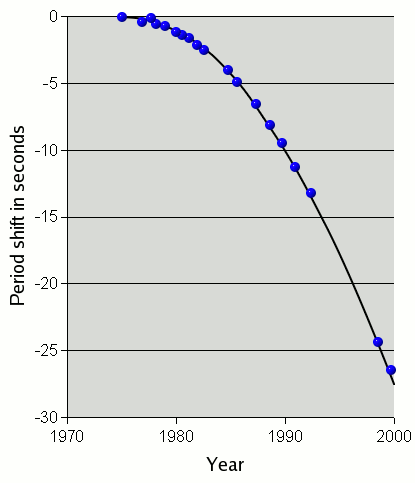
\includegraphics[scale=0.90]{Images/PSR.png}
\caption{The periastron period shift plotted against time, for the Hulse--Taylor PSR1913+16 binary pulsar. The companion arrives earlier at the periastron due to the decrease in separation, hence showing a decrease of the orbital period. Continuous line represents the predicted evolution due to emission of GW and the dots represent the observational data. The system is highly eccentric, and the losses in energy and angular momentum increase significantly as the eccentricity approaches one, i.e., as the ellipse of the orbit becomes more elongated. Image reproduced from \cite{Weisberg:2004hi}}
\label{fig:hulsepulsar}
\end{figure}

Another binary pulsar, PSR J0737--3039, shows the same decrease in orbital period due to \ac{GW} emission. Differently from PSR B1913+16, the components are both seen as pulsars and the orbital plane is almost face--on. This allows the dynamics of this system to be observed to a greater degree of accuracy than is possible with other binary systems and general relativity to be tested in a number of ways. Gravitational redshift and rate of change of the periastron could be accurately measured using data from PSR J0737--3039. All observations have been fully consistent with the predictions of general relativity \cite{Kramer:2006nb, Kim:2006fm}. In \cite{Kramer:2006nb} it is quoted that observations of this system agree with general relativity within an error of only 0.05\%.

An interesting example of indirect \ac{GW} observation is OJ 287, a BL Lacertae object that is believed to be a supermassive binary black hole system (SMBBH). The binary components are of asymmetric masses -- a supermassive black hole with a mass of $\sim 18 \times 10^9 M_{\odot}$ and a companion black hole with a mass of $\sim 10^8 M_{\odot}$. Since this object has been observed for almost 120 years, it was noticed that it displays a periodic variation in its visible magnitude that has a 12 year cycle with two outbursts at 12 year intervals. The supermassive black hole binary model would fit the observations as the system is modelled as the companion orbiting the primary on a moderately elliptical orbit, the emission peaks would occur as the companion's orbit intersects the primary's accretion disk. The times of the outbursts can be explained if the system emitted \ac{GW} \cite{Nature:0804, Sivaram:2008jy}.

\section{Linearized Gravity and Gravitational Waves}
 
Linearized gravity is an approximation in the study of general relativity in which the nonlinear contributions from the spacetime metric are ignored. This approach simplifies the calculations for many problems where approximate results can be used instead of the exact solutions. Linearized gravity is sometimes seen as flat space--time gravity with a small perturbation. One of the most important applications for linearized gravity is gravitational waves.

This section will give a brief overview of the theory behind \ac{GW}. We will focus on the linearized theory of \ac{GW} as described in \cite{MTW, Sch85, Maggiore:gw, 1999physics8041C}. We will closely follow the formalism and workflow given in these references. Therefore, this section will serve as foundation for the other chapters but is not intended as an in--depth description of the \ac{GW} theory, and we point the reader to consult the above mentioned references for a comprehensive analysis.

\subsection{Einstein's field equations and the weak--field approximation}
Einstein's field equations are a set of ten equations that describe quantitatively Einstein's theory of general relativity. They define gravity in terms of the curvature of space--time due to presence of matter and energy. In the standard tensor notation they are given by:
%
\begin{equation}
\label{eq:einsteins}
G_{\mu \nu} = R_{\mu \nu} - \frac{1}{2} g_{\mu\nu}R = \frac{8\pi G}{c^4} T_{\mu \nu} 
\end{equation}
%
where $R_{\mu \nu}$ is the Ricci tensor, $R$ the Ricci scalar and $g_{\mu\nu}$ the metric tensor of four--dimensional space--time. The Riemannian curvature tensor is defined as
\begin{equation}
R^{\mu}_{~\gamma\alpha\nu} = \frac{\partial \Gamma^{\mu}_{~\alpha\gamma}}{\partial x^{\nu}} - \frac{\partial \Gamma^{\mu}_{~\nu\gamma}}{\partial x^{\alpha}} + \Gamma^{\mu}_{~\nu\beta}~\Gamma^{\beta}_{~\alpha\gamma} - \Gamma^{\mu}_{~\alpha\beta}~\Gamma^{\beta}_{~\nu\gamma}
\end{equation} 
%
where $\Gamma$ is the {\it Christoffel symbol} or the {\it affine connection} defined as: 
\begin{equation}
\Gamma^{\mu}_{~~\alpha\beta} = \frac{1}{2} g^{\mu\nu}\left(
\frac{\partial g_{\nu\alpha}}{\partial x^{\beta}} +
\frac{\partial g_{\beta\nu}}{\partial x^{\alpha}} -
\frac{\partial g_{\alpha\beta}}{\partial x^{\nu}}\right)
\end{equation}
%
The Ricci tensor is:
%
\be R_{\mu \nu} = R^{\alpha}_{\mu\alpha\nu} \ee
%
and the Ricci scalar is:
%
\be R = g^{\mu \nu}R_{\mu\nu}, \ee
%
In a ``flat'' space,
%
\begin{equation}
R^{\mu}_{~\gamma\alpha\nu} = 0.
\end{equation}
%
$T_{\mu \nu}$ is the stress energy tensor, which describes the density and flux of matter (or energy) and momentum. The components of this tensor may be interpreted in the following way, according to \cite{Sch85}:
%
\begin{itemize}
 \item $T_{00}$ is the energy (or relativistic mass) density.
 \item $T_{0i} = T_{i0}$ is the energy flux in the $i$--th direction, or the density of $i$--momentum.
 \item $T_{ij}$ is flux of $i$--momentum in the $j$--th direction.
\end{itemize}
%
Einstein's equations describe ten equalities, rather than the 16 apparent. This is
because $R_{\mu\nu}$, $g_{\mu\nu}$ and $T_{\mu\nu}$ are all symmetric.

Gravitational waves may be naively seen as {\it ripples} in the space--time fabric created by a strong gravitational field source. Our analysis follows the weak--field approximation, therefore we place the observer far away from the putative source. We will consider that the gravitational field at the observer is \emph{weak} but not \emph{static}. Also, consider that there are no restrictions on the motion of particles in the vicinity of the observer. In the absence of gravitational interaction, space--time is flat and is characterized by the Minkowski flat metric \cite{1999physics8041C}:
%
\begin{equation}
\eta = \left( \begin{array}{cccc}
           -1 & 0 & 0 & 0 \\
	    0 & 1 & 0 & 0 \\
	    0 & 0 & 1 & 0 \\
            0 & 0 & 0 & 1 \end{array} \right)
\end{equation}
%
A weak gravitational field can be considered as a small ``perturbation'' on the flat Minkowski metric \cite{MTW,Sch85,Maggiore:gw},
%
\begin{equation}
g_{\mu\nu} = \eta_{\mu\nu} + h_{\mu\nu}, ~~~||h_{\mu\nu}|| \ll 1
\end{equation}

\noindent The condition $||h_{\mu\nu}|| \ll 1$ shows that the analysis is done in a weak gravitational field. Here $||h_{\mu\nu}||$ is defined as the magnitude of a typical non--zero component of $h_{\mu\nu}$. In linearized gravity, the smallness of the perturbation means that we only keep terms which are linear in $h_{\mu\nu}$ (approximation to first order), higher order terms are discarded. As a consequence, indices are raised and lowered using the flat metric $\eta_{\mu\nu}$ . The metric perturbation $h_{\mu\nu}$ transforms as a tensor under Lorentz transformations. We can therefore write,

\begin{equation}
g^{\mu\nu} = \eta^{\mu\nu} - h^{\mu\nu}
\end{equation}

Under a background Lorentz transformation \cite{Sch85}, the perturbation 
transforms as a second--rank tensor:

\begin{equation}
h_{\alpha\beta} = \Lambda_{\alpha}^{~~\mu} \Lambda_{\beta}^{~~\nu} ~h_{\mu\nu}
\end{equation}

The equations obeyed by the perturbation, $h_{\mu\nu}$, are obtained by
writing Einstein's equations to first order. To first order, the 
Christoffel symbol is \cite{MTW,Sch85,Maggiore:gw},

\begin{equation}
\Gamma^{\lambda}_{~~\mu\nu} = \frac{1}{2} \eta^{\lambda\rho}[\partial_{\mu}
h_{\rho\nu} + \partial_{\nu}h_{\mu\rho} - \partial_{\rho}h_{\mu\nu}] + 
{\cal{O}}(h^2)
\end{equation} 

Therefore, the Riemann curvature tensor will reduce to

\begin{equation}
R_{\mu\nu\rho\sigma} = \eta_{\mu\lambda}\partial_{\rho}\Gamma^{\lambda}_{~\nu\sigma} - \eta_{\mu\lambda}\partial_{\sigma}\Gamma^{\lambda}_{~\nu\rho}
\end{equation}

The Ricci tensor is obtained to first order in $h$:

\begin{equation}
R_{\mu\nu} \approx R^{(1)}_{\mu\nu} = \frac{1}{2}\left[\partial_{\lambda}\partial_{\nu}h^{\lambda}_{~\mu} + \partial_{\lambda}\partial_{\mu}h^{\lambda}_{~nu} - \partial_{\mu}\partial_{\nu}h - \Box h_{\mu\nu}\right]
\end{equation}
%
where, $\Box = \eta^{\lambda\rho}\partial_{\lambda}\partial_{\rho}$ is 
the D'Alembertian in flat space--time. Contracting with $\eta^{\mu\nu}$,
the Ricci scalar is:

\begin{equation}
R = \partial_{\lambda}\partial_{\mu} h^{\lambda\mu} - \Box h
\end{equation}
%
The Einstein tensor, $G_{\mu\nu}$, in the limit of weak gravitation is given by:

\begin{equation}
G_{\mu\nu} = R_{\mu\nu} - \frac{1}{2} \eta_{\mu\nu} R = \frac{1}{2}[\partial_{\lambda}\partial_{\nu}h^{\lambda}_{\mu} + \partial_{\lambda}\partial_{\mu}h^{\lambda}_{~\nu} - \eta_{\mu\nu}\partial_{\mu}\partial_{\nu}h^{\mu\nu} + \eta_{\mu\nu}\Box h - \Box h_{\mu\nu}]
\label{infnsol}
\end{equation}
%
For simplicity one can choose geometric coordinates $c=G=1$. 

Equation set (\ref{infnsol}) will have an infinite number of solutions. The decomposition of $g_{\mu\nu}$ in the weak gravitational field approximation does not completely specify the coordinate system in space--time. In solving Einstein’s equations it is common practice to impose gauge conditions: one adds new conditions on the metric tensor until the coordinate system is uniquely fixed. After four gauge conditions are imposed (the number of degrees of freedom in choosing the coordinate system), the metric is determined.
When we have a system that is invariant
under a gauge transformation, we {\it fix} the gauge and work in a selected 
coordinate system. One such coordinate system is the Lorentz gauge coordinate system, the gauge in which linearized gravity is simplest \cite{1999physics8041C, Maggiore:gw}. The gauge condition is called {\it Lorentz gauge}:
%
\begin{equation}
g^{\mu\nu}\Gamma^{\lambda}_{~~\mu\nu} = 0 
\end{equation}
%
In the weak field limit, this condition reduces to 
%
\begin{equation}
\partial_{\lambda} h^{\lambda}_{~~\mu} = \frac{1}{2}\partial_{\mu} h
\end{equation}
%
In this chosen gauge, the linearized Einstein equations simplify to:
%
\begin{equation}
\Box h_{\mu\nu} - \frac{1}{2} \eta_{\mu\nu}\Box h = - 16 \pi G T_{\mu\nu}
\end{equation}
%
The trace--reversed perturbation, $\bar{h}_{\mu\nu}$, is defined as follows:
%
\begin{equation}
\bar{h}_{\mu\nu} = h_{\mu\nu} - \frac{1}{2}\eta_{\mu\nu} h
\end{equation}
%
The Lorentz gauge condition further reduces to:
%
\begin{equation}
\partial_{\mu} \bar{h}^{\mu}_{~\lambda} = 0
\end{equation}
%
The Einstein equations are then:
%
\begin{equation}
\Box \bar{h}_{\mu\nu} = - 16 \pi G T_{\mu\nu}
\end{equation}
%
The above equation is written in the presence of matter and energy. If written in vacuum, 
where the stress--energy tensor will vanish, we obtain the familiar plane waves equation:
%
\begin{equation}
\Box \bar{h}_{\mu\nu} = 0
\end{equation}
%
The vacuum equations for $\bar{h}_{\mu\nu}$ are similar to the wave 
equations in electrodynamics or acoustics. 
These second order partial differential equations will have plane--wave solutions of the type:
%
\begin{equation}
\bar{h}_{\mu\nu} = B_{\mu\nu} {\rm e}^{i k_{\alpha}x^{\alpha}}
\label{hsolution}
\end{equation}
%
where, $B_{\mu\nu}$ is a constant, symmetric second rank tensor and $k_{\alpha}$
is a constant four--vector known as the {\it plane wave vector} satisfying 
%
\begin{equation}
k_{\alpha}k^{\alpha} = 0
\end{equation}
%
This shows that a solution (\ref{hsolution}) is possible
if $k_{\alpha}$ is {\it null} -- tangent to the world line of a
photon, i.e., gravitational waves propagate at the speed of light $c$ in vacuum. Since we used the $c=G=1$ notation convention, it is not straightforward to see that, in fact,  $c$ is a conversion factor used in order to change the units of time to units of space. This makes it the only speed which does not depend either on the motion of an observer or of a gravitational waves source, therefore $c$ is also the speed of gravitational waves and any other massless particle (like the photon). The time--like component of the wave vector is referred to as the 
{\it frequency} of the wave. The four--vector, 
$k_{\alpha}$ is usually written as $k_{\alpha} \equiv (\omega, {\bf k})$.
%
\begin{equation}
\omega_{gw}^2 = |{\bf k}|^2
\end{equation}
%
This represents the {\it dispersion relation} for the 
gravitational waves. The plane wave is completely described by a number of 
independent parameters: ten from the coefficients $B_{\mu\nu}$ and three 
from the null vector $k_{\alpha}k^{\alpha} = 0$.

\subsection{Transverse traceless gauge}
We use the Lorentz gauge to prove that that gravitational radiation
will propagate in vacuum as transverse plane waves at the speed of light $c$. There
are, however, further gauge freedoms that can be used to further simplify the form
of $h_{\mu\nu}$ . Using the Lorentz gauge condition, one obtains as follows:
%
\begin{equation}
k_{\alpha} B^{\alpha\beta} = 0 
\end{equation}
%
This imposes a restriction on $B^{\alpha\beta}$ : it is orthogonal 
({\it transverse}) to $k_{\alpha}$. The number of independent 
components of $B_{\alpha\beta}$ is thus reduced to six.
It can be easily proved that any coordinate transformation of the form
%
\begin{equation}
x^{\alpha^{\prime}} = x^{\alpha} + \xi^{\alpha}(x^{\beta})
\end{equation}
%
will leave the plane wave equation
%
\begin{equation}
\Box x^{\mu} = 0
\end{equation}
%
satisfied as long as
%
\begin{equation}
\Box \xi^{\alpha} = 0
\end{equation}
%
One can therefore choose a solution
%
\begin{equation}
\xi_{\alpha} = C_{\alpha} {\rm e}^{i k_{\beta} x^{\beta}}
\end{equation}
%
to the wave equation for any $\xi_{\alpha}$. $C_{\alpha}$ are constant 
coefficients. If
%
\begin{equation}
B^{\mu}_{\mu} = 0 ~~~~({\rm \it traceless})
\end{equation}
%
and
%
\begin{equation}
B_{\mu\nu} V^{\beta} = 0
\end{equation}
%
where, $V^{\beta}$ is some fixed four--velocity, that is, any constant 
time dependent unit vector one wishes to choose. The equations
%
\begin{equation}
k_{\alpha} B^{\alpha\beta} = 0 \hspace{1cm}
B^{\mu}_{\mu} = 0 \hspace{1cm}
B_{\mu\nu} V^{\beta} = 0
\end{equation}
%
are called the the {\it transverse--traceless} (TT) gauge 
conditions \cite{Sch85}. The trace condition $B^{\mu}_{\mu} = 0$ implies that
%
\begin{equation}
\bar{h}^{TT}_{\alpha\beta} = h^{TT}_{\alpha\beta}
\end{equation}


Consider now a background Lorentz transformation in
which the vector $V^{\alpha}$ is the time basis vector $V^{\alpha} = 
\delta^{\alpha}_{~0}$. Then the third TT equation implies that $B_{\mu 0} = 0$ for all
$\mu$. Further consider a privileged orientation of the coordinate axes so that the wave is travelling 
along the $z$-direction, $k^{\mu} \rightarrow (\omega_{gw}, 0, 0, \omega_{gw})$. 
Then with the TT equations it implies that $B_{\alpha z} = 0$ for all
$\alpha$. The $xx$ and $xy$ components of the amplitude tensor are also called the polarizations and labelled as $xx \equiv +$ and $xy \equiv \times$ as in the following ~\cite{Maggiore:gw, 1999physics8041C}:

\begin{equation}
B^{TT}_{\alpha\beta} = \left( \begin{array}{cccc}
              0 & 0 & 0 & 0 \\
              0 & B_+ & B_{\times} & 0 \\
              0 & B_{\times} & -B_{+} & 0 \\
              0 & 0 & 0 & 0 \end{array} \right)
\label{eqn:polarizations}
\end{equation}
 
To obtain the solution of the linearized wave equations, the Green's function method will be used \cite{Sch85, 1999physics8041C}.
The Green's function, $G(r_1^{\mu} - r_2^{\mu})$, of the D'Alembertian 
operator $\Box$, is the solution of the wave equation in the presence of 
a delta function source:
%
\begin{equation}
\Box~G(r_1^{\mu} - r_2^{\mu}) = \delta^{(4)}(r_1^{\mu} - r_2^{\nu})
\end{equation}
%
where $\delta^{(4)}$ is the four--dimensional Dirac delta function of spatial coordinates and time. The 
general solution to the linearized Einstein's equations can be 
written using Green's function as
%
\begin{equation}
\bar{h}_{\mu\nu}(r_1^{\alpha}) = - 16\pi G\int \mathrm{d}^4 r_2~G(r_1^{\alpha} - r_2^{\alpha})
T_{\mu\nu}(r_2^{\alpha})
\end{equation}
%
The solutions to this equation are called {\it advanced} or {\it retarded}
according as they represent waves travelling backward or 
forward in time, respectively. We are interested in the retarded Green's 
function as it represents the net effect of signals from the past of the point
under consideration. It is given by
%
\begin{equation}
G(r_1^{\mu} - r_2^{\mu}) = - \frac{1}{4\pi |{\bf r_1} - {\bf r_2}|}
\delta\left[ |{\bf r_1} - {\bf r_2}| - (r_1^0 - r_2^0)\right]\times~\theta(r_1^0 - r_2^0)
\end{equation}
%
where, ${\bf r_1} = (r_1^1, r_1^2, r_1^3)$ and ${\bf r_2} = (r_2^1, r_2^2, r_2^3)$ and
$|{\bf r_1} - {\bf r_2}| = [\delta_{ij}(r_1^{i} - r_2^{i})(r_1^{j} - r_2^{j})]^{1/2}$.
$\theta(r_1^{0} - r_2^{0})$ is the Heaviside unit step function, it equals
1 when $r_1^0 > r_2^0$, and equals 0 otherwise. We can perform the integral over the time--like component $r_2^0$ with the help of the delta 
function, switching to a space--like integral (denoted by arguments in bold)
%
\begin{equation}
\bar{h}_{\mu\nu}(t, {\bf r_1}) = 4G\int \mathrm{d}^3 {\bf r}_2~\frac{1}{|{\bf r}_1 - {\bf r}_2|}
T_{\mu\nu}(t - |{\bf r}_1 - {\bf r}_2|, {\bf r}_2) 
\end{equation}
%
The quantity
%
\begin{equation}
t_{\rm r} = t - |{\bf r}_1 - {\bf r}_2|
\end{equation}
%
is called the {\it retarded time} with ${\bf D}= {\bf r}_1- {\bf r}_2$. From the expression for $\bar{h}_
{\mu\nu}$, it is easy to observe that the perturbation in the gravitational field at 
$(t, {\bf r}_1)$ is a sum of the influences from the energy and momentum 
sources at the points $(t_{\rm r}, {\bf r}_2)$ in the past light cone.

\subsection{Mass quadrupole}
One can now consider the gravitational radiation
emitted by an isolated far away source consisting of very slowly moving 
particles (the spatial dimensions of the source are neglected compared 
to the distance between the source and the observer) \cite{1999physics8041C, Maggiore:gw}. The Fourier 
transform of the perturbation $h_{\mu\nu}$ is 
%
\begin{equation}
{\tilde{h}}_{\mu\nu} (\omega_{gw}, {\bf r}_1) = \frac{1}{\sqrt{2\pi}}\int {\rm d}t~{\rm e}^
{i\omega_{gw} t}~h_{\mu\nu}(t, {\bf r}_1)
\end{equation}
%
Using the expression for $h_{\mu\nu} (t, {\bf r}_1)$, one obtains
%
\begin{equation}
{\tilde{h}}_{\mu\nu} = 4\int {\rm d}^3 {\bf r}_2 ~{\rm e}^{i\omega_{gw} |{\bf r}_1 - 
{\bf r}_2|}~\frac{\tilde{T}_{\mu\nu}(\omega_{gw}, {\bf r}_2)}{|{\bf r}_1 - {\bf r}_2|}
\end{equation}
%
Under the assumption that the spatial extent of the source is much smaller
compared to the distance between the source and the observer, one can replace
the term ${\rm e}^{i\omega_{gw} |{\bf r}_1 - {\bf r}_2|}/|{\bf r}_1 - {\bf r}_2|$ 
in by ${\rm e}^{i\omega_{gw}{\rm D}}/{\rm D}$. Therefore,
%
\begin{equation}
\tilde{h}_{\mu\nu}(\omega_{gw}, {\bf r}_1) = 4~\frac{{\rm e}^{i\omega_{gw}
{\rm D}}}{{\rm D}}~\int {\rm d}^3 {\bf r}_2~\tilde{T}_{\mu\nu}(\omega_{gw}, {\bf r}_2)
\end{equation}
%
The Lorentz gauge condition in Fourier space is 
%
\begin{equation}
\partial_{\mu}h^{~\mu\nu}(t, {\bf r}_1) = \partial_{\mu}\int {\rm d}\omega_{gw}~
{\tilde{h}}^{~\mu\nu}~{\rm e}^{-i\omega_{gw} t} = 0
\end{equation}
%
We introduce the Fourier spatial version of the conservation of energy equation for 
$T^{\mu\nu}$: 
%
\begin{equation}
\partial_{\mu} T^{\mu\nu}(t, {\bf r}_1) = 0
\end{equation}
%
and the {\it quadrupole moment tensor} of the energy--density of the source \cite{Sch85}:
%
\begin{equation}
\tilde{M}_{ij}(\omega_{gw}) = \int {\rm d}^3 {\bf r}_2~r^{i}r^{j}~\tilde{T}^{00}(\omega_{gw}, {\bf r}_2)
\end{equation}
%
With respect to the newly defined quadrupole moment tensor, we have
%
\begin{equation}
\int {\rm d}^3 {\bf r}_2~\tilde{T}^{ij}(\omega_{gw}, {\bf r}_2) = - \frac{\omega_{gw}^2}{2}~
\tilde{M}_{ij}(\omega_{gw})
\end{equation}
%
Hence, the solution reads
%
\begin{equation}
\tilde{h}_{ij}(\omega_{gw}, {\bf r}_1) = -2~\frac{\omega_{gw}^2}{{\rm D}}
~{\rm e}^{i\omega_{gw}{\rm D}}~\tilde{M}_{ij}(\omega_{gw})
\end{equation}
%
The final expression of the metric perturbation is obtained after a last Fourier transform:
%
\begin{equation}
h_{ij}(t, {\bf r}_1) = \frac{2}{{\rm D}}~\frac{{\rm d}^2}{{\rm d}t^2}~M_{ij}(t_{{\rm r}})
\end{equation}
%
where, $t_{{\rm r}} = t - |{\bf r}_1 - {\bf r}_2|=t - D$ is the retarded time. To re--write this expression in SI units, we have:
%
\begin{equation}
h_{ij}(t, {\bf r}_1) = \frac{2G}{c^4{\rm D}}~\frac{{\rm d}^2}{{\rm d}t^2}~M_{ij} \left (t - \frac {|{\bf r}_1 - {\bf r}_2|}{c} \right )
\label{inertia}
\end{equation}
%
Up to now we have assumed that $\ddot{M}_{ij}$ is evaluated in the transverse--traceless frame, with the gravitational radiation propagating along the $z$ direction. This is commonly called the ``radiation frame''. ``Radiation frame'' differs from the ``source frame'', or the frame associated with the source itself: the source (e.g., a compact binary system) lies in an $x'-y'$ plane that is different from the radiation $x-y$ plane. To obtain the new expression for $h_{ij}(t, {\bf r}_1)$ in the ``source frame'' we need to apply a rotation ${\rm \bf R}={\rm \bf R}(\iota, \varphi)$ matrix with the angles $(\iota, \varphi)$ shown in Figure \ref{fig:intro_det_source}. We will need three angles in order to rotate the ``source frame'' into
the ``radiation frame'' that will reduce to two angles if we consider the radiation is travelling in the $z$ direction. Explicitly, the radiation frame is related to the source frame 
%
\begin{figure}[tp]
  \centering
  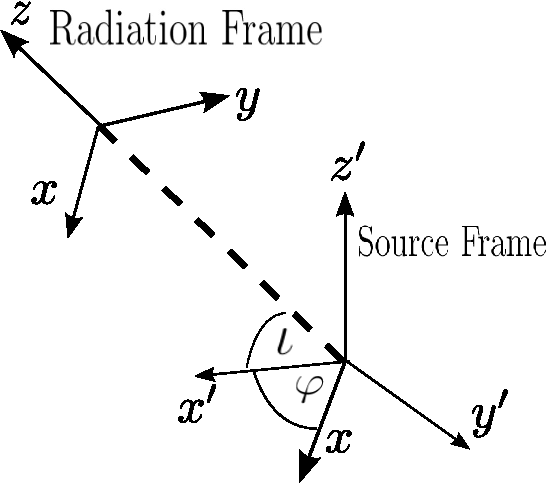
\includegraphics[width=0.5\linewidth]{Images/skyangles2.pdf}
  \caption[The angles that describe the relationship between the source
and radiation frames.]{\label{fig:intro_det_source}
A diagram that shows the geometric conversion from a ``radiation frame'' ($x-y$) to a ``source frame'' ($x'-y'$). Figure originally published in \cite{Mckechan:2010}.}
\end{figure}
%
\bea \left( \begin{array}{c} x' \\ y' \\ z' \end{array} \right)=
\left( \begin{array}{ccc}
\cos \varphi & - \sin \varphi & 0 \\
\sin \varphi & \cos \varphi & 0 \\
0 & 0 & 1
\end{array} \right)
\left( \begin{array}{ccc}
1 & 0 & 0 \\
0 & \cos \iota & -\sin \iota \\
0 & \sin \iota & \cos \iota
\end{array} \right)
\left( \begin{array}{c} x \\ y \\ z \end{array} \right)
\eea
%
\be \left( \begin{array}{c} x' \\ y' \\ z' \end{array} \right)=
R
\left( \begin{array}{c} x \\ y \\ z \end{array} \right) \ee
%
The new ``source'' quadrupole moment will then be defined as:
%
\begin{equation}
M_{ij}' = {\rm \bf R}^T(\theta, \phi)~M_{ij}~{\rm \bf R}(\theta, \phi)
\end{equation}
%
The equation for $h_{ij}$ is then written as ~\cite{Maggiore:gw, 1999physics8041C}
%
\be \label{eq:intro_h_dom}
h_{ij}^{TT}(t) = \frac{2}{D} \ddot{M}_{ij} \left(t - D\right). \ee
%
and the $h_+$ and $h_{\cross}$ components are given by
%
\be h_{+} = \frac{1}{D} \left(\ddot{M}_{11} - \ddot{M}_{22}\right) \ee
\be h_{\cross} = \frac{2}{D} \ddot{M}_{12}. \ee
%
Rotating the ``source'' quadrupole moment into the ``radiation frame'' we can write the
$h_+$ and $h_{\cross}$ components of the gravitational radiation as function of components of ``source'' moments $\ddot{M}'_{ij}$:
%
\begin{subequations}
\label{eq:gwemissionmain}
 \begin{align}
h_+ = \frac{1}{D} &\biggl[\ddot{M}'_{11}\left(\cos^2\varphi - \sin^2\varphi
\cos^2\iota\right) \nonumber \\ \nonumber &+ \ddot{M}'_{22}
\left(\sin^2\varphi - \cos^2 \varphi \cos^2\iota
\right) \\&- \ddot{M}'_{33}\sin^2 \iota - \ddot{M}'_{12}\sin 2\varphi
\left(1+ \cos^2 \nonumber
\theta\right) \\ &+ \ddot{M}'_{13} \sin\varphi \sin 2\iota + \ddot{M}'_{23}
\cos \varphi
\sin2\iota \biggr]
\label{eq:gwemission006}\\
h_{\cross} = \frac{1}{D} &\biggl[ \left(\ddot{M}'_{11} - \ddot{M}'_{22}\right)
\sin2\varphi \cos\iota + 2\ddot{M}'_{12}\cos2\varphi\cos\iota \nonumber
 \\ &- 2\ddot{M}'_{13}\cos
\varphi\sin\iota + 2\ddot{M}'_{23}\sin\varphi\sin\iota\biggr] .
\label{eq:gwemission007}
\end{align}
\end{subequations}
While higher order multipole moments of the mass distribution can contribute to the radiation, for most systems the quadrupole will dominate. Further, the mass monopole and dipole moment will not contribute any gravitational waves. Thus, such events as a spherically symmetric gravitational collapse and axially symmetric rotation do not emit any gravitational radiation. On the other hand, a rotating dumbbell is an excellent emitter of gravitational waves, making binary systems potentially amongst the brightest emitters of gravitational waves in the Universe.

\section{Gravitational waves from a compact binary coalescence} 
Two compact stars (two neutron stars, two black holes or a neutron star and a black hole) orbit each other in a 
close orbit and due to the very strong gravitational field produced by this system, gravitational waves are emitted. By emitting gravitational waves, the system loses energy and angular momentum hence the separation between the objects lessens with every orbit. The closer the stars get to each other, the more orbital energy is converted into gravitational waves, hence, the stronger the gravitational wave emission is. Eventually, the two compact objects will merge. This is called a compact binary coalescence, or CBC event. This system can be easily modelled analytically, in a Newtonian approximation, as described below. Using this approximation, we will derive the gravitational radiation waveform emitted from a \ac{CBC} event with point--like components (masses). This derivation will closely follow the formalism and workflow previously presented in \cite{Maggiore:gw,ian}, and we invite the reader to consult these references (and references therein) for a more detailed explanation.

\subsection{Compact binary coalescence parameters}

Let us consider now a Keplerian binary system far away from an observer $O$. It will be useful to begin by enumerating the physical parameters that are used in defining a \ac{CBC} system. These definitions will be used throughout all of the next chapters. A non--spin components \ac{CBC} on circular orbits can be completely described by nine physical parameters; these are the following:
%
\begin{itemize}
 \item The two masses, ($m_1$, $m_2$),
 \item The coalescence time of the signal at an observer at Earth, $t_c$,
 \item The sky location of the source -- two angles, ($\theta$,$\phi$),
 \item The distance to the source, $D$,
 \item The inclination angle, $\iota$,
 \item The coalescence phase, $\Psi_c$,
 \item The polarization phase, $\psi$.
\end{itemize}
%
The masses of the system are often combined in a number of different ways, these are
given by
%
\begin{itemize}
 \item The total mass, $M$ = $m_1$ + $m_2$,
 \item The chirp mass, $\mathcal{M} = \frac{(m_1 m_2)^{3/5}}{(m_1 + m_2)^{1/5}}$,
 \item The symmetric mass ratio, $\eta = \frac{m_1 m_2}{(m_1 + m_2)^2}$,
 \item The reduced mass, $\mu = \frac{m_1 m_2}{m_1 + m_2}$.
\end{itemize}
%
We also use the following binary orbit--related definitions;
%
\begin{itemize}
 \item The \textit{orbital} phase of the system, $\Psi$,
 \item The phase \textit{of the dominant mode of the emitted signal}, $\Phi = 2\Psi$,
 \item The \textit{orbital} angular frequency, $\omega$,
 \item The frequency \textit{of the emitted GW signal}, $f_{gw}$,
 \item The orbital radius of the system, $r$.
\end{itemize}

\subsection{Time evolution of the system}

Let's consider now equation (\ref{inertia}) for which we would like to find a solution only for the dominant order terms in $\lvert \mathbf{r}_1 - \mathbf{r}_2\rvert$. We consider such a system of two inspiralling compact objects, orbiting each other around the common center of mass (CM). The orbit is considered plane circular and obeying the classical Keplerian laws for celestial mechanics. The system can be considered in quasi--equilibrium  at any given time $t$ much smaller than the coalescence time if
%
\begin{equation}
\frac {{\rm d} \omega(t)}{{\rm d}t} \ll \omega^2(t)
\end{equation}
%
The separation vector ${\bf r}=(r_i(t))$ between the binary components will decrease gradually and reach zero at merger. In plane, Cartesian coordinates, the system is described by the position coordinates with respect to the center of mass:
%
\begin{equation}
r_1(t) = |{\bf r}| \cos (\omega t+ \phi_0), \hspace{10mm}
r_2(t) = |{\bf r}| \sin (\omega t+ \phi_0), \hspace{10mm}
r_3(t)=0
\end{equation}
%
In the center of mass of the system the moment of inertia (the second mass moment) is:
%
\begin{equation}
M^{ij} = \mu~r^i(t)~r^j(t)
\end{equation}
%
where $\mu=m_1m_2/(m_1+m_2)$ is the reduced mass.
If we differentiate this with respect to time twice we obtain
%
\begin{eqnarray}
\label{eq:mdoudbledot}
\ddot{M}_{11} &=& -\ddot{M}_{22} = 2\mu r^2\omega^2 \cos\left(2\int_0^{t}\omega(t') dt'\right) \\
\ddot{M}_{12} &=& - 2\mu r^2\omega^2 \sin\left(2\int_0^{t}\omega(t') dt'\right) \\
\ddot{M}_{13} &=& \ddot{M}_{23} = \ddot{M}_{33} = 0,
\end{eqnarray} 
%
where we assume that $r \omega \gg \dot{r}$. When this is not true the system is
not in a true circular motion.

We will write the solution to equation (\ref{inertia}) given by equations (\ref{eq:gwemission006}) and (\ref{eq:gwemission007}) in a geocentric reference frame:

\begin{subequations}
\begin{align}
h_{+} &= \frac{2\mu\omega^2 r^2}{D} \left( 1 + \cos^2 \iota \right)
\cos\left(\Phi(t) + 2\varphi\right) \\
h_{\cross} &= -\frac{2\mu \omega^2 r^2}{D} 2\cos \iota \sin
\left(\Phi(t)+ 2\varphi\right),
\end{align}
\end{subequations}
%
where the gravitational wave phase is defined as
%
\be \label{eq:cbc_grav_phase} \Phi(t) = 2\int_0^{t}\omega(t') dt'. \ee
%
Expanding $r$ in terms of $\omega$ by using Kepler's third law of planetary motion:
%
\be \omega^2 = \frac{m_1 + m_2}{r^3}. \ee
%
we can then write $h_+$ and $h_{\cross}$ as
%
\begin{subequations}
\label{eq:cbc_hplus_cross}
\begin{align}
h_{+}(t) &= \frac{2}{D}\mathcal{M}^{5/3}\omega(t)^{2/3}\left( 1 + \cos^2 \iota \right)
\cos\left(\Phi(t)+ 2\varphi\right) \\
h_{\cross}(t) &= -\frac{2}{D}\mathcal{M}^{5/3}\omega(t)^{2/3} (2\cos \iota) \sin \left(
\Phi(t)+ 2\varphi\right).
\end{align}
\end{subequations}

\subsection{Energy loss in the system}
\label{sec:cbc_energyloss}

Due to emission of \ac{GW}, the orbital angular velocity $\omega$ will increase with time. Expressing $\omega = \omega(t)$, we can find a measure of the rate at which the system radiates \ac{GW} energy. The total radiated energy in time can be obtained by integrating the time--dependent flux, then the power radiated by a gravitational wave is given as \cite{Maggiore:gw,ian}
%
\be \frac{\mathrm{d}E}{\mathrm{d}t} = \frac{1}{16 \pi} \int d\Omega \langle \dot{h}_+^2 +
\dot{h}_{\cross}^2 \rangle. \ee
%
Equation (\ref{eq:intro_rad_power}) gives us a general formula for the energy loss, to leading order:
%
\be
\label{eq:intro_rad_power}
\frac{\mathrm{d}E}{\mathrm{d}t} = \frac{1}{5} \langle \dddot{M}'_{ij} \dddot{M}'^{ij}
- \frac{1}{3}(\delta^{kl}\dddot{M}'_{kl})^2\rangle. \ee
%
To obtain the third differential of the moment of inertia, we will perform a further differentiation on equation (\ref{eq:mdoudbledot}):
%
\begin{subequations}
\label{eq:mtripledot}
\begin{align}
\dddot{M}_{11} &= -\dddot{M}_{22} = -4\mu r^2\omega^3 \sin\left(2\int_0^{t}\omega(t') dt'\right) \\
\dddot{M}_{12} &= - 4\mu r^2\omega^3 \cos\left(2\int_0^{t}\omega(t') dt'\right) \\
\dddot{M}_{13} &= \dddot{M}_{23} = \dddot{M}_{33} = 0.
\end{align}
\end{subequations}
%
The power radiated by the system is then calculated by inserting equation (\ref{eq:mtripledot}) into (\ref{eq:intro_rad_power}). Using the assumption that for circular orbits $\langle \sin^2 \Phi(t) \rangle = \langle \cos^2 \Phi(t) \rangle = \frac{1}{2}$ we get
%
\be \label{eq:cbcwav_power} P = - \frac{\mathrm{d} E_{orbit}}{\mathrm{d}t} = \frac{32}{5}\left(\mathcal{M} \omega
\right)^{10/3}, \ee
%
which is the total radiated power of the system, to dominant order. The emitted power is proportional to the chirp mass to an exponent $\approx 3$: the heavier the system, the more radiated power. Also, emitted power is proportional to the orbital frequency to an exponent $\approx 3$: the closer the binary components, the higher the frequency thus the more radiated power.

\subsection{Phase evolution of the system}
\label{sec:cbc_phaseevol}

It follows from equation (\ref{eq:cbcwav_power}) that if we write the expression for the total energy of the system, we can compute the time--variance of the orbital angular velocity. Consider the total energy of the system as the sum of kinetic and gravitational potential contributions:
%
\begin{align} \label{eq:cbcwav_etot}
E_{orbit} &= -\frac{m_1 m_2}{r} + \frac{m_1 m_2}{2r} = -\frac{m_1 m_2}{2r} \nonumber \\
&= - \left( \mathcal{M}^5 \omega^2/8\right)^{1/3},
\end{align}
%
differentiate this with respect to time and insert it into equation (\ref{eq:cbcwav_power}) to get
%
\be \frac{32}{5}
\left(\mathcal{M} \omega\right)^{10/3}
=  \mathcal{M}^{5/3} \frac{1}{3}
 \omega^{-1/3} \dot{\omega}. \ee
%
This formula can be rearranged to give the change in orbital angular velocity with
respect to time, $\dot{\omega}$, as
%
\be \dot{\omega} = \frac{96}{5} \mathcal{M}
^{5/3} \omega^{11/3}. \ee
%
The orbital angular frequency can then be expressed as a function of time,
by integrating this equation, provided initial conditions, from a limit time $t_0$ with an initial orbital
frequency $\omega_0$
%
\be \omega(t) = \left(-\frac{256}{5} \mathcal{M}
^{5/3}\left( t - t_0 \right) + \omega_0^{-8/3} \right)^{-3/8}. \ee
%
We can see that  for a time $t \rightarrow t_0$ $\omega$ will diverge to infinity. At this limit, the two bodies will not be in circular motion anymore and will start plunging towards each other. But this time is finite and  for simplification let us take this as our limit time, which we will call $t_{c}$, time of coalescence. This choice serves to set $\omega_0^{-8/3}$ to zero. If we introduce a time variable change to
%
\be \tau \equiv t - t_{c} \ee
%
$\omega$ can be re--expressed in terms of $\tau$ as
%
\be \label{eq:omegatau}
\omega(\tau) = \frac{1}{8}\left(\frac{\tau}{5}\right)^{-3/8}
\mathcal{M}^{-5/8},  \ee
%
and in SI units:
%
\be \label{eq:omegatauSI}
\omega(\tau) = \frac{1}{4}\left(\frac{\tau}{5}\right)^{-3/8}
\left({\frac{G\mathcal{M}}{c^3}}\right)^{-5/8},  \ee
%

Now $\Phi(t)$ can be evaluated by combining equations (\ref{eq:cbc_grav_phase}) and (\ref{eq:omegatau})
%
\begin{subequations}
\begin{align}
\Phi(\tau) &= 2\int_{t_{c}}^{\tau}\frac{1}{8}\left(\frac{\tau'}{5}\right)^{-3/8}
\mathcal{M}^{-5/8} d\tau' \\
\label{eq:cbc_phase_tau}
\Phi(\tau) &= 2 \left(\frac{\tau}{5 \mathcal{M}}\right)^{5/8}
 - 2 \left(\frac{t_{c}}{5 \mathcal{M}}\right)^{5/8}.
\end{align}
\end{subequations}
%
Finally, this allows $h_+$ and $h_{\cross}$ to be evaluated in the time domain by combining equations
(\ref{eq:cbc_hplus_cross}), (\ref{eq:omegatau}) and (\ref{eq:cbc_phase_tau}).

\subsection{Frequency domain waveforms}
\label{sec:cbc_freqdom}

It is often useful in gravitational wave searches to express $h_+$ and $h_{\cross}$ in the frequency
domain. This can be done by performing a Fourier transform on $h_+$ and $h_{\cross}$.

Firstly, to express $\tau$ as a function of frequency, equation (\ref{eq:omegatau}) is rearranged, remembering that $\omega = \pi f$, to get
%
\be \label{eq:taufreq}
\tau(f) = \frac{5}{256}(\pi f)^{-8/3} \mathcal{M}^{-5/3}.
\ee
%
Inserting this into equation (\ref{eq:cbc_phase_tau}) gives
%
\be \Phi(f) = \frac{1}{16} f^{-5/3} \mathcal{M}^{-5/3} - 2 \left(\frac{t_{c}}{5 \mathcal{M}}\right)^{5/8}
\label{phasefivethirds}
\ee
%
and the time domain waveforms can be written in terms of the frequency
%
\begin{subequations}
\label{eq:cbc_hp_hc_freq}
\begin{align}
h_{+}(\tau) &= \frac{2}{D} \mathcal{M}^{5/3}
\left( \pi f(\tau) \right)^{2/3}
\left( 1 + \cos^2 \iota \right)
\cos \left(
\Phi(f(\tau)) + 2\varphi\right) \\
h_{\cross}(\tau) &= -\frac{2}{D} \mathcal{M}^{5/3}
\left( \pi f(\tau) \right)^{2/3}
(2\cos \iota)  \sin \left(
\Phi(f(\tau)) + 2\varphi\right).
\end{align}
\end{subequations}
%
To convert this into the Fourier domain, $\tilde{h}_+$ and $\tilde{h}_{\cross}$,
a Fourier transform could be performed on the time domain waveforms. Performing a Fourier transform numerically may often prove to be computationally expensive, hence it is desirable to have an analytical formula for the frequency domain waveforms. This can be obtained by using the \emph{stationary phase approximation} (SPA). This approximation is used in cases of rapidly--varying phase terms. Using \cite{Bro04}, we will define the stationary phase approximation: given a harmonic function with a time--varying amplitude, e.g.,
%
\be F(t) = A(t) \cos(\phi(t)), \ee
%
where
%
\be \frac{1}{A} \frac{\mathrm{d} A}{\mathrm{d}t} \ll \frac{\mathrm{d} \phi}{\mathrm{d}t} \ee
%
at all times $t$; for a GW emitted by a CBC, the phase change over time is much larger than the relative amplitude change over time. The Fourier transform of $F(t)$ can be approximated as
%
\be \tilde{F}(f) \approx \frac{1}{2} A(f) \left(\frac{\mathrm{d}f}{\mathrm{d}t}\right)^{1/2}
\exp\left[ -i \left(2 \pi f t' - \phi(f) - \frac{\pi}{4}\right)\right],
\ee
%
where $t'$ is defined as the time at which
%
\be \left( \frac{\mathrm{d} \phi(t)}{\mathrm{d}t} \right)_{t=t'}= \pi f \ee
%
The stationary phase approximation can be applied to $h_+$ and $h_{\cross}$ to give analytical formulae for the frequency domain waveforms. To evaluate these frequency domain waveforms we first need to evaluate $\frac{\mathrm{d}f}{\mathrm{d}t}$. Using equation (\ref{eq:omegatau}) and $\omega = \pi f$ we get
%
\be \frac{\mathrm{d}f}{\mathrm{d}t} = -\frac{\mathrm{d}f}{\mathrm{d}\tau} = \frac{3}{320 \pi} \left(\frac{\tau}{5}\right)^{-11/8}
\mathcal{M}^{-5/8}, \ee
%
this can be expressed in terms of frequency by substituting equation (\ref{eq:taufreq})
%
\be \frac{\mathrm{d}f}{\mathrm{d}t} = \frac{96}{5} \pi^{8/3} f^{11/3} \mathcal{M}^{5/3}. \ee
%
The stationary phase frequency domain waveforms can then be written, to the leading order, as
%
\begin{subequations}
\label{eq:cbc_hp_hc_spa}
\begin{align}
\tilde{h}_{+}(f) &= \frac{1}{D} \left(\frac{5}{96}\right)^{1/2}
\mathcal{M}^{5/6} \pi^{-2/3} f^{-7/6}
\left( 1 + \cos^2 \iota \right)
\exp \left[ i \left(2\pi f t' -
\Phi(f) - \frac{\pi}{4} - 2\varphi\right)\right] \\
\tilde{h}_{\cross}(f) &= -\frac{1}{D} \left(\frac{5}{96}\right)^{1/2}
\mathcal{M}^{5/6} \pi^{-2/3} f^{-7/6}
(2\cos \iota)
\exp \left[ i \left(2\pi f t' -
\Phi(f) + \frac{\pi}{4} - 2\varphi\right)\right].
\end{align}
\end{subequations}
%
Equations (\ref{eq:cbc_hplus_cross}), (\ref{eq:omegatau}), (\ref{eq:cbc_phase_tau}) and (\ref{eq:cbc_hp_hc_spa}) describe the evolution of the \ac{GW} waveforms from a \ac{CBC} event to first order in both time and frequency domains.

This set of calculations have been derived using a Newtonian mechanics approximation, i.e. considering circular orbits. Introducing relativistic corrections is beyond the scope of this thesis. The Post--Newtonian formalism allows the phase evolution of the binary system to be predicted with much higher accuracy than the approximate derivation given here \cite{Buonanno:2009zt,Bliving}. The Post--Newtonian expansion uses perturbative techniques to expand the phase of the system to higher order terms. Generally the expansion is performed around $(\pi M f)^{1/3}$.

In equation (\ref{phasefivethirds}) we have shown that the leading order term in time domain phase evolution is a multiple of $f^{-5/3}$. The next term, the ``1 PN'' term enters at $f^{-3/3}$, the ``1.5 PN'' term enters
at $f^{-2/3}$ and so on (there is no 0.5 PN term proportional to $f^{-4/3}$). Current non--spinning Post--Newtonian expansions generally include all terms up to 3.5 PN order \cite{Buonanno:2009zt}.

In addition to higher--order phase terms, there are also higher--order amplitude terms. These higher--order amplitude terms arise from the octopole (and consequently higher) moments and therefore the phase of these terms is not necessarily twice the orbital phase. A study of these higher order amplitude terms and how they might affect our ability to detect \ac{CBC} systems can be found in \cite{Mckechan:2010}, but the importance of these higher order amplitude terms is much less than the higher order frequency terms.

Another remark we have to make is that, in general relativistic geometry, there is a minimal radius beyond which circular orbits are no longer possible -- the Innermost Stable Circular Orbit (ISCO). This is defined in Schwarzschild geometry for a point mass around a black hole

\be r_{\mathrm{ISCO}} \equiv \frac{6GM}{c^2} \ee

We may extend this definition to a binary system of compact stars -- this will, of course, be an approximation from the rigorous definition of ISCO. In such a system, the ISCO radius defines the limit between weak--field and strong--field, and using this, the maximum frequency at which the binary is still in a quasi--Keplerian motion is
%
\be f_{\mathrm{ISCO}} = \frac{c^3}{6 \sqrt{6} \pi GM} \ee
%
With this in mind we see that the inspiral phase of a system of binary neutron stars (NS--NS) each with a mass of $m_1 = m_2 \approx 1.4 M_{\odot}$ will end at a frequency of $f \sim 1600$~Hz. For a stellar mass binary black hole system this frequency will reduce to  $f \sim 100-200$~Hz and for a supermassive binary black hole system it will be in the mHz range. These values are very important when building GW detectors: depending on the detectors' construction and subsequent operational frequency window, different GW detectors are sensitive to different GW sources.


\section{Gravitational Wave Detectors -- Theoretical Aspects}

\subsection{A simplified laser interferometer}

The most widely used and altogether the largest and most sensitive type of \ac{GW} detector uses laser light interferometry as functional principle. A simplified schematic of a Michelson laser interferometry GW detector is pictured in Figure ~\ref{ligo_optics}.

\begin{figure}[ht]
\centering
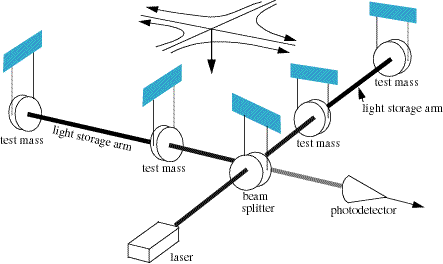
\includegraphics[scale=0.70]{Images/interferometer.png}
\caption{Optical set--up schematics for a \ac{GW} interferometer. Image initially published and adapted from \cite{Abadie:2010px}}
\label{ligo_optics}
\end{figure}

It consists of two arms oriented at a $90^\circ$ angle with laser beams running along the length of the arms. The laser light is emitted at the center of the ``L'' shape and split using a beam splitter, the light then travels along each of the arms, is reflected by mirrors at the end of each arm, passes back down along the arms and is recombined
at the initial starting point. A plane gravitational wave incident to the plane of the detector affects the two ``L'' arms differently, by simultaneously lengthening one while shortening the other. By measuring this differential effect one can measure the \ac{GW} strain. As the path length for the light to travel down the arms varies, the laser light being recombined will have a variable phase difference and thus by observing the interference pattern we can measure the change in path length between the two arms, created by the \ac{GW} passage.  We will briefly describe what are the physical principles based on which such an interferometer will operate. These are described in detail in \cite{Saulson:1994} and we will summarize the main concepts. The electric field of the input laser light is given by
%
\begin{equation} 
|{\bf E}_{\rm in}| = |{\bf E}_0| \mathrm{e}^{2 \pi ift - i \mathbf{k} \cdot \mathbf{x}}
\end{equation}
%
where $f$ is the frequency of the light and $\mathbf{k}$ is the wave vector. $E_0$
denotes the amplitude of the laser light. Consider the beam splitter to be at $\mathbf{x} = 0$.
The beam splitter will send equal power along each arm so that we can describe the light,
transmitted by the beam splitter and travelling down the $x, y$ arms by the electric fields $|{\bf E}_{\rm in}| = (E_{x},~E_{y})$:
%
\begin{equation} 
E_{x} = \frac{E_0}{\sqrt{2}} \mathrm{e}^{2 \pi ift - i \lvert \mathbf{k} \rvert x}
\end{equation}
%
\begin{equation} 
E_{y} = i \frac{E_0}{\sqrt{2}} \mathrm{e}^{2 \pi ift - i \lvert \mathbf{k} \rvert y}
\end{equation}
%
where $T = 1/\sqrt{2}$ is the transmission coefficient and $R = i/\sqrt{2}$ the reflection coefficient.

After the light is reflected at the end of each arm, the electric fields will be given by:
%
\begin{eqnarray}
 E_{x} = \frac{E_0}{\sqrt{2}} \mathrm{e}^{2 \pi if t - i 2 k L_x} \\
 E_{y} = i \frac{E_0}{\sqrt{2}} \mathrm{e}^{2 \pi if t - i 2 k L_y},
\end{eqnarray}
%
where $L_x$ and $L_y$ denote the path length along the $x$ and $y$ arms respectively. After consecutive reflexions and transmissions the light beams are combined at the photodetector and its electric field is expressed as:
%
\be
  E_{\rm out} = i \frac{E_0}{2} \left( \mathrm{e}^{2 \pi if t - 2 ik L_x} + \mathrm{e}^{2 \pi if t - 2 i k L_y}\right).
\ee
%
and can be re--written as:
%
\be
  E_{\rm out} = i E_0 \mathrm{e}^{2 \pi ift - k (L_x + L_y)}
\cos\left(k (L_x - L_y)\right).
\ee
%
The interferometer is locked to the dark fringe, i.e. in the case of equal path lengths $L_x = L_y = L$ the resultant power at the detecting port should be zero. Since the power of a beam of light is proportional to the squared electric field amplitude, we can see that in case of a variation in path length the dark port will have residual power of the order
%
\be
  \Delta P_{\rm out} \propto 1 + \cos\left(2 k (L_x - L_y)\right).
\ee
%
Thus any variation of the relative path length $\Delta L = L_x - L_y$ of the arms would cause a variation in the
power incident on the photodetector.

In this section we have only given a very simplistic description of
how an interferometer works. For a
more comprehensive description of the operation of modern interferometers and
the methods used to increase sensitivity see \cite{Saulson:1994,Maggiore:gw}.

\subsection{Response of an interferometer to a gravitational wave}
\label{section:interferometerresponse}

\subsubsection{The effect of a \ac{GW} at the detector}
In order to illustrate the effect a \ac{GW} would have on the local geometry of a detector we will first use the example of test particles on a ring. Consider a circular string of test masses subject to the passage of a plane monochromatic gravitational wave $h(t)=(h_+, h_{\cross})= (A_+\cos\left(\omega t - \omega z + \phi_0 \right), A_{\cross}\cos\left(\omega t - \omega z + \phi_0 \right))$ -- the wave is fully described by the two polarizations $+,\cross$. We can write the proper distance between any two given points as the interval $ds$:
%
\begin{equation}
ds^2 = g_{\mu\nu}dx^{\mu}dx^{\nu} = (\eta_{\mu\nu} + h_{\mu\nu})dx^{\mu}dx^{\nu}
\end{equation}
%
and expressing the \ac{GW} in terms of the two polarizations
%
\begin{align}
ds^2 = &-c^2dt^2 + dz^2 + \left( 1 + A_+\cos\left(\omega t - \omega z + \phi_0 \right)\right)
dx^2 \\
&+ \left( 1 - A_+\cos\left(\omega t - \omega z + \phi_0 \right)\right)dy^2 +
2A_{\cross}\cos\left(\omega t - \omega z + \phi_0 \right)dxdy.  \nonumber
\label{hONdetector}
\end{align}
%
If we then consider two particles at positions $(x_1,y_1,0)$ and $(x_2,y_2,0)$ the proper distance between them at some arbitrary time $t$ would be given by
%
\begin{align}
ds^2 =& \left( 1 + A_+\cos\left(\omega t - \omega z \right)
\right)\left(x_1-x_2\right)^2 \nonumber
+ \left( 1 - A_+\cos\left(\omega t - \omega z \right)\right)\left(y_1-y_2\right)^2
\\ &+ 2A_{\cross}\cos\left(\omega t - \omega z \right)
\left(x_1-x_2\right)\left(y_1-y_2\right)
\end{align}
%
This quantity is time dependent. Take for example the simplification that $y_2 - y_1 = 0$ this equation would become
%
\be ds^2 = \left( 1 + A_+\cos\left(\omega t - \omega z \right)
\right)\left(x_1-x_2\right)^2, \ee
%
and the proper distance is
%
\be ds \approx \left(1 + \frac{1}{2}A_+\cos\left(\omega t - \omega z \right)
\right)
\left(x_1 - x_2\right), \ee
%
where we have used the fact that in the weak field limit $A_+ \ll 1$.

The effect of the $+$ and $\times$ polarizations is shown in Figure \ref{massesGW}. The gravitational wave, when passing through the interferometer, will alter the lengths of the light arms (paths) just as the particles separation is altered in Figure \ref{massesGW}.

\begin{figure}[ht]
%\begin{minipage}[b]{0.5\linewidth}
\centering
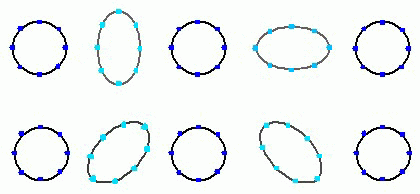
\includegraphics[scale=0.65]{Images/massesGW.png}
%\caption{Effect of passage of $+$ polarization. Image reproduced from \cite{ian}}
%\label{fig:massesplus}
%\end{minipage}
%\hspace{0.5cm}
%\begin{minipage}[b]{0.5\linewidth}
%\centering
%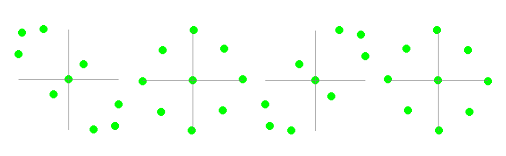
\includegraphics[scale=0.35]{Images/cross.png}
\caption{Effect of passage of $+$ polarization (top row) and effect of passage of $\times$ polarization (bottom row) through a ring of particles: the effect is of squeezing and extending along different axes for the two GW polarizations.}
\label{massesGW}
%\end{minipage}
\end{figure}

When a gravitational wave passes through the interferometer, the space--time in the local area is altered. Depending on the source of the wave and its polarization, this results in an effective change in the length of one or both of the ``L'' arms. Consider a gravitational wave detector with two equal length arms pointing along the $x$ and $y$ directions and suppose an incident gravitational wave propagating along the $z$ direction towards the detector. Knowing that light travels along null geodesics hence $\mathrm{d}s^2=0$, we can estimate the change in light time along each of the detector's arms. For the $x,~y$ axes
%
\be 0 = -c^2\mathrm{d}t^2 + (1 + h_+(t)) \mathrm{d}x^2 \ee
%
Integrating, the light time will be along the $x$ axis
%
\be \Delta t_x = t_x - t_0 = \frac{1}{c}\int_0^{L_0} \sqrt{1 + h_+} \mathrm{d}x \approx \frac{L_0}{c} + \frac{1}{2c}\int_0^{L_0} h_+ \mathrm{d}x \ee
%
where $L_0$ is the length of the arm when no gravitational wave is incident on the detector and we have ignored terms that are second order in $h_+$. The integral on the right of this equation is easily evaluated if we assume that
$h_+$ does not vary significantly during travel along the arm, therefore taken as constant. This is a fair assumption for the realistic case of an interferometer with 4km arms and a gravitational wave with 100Hz frequency. The light travel time to travel up the $x$ arm is then given by
%
\be c \Delta t_x \equiv L_x = L_0 ( 1 + h_+ ) \ee
%
Similarly the light travel time down the arm is evaluated in the same way and has the same value. The difference in the light travel time to go up each arm and back to the beam splitter is then given by
%
\be \label{eq:intro_dt_simple}
c \Delta t = c(\Delta t_x - \Delta t_y) \equiv L_x - L_y =  L_0 h \ee
%
\be \label{varh_L} h = \frac{\Delta L}{L_0} = \frac{L_x - L_y}{L_0} \ee
%
Therefore as $h$ varies, the relative length of the two arms
will also vary. This will then cause variations in the power observed at the photodetector,
allowing us to directly observe the variation in the gravitational field.

There is, however, a significant difference between this simple explanation and an actual gravitational wave interferometer designed to detect gravitational radiation with amplitudes of order $h \sim 10^{-22}$. To achieve this level of sensitivity the operation of gravitational wave interferometers is much more complex than the description here. For example, Fabry--Perot cavities are used to increase the effective path length of the laser light and allow for multiple reflexions of the beams before recombination at the photodetector (an optical cavity or resonator is an arrangement of mirrors that forms a standing wave cavity for EM waves). Power recycling techniques and high powered lasers are used to maximize the power coming out of the beam splitter. A much more comprehensive description of the operation of gravitational wave interferometers and the difficulties they have to overcome can be found in \cite{Saulson:1994,Maggiore:gw}.

\subsubsection{Detector antenna pattern functions}
Gravitational wave detectors, like many other astronomical observatories, have a limited sensitivity to source detection, depending on the location and the properties of the source. They can be described, analogously to radio antennae, by expressing their sensitivity in terms of \emph{antenna factors}.

Consider again the $x-y$ plane of the detector with its two arms along $x$--axis and $y$--axis respectively. We will call this plane the \emph{detector frame}. Consider now an incident gravitational wave $h = (h_+, ~h_{\cross})$ with its two polarizations parallel to a different plane $x'-y'$. We will call this plane the \emph{radiation frame}. This more general case when the radiation frame is not aligned with the detector frame can be easily solved by performing a series of rotations (just as we did above when transitioning from radiation frame to GW source frame). The angles relating the detector frame to the radiation frame are shown in Figure \ref{fig:intro_det_rad}. The angles $(\theta,\phi)$ give the sky location of the source relative to the detector frame. These two angles translate us to a frame in which the perpendicular $z'$ on the radiation plane points from the source to the detector. A further angle, the polarization phase, $\psi$, is needed to rotate the $x$ and $y$ axes of this frame into the radiation frame.
%
\begin{figure}[tp]
  \centering
  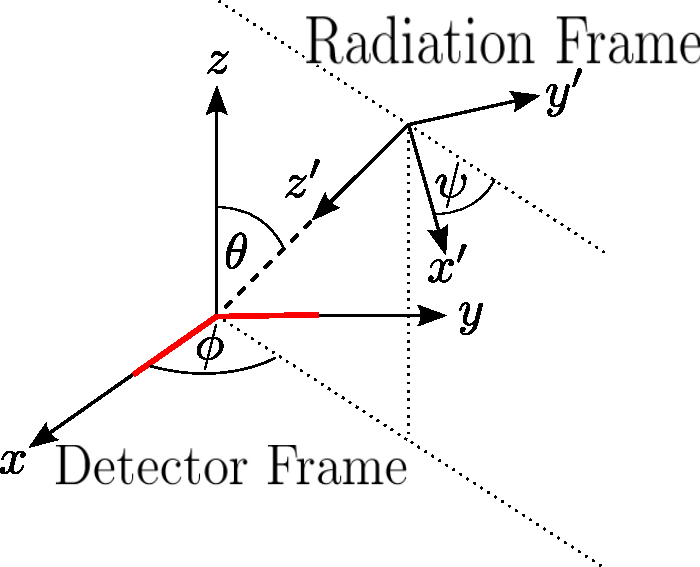
\includegraphics[width=0.5\linewidth]{Images/skyangles.pdf}
  \caption[The angles that describe the relationship between the detector
and radiation frames.]{\label{fig:intro_det_rad}
An illustration of the angles that describe the relationship between the detector
and radiation frames. Figure originally published in \cite{Mckechan:2010}.}
\end{figure}

The gravitational wave at the detector will be a linear combination of the two source polarizations
%
\be \label{eq:intro_hoft}
h(t) = F_+ h_+(t) + F_{\cross} h_{\cross}(t) \ee
%
In this expression $F_+$ and $F_{\cross}$ give the detector response to the $h_+$ and $h_{\cross}$ components respectively of the gravitational wave in the radiation frame. Explicitly these are given by \cite{Allen:2005fk}
%
\begin{subequations}
  \label{eq:fplus_fcross}
 \begin{align}
  F_+ (\theta,\phi,\psi) &= - \frac{1}{2}(1 + \cos^2\theta)\cos2\phi \cos2\psi
- \cos \theta \sin 2\phi \sin 2\psi \\
  F_{\cross} (\theta, \phi, \psi) &= \frac{1}{2}(1 + \cos^2\theta)\cos2\phi \sin2\psi
- \cos \theta \sin 2\phi \cos 2\psi
 \end{align}
\end{subequations}

The polarization angle of an incoming gravitational wave would generally be expected to be uncorrelated to its direction of arrival (polarization is related to orientations in the source). Then it is useful to characterize the  directional sensitivity of a detector by averaging over the polarization angle $\psi$. If we are interested in a single detector's response, it is always possible to align the polarization angle $\psi$ in the sky plane with that of the wave, so that the wave has pure $+$-polarization. Then the root mean square response function of the detector is 
%
\begin{equation}\label{eqn:rmsresponse}
F_{\mathrm{rms}} =  \left(\int F_+^2\mathrm{\ d}\psi \right)^{1/2}.
\end{equation}
%
The function $F_{\mathrm{rms}}$ is often simply called the \emph{antenna pattern} and for an interferometer, it is given by
%
\begin{equation}
F_{\mathrm{rms}} = \sqrt{F_+^2 + F_{\cross}^2} = \sqrt{ \frac{1}{4} \left ( 1 + \cos^2\theta \right)^2
\cos^2 2\phi + \cos^2\theta \sin^2 2\phi }
\end{equation}

\begin{figure}[ht!]
\centering
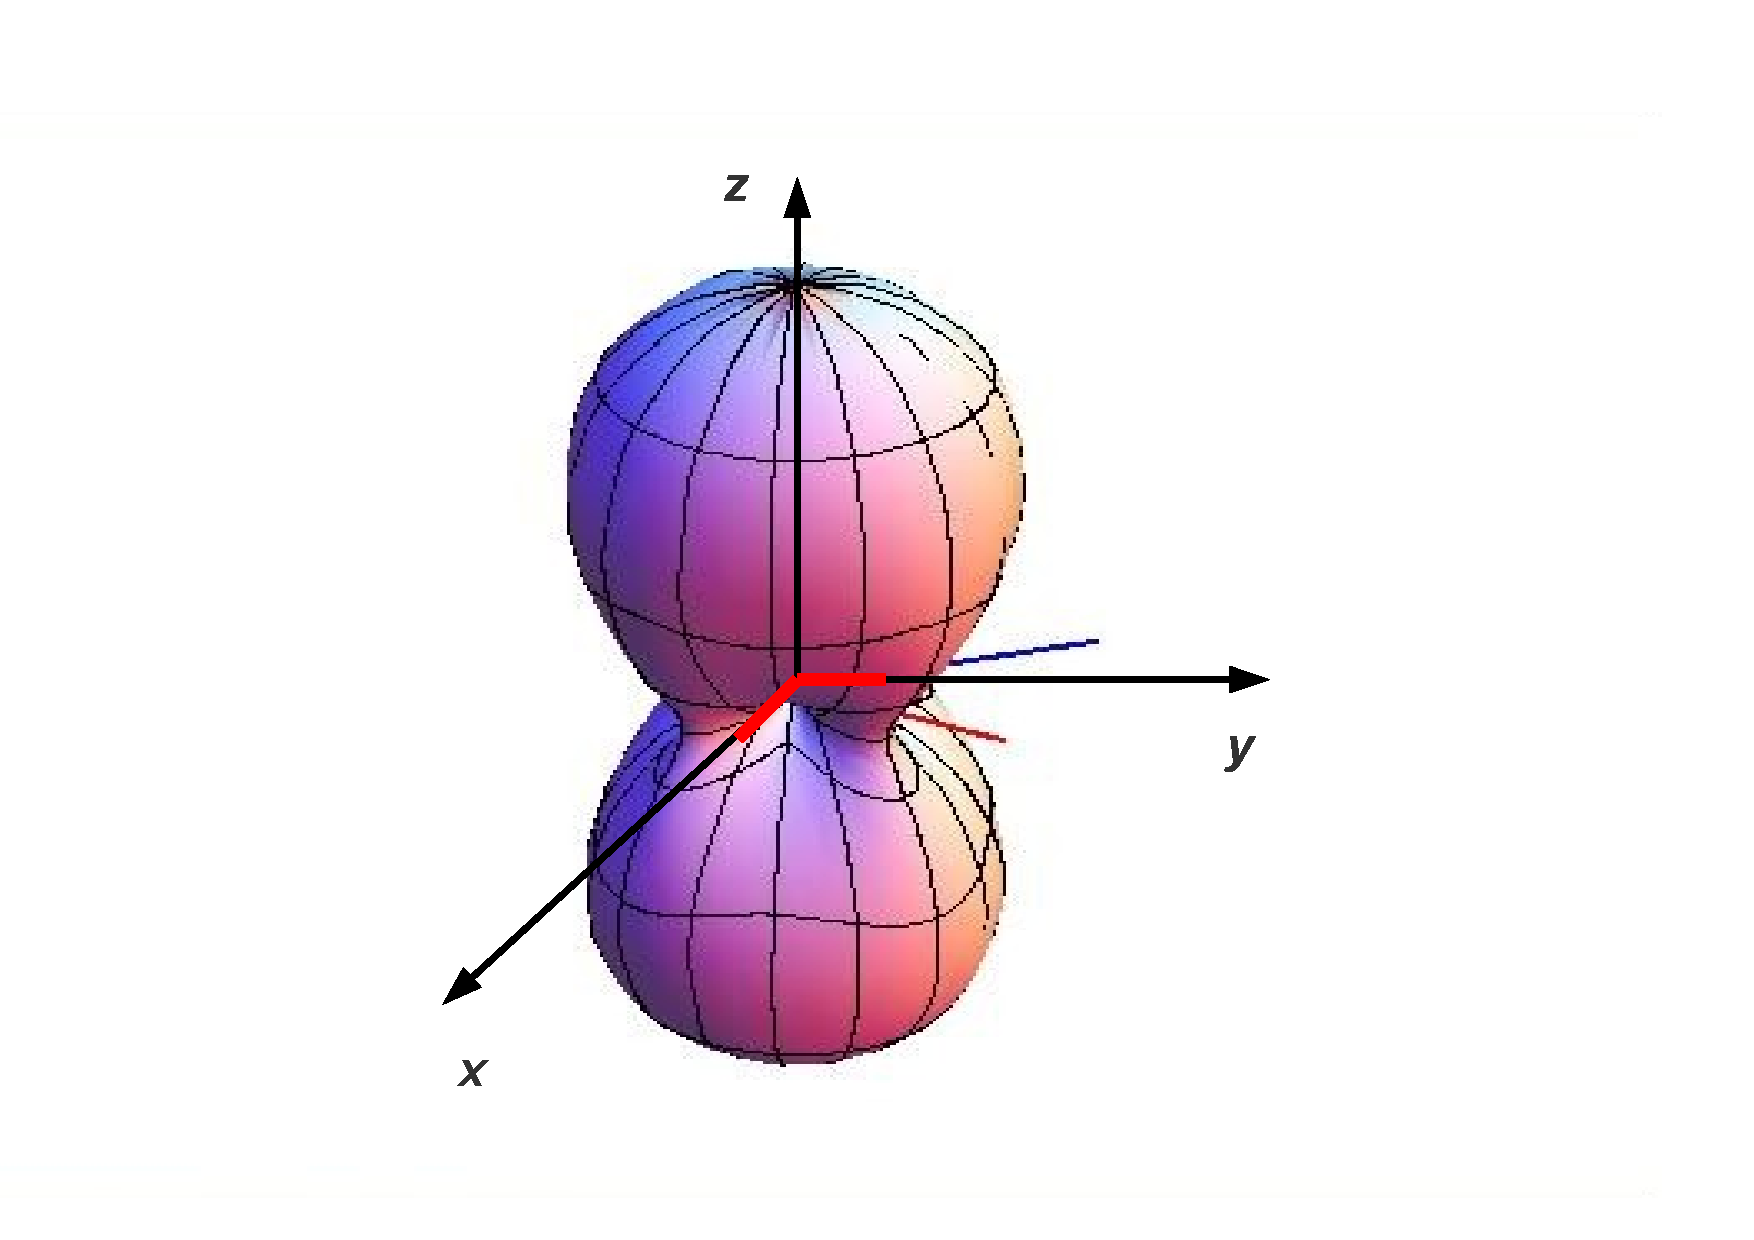
\includegraphics[scale=0.25]{Images/peanut.pdf}
\caption{A GW detector sensitivity to an unpolarized GW wave varies with the source direction -- here plotted the antenna response $F_+$ of an interferometric GW detector with the arms in the $x-y$ plane and oriented along the two axes. The response $F_+$ for waves coming from a certain direction is proportional to the distance to the point on the antenna pattern in that direction. This clearly shows the quadrupolar nature of the wave. Image reproduced and modified from ~\cite{Sathyaprakash:2009xs}}
\label{peanut}
\end{figure}

The Figure \ref{peanut} gives us an idea of how sensitive a single \ac{GW} detector can be to a gravitational wave with a certain polarization and incident from a certain direction on the sky: the response $F$ for waves coming from an arbitrary direction is proportional to the distance to the point on the antenna pattern in that direction; also this clearly shows the quadrupolar nature of the wave; a single detector has a limited capability of detecting waves with sources ``sub--optimally'' located - the ideal case would be a source directly overhead.   

\subsubsection{A CBC $h(\tau)$ at the detector}
We wish to calculate the strain that would be observed at a gravitational
wave detector due to the passage of a gravitational wave emitted by a \ac{CBC}.
To do this the expressions for $h_+(t)$ and $h_{\cross}(t)$ can be combined
with equations (\ref{eq:intro_hoft})
and (\ref{eq:fplus_fcross}) as follows:
%
\begin{subequations}
\begin{align}
h(\tau) =& F_+ h_+(\tau) + F_{\cross} h_{\cross}(\tau) \\
     =& \left(- \frac{1}{2}(1 + \cos^2\theta)\cos2\phi \cos2\psi
- \cos \theta \sin 2\phi \sin 2\psi\right) \nonumber \\
& \left(\frac{2}{D} \mathcal{M}^{5/3}
\left( \pi f(\tau) \right)^{2/3}
\left( 1 + \cos^2 \iota \right)
\cos \left(
\Phi(\tau)+ 2\varphi\right) \right) \nonumber \\
    &+ \left(\frac{1}{2}(1 + \cos^2\theta)\cos2\phi \sin2\psi
- \cos \theta \sin 2\phi \cos 2\psi\right) \nonumber \\
& \left(-\frac{2}{D} \mathcal{M}^{5/3}
\left( \pi f(\tau) \right)^{2/3}
(2\cos \iota) \sin \left(
\Phi(\tau)+ 2\varphi\right)\right). \nonumber
\end{align}
\end{subequations}
%
Re--writing these as harmonic functions with an amplitude and a phase term:
%
\be
\label{eq:h_amp_phase}
  h(\tau) = A(D,\iota,\theta,\psi,\phi)\mathcal{M}^{5/3}\left( f(\tau) \right)^{2/3} \cos\left(\Phi(\mathcal{M},\tau)
+ \Phi_0 (\iota,\varphi,\theta,\psi,\phi) \right),
\ee
%
where $A$ is a constant amplitude term and $\Phi_0$ a constant phase offset. Or equivalently
in the frequency domain as
%
\be
\label{eq:h_amp_phase_freq}
\tilde{h}(f) = \tilde{A}(D,\iota,\theta,\psi,\phi) \mathcal{M}^{5/6}f^{-7/6}
\exp\left[i\left(\Phi(\mathcal{M},f) + \tilde{\Phi}_0 (\iota,\varphi,\theta,\psi,\phi,t_c) \right)\right],
\ee
%
This shows that a single detector can only distinguish an amplitude and a phase for the incident \ac{GW} and it would not be possible to extract information on sky localization and distance to the source since amplitude and phase are degenerate. However, if more than one detector is used, the degeneracy can be broken and these parameters can be recovered. We note that if the phase evolution is evaluated to higher
order it will depend on $\eta$ as well as $\mathcal{M}$ and time/frequency.

\subsection{Gravitational radiation from a binary neutron star merger}
\label{sec:cbc_example}

It is useful to consider a practical example of a binary neutron star merger, using the theoretical derivations we have have done in the previous sections. Consider a compact binary neutron star inspiral, with both components approximated to point--like masses having typical neutron star masses of $m_1 = m_2 = 1.4M_{\odot}$. Let this system be located at a distance of $D=1~\mathrm{Mpc}$ and ideally directly over a detector hence $\theta=\phi=0$. Additionally, let it be ideally oriented such that $\iota = \varphi = \psi = 0$. The gravitational waveform at the detector, in such a case, would have the expression from equation (\ref{eq:h_amp_phase}) in SI units:

\begin{equation}
h(\tau) = \frac{1}{D} A(\iota,\theta,\psi,\phi) \mathcal{M}^{5/3}f^{2/3} \mathrm{e}^{i\left(\Phi(\mathcal{M},f) + \tilde{\Phi}_0 \right)}
\end{equation}
%
where

\be
A(\iota=0,\theta=0,\psi=0,\phi=0) = \frac{4 \pi^{2/3} \left( G \mathcal{M} \right)^{5/3}}{c^4}
\ee
%
and using equation (\ref{eq:omegatau}) we obtain the expression $h(\tau)$:

\begin{equation}
h(\tau) = \frac{1}{D} \left( \frac{G \mathcal{M}}{c^2} \right)^{5/4} \left( \frac{5}{c \tau} \right)^{1/4} \mathrm{e}^{i\left(\Phi(\mathcal{M},\tau) + \Phi_0 \right)}
\end{equation}
%
Plugging in the numbers for $\mathcal{M} = 1.21 ~M_{\odot}$ and $D=1~\mathrm{Mpc}$ we obtain an amplitude 
%
\be
A(\tau) \approx \frac{10^{-21}}{\tau^{1/4}}
\ee
%
The gravitational waveform that this system would produce in the detector is shown, in the time domain, in Figure \ref{chirpwaveT} and is the ``chirp--wave''. This also shows the order of magnitude of the strain we expect to detect from a binary neutron star coalescence at a reference distance $D=1~\mathrm{Mpc}$ and ideal orientation and localization, $h(\tau) \approx 10^{-21} / \tau^{1/4}$.

\begin{figure}[ht]
\centering
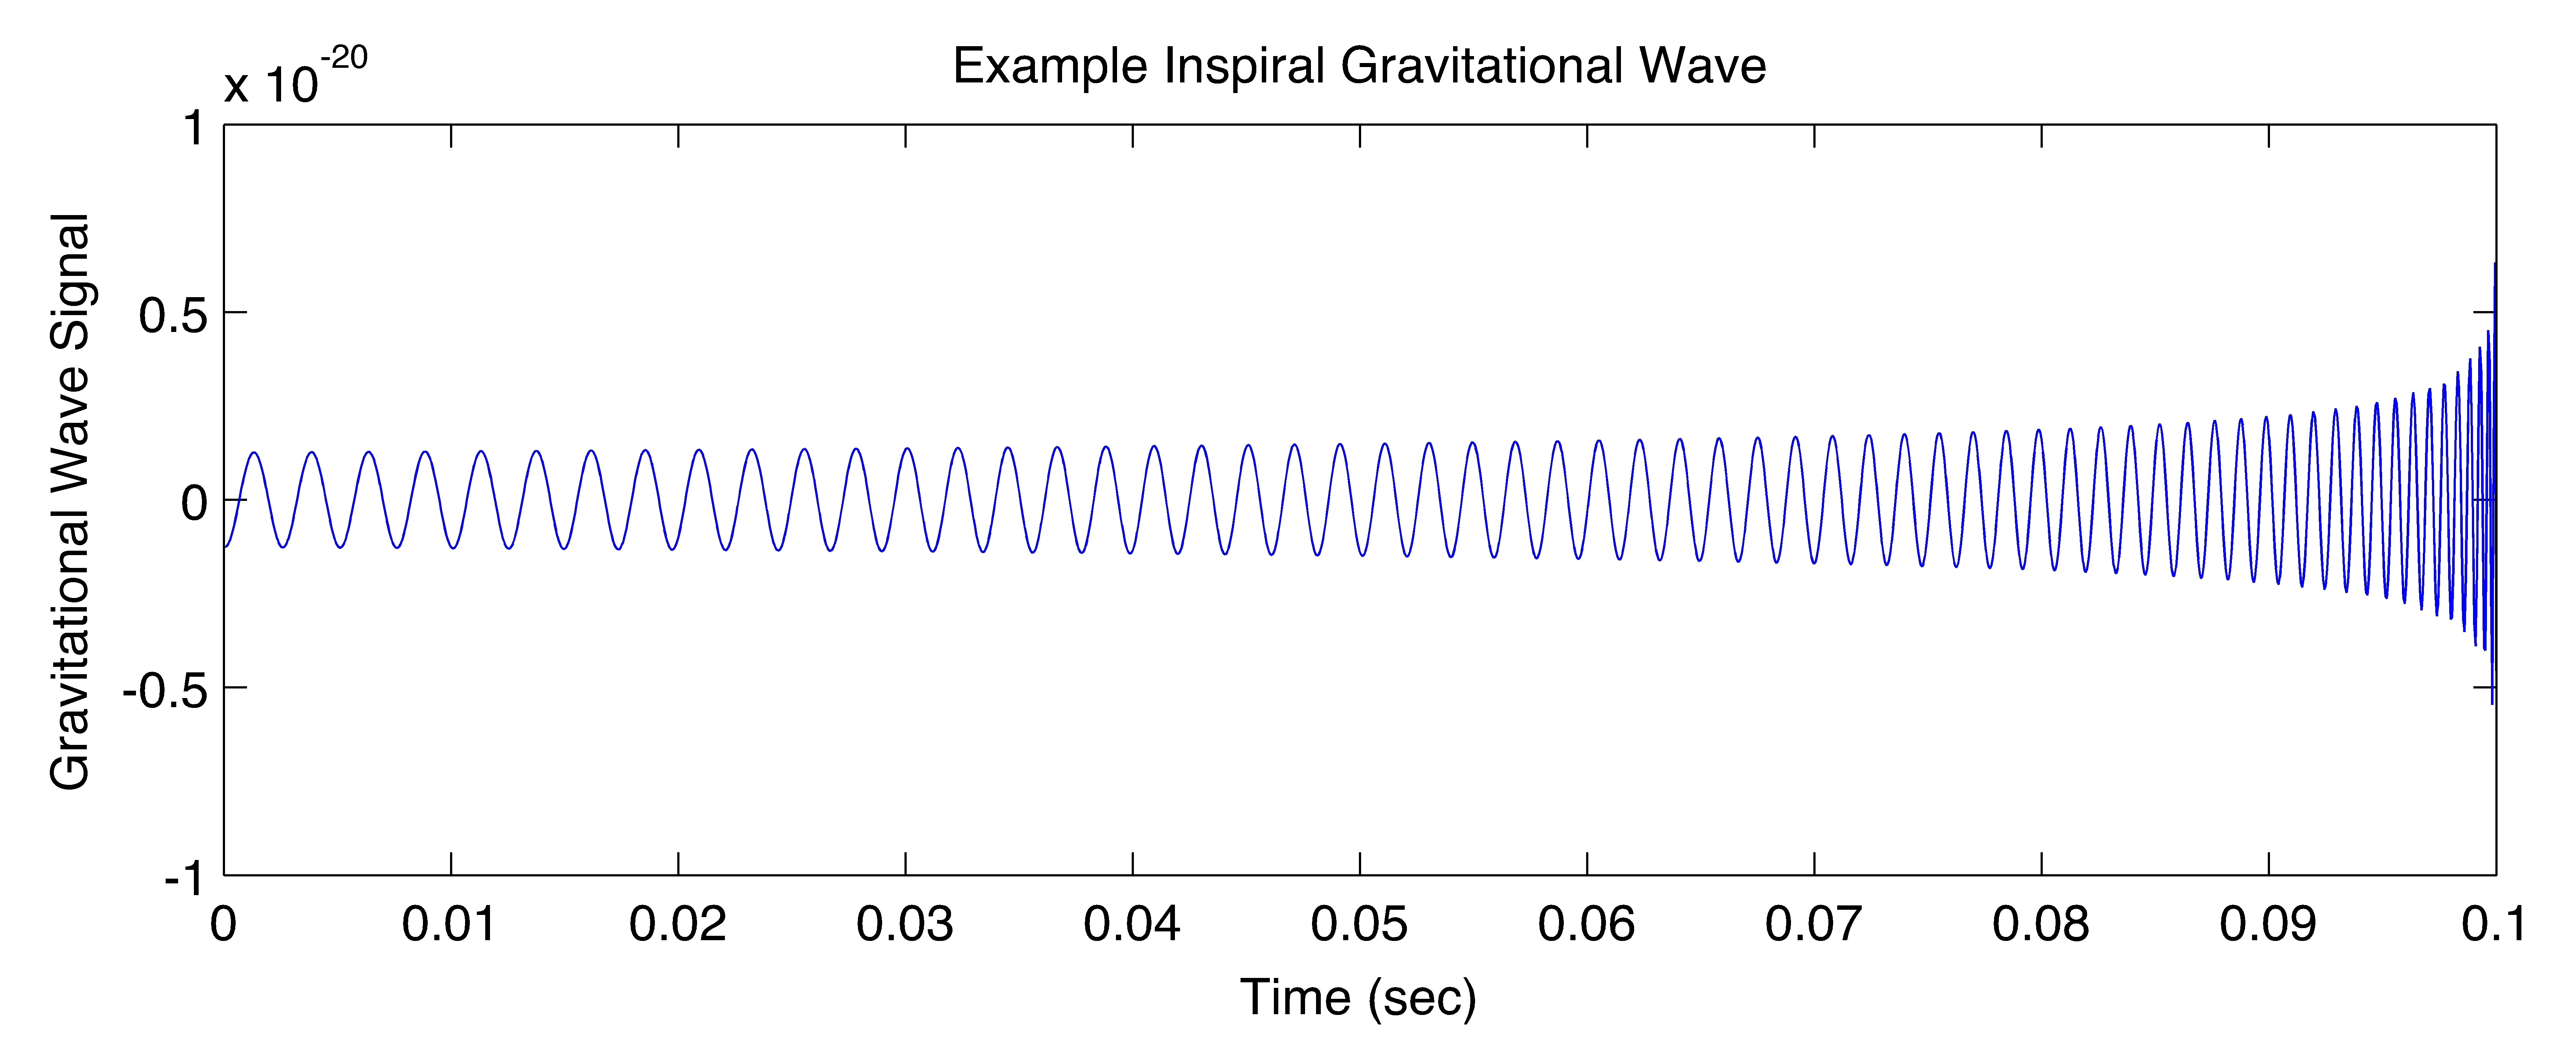
\includegraphics[scale=0.05]{Images/chirpT.png}
\caption{Time evolution of the strain $h(\tau)$ at the detector due to a \ac{GW} -- the ``chirp'' wave in time domain. This particular ``chirp'' is produced to first order by an ideally located and oriented CBC with equal masses and no spins.}
\label{chirpwaveT}
\end{figure}

In the analysis it is useful to write the waveform at the detector as:
\be h(\tau) = \frac{1 ~\mathrm{Mpc}}{D_{\mathrm{eff}}}\left(h_+\sin \left(\Phi(\tau)+ 2\varphi\right) + h_{\cross}\cos \left(\Phi(\tau)+ 2\varphi\right)\right)
\ee
%
where 

\be
D_{\mathrm{eff}} = \frac{D}{\sqrt{F^2_+(1+\cos^2 \iota)/4 + F^2_{\cross} \cos^2 \iota}}
\ee
%
is the effective distance to a binary given the antenna response factors $(F_+,~F_{\cross})$ and $h_+, ~h_{\cross}$ are the two polarizations for a binary ideally oriented and located.

One must remember that this waveform has only been generated to first order and without taking into account the spin of the component objects. For a real signal, higher order terms will be important close to merger. Additionally, the assumption of point masses will break down at merger, as effects due to the size of the objects, such as the tidal interaction between two neutron stars, can become noticeable.

\section{Gravitational Waves Detectors -- Practical Issues}
Suppose we consider a real gravitational wave interferometer with each of the ``L'' arms of 4 km long. The variation in ``L'' arm length to which a \ac{GW} interferometer should be sensitive in order to detect a \ac{GW} of strain amplitude $h \approx 10^{-21}$, given an arm length of 4 km follows from equation (\ref{varh_L}):

\begin{equation}
\Delta L \approx hL = 4 \times 10^{-18}~\mathrm{m}
\end{equation}

At such scales, one would expect that even the smallest amount of noise would drastically affect the sensitivity of a \ac{GW} interferometer. The time it takes light to travel along the arms is of order $10^{-5}$~s, much smaller than the duration of a gravitational wave. In order to enlarge this time, different optical components are used to keep the light longer in the arms. These optical parts will introduce their own sources of noise. Internal and external detector environment factors can contribute to both stationary and non--stationary noise effects and are briefly mentioned here.

\subsection{Stationary noise sources}

The main sources of stationary noise for a typical interferometric detector are given in various references and summarized here. For a more in--depth analysis of the topic we direct the reader to a few references, e.g., \cite{Saulson:1994, Sathyaprakash:2009xs, Blackburn:2008ah, Accadia:2010zzb, Accadia:2010zz}. Figure \ref{noisesF} shows the stationary noise contributions in the frequency regime for a GW detector.

\begin{figure}[ht!]
\centering
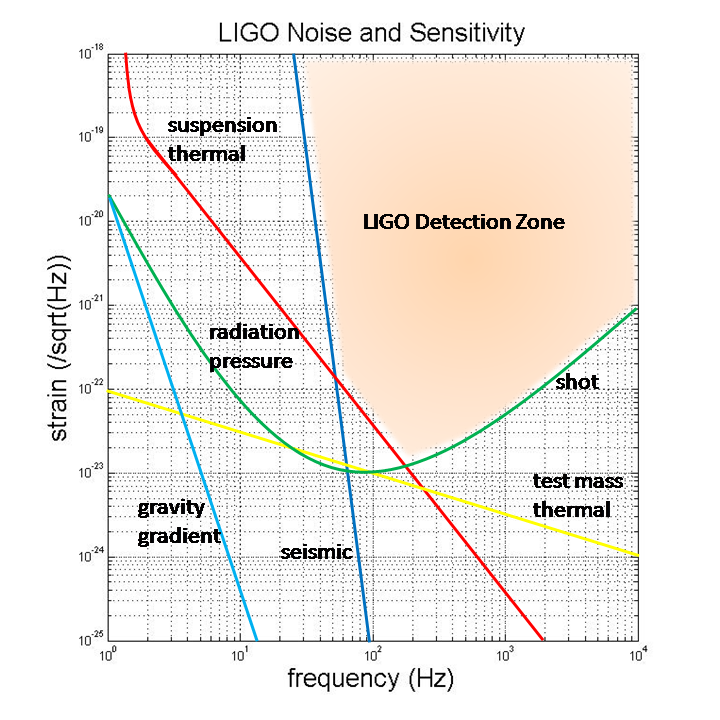
\includegraphics[scale=0.50]{Images/noisesF.png}
\caption{Different noise contributions in the frequency regime. Image from \cite{ian}.}
\label{noisesF}
\end{figure}

\begin{itemize}
 \item
   {\bf Thermal noise:} Thermal vibrations of the internal parts of the interferometer can mask gravitational waves. Interferometers minimize the effect of noise by measuring only at frequencies \emph{far} from the resonant frequency where the effects of thermal noise are maximum (suspensions have resonant frequencies of a few Hz, whereas mirrors' are at a few kHz, see Figure \ref{noisesF}). This noise source is also minimized by making sure all materials have high quality factors, which is technologically demanding, so their resonances are sharp and energy leakage to measurement frequencies is small. In terms of temperature, interferometers usually operate at room temperature. Alternatively the detector could be cryogenically cooled as proposed in the Japanese LCGT project \cite{lcgtwebsite}. For a reference on thermal noise please consult \cite{Gillespie:1993vg}.
 \item
   {\bf Shot noise:} The photons that are used for interferometry arrive with random phases at the photodetector. Therefore they introduce random fluctuations in the interference pattern that may mimic a gravitational wave signal (the photons are Poisson--distributed). The more photons one uses, henceby increasing the laser power, the smoother will be the interference signal.
  \item
  {\bf Mechanical vibration:} This source of noise is produced by internal vibrations of the mechanical components of the detector (primarily suspensions). Mechanical vibrations must be screened out; there are many different ways to do this, but all of them are very sensitive to frequency, working well down to a lowest effective frequency. The most ambitious isolation system is currently being developed for the Virgo detector.
 \item 
{\bf Radiation pressure:} Photons hitting the end mirrors exert a pressure on them proportional to the number and momentum of photons, moving it slightly and changing its optical contribution in the system. This noise source can be reduced by decreasing the power of the laser, thus reducing the number of photons and the total pressure. However, this will increase the shot noise. A balance must therefore be reached between the radiation pressure and the shot noise.
 \item
{\bf Seismic noise:} A very important source of noise in the low--frequency regime. Ground vibrations induced by seismic activity, man--made objects or even ocean waves may produce signals in the detector that look like very strong \ac{GW}. These vibrations act on the mirrors hence it is very important to isolate the mirrors as much as possible from the ground. The seismic noise will play an important role in the next generation \ac{GW} detectors that will operate at frequencies $\sim~4$ times lower than the present detectors. 
\end{itemize}

\subsection{Non--stationary noise sources}
The above list of noise sources enumerates only the stationary and \emph{predictable} sources of noise. More importantly, the non--stationary \emph{unpredictable} noise sources may induce large fluctuations in the detector output that may mimic strong \ac{GW} signals. These include any local small--time--scale disturbance produced by a noise transient, e.g., a truck passing near the detector will cause ground vibrations that will couple to mirror motion. There are a series of auxiliary channels that permanently monitor these noise sources and everytime there is excessive noise activity they will prompt the data to be discarded. Surviving non-stationary transients or ``glitches'' are often mistakenly picked up by the data analysis process as interesting events, therefore ``glitch''--rejection mechanisms are important and will be discussed in Chapters \ref{Chapter Three} and \ref{Chapter Four}.

\section{A network of gravitational waves interferometers} 
A global network of gravitational wave interferometers has now been constructed and has been taking data for the past ten years. The instruments constituting this network include the Laser Interferometry Gravitational Observatory (LIGO or, recently labelled as Initial LIGO), which operates two observatories at Hanford and Livingston in the USA \cite{Abbott:2007kv}; the French--Italian Virgo (Initial Virgo) detector based in Cascina, Italy \cite{virgo, Acernese:2006bj}; the British--German GEO600 detector, near Hannover in Germany \cite{Willke:2007zz} and the TAMA300 detector in Japan \cite{TAMA_status}. Initial LIGO and Virgo ceased their operations in 2010 and are both currently undergoing major upgrading work to become Advanced LIGO \cite{avlligowebsite, Harry:2010zz} and Advanced Virgo \cite{advvirgowebsite}, the second generation interferometric detectors with a much higher sensitivity than the initials.  The next subsections will briefly describe each of these detectors, for an in--depth analysis of their specifications and operational standards, we invite the reader to consult the listed references.  

\subsection{LIGO and Virgo detectors}

\ac{LIGO} (United States), is the largest interferometer in use as of today. LIGO operates two gravitational wave observatories (at two different sites) in unison: the LIGO Livingston Observatory in Livingston, Louisiana (L1 or LLO) and the LIGO Hanford Observatory, located near Richland, Washington (LHO, initially with two co--located and co--aligned detectors: H1 (4 km) and H2 (2 km)). These sites are separated by 3,002 km \cite{Abadie:2010px}. Each observatory supports an ``L''--shaped ultra high vacuum tube system, measuring 4 kilometers on each side. The primary interferometer at each site consists of mirrors suspended at each of the corners of the ``L''; it is known as a special Michelson interferometer in that it recycles the power. A pre--stabilized laser emits a beam of up to 35 W that passes through a beam splitter at the vertex of the ``L'' arms. There, the beam splits into two paths, one for each arm; each arm contains special cavities that store the beams and increase the effective path length by multiple reflections.

The Initial Virgo (Italy and France) is a 3 km detector located in Cascina, near Pisa, Italy. Virgo specializes in sophisticated suspensions, and the control of vibrational noise. Its goal is to observe at the lowest possible frequencies from the ground, at least partly to be able to examine as many pulsars and other neutron stars as possible.

The initial LIGO and Virgo took data in six consecutive science runs. Since the author has worked from the fifth run onwards as part of the LIGO Scientific Collaboration and Virgo Collaboration, we will try summarize the fifth and six runs only. The fifth science run was completed between November 4, 2005 and October 1, 2007 (known as S5 in LIGO/GEO and VSR1 in Virgo nomenclatures).  The detectors achieved a strain sensitivity of better than $10^{-22}/\sqrt{\mathrm{Hz}}$ at their most sensitive frequencies (around 100 Hz). This can be translated into sensitivities to various sources, for example the LIGO detectors in S5 were sensitive to optimally oriented and located binary neutron star coalescence signals to a distance of $\sim 35$ Mpc, and hundreds of Mpc for more massive compact binary mergers. For a better understanding of a detector sensitivity measure to GW inspiral signals from CBC objects, we invite the reader to consult Chapter \ref{Chapter Three}. For short--duration, narrow--band transients (bursts), such as the GW signal one may expect from core--collapse supernovae, this sensitivity corresponds to a gravitational wave energy as low as $10^{-8} M_{\odot}c^2 \sim 2 \times 10^{46}$~erg for galactic events and $0.1 M_{\odot}c^2 \sim 2 \times 10^{53}$~erg for events in the Virgo cluster at 16 Mpc.
%
\begin{figure}[ht!]
\centering
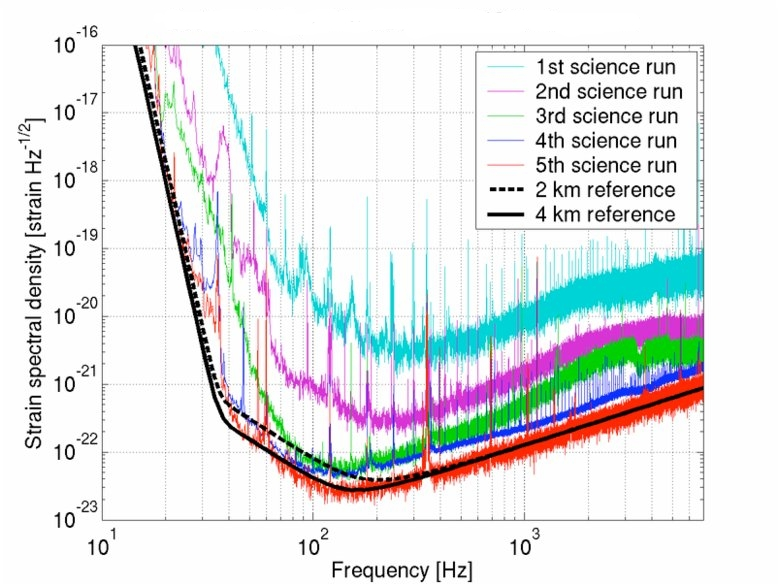
\includegraphics[scale=0.40]{Images/ligonoise.png}
\caption{LIGO noise curve for five consecutive science runs (S1 to S5): the detector sensitivity quantified by the strain spectral density is shown as function of signal frequency. The most sensitive region is around $f\sim100$ Hz. Image initially published in \cite{Abadie:2010yba}.}
\label{ligonoise}
\end{figure}

Following the S5/VSR1 run, the LIGO and Virgo detectors have been technically upgraded to enhanced configurations, and the latest completed science run was S6/VSR2 and 3 that began in the summer of 2009, and ended in fall 2010, aiming at collecting data at better sensitivities than the previous science runs (see Chapter \ref{Chapter Four}, Table \ref{tab:sciencetimes} for a complete list of dates for both S5/VSR1 and S6/VSR2 and 3).

The performance of a gravitational wave detector is characterized by the \emph{power spectral density} (or PSD) of its noise background. Although this quantity will be discussed in detail in Chapter \ref{Chapter Three}, we would like to introduce it here in light of characterizing detector sensitivity. A sensitivity curve for a detector, or a PSD curve, represents a detector strain vs. frequency plot for a frequency range for a series of noise sources. Such a curve is shown in Figure \ref{noisesF}. A collection of PSD curves for a number of GW interferometers is presented in Figure \ref{noisesmultiples}.

\begin{figure}[ht!]
\centering
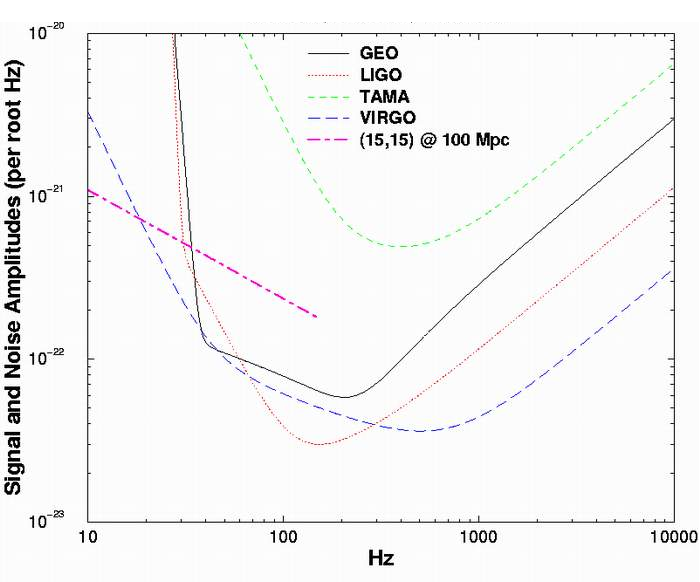
\includegraphics[scale=0.50]{Images/PSD_detectors.png}
\caption{Detector PSD curves, together with the inspiral signal evolution of a 15--15 $M_{\odot}$ compact binary at 100 Mpc. Image initially published in \cite{Abadie:2010px}}
\label{noisesmultiples}
\end{figure}

\subsection{The Advanced Detectors}

Following the initial LIGO and Virgo data taking period (S1 to S6 for LIGO and VSR1 to VSR2,3 for Virgo), both LIGO and Virgo detectors are being upgraded to advanced configurations to achieve approximately ten times the strain sensitivity (in distance) of the initial detectors. For sources distributed uniformly in volume, this corresponds to a sensitivity to a thousand times as many sources. In terms of energy, the sensitivity will be $\sim 10^{-10} M_{\odot}c^2 \sim 2 \times 10^{44}$~erg for galactic events. The low--frequency cut--off due to seismic noise will be lowered from 40 Hz to 10 Hz. The work towards completing the advanced detectors has started in 2011 and are expected to begin acquiring scientific data by no later than 2015 \cite{avlligowebsite,Harry:2010zz}.

Advanced LIGO will operate at such predicted sensitivity due to a series of radical changes from the initial detectors: the initial LIGO 10 W laser will be upgraded to a more powerful 180 W laser -- with this the input optics is changed as well, to match the new laser, improving the shot noise limited sensitivity by a factor of $\approx$ 6 with respect to Initial LIGO; the power--recycling will be more efficient as well, with changes applied to the power--recycling mirrors, resulting in a much reduced effect of thermal noise; a new suspension configuration will allow improved operation at low frequencies, where the dominant source of noise is seismic oscillations -- this way the low frequency cut--off is lowered to 10 Hz \cite{Waldman:2011vg}. 



\subsection{Sky localization with a network of \ac{GW} detectors}
\label{gw_skyloc}

Here we would like to briefly address the problem of localizing a \ac{GW} source, in case of a detection, using information from \ac{GW} detectors only. As we have seen above from equation (\ref{eq:h_amp_phase_freq}) a single detector cannot localize a \ac{GW} source. In turn, if we have two detectors, source localization could be achieved to a certain error region of the sky. \ac{GW} detectors, when working together in a \emph{network} of detectors, localize sources by \emph{triangulation} \cite{Fairhurst:2009tc}. This is possible due to differences in times of arrival of the same \ac{GW} signal at different detector sites. Indeed, if we consider two detectors (1,2) separated by a linear geographical distance ${\bf S}$ and a \ac{GW} source at a distance ${\bf R}$ on the celestial sphere, the expected time difference of signal arrival at the two detectors will be:
%
\be \Delta t_0 = t_{01} - t_{02} = \mathbf{S} \cdot \mathbf{R} \ee
%
This time delay is called the \emph{light travel time} -- the expected time difference it takes a gravitational wave to be recorded at both detector sites. We have to note that these are \emph{expected} times in the case of an ideal detector. Since the detectors are affected by noise (see Chapter \ref{Chapter Three}) the times $t_{01}, ~t_{02}$ are in reality distributed in a discrete region. \ac{GW} detectors have a relatively poor capability of determining the sky location for a source, as compared with, for example, other \ac{EM} telescopes: the angular resolution of the source can extend to thousands of square degrees; with three or more detectors the resolution will decrease to a few square degrees \cite{Fairhurst:2009tc, Fairhurst:2010is}.



\chapter{Astrophysically Triggered Searches for Gravitational Waves} % Write in your own chapter title
\label{Chapter Two}
%\lhead{Chapter~\ref{ChapterLabel}
% \emph{Astrophysically Triggered Searches for Gravitational Waves}} % Write in your own chapter title to set the page header

\section{Introduction}

Many potential sources of transient \ac{GW} signals will emit electromagnetic counterparts detectable by existing and planned astronomical instruments (see \cite{Centrella:2011nh, Metzger:2011bv, Predoi:2009af} and references therein). The coincident detection of an \ac{EM} signal would provide some of the most compelling evidence for the unambiguous direct detection of \ac{GW}, as well as provide important information on the nature of the progenitor system.

An \emph{externally triggered} \ac{GW} search represents following-up in \ac{GW} data an \ac{EM} transient, provided some information on the transient is known \emph{a priori} from astronomical observations, e.g., sky--location and time. In the next chapters I will focus mainly on the importance of analyzing \ac{GW} data around \ac{EM} events that are used as \emph{triggers} and I will describe such searches that have already been completed and others that are planned.

Searches for \ac{GW} which are \emph{triggered} by \ac{EM} observations possess several advantages over un--triggered all--sky searches. Typically, an all--sky search is performed over an entire science run, lasting months to years, and must search all sky locations for putative \ac{GW} signals. An electromagnetically--triggered search, by contrast, is usually performed over a much shorter time window lasting a few to several hundred seconds, depending on the nature of the trigger, and the sky--location of the source is usually also known to a certain degree of precision. The smaller time window increases the search sensitivity since there will be a smaller number of instrumental and terrestrial artefacts in the GW data, allowing one to identify and accept signal detections with lower significance than would be the case for a longer duration search \cite{Harry:2010fr}, see also Chapter \ref{Chapter Four}.  Knowledge of the expected time of the \ac{GW} signal allows one to make a distinction between \emph{on--} and \emph{off--source} data.  The off--source data, typically taken soon before and soon after the trigger, is used to estimate the background rate of potential gravitational wave triggers and the statistical significance of detection candidates in the on--source data, given the assumption that no GW signals from the specific EM source are to be found in the off--source (for a study of the background estimation and statistical significance of candidates see Chapter \ref{Chapter Five}). Since the noise from \ac{GW} detectors is generally non--stationary, it is important that the data used for background estimation is taken near to the trigger to accurately reflect the noise properties of the on--source data. This, however, is generally not problematic due to the fairly short on--source windows used in externally triggered analyses.  As well as the gain in sensitivity from the short on--source window, the sky--location used in electromagnetically triggered searches provides more robust signal--consistency tests in multi--detector searches and significantly reduces the parameter space of the signal, see \cite{Harry:2010fr} and Chapter \ref{Chapter Five} for a more detailed description.

Compact binary coalescence (\ac{CBC}) events are ideal source candidates for both \ac{GW} and \ac{EM} emission and the next chapters will focus on the detectability of \ac{GW} signals from \ac{CBC} events with an \ac{EM} trigger. \ac{GW} waveforms from \ac{CBC} events can be modelled theoretically and, if a detection is made, this gives an advantage over an un--modelled \ac{GW} search. By assembling a full picture of the binary parameters, using both \ac{GW} and \ac{EM} information, will lift parameter degeneracies inherent to a single \ac{GW} or \ac{EM} search \cite{Holz:2002cn, Chernoff:1993th}. Parameters such as binary luminosity distances and inclinations can be obtained from \ac{GW} search results \cite{Veitch:2009hd}. By combining \ac{GW} measurements with cosmological information, one can study the evolution of binary masses and merger rates as a function of redshift and possibly constrain merger scenarios. Second, given an associated \ac{EM} counterpart with a coalescence, it may be possible to measure both redshift and a calibration--free luminosity distance to such an event from the \ac{EM} information (spectra, dispersion measure etc.) thereby setting the energy scale and allowing an independent measurement of the Hubble constant or other cosmological parameters.

There is a series of properties that an \ac{EM} event should possess to be used as an ideal trigger for an externally triggered \ac{GW} search from a \ac{CBC} \cite{Metzger:2011bv}, namely: 
\begin{itemize}
\item
It should be detectable with present or upcoming telescope facilities -- this is necessary to ensure that systematic \ac{EM} surveys indeed take place over large times and follow--up in \ac{GW} data can be done for as many \ac{EM} events as possible, given the frequent gaps in \ac{GW} data due to poor data quality; 
\item
It should be unambiguously identifiable, such that it can be distinguished from other astrophysical transients -- this is necessary to make the association with high confidence and hence to avoid contamination from more common transient sources (e.g., supernovae, gamma--ray flares). This aspect relies heavily on the theoretical models put forward to explain the \ac{EM} transient and its origins; 
\item
it should allow for a precise determination of the sky location -- this is essential on one hand, to identifying the host galaxy and hence the redshift, as well as other relevant properties (e.g., association with specific stellar populations) and on the other hand, to minimize the sky region where the GW follow--up search will be conducted hence increasing its sensitivity. 
\end{itemize}

Short, hard gamma-ray bursts (SHB) provide a typical example of such an ideal \ac{EM} event. Constantly monitored with space--based missions, \ac{SHB} are widely believed to be the electromagnetic signatures of the coalescence of a compact binary system, consisting of two neutron stars or a neutron star--black hole and allow for a precise localization of the burst. Gamma--ray bursts have been used to trigger GW searches for some time \cite{Abbott:2007rh,Collaboration:2009kk,0264-9381-25-22-225001} and, indeed, two recent searches for GW from two \ac{SHB} whose localizations overlapped the error regions of M31 Andromeda galaxy (GRB070201, \cite{Ofek:2007th}) and M81/M82 galaxy group (GRB051103, \cite{Ofek:2006pr}) respectively, were able to confidently exclude a compact binary coalescence at the distance of M31 and M81/M82 due to the absence of significant GW emission \cite{Abbott:2007rh}. These searches did not, however, exclude a binary coalescence event at larger distances. Besides SHB, other EM transient events may play an important part in the future analyses, such as radio signatures of merging compact binaries, described in this chapter, Section \ref{section:radio}.

\section{Short Hard Gamma Ray Bursts}

Gamma-ray bursts are among the most energetic \ac{EM} phenomena in the Universe. Gamma-ray bursts were first discovered by accident at the end of the 1960's by the American Vela military mission, deployed to monitor Soviet nuclear tests. Although theories about their origin have been immediately put forward, it took almost thirty years to establish the extragalactic nature of \ac{GRB} by observing the first afterglow of a \ac{GRB} -- GRB970228 \cite{Costa:1997ji}. 

Gamma-ray bursts fall into two commonly accepted morphological groups depending on their characteristic duration of the prompt burst and spectral hardness \cite{Nakar:2007, Qinx:2010kp, Kouveliotou:1993yx, Gehrels:2006tk, Nemiroff:1993vi}, see Figure \ref{GRB_short_long}. Characteristic duration is quantitatively expressed by the $T_{90}$ parameter, defined as the time interval over which 90$\%$ of the total background--subtracted counts are observed (the total counts emitted by the source, found from the counts in the source region minus the contribution from the background), with the interval starting when 5$\%$ of the total counts have been observed \cite{McBreen:2001fd}. The majority of bursts, with softer spectrum and duration $T_{90} > \mathrm{2s.}$ are called long GRBs. They are associated with core--collapse supernova events and have been observed in optical, radio and X--ray wavelengths \cite{Campana:2006qe,Galama:1998ea,Hjorth:2003jt,Malesani:2004sg}.

\begin{figure}
\centering
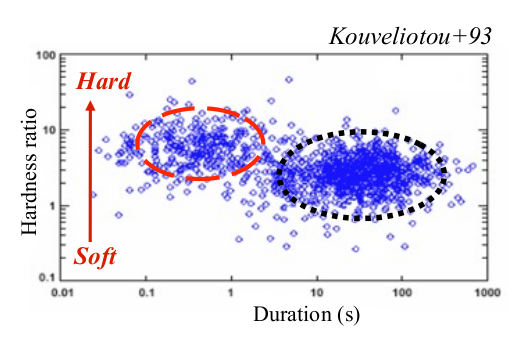
\includegraphics[scale=0.80]{Images/GRB_short_long.png}
\caption{Distribution of gamma-ray bursts in a spectrum hardness vs. duration space. The commonly--accepted ``short hard'' bursts, thought to be produced by compact binary mergers, populate the harder part of the spectrum and have shorter durations whereas the longer, softer--spectrum, unambiguously associated with stellar supernovae events, populate the lower hardness region; however, there is a region of overlap and these bursts are considered ``intermediate'' GRBs, with longer durations than SHBs, and sharing properties with the long bursts, but some with no SNe association \cite{Postigo:2010ij}. Image reproduced from \cite{Nemiroff:1993vi} for Burst And Transient Source Experiment (BATSE) bursts sample.}
\label{GRB_short_long}
\end{figure}

Those with a harder spectrum and $T_{90} \leq \mathrm{2~s}$ are labeled short hard GRBs (\ac{SHB}) and are thought to be produced by mergers of compact binaries, either binary neutron stars or neutron star-black hole. These events are ideal sources for strong gravitational wave emission \cite{ACST94, Kiuchi:2010ze}. Although the $T_{90}$ discriminator is a widely--accepted method of discerning two different classes of gamma--ray bursts, it is not a decisive indicator: e.g., recent studies have revealed the existence of an \emph{intermediate} class of \ac{GRB}, longer in duration than the typical \ac{SHB} but with the same spectral properties \cite{Veres:2010yf, Ripa:2009xs, Norris:2011tt}. It is thus important to have a full analysis of the \ac{GRB} \emph{light curves} to be able to establish its ``long'' or ``short'' nature. 

If an observation of both gamma-rays and GW originating from the same event could be achieved, it will increase confidence and allow for better science output. It is thus of great importance to constantly monitor and record SHB to allow a GW search to be performed around their burst times. Systematic analyses of GW data around short GRB times have been done in the past and the most recent publications from the LIGO--Virgo group contain results from the \emph{Swift}--observed GRBs during LIGO's fifth science run (S5) and Virgo's first science run (VSR1) \cite{Abadie:2010uf, Collaboration:2009kk} and in publication process at the time of this writing, the bursts observed by both \emph{Swift} and Fermi--GBM during S6 and VSR2 and 3, \cite{lvc:s6grb}. The analysis of the gamma--ray bursts during LIGO S6 and Virgo VSR2--3 has finished and the publication will follow soon. Another in--progress analysis effort is using GRB triggers from bursts detected by the InterPlanetary Network (IPN) and is presented in Chapters \ref{Chapter Six} and \ref{Chapter Seven}, with short--term publication plans. This effort is led by the author of this thesis.

\subsection{SHB progenitors, their host galaxies and local rates}

\paragraph{SHB progenitors}
Short GRBs ($T_{90} \leq \mathrm{2s.}$) are amongst the brightest cosmological sources of EM radiation in the Universe, with energies of $\sim~10^{48}-10^{52}$ ~erg \cite{Nakar:2007,Berger:2010qx}. Given the short duration and spectral hardness, their progenitors are widely believed to be mergers of \emph{compact} objects, either neutron star--neutron star (NS--NS) or neutron star--black hole (NS--BH) binaries \cite{Paczynski:1986px, Nakar:2007, Belczynski:2006br, Troja:2007kt, Metzger:2011bv, Capozziello:2010sm, Berger:2010qx} (and references therein). There is no conclusive observational evidence supporting this case, therefore in the next paragraphs we will mainly list a series of short hard GRB properties that differentiate them from the long soft GRB population, in an indirect way of motivating a compact binary merger progenitor model for them.

A good indicator of their progenitor would be securing a host galaxy for each burst, preferably with very low or extinct star formation, the most likely host for compact binary mergers formed at the peak of the galactic star forming period \cite{Kelley:2010qx}. A host galaxy can be identified by observing an \ac{SHB} afterglow, localized to sub--arcsecond precision; usually, an X-ray afterglow is observed first, that will trigger an optical follow--up with results of sub--arcsecond precisions. Although some \ac{SHB} afterglows have been observed in different wavelengths, short hard GRBs are known for weak afterglows, making it difficult to obtain a large enough sample for unambiguous statements. Prior to 2005, when the first optical and X-ray afterglows of SHB were detected, the compact binary progenitor model had been a viable theoretical explanation of the energetics and emission mechanism of such bursts with no observational support. After the first afterglows of SHB have been detected (e.g., GRB050509B, GRB050709 and GRB050724, \cite{Pedersen:2005kh, Nakar:2007xe}), a few important observations have been made to partially support the compact binary merger progenitor model and partially to prove that the SHB origins differ from long GRB's. First, their X-ray and optical afterglow spectra could not be associated with core--collapse supernovae (the observationally confirmed progenitor of long GRB \cite{Woosley:2006fn}). Second, based on afterglow observations, most of the hosts are identified to be star--forming galaxies (ratio 4:1 to old galaxies \cite{Berger:2010qx}) but with lower star formation rate (SFR) and higher metallicity than the hosts of long bursts \cite{Berger:2010qx}; a few hosts have been identified as old elliptical with almost null SFR. 

For the few SHB that have confirmed redshifts to date, their redshift distribution is inconsistent with a bursting rate that traces the SFR in the universe, unlike long--soft GRBs, which do follow it \cite{Prochaska:2005qf}. The association with low(er)--SFR galaxies and their position within these galaxies support an old ($\sim$~Gyr) progenitor, like NS--NS or NS--BH binaries.

Another argument in support of the compact binary coalescence progenitor model for \ac{SHB} is the redshift--luminosity two--dimensional distribution \cite{Nakar:2007}. The SFR is higher at larger redshifts ($z \geq 1$) and a lot of the \ac{SHB} are observed at lower redshifts ($z \geq 0.3$) -- this implies that the progenitors are born when the Universe is still young and produce the \ac{SHB} at a much later stage, explaining time differences of $\sim$Gyr, hence old compact binaries.

One recent proposal put forward to distinguish short hard from long soft--spectrum bursts is the still controversial so--called ``Amati relation'' between the peak energy in gamma-rays ($E_p$) and the isotropic equivalent radiated energy ($E_{\gamma, \mathrm{ISO}}$) for bursts with known redshift \cite{Amati:2002ny}. This empirical relation states that $E_p \propto E_{\gamma, \mathrm{ISO}}^{0.5}$ for long soft bursts and the short bursts do not follow this proportionality relation (are outliers). There is, however, a wide spread in the data distribution and the instrumental effects are still unclear, to identify this as a definitive argument in differentiating short from long bursts.

Consider now that we accept the compact binary merger progenitor model for SHB; we would want to differentiate the binary NS or the NS--BH types of mergers. Due to a relatively small number of SHB afterglow observations, and if SHB are truly compact binary merger events, it is still unclear what proportion of the bursts are produced by either NS--NS or NS--BH mergers. A few models have been put forward trying to relate the progenitor nature with its environment.

Based on burst durations and X-ray afterglow extended emission, measured redshifts and locations for a sample of SHB, according to \cite{Troja:2007kt}, SHB with measured offsets from host galaxies appear qualitatively divided into two groups. The group with larger $T_{90}$ durations and afterglow extended emission all lie very close to their hosts, favoring an NS--BH merger progenitor (this, supported by two arguments: the BH might not have received an energetic ``kick'' at its birth \cite{Mirabel:2003st} and the merger times for NS--BH systems are of order 100 shorter for a $1.4 - 14 M_{\odot}$ system), while the group with shorter durations and no extended emission have a mean offset of factor $\sim$~15 larger, favoring an NS--NS merger as progenitor. 

There is also variety in characteristic ages of the binaries that are thought to produce the SHB -- reference \cite{Belczynski:2006br}, based on the known Galactic binary pulsars and using a population synthesis model, infers that there are two classes of binaries -- ones with old ages of $\sim$~0.1-15 Gyr before merging (80$\%$ chances to be NS--BH) and others with much shorter ages of $\sim$~0.001--0.2 Myr (equally probable to be NS--NS and NS--BH). This leads to a possible association with host galaxies: for starburst galaxies (which on average have small masses) where stellar populations are young, mergers from short--lived double compact objects are expected; in elliptical galaxies, with a very low SFR, mergers of long--lived double compact objects are expected.

Although binary coalescence is the favored progenitor model for short GRBs, this has not yet been confirmed by means of a direct observation and some other progenitor models have been put forward as alternatives, for instance reference  \cite{MNR:MNR12923} proposes that SHB may originate from double white dwarf mergers. Consequently, the detection of gravitational waves associated with a short GRB would provide evidence that the progenitor is indeed a coalescing compact binary and also provide information on the parameters of the binary (most importantly the masses for NS--NS and masses and spins for the NS--BH case).

\paragraph{Binary merger rates}
\label{shbrates}
Unfortunately, actual observational constraints on compact binary populations may be obtained only for NS--NS systems since only such binaries are currently directly observed as binary pulsars (e.g., the three known systems: Hulse-Taylor PSR B1913+16, B1534+12, and J0737-3039 \cite{Kim:2006fm}, also described in Chapter \ref{Chapter One}). Merger rates extrapolated from the observed sample of Galactic relativistic NS--NS binaries have been presented in \cite{Nutzman:2004bw,Kim:2006fm} (and references therein). 

Based on the number of galactic binary pulsars, according to \cite{Nutzman:2004bw} the best estimate of the NS--NS merger rate in the Galaxy is presently $\sim 10^{-5}-3 \times 10^{-3}~\mathrm{yr}^{-1}$. All extrapolations from Galactic to extragalactic rates are based on the assumption that the formation of binary compact objects in a region is proportional to the blue luminosity in that region, corrected for reddening \cite{Phinney:1991ei}. Based on this, the rates convert to $\sim 2 \times 10^2-3 \times 10^3~\mathrm{Gpc}^{-3}\mathrm{yr}^{-1}$ for a galaxy number density of $10^{-2}~\mathrm {Mpc}^{-3}$. This would imply a LIGO/Virgo rate of $\sim 5 \times 10^{-3}-0.1  ~\mathrm{yr}^{-1}$ for the present detectors. More recently, and again based on the known binary pulsars, according to \cite{Kim:2006fm}, the NS--NS merger rate within the Galaxy should be in the range $\sim ~10^{-6}-1.5 \times 10^{-4} ~\mathrm{yr}^{-1}$ implying LIGO/Virgo event rates in the range $\sim ~4 \times 10^{-4}-6 \times 10^{-2} ~\mathrm{yr}^{-1}$ for the present detectors and $\sim ~2-330 ~\mathrm{yr}^{-1}$ for the advanced detectors.

In \cite{Nakar:2007} the range for the volume rates for short hard GRBs considered compact binary mergers, at redshift null and detectable with present gamma-ray telescopes are estimated to $\sim ~10-10^4 ~\mathrm{Gpc}^{-3}\mathrm{yr}^{-1}$ which would imply a detection rate of $7 \times 10^{-4} - 7 \times 10^{-1} ~\mathrm{yr}^{-1}$ for the present LIGO/Virgo, assuming a naive uniform volume distribution of SHB events (justified by an isotropic distribution of long and short bursts, observed by BATSE). These rates are consistent with the expected binary neutron star merger rates.

\subsection{Emission mechanism}
\label{SHBmodel}

The coalescence of a compact stellar-mass binary (either two neutron stars or a neutron star and a black hole companion) is the endpoint of its (presumed) $\sim$ Gyr life revolving around the common center of mass while constantly losing energy and angular momentum through emission of gravitational radiation. The binary merger will lead to the formation of either a transient hyper-massive highly magnetized neutron star with a lifetime of a few ms \cite{Shibata:2005mz, Duez:2005cj} that will collapse to a rapidly spinning black hole or straight to the formation of a black hole \cite{ShibTan06, Shibata:2007zm}. In the favored model of short GRBs \cite{Shibata:2005mz, Kiuchi:2010ze, Rezzolla:2011da, Oechslin:2005mw}, the gamma-ray emission is contingent on the formation of a massive (and highly magnetized) torus around the final black hole. The matter in the torus is accelerated to relativistic velocities leading to the formation of a collimated jet of electromagnetic radiation along the axis of the former binary total angular momentum. Differences in velocities between layers in the jet account for the prompt gamma-ray emission.

\paragraph{GW--gamma-ray emission time difference}
A critical parameter in searching for GW associated with SHB is the difference in the burst/GW arrival times at the Earth. Several semianalytical calculations of the final stages of a NS--BH inspiral show that the majority of matter plunges onto the BH within order 1s \cite{Davies:2005}. Full relativistic and magnetohydrodynamic numerical simulations have shown that the time difference between the binary merger and the jet formation can be between a few milliseconds up to a few seconds \cite{ShibTan06, Shibata:2007zm, Rezzolla:2011da, Rezzolla:2010fd, Baiotti:2008ra, Oechslin:2005mw}.

\begin{figure}
\centering
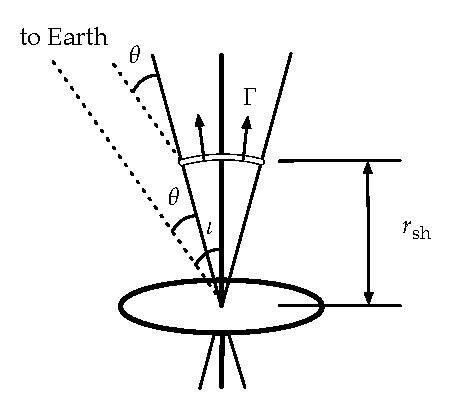
\includegraphics{Images/CBC_geometry}
\caption[Geometry of the compact binary coalescence model of short GRBs]
{Geometry of the compact binary coalescence model for short hard gamma-ray bursts.
Parameters are: $r_\mathrm{sh}$ is the distance between the central engine and the inner
shock, $\iota$ is the inclination angle, which is the angle between the
line of sight of an Earth--based observer and the orbital axis.
Although we generally believe that Earth is within the jet opening angle,
we depict the angle $\theta$ between our line of sight with the engine
and our line of sight with the nearest outflow direction for generality. This choice of angles makes the distinction between the outflow half--opening angle (the jet angle, $\iota - \theta$) and the observed inclination angle -- there might be the case that a GRB is observed after a jet break. In the cases we will follow further on, we will assume that the observer is placed within the jet cone, reducing to $\theta=0$. Image first published and reproduced from \cite{NickThesis}.}
\label{fig:internal_shock_geometry}
\end{figure}

The jet outflow will be characterized by a Lorentz factor $\Gamma \gg 1$ with a variability of order $\Gamma$. A secondary outflow with Lorentz factor $2 \times \Gamma$ will impact the first outflow at a distance $r_\mathrm{sh}$ after $\delta t_\mathrm{engine}$ s. Given an observer at infinity at rest with respect to the central engine, $r_\mathrm{sh} \approx \frac{8}{3} c \delta t_\mathrm{engine} \Gamma^2$ \cite{NickThesis}, where $v$ is the velocity corresponding to $\Gamma$. Assuming that gravitational waves propagate at the speed of light in vacuum, the delay between the GW and the $\gamma$-ray signals will be the path difference, as in Figure \ref{fig:internal_shock_geometry}. With this na\"ive picture, the total time delay observed at Earth will be
%
\begin{align}
\label{eq:time_delay}
  \delta t_\mathrm{GW-EM}
      &=  \frac{r_\mathrm{sh}}{v} - \frac{r_\mathrm{sh}}{c} \cos \theta
          \nonumber\\
      &=  \frac{8}{3} \delta t_\mathrm{engine} \Gamma^2
          \left(1 - \cos \theta\right) \,,
\end{align}

\noindent where $\theta$ is the angle between the observer's line of sight to the central engine and the observer's line of sight to the internal shock. Note that $\theta$ is different from the binary inclination angle $\iota$, which is the angle between the observer's line of sight and the orbital angular momentum vector. This choice of angles makes the distinction between the outflow half--opening angle (the jet angle, $\iota - \theta$) and the observed inclination angle -- there might be the case that a GRB is observed after a jet break. In the cases we will follow further on, we will assume that the observer is placed within the jet cone, reducing to $\theta=0$. The central engine's dynamical timescale is between the light-crossing time of the final BH and the plunge time of the NS matter, so we take $t_\mathrm{engine} \approx 10~\mathrm{ms}$. Short GRBs have Lorentz factors $\Gamma$ measured to be in the range $10$--$50$ \cite{NakarReview:2007}. To receive a substantial gamma-ray flux at Earth, it is reasonable to assume that we are within the jet opening angle. Setting $\theta = 0$ gives $\delta t_\mathrm{GW-EM} = 0~\textrm{ms}$. At maximum, we must be within $\theta \approx 1 / \Gamma$ of the shock front, which gives $\delta t_\mathrm{GW-EM} \approx 40~\textrm{ms}$. We exclude the interstellar and intergalactic media as contributing to time delays, as the index of refraction at these energies (1$\mathrm{MeV} = 2.4 \times 10^{20}~\mathrm{Hz}$) is negligible.

Therefore, supposing gravitational waves produced just before merger travel at the same speed as the gamma-rays, the speed of light in vacuum, and suppose the observer is situated within the cone of the jet, one would expect to observe the GW within one to a few seconds prior to the arrival of the gamma rays. As the GWs emitted during the pre-merger inspiral dominate the signal-to-noise-ratio (SNR) observable in current GW detector data and they can be accurately modelled using Post-Newtonian approximations \cite{ABIQ04, AIQS06a}, our searches will be aimed at this phase only.

\paragraph{Are short gamma-ray bursts collimated?}
Unlike other high--energy astrophysical phenomena e.g., Active Galactic Nuclei (AGN) or galactic micro--quasars, gamma-ray burst images are poorly resolved and the structure of the outflow can only be indirectly estimated from observations of the afterglow properties \cite{Granot:2010iq}. Although they are believed to be collimated, the evidence for jets (i.e., highly collimated outflows) in GRBs is mainly indirect. There are several implicit arguments that support a collimated emission from GRBs: 

\begin{itemize}
\item
Other highly relativistic outflow sources (AGN, micro--quasars) are collimated and if the GRB emission mechanism is indeed similar to those (accretion onto a black hole) then it would be only natural that GRBs are collimated too; 
\item
Very high values of $E_{\gamma, \mathrm{ISO}}$ can be explained only if the emission was collimated -- if the outflow is collimated into a narrow jet that occupies a small fraction of the total solid angle, then the strong relativistic beaming due to the very high initial Lorentz factor ($\Gamma_0 > 100$) will cause the emitted gamma rays to be similarly collimated; if it was a close to spherical explosion, ejecta with such high Lorentz factors would carry away only a small amount of energy, insufficient to account for very high values of $E_{\gamma, \mathrm{ISO}}$;
\item
A more direct explanation for collimation would be by observing a ``jet--break'' in the GRB afterglow: due to relativistic beaming, most of the observed emission comes from a visible region of angle $\sim1/\Gamma$ around our line of sight; as the outflow advances in the surrounding medium, consequently decelerating, the jet widens to the point where the observer would ``miss'' the flux from outside the jet edge (i.e., a jet break). This would have been present if the flow were spherical, resulting in a faster flux decay. The beaming factor, given a jet that is uniform within its half--opening angle $\theta_0$, is $f_b=1-\cos \theta_0$ and for derived values of $f_b \approx 10^{-3}~-~10^{-2}$, jet half--opening angles would range from a few degrees to a few tens of degrees \cite{Granot:2010iq}. The only short GRB for which a jet--break was observed in the afterglow is GRB051221A with an initial opening angle $\sim$4--8 degrees \cite{Burrows:2006ar}.
\end{itemize}

Given the model--dependent assumptions and the few astrophysical observations to--date limiting the jet--opening angles for short GRBs, it is not yet clear if they are highly collimated or not. However, there is no indication as of yet, that the emission is within a large opening angle or spherical either. Considering the case that the GRB observation is made within the emission cone (i.e., setting $\theta = 0$, inclination angle $\iota$ is identical to the jet half--opening angle), it is useful to understand what range of inclination angles $\iota$ we would expect from an observed short gamma-ray burst; this information is not only important from the pure GRB observational point of view, but, as we will see in Chapter \ref{Chapter Four} and Chapter \ref{Chapter Six}, will be important in GW searches associated with short GRBs. As such, we will consider that short GRBs are mildly collimated with half jet--opening angles no larger than 45 degrees.  

\subsection{Gamma ray observation missions}
There has been a series of space-based missions surveying the gamma-ray skies since the early 1960's. The first dedicated GRB satellite was the Compton Gamma-Ray Observatory (CGRO) launched by NASA in 1991 (together with its on--board high energy detector Burst And Transient Source Experiment or BATSE). Although de-commissioned in 2000, data from CGRO was extensive and is still analyzed even today. Nowadays, the three most important GRB detectors are \emph{Swift}, Fermi--GBM and the InterPlanetary Network (IPN), summarized below.

\paragraph{\emph{Swift}:}
\emph{Swift} \cite{swiftdatasheet} is an international mission operated by NASA Goddard Flight Center, launched in November 2004 and placed in near--Earth orbit. It consists of three telescopes operating in different wavelengths: the Burst Alert Telescope (BAT), a gamma-ray telescope with very good angular resolution (1 to 4 arcminutes), the \emph{Swift} X-ray telescope (XRT) and ultra--violet telescope (UVOT) responsible for burst position refinement and identification of afterglows. When a GRB occurs, the BAT will be the first of \emph{Swift}'s instruments to observe it; within about 10 seconds of the burst trigger, the BAT produces a burst localization, which is transmitted to ground observers. In addition, the BAT's position is fed to the \emph{Swift} spacecraft so a slew can be performed, bringing the GRB into the XRT (3--5 arcseconds location accuracy) and UVOT's (0.3 arcseconds location accuracy) fields--of--view. The BAT continues to record counts that will produce the gamma-ray light curve while both the XRT and the UVOT will transmit afterglow light curves after 20 minutes and 2 hours, respectively.  

\paragraph{Fermi--GBM:}
\emph{Fermi/GBM} (formerly known as Gamma-ray Large Area Space Telescope or GLAST \cite{fermisite2}) is a multi--national mission launched in 2008 in near--Earth orbit and operating two on--board gamma-ray detectors: the Large Area Telescope (LAT), a highly advanced telescope with an approximate field--of--view of 20\% of the sky and a very high energy threshold (order $\sim$ 300 GeV) and the gamma-ray Large Area Telescope (LAT) with a broad field--of--view (2/3 of the sky) but less powerful in terms of energetics and burst localization.

\paragraph{The InterPlanetary Network:}
The InterPlanetary Network (IPN) \cite{Hurley:2002wv, Hurley:1999ym} employs several space missions and synthesizes data obtained from the detection of the same burst by different spacecraft equipped with gamma-ray detectors. The IPN has been operating for three successive generations; presently the third IPN (IPN3) began its operation in November 1990. Currently the spacecraft gathering data are Konus-WIND, Suzaku--WAM, INTEGRAL,  RHESSI, \emph{Swift}, Fermi--GBM, AGILE (in Earth orbit), MESSENGER (in Mercury orbit) and Mars Odyssey (in Mars orbit) \cite{HurleyHTML}. When the duty cycles and effective fields of view of all the missions in the network are considered, the IPN is close to being an all--time, isotropic GRB monitor. 

The minimum number of IPN spacecraft observing a burst is two since the operational principle for IPN GRB detections is triangulation using different burst times of arrival at different spacecraft. The larger the distance between satellites (``baseline''), the better the localization accuracy. This will be described in detail in Chapters \ref{Chapter Six} and \ref{Chapter Seven}, where we will present the method and analysis results of the search for GW associated with the IPN--detected short bursts during S5/VSR1. The IPN, given that most of the participating missions are wide--field telescopes, has a wide range of spatial sensitivity. This depends on the relative positions of the available spacecraft observing a certain burst. Burst localization is made to error regions ranging from fractions of square degrees to hundreds or thousands of square degrees. Of the IPN missions, \emph{Swift}, Fermi--GBM, INTEGRAL, and AGILE have the capability of following--up an initial relatively poorly localized GRB detection with onboard imaging telescopes, allowing refined sky localization and an observation of light curves and afterglows.

Some GRB events may be observed coincidentally by both Fermi (the GBM) and the IPN and the resulting combination of sky positions may reduce the overall error region.

\paragraph{Future missions:}
With the previewed retirement of \emph{Swift} in the next years (no earlier than 2015), it is very important to find out if there is continuation of momentum in the field of observational gamma-ray astronomy. One of the future missions, the Space--based multi--band astronomical Variable Object Monitor (SVOM), a Chinese--French collaboration mission \cite{Schanne:2010fu} set to be launched in 2016, is anticipated to take \emph{Swift}'s role. Operating a set of four detectors, including a powerful visible telescope (VT), the SVOM will see an estimated 75$\%$ of all the GRBs and will be able to identify, with minimal delays, their X-ray, optical and UV afterglows. In addition to SVOM, both Fermi--GBM and the IPN will be operational beyond 2015, albeit a few of the IPN missions will be decommissioned.   

\subsection{Astrophysics with SHB and GW}
\label{importanceGWSHB}
Simultaneous detection of the inspiral GW signal from a compact merger and a SHB will provide conclusive evidence that SHBs originate from compact mergers and would improve our understanding of both merger physics and SHBs significantly. 

Information on binary component masses, spins and equation of state of the NS \cite{Kyutoku:2011vz} can be extracted from the GW signal, parameters that are impossible to be determined solely from the gamma-ray observations; general relativity can be tested in the strong field regime \cite{lrr-2006-3}. Coincident detections of GW and SHB may be used, in the next generation GW detectors' era, to constrain cosmological parameters (the Hubble constant) \cite{Dalal:2006qt}; GW detections will provide a measure for a calibration--free distance to the burst while possible observations of electromagnetic afterglows will provide us with a measure of the redshift, this way using SHB events as "standard sirens" for cosmological parameters' measurements.

Depending on the central engine evolution, the beaming of an SHB prompt emission may differ from that of the lower energy \emph{orphan} afterglow; observations of the afterglow may not be preceded by gamma-ray detections \cite{Nakar:2002un} but may still be used in a delayed coincidence with GW detections. However, orphan afterglows should be searched for quickly, within days or weeks after the GW detection since the GW detection will have originated from a nearby SHB (distance $<$ 500 Mpc) and given that the less energetic SHB are more numerous, chances are that the orphan afterglow will not last a long time. The beaming angle can be constrained from GW observations: the binary inclination angle parameter enters the GW waveform and can be recovered. We will see in Chapters \ref{Chapter Five} and \ref{Chapter Seven} how gravitational wave searches can constrain its value. Once this is known for an orphan afterglow, it could be established if the burst was indeed beamed and observed off--axis hence no gamma-ray observations or was on--axis and not beamed.

Several searches for gravitational waves associated with gamma-ray bursts have been performed in the past using data from both LIGO and Virgo detectors \cite{abbottgrb05,burstGrbS234,Ac_etal:07,Ac_etal:08}. Most recently, data from the sixth LIGO science run (S6) and the second and third Virgo science runs (VSR2 and 3) were analyzed to search for \ac{CBC} signals and unmodelled gravitational wave bursts (GWBs) associated with both short and long GRBs from 2009--2010 \cite{lvc:s6grb}. Although long GRBs are not expected to be produced after a compact binary merger event, an opportunistic search around long GRBs times was still performed. No evidence for a \ac{GW} signal was found in these searches. Additionally, two in--depth analysis papers, analyzing GRB~051103 and GRB~070201 were published \cite{Abadie:2012bz} and \cite{Abbott:2007rh}, respectively. These two short-duration GRBs have position error boxes overlapping respectively the M81 galaxy at 3.6\,Mpc and the Andromeda galaxy (M31) at 770\,kpc, distances well within the range of LIGO and Virgo at the time of the bursts for a detection of either \ac{CBC} or GWB events. The non--detection of associated gravitational waves ruled out the progenitor object being a CBC in M81 or M31 with high confidence.

In Chapter \ref{Chapter Four} we present an example of the search for GW associated with an S5/VSR1 short GRB (GRB070429B) detected by \emph{Swift} and another example of an S6/VSR2 and 3 short burst (GRB090831A) detected by Fermi--GBM. In Chapter \ref{Chapter Six} and Chapter \ref{Chapter Seven} we present the search for GW associated with short gamma-ray bursts observed by the InterPlanetary Network, that provided us with a number of short and long bursts to be analyzed in addition to the ones detected by \emph{Swift} and Fermi--GBM, already analyzed and published.

In terms of future prospects of GW--GRB searches, in addition to the analysis of GRBs that will still be detected by \emph{Swift}, Fermi--GBM, the IPN and the future missions, we can identify a series of possible new projects: one would be the analysis around sub--luminous GRBs (SL--GRB) \cite{Howell:2010hm}. The SL--GRB are a different class of bursts with energetics orders of magnitude lower than the regular GRBs, and although the majority of these bursts are long in duration, the discovery of short sub--luminous GRBs will prompt a search for \ac{CBC} events. Another possible project would be the identification and analysis of GW data around intermediate--duration GRBs, proposed by many e.g., \cite{Postigo:2010ij}, as a third class of gamma-ray bursts, on average, closer in distance to long bursts but sharing a lot of spectral properties with the long bursts; an interesting difference from the long bursts is that some of these ``intermediate'' bursts do not have an associated SN event. A third possible project would be the identification and follow--up in GW data of the ``orphan'' afterglows. This is highly dependent on the discovery of such electromagnetic transients by the next generation of telescopes, such as LOw Frequency ARray (LOFAR) or Palomar Transient Factory (PTF) (described in the next section).


\section{Radio signatures of compact binary coalescences}
\label{section:radio}
\subsection{Overview}
Observations in radio astronomy have already had a significant impact on
the search for gravitational waves.  Most significantly, the accurate
timing of pulsars in radio has enabled searches for gravitational wave
emission from known pulsars \cite{Kim:2006fm}.  These radio
observations permit a significant reduction of the gravitational wave
parameter space, resulting in a more sensitive search.
Recently, the gravitational wave emission from the Crab pulsar has been
bounded to be significantly below the spin-down limit \cite{crab}.  In
addition, observations of pulsar glitches \cite{Flanagan:2006,Buchner:2008} have prompted
searches for gravitational waves emitted at the time of the glitch~\cite{Clark:2007}.

In this section, we advocate the extension of the joint radio and
gravitational wave search effort to include transient signals in the
radio band.  Until now, there have been no completely systematic searches for transient radio
signals but there are tantalizing hints of a significant population of transients
\cite{Lazio:2009xe} which a new generation of radio telescopes and
arrays are ideally positioned to observe.  Given the nascent state of
the field, there is great uncertainty regarding the nature of the progenitor of 
many radio transients. Several of the proposed sources of radio transients are
also expected to be strong and, in some cases, well-modelled sources of 
gravitational waves.  The potential for serendipitous discovery
of new gravitational wave and radio sources, as well as the existence of 
theoretically modelled mechanisms for radio emission associated with known classes of
astrophysical objects, provide strong motivation for proposing a joint
gravitational wave and radio observation effort. On top of this, the astrophysical 
information encoded in the radio and gravitational waveforms will likely be complementary.
Thus, as with many multi-wavelength or multi-messenger observations,
combining the data from these two different observing channels will
enhance the astrophysical understanding of the source.

\subsection{Search tools: radio telescopes and gravitational wave interferometers}
\label{sec:telescopes}

\subsubsection{Radio telescopes and recent radio transients survey activity}
%\label{ssec:radio_tele}

Radio telescopes fall into two categories --- dishes and aperture
synthesis arrays. We begin by enumerating in Table \ref{radioinst}
some of the key specifications of radio telescopes proposed for use in
relation to coincident searches and follow-up in more detail on
a number of previewed telescopes to be used in the very first stages of
the search.

\begin{table}[ht!]
%\begin{center}
 \begin{tabular}{|l|l|l|l|l|}\hline
 Instrument & Band & Max. sensitivity & Field of View & Slew Time\\ \hline \hline
 LOFAR & 40-240\,MHz & 2.2 mJy & 186 $\mathrm{deg^2}$ & Software \\
 ETA & 29-47\,MHz & 10 Jy &  $\sim$ 400 $\mathrm{deg^2}$& Software \\
 NRAO & 1.15-1.73 GHz & $\sim$ 1 mJy &
 0.027 $\mathrm{deg^2}$ &  $18^\circ$/minute\\
 Arecibo & 312\,MHz - 10.2\,GHz & $\sim$ 0.5 mJy &
 0.063 $\mathrm{deg^2}$ & $<16$\,min\\
 %(ALFA) & 1.225 - 1.525 GHz &  &
 %10\,arcmin (7 beams)
 %& \\
 \hline
 \end{tabular}
 %\end{center}
 \caption{Observational capabilities of some of the radio telescopes proposed for a joint GW-radio search effort. The aperture synthesis arrays like LOFAR and ETA have wide fields of view operating in relatively narrow frequency bands whereas the single dish telescopes like NRAO Green Bank and ARECIBO have significantly decreased fields of view but can operate within much broader frequency bands. Radio flux sensitivity is given in Jansky (1 Jy=$10^{-19}\,\mathrm {erg}\,\mathrm{m^{-2}\,\mathrm {s^{-1}}\,\mathrm{Hz}}$). The slew time is how fast the telescope can turn around its symmetry axis to track a sky location.}
 \label{radioinst}
\end{table}

\paragraph{Low Frequency Array (LOFAR)} 
LOFAR is a Ultra High Frequency (UHF) antenna array recently commissioned by a Dutch consortium
lead by the Netherlands Institute for Radio Astronomy (ASTRON) and the
University of Groningen. The instrument has made its first observational
trials at the end of August 2009 and according to the latest news from
\cite{Garrett:2009gp} the first international observational effort has
just been completed. The instrument and the capabilities afforded by the
design are discussed elsewhere \cite{lofar_case}. Briefly, the design
calls for the deployment of 41 ground stations centered in the
Netherlands and further stations extending throughout western Europe.
Each ground station comprises of an array of sensors, including between
48 and 96 each of ``low-band'' and ``high-band'' antennae\footnote{International stations further from the core group in
the Netherlands will add more antennae.} having usable bandwidths of
30-80\,MHz and 120-240\,MHz respectively and a maximum sensitivity of
10\,mJy.  One of the key science projects of LOFAR is to search for
radio transients.  Potential sources include X-ray binaries, GRBs, SNe
and AGN. 

\paragraph{Eight-meter Transient Array (ETA)} 
The Eight-meter-wavelength Transient Array \cite{Patterson:2008ie} has been
constructed and operated by researchers at Virginia Tech.  This
instrument is designed specifically to detect low-frequency radio
transients, covering the band 29--47 MHz with full-bandwidth sampling.  Its
flexible signal processing system supports a number of modes by phasing
its individual dipole antennas, but it will typically be operated with
two 30-degree-wide synthesized beams to do a broad continuous search.

\paragraph{Green Bank NRAO} 
The Green Bank Telescope (GBT) is the world's largest fully steerable
radio telescope \cite{Mason:2009dq}. GBT is located at the National Radio Astronomy
Observatory's site in West Virginia, USA. GBT is a 100-meter telescope
on a wheel-and-track design that allows the telescope to view the entire
sky above 5 degrees elevation.  

\paragraph{Arecibo}
The Arecibo radio telescope in Puerto Rico, USA, is the world's largest
and most sensitive radio telescope (312\,MHz - 10.2\,GHz and 0.5\,mJy
sensitivity \cite{Lommen:2000yt}).  It is part of the National Astronomy and Ionosphere
Center (NAIC) operated by Cornell University.  The telescope itself
consists of a 305 meter diameter fixed primary reflector, with a
suspended platform containing secondary and tertiary reflectors along
with various receivers.  The telescope can be pointed within $20^\circ$
of zenith by moving the suspended platform, with a slew rate of
$24^\circ$/minute in azimuth and $2.4^\circ$/minute in zenith angle.
The secondary and tertiary reflectors correct for spherical aberration.

\paragraph{}
Systematic surveys of the transient radio skies are expected to be performed in the near future at a greater rate than in the past \cite{Lazio:2009xe}. The unexpected results from such past surveys include discoveries of completely new radio sources (e.g. Rotating Radio Transients,~\cite{BurkeSpolaor:2009rm}). 
As an example, in the summer of 2007 Green Bank Telescope took a survey of the
northern sky at 350\,MHz which covered 12,000 sq degrees. This survey~\cite{Hessels:2007ct} was
called the drift-scan survey because it was done while the azimuth track
was being refurbished. Data from this survey has thus far uncovered 25
new pulsars including 5 new millisecond pulsars.  This data is still
being searched for new pulsars and radio transients. This shows the
shear diversity and abundance in new radio sources that can be uncovered
by doing a rather short but systematic survey and reveals the potential
of a multi-messenger search. 

\subsection{Radio and Gravitational Wave Sources} 
\label{sec:sources}

Joint observation of gravitational waves and their radio afterglow
requires a mechanism for the prompt generation of a radio counterpart to
the gravitational wave signal. Furthermore, to avoid self-absorption by
the source, models yielding coherent radio emission are favoured.  The
prospects for detecting gravitational waves from a given progenitor
depend on the details of the underlying engine, which in many cases are
still uncertain.  To pursue a joint radio and GW analysis, one requires
a reliable estimate of the delay between the gravitational and radio
waves, given by the dispersion measure of the media in which the wave
travels.  There are several possible progenitors for emission in both
gravitational and radio waves, two of which are discussed below:
coalescing neutron star binaries and short hard GRB afterglows.  We
conclude this section with a brief discussion of the effects of
dispersion on the radio signal. 

\subsubsection{Neutron Star Binaries}

Binary neutron stars are one of the most promising candidate for gravitational wave sources.  Indeed, the observations of several binary pulsars provide strong evidence for the emission of gravitational waves from these systems \cite{weisberg:2004}, as well as an estimate of the rate of such coalescences in the nearby universe \cite{Nutzman:2004bw}. The waveform emitted by a coalescing neutron star binary system has been calculated to great precision in the post-Newtonian formalism \cite{Blanchet:2002av}.  Initial and enhanced detectors are sensitive to the signal to tens of Mpc while the advanced detectors will be sensitive to hundreds of Mpc.  Several gravitational wave searches for coalescing neutron star binaries have already been performed \cite{Collaboration:2009tt, Abbott:2009qj}. At the time of writing, there has been no confirmed direct detection of GW using purpose-built detectors.  However, the  upper limits obtained on the rate of binary coalescences are now approaching  those predicted by astrophysical arguments.  The expected rate of such coalescences observed in the advanced LIGO and Virgo network is expected to be tens per year.

There are a number of models for the emission of radio
waves during the late stages of a compact binary inspiral phase or during their coalescence,
making these an ideal source for joint radio-GW searches.  We
discuss two classes of radio emission models below, based on the predicted emission mechanism.

\paragraph{Radio emission due to strong magnetic fields}

The first class of models
require one of the neutron stars to possess a large magnetic field
($10^{12} - 10^{15}$ ~G). This type of neutron stars, called magnetars, represents a fraction of 10 $\%$ of the known population of neutron stars \cite{Bogomazov:2009wj} and 18 have been discovered of which eight are Soft Gamma Repeaters (SGRs) and ten are Anomalous X-ray Pulsars (AXPs) ~\cite{magnetar_catalog}, all of them isolated objects. According to \cite{Popov:2005wh} binary systems with a magnetar and a compact companion may account for 1 $\%$ of the total number of neutron stars in the universe. 


The model described in \cite{Lipunov:1996wf} assumes the binary
neutron star system is composed of stars with (approximately) equal
masses and radii in the final stages of inspiral.  One of the two NS
is required to be a magnetar, with magnetic field
$B\sim10^{12}-10^{15} \mathrm{G}$, with the second star's magnetic
field significantly weaker.  Their spins are neglected.  By
modelling the stars as perfect conducting spheres, it can be shown
that as the companion orbits in the magnetic field of the magnetar,
a magnetic dipole is induced in the companion and
dipolar radiation is emitted.  The expected in source luminosity is given by ~\cite{Lipunov:1996wf}

\begin{equation}
\label{lipunovflux}
L(t) = \frac{8\mu^2 \sin^2\alpha \omega_{orb}^8}{3c^3\omega_{cr}^4}
   \sim 5\cdot 10^{32}\sin^2\alpha\mu_{30}^2 t^{-3}\mbox{ erg s}^{-1}
\end{equation}

where $\omega_{cr} = \sqrt{GM/R^3}$ and $R$ is the star's radius.
 The maximum luminosity is of the order
of $L_{max}\sim 10^{41}\,\mathrm{erg/s}$. It is thought that, in
analogy with the pulsar model, a fraction of this energy will be
radiated in radio band with an observable flux equal to the flux from the Crab pulsar (PSR B0531+21) at a distance of 2 Mpc. The Crab pulsar is located at a distance of 2kpc ~\cite{ATNF} and its radio flux at the 400 MHz pulsar reference frequency is 650 mJy ~\cite{Nice:1998dn}. For a source placed at 100 Mpc, this model would predict a radio flux of $\mathrm{F_{\nu}}\sim 0.3\, \mathrm{mJy}$ at a frequency of 400 MHz, too low for a detection, but for sources at 10 Mpc or less the flux would be within the detection range of existing radio telescopes.  



In a second model \cite{Hansen:2000am}, the magnetar's companion is
assumed to be a rapidly spinning recycled pulsar \footnote{A recycled pulsar is a pulsar with a very short spin period $\mathrm{P}
\sim 1-100$ ~ms, low magnetic field and low spin-down rate, often found in a binary system; recycled pulsars are pulsars which have lost energy and spun down, and then been spun up again by forming a binary system with a companion.}. The magnetar is a
non-recycled slow-spinning pulsar ($\mathrm{P} \sim 10-1000$ ~s). As before,
the orbital and rotational motion of the companion result in an
induced dipolar electric field on its surface.  The majority of the
energy lost by the neutron star is converted into plasma, and later
radiated.  Given the lack of a complete theory for the emission, the
authors assume that $\epsilon \sim 0.1$ of the initial beam energy
is radiated in radio band at a reference frequency of 400 MHz (this
frequency and efficiency are chosen in analogy with radio pulsar
observations).  The maximum luminosity would be $\mathrm{L_{max}}\sim 10^{35}\,\mathrm{erg/s}$, a maximum observable flux of the order
$\mathrm{F_{\nu} \sim 2\,mJy}$ for a source placed at 100 Mpc. The radiation is thought to be emitted isotropically with a spherical symmetry around the low-field companion, so no collimation is assumed.


\paragraph{Plasma excitation through relativistic magnetohydrodynamics}

It is well known (see
e.g.,~\cite{Duez:2005sg,Duez:2005sf,Moortgat:2005fs,Moortgat:2004xz})
that, within relativistic magnetohydrodynamics (MHD), gravitational
waves will generically cause excitations of waves in the fluid.
Specifically, it will excite three wave modes in the fluid: Alfven
waves, fast and slow magnetosonic waves.  Thus, in
astrophysical situations with strong gravitational waves travelling
through strongly magnetized plasmas ~\cite{Moortgat:2004xz}, energy
can be transferred from the gravitational field to the plasma.
However, the MHD modes are initially excited at the same frequency
as the emitted gravitational waves.  The challenge then is to
determine whether there will be sufficient up-conversion to higher
frequencies that the energy might escape as electromagnetic
radiation.

In \cite{Moortgat:2005fs,Moortgat:2004xz} the authors argue that
this process could lead to an observable radio signal associated to
binary neutron star coalescences.  The inverse Compton scattering of
the MHD wave by a relativistic outflow of secondary particles will
lead to the emission of radiation.  When the binary is close to face
 on to the observer, this radiation will be observed at radio
 frequencies, within the sensitive band of the future radio array detectors.
 The nature of the signal predicted in~\cite{Moortgat:2005fs} is an
 incoherent burst of radio waves at 30 MHz with a bandwidth
 of 30 MHz, an in-source power of $\mathrm{P} \sim 10^{47}\,\mathrm{erg/s}$,
 and a duration of roughly 3 minutes. For a source located
 in the Virgo cluster ($\sim 16\,\mathrm{Mpc}$) the predicted fluxes lie in the
 $\mathrm{F_{\nu}} \sim 10^6 \,\mathrm{Jy}$ region.
 Due to the very efficient damping mechanisms predicted in parallel to this
 model, the detected flux will most probably be much smaller, but
 still within the sensitivity of LOFAR. Also, the authors of the model
 consider the electromagnetic radiation to be collimated with a normal
 vector parallel to the normal at the plane of the binary. A lack of
 collimation would render the radio emission invisible to LOFAR.

It is worth mentioning that these two phenomenological model categories do not exclude each other: radio emission due to the presence of a highly magnetized neutron star and its subsequently induced magnetic and electric fields is predicted to occur before the binary merger, whereas interactions of gravitational waves with the surrounding post-merger plasma and consequent MHD phenomena will trigger a radio signal after the merger. 


\subsubsection{Gamma ray bursts}

Results have been published on radio afterglows for short hard bursts but
the data shows only weak signals hours or days after the burst ~\cite{Ofek:2006pr,Soderberg:2006bn}. Several authors \cite{Moortgat:2003jh,Usov:2000yr,nakar07} have argued
in favour of a radio component of afterglows from short GRBs, namely a radio burst several minutes after the
observed GRB.  This radio burst is predicted to be a result of synchrotron emission of the electrons in the post-merger plasma and is thought to have a flux on the order of mJy, which is within the sensitivity of current radio telescopes.  In
fact, a proposed discriminant \cite{nakar07} of baryon-dominated (as
opposed to magnetic-field-dominated) outflows is the presence of a radio
flare, stronger than the early optical afterglow, within the first half
hour after the burst. The collimation of the radio burst may be an important factor in observing gamma-orphan bursts (in the case that the orientation of the gamma ray burst is not favorable for a $\gamma$-detection). The authors of \cite{Hansen:2000am} suggest a spherical emission surface whereas \cite{Moortgat:2003jh,Usov:2000yr} consider that the radiation process is highly directional along the gamma-ray emission axis.


Core collapse within massive stars is one of the most widely predicted sources of
transient gravitational and electromagnetic radiation.  This is the underlying
mechanism of supernovae, which occur a few times per century in galaxies
like our own.  At higher masses this collapse can produce long gamma-ray
bursts, which are observed at a rate of $10^{-7}\,\mathrm{yr}^{-1}$ per
galaxy, though the intrinsic rate is likely one or two orders of
magnitude higher due to beaming~\cite{Sadowski:2007dz}. However, the strength of
gravitational-wave emissions from supernovae is quite uncertain.
Optimistically it could be as high as $10^{-4}M_\odot c^2 \sim 2 \times 10^{50}\,\mathrm{erg}$ of energy
released as gravitational waves between 500 and 1,000 Hz
\cite{ott:201102}. Gamma-ray bursts may produce highly-beamed radio bursts within minutes of the gamma-ray burst~\cite{Usov:2000yr}, and supernovae in
general may produce electromagnetic afterglows starting hours after the
initial energy release.


\subsection{Unidentified radio transients}

There is a series of unexplained or poorly understood radio
transients, all documented in the literature.  A few of them have
been located near the galactic center and now bear the name Galactic
Center Radio Transients or GCRT. They are relatively energetic and
bursts have been detected within the 300 MHz frequency region.
Amongst them, GCRT J1745-3009 is a periodic radio transient that
emits $\sim$ 1 Jy pulses with a duration of about 10 minutes every
77 minutes \cite{Hyman:2005ng}.  There are a number of proposed
explanations of this burst, including \cite{turolla} the possibility
that the bursting radio source GCRT J1745-3009 is a binary neutron
star system, with at least one pulsar.  Alternatively, it has been
suggested that this source is a freely precessing pulsar
\cite{Zhu:2005yh}.   

A truly mysterious single transient was observed by Lorimer et al.\
\cite{Lorimer11022007} in 2001. At a frequency of 1.5
GHz and less than 5 ms long (believed to be intrinsically shorter,
duration increases due to dispersion), this extremely bright
transient was located at less than 1\,Gpc distance and no host galaxy,
GRB or supernova was associated with its sky location.  It was
detected by the Parkes telescope and based on the telescope's sky
coverage the rate of such events could be as high as 200/day. This
rate gives an unprecedented density of events for a joint
observation effort.

\subsection{Dispersion in the intergalactic and interstellar media and Compton scattering}
Radio waves are strongly coupled to charged
particles and, therefore, are potentially subject to the effects of 
self-absorption in ionized material surrounding the source and to dispersion 
in the interstellar and intergalactic media (ISM and IGM, respectively). 
Self-absorption effects are more pronounced when the radio emission 
is incoherent, as with some of the above emission scenarios associated with
binary neutron star systems.

Following~\cite{pulsar_book}, a radio pulse traveling
in the ionized ISM is delayed over its propagation time through 
free space by a time $\Delta t_{\rm delay}$,
\begin{equation}
\Delta t_{\rm delay} = 4.1\,{\rm ms}\,{\rm DM}~\nu^{-2}_{\rm GHz},
\end{equation}
where $\nu$ is the observation frequency and DM is known as the dispersion measure.
This is the integral along the 
line-of-sight of the electron density between the observer and the source:
\begin{equation}
{\rm DM} \equiv \int {\rm d}r~n_e(r),
\end{equation}
where $r$ is the distance to the source and $n_e(r)$ is the electron number
density at $r$.

Now, the IGM has a much lower electron number density than the ISM, but the
radio signal must travel a far greater distance through the IGM ($\sim 100$\,Mpc
for advanced detectors) than through the ISM where the emission must propagate across
only $\sim 10$\,kpc for galaxies similar to the Milky Way. In the plane of
the Milky Way, the number density of electrons is, on average, about
$\mathrm{n_e=0.03\,cm^{-3}}$~\cite{thompson}.  So the dispersion
measure for 10\,kpc of ISM equivalent to the disc of
the milky way is $\mathrm{\sim 300\,pc\,cm^{-3}}$.  The expected dispersion
measure contribution for intergalactic distances is $\mathrm{DM} \approx 
100$\,pc\,cm$^{-3}$~\cite{skadoc,palmer} and so the dispersion due to the intergalactic and
interstellar media along the signal path are comparable.  The time
delay due to dispersion for a 1\,GHz radio signal is estimated to be
less than 4\,s for sources within range of advanced detectors \cite{laz}.
Taking this number and adding a component for dispersion in the
interstellar medium, we can estimate that dispersion delays of order
a few seconds for sources embedded in Milky Way-like galaxies at
distances of order a few 100\,Mpc may be expected.
Since the time delay is inversely proportional to the second power of frequency,
lower-frequency signals may be delayed by many minutes; however, the
time of emission may still be inferred from a broadband signal by
extrapolating the delay-vs.-frequency function to infinite frequency.
We therefore retain the benefits of a triggered search. This is, of course, a very approximate estimation of such time delays; more exact calculations will precede the actual analysis and will make use of estimates for ISM and IGM errors.

In the case of short hard GRB radio afterglows, apart from dispersion, the radio waves emitted by such bright sources may suffer from induced Compton scattering within the source, a phenomenon that will cause a significant dampening of the signal. Detailed in~\cite{Macquart:2007kv}, the induced Compton scattering is the main limiting factor when the region around the progenitor is not dense but when one still considers the scattering effect of a tenuous circumburst interstellar medium. The presence or absence of a radio emission provides an excellent constraint on the Lorentz factor of the GRB outflow during the very early stages of its outburst, hence providing information on the energetics of the progenitor and its nature. 


\subsection{Joint radio-GW searches}
\label{sec:search}

There are two ways in which the coincident detection of a radio--GW
event can be made: either by following up radio transients in existing
gravitational wave data, starting with existing radio transients
detected during the past and present science runs, or by using the
prompt detection and localization of gravitational waves as initial
trigger and {\it alerting} the radio telescopes to point in the
direction where the gravitational wave was observed.  We will discuss
each of these in turn.


\subsubsection{Follow-up of radio transients in archived gravitational wave data}

As we have argued earlier, performing an electromagnetically triggered
search of gravitational wave data has several advantages over the all
sky, all time searches.  The external trigger allows for a significant
reduction in the data to be searched, both by restricting the time
duration and also the sky position.  This reduction in parameter space leads
to a corresponding increase in the sensitivity of the search.  Given the
theoretical models presented in the previous section, there is a clear
motivation for performing a follow-up observation in gravitational wave
data of radio triggers.  Gravitational wave data is routinely archived and also, 
there is no inherent time restriction in performing the search. Indeed, if there
are radio transients identified at times that overlap previous
gravitational wave detector science runs, it is possible and much desired to
search the gravitational wave data around these times.

An outstanding challenge is to obtain a better understanding of the
relative timing of the radio and GW signals.  Once the GW time window is
greater than a few hours, much of the benefit of performing a follow-up style
search is lost.  Thus, it is imperative that we improve our
understanding of the various models presented above to obtain good
estimates of timing differentials between GW and radio signals.  An
interesting aspect of the follow-up of radio triggers is that for each event
we will have an estimate of the dispersion measure.  By measuring the
dispersion, it should be possible to correct for any time delay of the
radio signal.  Furthermore, this should provide an independent
measure of the distance, which could be compared with any GW
observations.

The follow-up searches begin with a list of radio transients; for each
one a GPS time, the duration, the energy of the burst, the dispersion
measure and sky location are recorded. For each event, we advocate the use all available
LIGO/Virgo data at the time of the event to follow-up these events.
Given the source models discussed in section \ref{sec:sources} we
propose the following gravitational wave searches:

\begin{itemize}

\item Search for compact binary coalescence.  There is an argument to
focus this search on binary neutron star signals.  It should be straightforward to apply
a very similar search method to that used for searching for
gravitational waves associated to short GRBs \cite{Abbott:2007rh}.  Although
there are fewer models predicting radio emission from neutron star-black
hole and black hole-black hole binaries, it is straightforward to extend
the search to include these systems as well.  Interestingly, in the absence of a
detection, it should be possible to set a lower limit on the distance to
the source assuming that it is a binary merger. It should then be
possible to compare this limit to the distance inferred from the
dispersion measure; we may be able to say with some confidence that a given
radio burst was {\em not} caused by a binary merger.

\item Search for unmodelled bursts of gravitational waves.  When the radio
burst is well localized in the sky, it should be straightforward to make
use of the same methodology as has been previously applied in the search
for gravitational waves associated with GRBs \cite{Collaboration:2009kk}.  Some
radio antennae, for example the ETA radio array, will mainly operate in
a wide-area burst-search mode and therefore will not provide a good sky
localization.  In this case, the simplest search would be a coarse time
and sky location coincidence between radio and gravitational wave
triggers from a standard excess-power style, all sky burst search.

\end{itemize}

\subsubsection{Gravitational wave events followed-up by radio observations}

Gravitational wave antennae have broad-lobed antenna patterns covering
tens of degrees on the sky per instrument and it is not possible to estimate
a source's sky-location with a single instrument.  Rather, it is necessary
to use a network of at least three gravitational wave detectors to reconstruct
a single region on the sky.  This region may then be imaged by electromagnetic
instruments in the hope that the gravitational wave signal can be associated
with some distinctive electromagnetic signature, such as a $\gamma$--ray
burst.  However, it is important to remember that the intrinsic pointing
accuracy of the LIGO/Virgo gravitational wave network is still on the order of
tens of square degrees~\cite{Fairhurst:2009tc}, even using a network of
detectors.  

%This localization accuracy is similar for signals close to
%the detection threshold in both the initial and advanced detector networks, but
%could be significantly improved for the loudest signals in advanced detectors.  

For following up gravitational wave events then, aperture synthesis arrays such
as LOFAR and ETA offer some key advantages.  Signals from multiple antennae are
correlated to synthesize a beam far narrower than the antenna pattern of a
single antenna, which may be as simple as a dipole.  The parameters of the
correlation may be tuned to allow beams as wide as 30 degrees with resolving
power as good as 0.5 arc seconds. Reaction time of the instrument is dependent
on the software driving the correlator. A key difference between aperture
synthesis arrays of radio telescopes and a gravitational wave detector network
is that the sampling rate in the radio precludes archiving data for more than a
few seconds, so that there is no look-back capability.  Thus, the key challenge
for this search is the rapid analysis of the gravitational wave data, to allow
for timely pointing of radio arrays.

\section{Discussion}

Compact binary mergers are thought to be accompanied by transient EM events due to their explosive nature. Gamma-ray, optical, X-ray afterglows and radio pre- or post-merger transients are just some of them. We have presented a summary of the motivation for astrophysically--triggered gravitational wave searches associated with short hard gamma-ray bursts and radio transients, in the follow--up mode; specifically, our main interest is to find GW signals from compact binary coalescences that may have an already--detected electromagnetic counterpart. The importance of such searches is twofold. On one side, the discovery of a GW signal from a CBC event would unambiguously confirm the progenitor model for the electromagnetic transient (whether it be short hard GRBs or a class of unidentified radio transients) and it will provide a number of astrophysical parameters (binary masses, spins etc.), characterizing the source, that are not available from the electromagnetic observations only; this will open the window for true astrophysics with gravitational waves in the Advanced Detectors era. On the other side, observations of electromagnetic transients provide us with a set of data (such as sky location and time in the case of GRBs or time, a model-independent distance estimation using de-dispersion and estimates of the compact objects' magnetic fields in the case of radio transients) that we use to increase the GW search sensitivity by restricting the analysis parameter space.

Gamma-ray transients are constantly monitored by a number of space missions (e.g., \emph{Swift}, Fermi--GBM, the IPN) and triggers from short hard GRBs, thought to be produced by CBC events, have been followed--up in GW data in the past. The main challenges in this case are on one hand, that the few short bursts that have a redshift measure are still too far for a GW detection with the present instrumentation, minimizing the chances for a close SHB event, and on the other, that the status of future gamma-ray observation missions is rather uncertain. Specific to the radio transients, the main challenges in this case are, on one hand, the detectability of such transients, believed to be very weak, and on the other, their unambiguous identification as signatures of binary mergers, given that the transient sky is plagued with a lot of terrestrial and cosmic noise and that there are a series of completely different theoretical models trying to explain the transients. Nonetheless, dipolar wide-field arrays, like LOFAR or SKA, are major developments for radio astronomy, and based on the fact that the transient radio sky is relatively unexplored due to a limited field of view of present detectors, will provide a lot of new transient events data.

Since we focused on GW follow--up of EM events here, another aspect would be GW triggering EM observations in turn, in LOOCup mode. In the Advanced LIGO and Virgo era, an NS-NS signal can stay in the sensitive band for minutes -- in the case of a GW detection we can alert, within a certain delay time, EM telescopes for further observations provided we use a fast and automated routine. This is useful for alerting and pointing dish--like radio telescopes, with better sensitivity than the arrays, optical telescopes and gamma ray satellites. LOOCup or low--latency searches have already been proposed and tested, but we will not focus on them, instead we invite the reader to consult \cite{Virgo:2011aa,Mandel:2011au}; in the next chapters we will concentrate only on follow--up of gamma-ray transients in GW data and present results from a number of searches.


\chapter{Gravitational waves data analysis: theoretical aspects} % Write in your own chapter title
\label{Chapter Three}

\section{Introduction}

Gravitational waves signals from CBC events, in the case of initial detectors, are expected to be very weak, as described in Chapter \ref{Chapter One}. Looking for a weak signal in a stretch of data dominated by noise is a typical problem data analysts are faced with. The method for such a search is the matched--filtering algorithm \cite{Owen:1998dk, Maggiore:gw}. The signal from a \ac{CBC} can be theoretically predicted, therefore, matched--filtering the single--detector data through a set of theoretical gravitational waveforms known \emph{a priori} and maximizing the resulting signal--to--noise ratio provides us with a collection of possible \ac{GW} signals that can be subjected to a series of signal--based tests to discriminate the noise--produced false alarms from the real \ac{GW} signals. The sensitivity of the search is measured by the efficiency of recovering simulated signals, injected in the detector data. Using the detector noise characteristics, efficiency of recovering simulated signals and the results of signal--based tests, a detection statistic can be calculated in order to rank events; if no signal is detected among these events, using the same detection statistic, we can set upper limits where we confidently exclude any GW signals.

Two strategies currently exist in searching for inspiralling compact binary sources with a network of detectors: the coincident and the coherent methods. On one hand, the coincident strategy matches the candidate event lists of individual detectors for consistency of the estimated parameters of the GW signal; however, the amplitude and phase information is ignored and also the detectors are considered uncorrelated. In coherent searches, data from all operational detectors is combined coherently before searching for a signal; coherent analyses naturally impose the restriction that a gravitational wave has only two independent polarizations, the $+$ and $\cross$ (see Chapter \ref{Chapter One} for definitions of GW polarizations), restricting the presence of signals only in these two polarization channels. Coherent searches make use of the ``null streams'', additional data channels in which no \ac{GW} signal should be present. 

In this chapter we will provide a summary of the theoretical concepts behind both the coincident and coherent data analysis methods used in the search for CBC signals. A more detailed description can be found in \cite{Maggiore:gw} for data analysis notions common to both coincident and coherent approaches, \cite{Abbott:2009qj} for the coincident analysis method and in \cite{Harry:2011qh} for the coherent method, in particular. We will introduce data analysis concepts such as matched--filtering, constructing a collection of theoretical gravitational waveforms through which we filter the GW detector data, signal--based tests and finally, obtaining a detection statistic used to rank events generated by the search. 

\section{Matched--filtering}
\label{matched_filtering_theory}

Extracting weak signals from noisy data is a challenge met today by many scientific and technological fields. In radio astronomy, for instance, signals can be distorted (dispersed) over long distances and signal reconstruction can be done using \emph{matched--filtering}. This method \cite{Wainstein} has been adapted for \ac{GW} searches and is outlined below. The signal from a coalescing binary can be theoretically modelled reasonably well (see Chapter \ref{Chapter One} for an example of Newtonian approximation) and the optimal strategy to search for signals buried in detector noise is matched--filtering the data through a collection of theoretically--predicted waveforms \cite{OwenSathyaprakash98, LIGOS3S4Tuning, Owen:1998dk, Babak:2006ty}. A matched--filter is an optimal \emph{linear} filter to detect a signal of known shape in stationary noise (a stochastic process whose joint probability distribution $F(x_i(t_i))$ does not vary with time, i.e., $F(x_i(t_i)) = F(x_i(t_i+ \tau))$ for any $x_i, t_i$ and $\tau$) and Gaussian noise (with a normal--distributed probability density of amplitudes). Consider a typical GW detector output $s(t)$ as a discrete time--series (rather than a continuous function of time) expressed by the sum of noise and possible \ac{GW} signal contributions: 

\begin{equation}
s(t) = n(t) + h(t)
\end{equation}

\noindent where $n(t)$ is the real strain--equivalent noise produced by \emph{random fluctuations} within the detector due to external and internal mechanical causes, and $h(t)$ is a possible \emph{deterministic} gravitational wave signal of astrophysical origin. We wish to determine how likely it is that $h(t)$ is present in the
data.

Following the derivation steps in \cite{Maggiore:gw}, assuming $h(t)$ is present in the data, we could simply multiply the output $s(t)$ with $h(t)$ and integrate the result over some analysis time. If the signal truly is there, the result will contain a term proportional to $h^2(t)$. It is not clear, however, that the process of multiplying by $h(t)$ is the \emph{optimal} method of extracting the signal from the data. Let us now consider a more general filter function; let us impose a linear filter $K(t)$ on $s(t)$. We want to determine the filter $K(t)$ such that the \ac{SNR} is maximized for the signal $h(t)$. We can write this filter as
%
\be M = \int_{-\infty}^{\infty} K(t) s(t) dt = \int_{-\infty}^{\infty} K(t) h(t) dt  +
\int_{-\infty}^{\infty} K(t) n(t) dt.
\ee
%
\noindent with the equivalent written in frequency domain:
%
\be \int_{-\infty}^{\infty} K(t) s(t) dt = \int_{-\infty}^{\infty} \tilde{K}^{*}(f) \tilde{s}(f) df, \ee
%
where the tilde represents that a Fourier transform has been applied (see \emph{Appendix} for the definition of a Fourier transform).

To find the optimal filter function $K(t)$ we want to maximize the \acf{SNR}. This optimal \ac{SNR} is defined as $\rho_{\rm opt} := S/N$, where $S$ is the expected value of $M$ when the signal $h(t)$ is present and $N$ is the root--mean--squared value of $M$ when no signal is present \cite{Wainstein,Maggiore:gw}.

\begin{equation}
\rho_{\rm opt} := \frac{S}{N} = \frac{ \langle M \rangle|_{h(t)}}{\sqrt{\left \langle M^2 \right \rangle|_{h(t) = 0}}}
\end{equation}

First, let us try estimate $N$. Unfortunately, the detector's noise cannot be analytically derived, just approximated to a certain noise model. Detector noise is a consequence of internal factors (vibrations of the detector's components, e.g., mirrors, suspensions) and of external influences (vibrations due to environmental factors, e.g., earthquakes, electromagnetic disturbances, etc.). As we have seen in Chapter \ref{Chapter One}, GW detector noise has two components: a stationary, predictable component, and a non--stationary component that may produce transients resembling GW signals. There are a series of auxiliary channels that monitor non--stationary noise; a lot of the non--stationary noise transients are vetoed when these channels record high activity. Minimizing the noise in a GW detector is achieved by the data quality collective effort; a list of the most important detector noise sources (both stationary and non--stationary noise) can be found in Chapter \ref{Chapter One}; a brief description the data quality effort and its implications to the data analysis process can be found in Chapter \ref{Chapter Four} and in a number of references, e.g., \cite{Christensen:2004kh,Blackburn:2008ah}.

Thus, the detector's noise $n(t)$ can only be characterized statistically by \emph{sampling} the noise data and building a noise power spectrum -- a measure of the mean square noise fluctuations at a given frequency (Power Spectral Density or PSD, which describes how the power of the single detector data time--series is distributed with frequency). If the noise in the detector were truly stationary, then the PSD would completely characterize the sensitivity of the detector as a function of frequency.

For simplicity of calculations, we will assume that the noise is a \emph{Gaussian} and \emph{stationary} continuous time--series drawn from a large ensemble whose statistical properties are those of the detector noise and with null average at a given frequency, $\langle \tilde n(f) \rangle =0$. In frequency space, for two fixed frequencies $f$ and $f'$:

\begin{equation}
\langle \tilde n^*(f) \tilde n(f') \rangle = S_n(f) \delta(f-f'),
\end{equation}

\noindent where $\delta(f)$ is the Dirac delta--function in frequency space and the real non--negative even function $S_n(f)$ is the noise power spectral density (PSD).

Therefore we can express
$N$ as
%
\begin{align}
 N^2 &= \left\langle M^2 \right\rangle|_{h(t) = 0} \nonumber \\
     &= \int^{\infty}_{-\infty} \int_{-\infty}^{\infty}
\tilde{K}^*(f) \tilde{K}(f') \left\langle \tilde{n}^*(f)
\tilde{n}(f') \right\rangle df \,\, df' \nonumber \\
     &=\int_{-\infty}^{\infty} |\tilde{K}(f)|^2 S_n (f) df.
\end{align}

To evaluate $S$, the expected value of $M$ with a signal present, we use the fact that
the average value of the noise, at a given frequency is zero, $\langle \tilde{n}(f) \rangle=0$
to obtain
%
\be S = \int_{-\infty}^{\infty} K(t) h(t) dt = \int_{-\infty}^{\infty} \tilde{K}^*(f) \tilde{h}(f) df. \ee
%
Thus, we can express the \ac{SNR} as
%
\be \rho_{\rm opt} =
\frac{\int^{\infty}_{-\infty} df \, \tilde{h}(f) \tilde{K}(f)}
{\sqrt{\int^{\infty}_{-\infty} df' \, S_n(f') \lvert \tilde{K}
(f')\rvert^2}} .\ee

This expression can be simplified by introducing a hermitian inner product between two vectors $A$ and $B$ defined as:

\begin{equation}
(A|B) = 4 {\rm Re} {\int}_0^{\infty}\, \frac {\tilde A^*(f) \tilde B(f)}{S_n(f)}~df
\end{equation}

\noindent where $A(t)$ and $B(t)$ are real functions of time; for any real function of frequency $\tilde{A}(f)$, we have $\tilde{A}(f) = \tilde{A}^*(-f)$. We can then re--express the \ac{SNR} as
%
\be \rho_{\rm opt} = \frac{(u|h)}{\sqrt{(u|u)}}, \ee
%
where $\tilde{u}$ is given as
%
\be \tilde{u}(f) = \frac{1}{2} \tilde{K}(f) S_n (f). \ee
%
It is straightforward to show that $\rho$ will be maximized when $u \propto h$. Thus the maximum value of the optimal filter $\tilde{K}(f)$ is given by
%
\be \tilde{K}(f) = C \frac{\tilde{h}(f)}{S_n(f)}, \ee
%
where $C$ is an arbitrary constant. 

We have now calculated the optimal filter for a given signal in Gaussian and stationary noise. The optimal \ac{SNR} for a signal $h$ is given by
%
\be \rho_{\rm opt} = \sqrt{\left(h | h\right)} \ee
%
The measured matched--filtering \ac{SNR} is expressed given detector output $s(t)$ and theoretical waveform $h(t)$ as:
%
\be \rho_{\rm M-F} = \frac{(s | h)}{\sqrt{(h | h)}} 
\label{MFsnr}
\ee
%
The constant $C$ will cancel between numerator and denominator.  

It is necessary to emphasize that the measured matched--filtering \ac{SNR}, $\rho_{\rm M-F}$ and the optimal \ac{SNR}, $\rho_{\rm opt}$ are not equivalent: if a signal is present in the data we would expect $\rho_{\rm M-F}^2$ to follow a non--central $\chi^2$ distribution with one degree of freedom and non--centrality parameter $\rho_{\rm opt}^2$; if no signal is present the distribution of $\rho_{\rm M-F}^2$ is a central $\chi^2$ distribution with one degree of freedom.

\section{The likelihood function: coincident and coherent analyses}
\label{coincident_coherent_theory}

From a Bayesian perspective the SNR can be defined as a maximum likelihood ratio of the probability of expecting a signal over the probability of obtaining noise only. Assuming again that the noise is Gaussian and stationary, the probability of a given noise realization $n_0$ is given by \cite{Veitch:2009hd}:
%
\begin{equation}
p(n_0) = B \exp \left\{ - \left( n_0 | n_0 \right) / 2 \right\}
\end{equation}
%
\noindent where $B$ is a normalization constant. We can then estimate the probability of a given realization of data if we make the assumption that a signal is present with parameters given by the parameter vector $\vec \theta = (\theta_i)$ with $i$ components, by taking $n_0 = s - h\left(\theta_i\right)$ and inserting this in the above equation to give us the conditional probability
%
\begin{eqnarray}
p\left(s|h(\theta_i)\right) &= B \exp \left\{ - \left(
s - h\left(\theta_i\right) | s - h\left(\theta_i\right) \right) / 2 \right\} \\
&= B \exp \left\{ \left(h|s\right) -\frac{1}{2}\left(h|h\right)
- \frac{1}{2}\left(s|s\right) \right\}.
\end{eqnarray}
%
Similarly the probability of obtaining the given realization of data if no signal is present is obtained by setting $n_0 = s$ to give:
%
\begin{equation}
p\left(s | 0\right) = B \exp \left\{ - \left(s  | s \right) / 2 \right\}.
\end{equation}
%
We then define the likelihood ratio
%
\begin{equation}
\Lambda(h(\theta_i)) = \frac{p\left(s|h(\theta_i)\right)}{p\left(s|0\right)}
= \exp \left( \left(h|s\right) - \frac{1}{2}\left(h|h\right) \right)
\end{equation}
%
\noindent with the log likelihood ratio:
%
\begin{equation}
\label{lambdalikelihood}
\lambda := \log \Lambda = \left(h|s\right) - \frac{1}{2}
\left(h|h\right)
\end{equation}

\subsection{Coincident signal--to--noise ratio}
\label{coincident_SNR_theory}

To relate the likelihood given by equation (\ref{lambdalikelihood}) to the matched--filtered SNR given by equation ~(\ref{MFsnr}) we have to keep in mind that the matched--filtered SNR is maximized over an overall amplitude, and if we write $h = \mathcal{A} h_0$ and extract $\mathcal{A}$ from the log likelihood we obtain:
%
\begin{equation}
\log \Lambda := \mathcal{A} \left(h|s\right) - \frac{\mathcal{A}^2}{2}\left(h|h\right)
\end{equation}
%
\noindent with a maximum over all amplitudes $\mathcal{A}$ given by:
\begin{equation}
\lambda|_{\mathrm{max}, \mathcal{A}} = \frac{(s|h)^2}{2(h|h)} = \frac{\rho^2}{2}
\end{equation}
%
An inspiral waveform at a gravitational wave detector can be expressed as
%
\begin{equation}
\label{eq:h_amp_phase2}
h(t-t_0) = A(D,\iota,\theta,\psi,\phi)\mathcal{M}^{5/3}\left( f_{\mathrm{gw}}(t-t_0) \right)^{2/3} \cos\left(\Phi(\mathcal{M},\eta,t-t_0)
+ \Phi_0 (\iota,\varphi,\theta,\psi,\phi) \right),
\end{equation}
%
where $\tau \equiv t-t_0$ is defined as the time to the binary coalescence, the other parameters are defined in Chapter \ref{Chapter One} mentioning that the frequency evolution depends only on the masses and coalescence time of the system hence all other parameters enter the waveform as amplitude terms or phase offset only. We will wish to maximize over the phase offset. To do this we rewrite $h$ in terms of two orthogonal components
%
\begin{equation}
h(\tau) = h_0(\tau) \cos \Phi_0 + h_{\pi/2}(\tau) \sin \Phi_0,
\end{equation}
%
where $h_0(\tau)$ and $h_{\pi/2}(\tau)$ are given explicitly by (see equation (\ref{eq:cbc_hp_hc_freq}) in Chapter \ref{Chapter One}):
%
\begin{eqnarray}
 h_0(\tau) &= \mathcal{A}(\mathcal{M},D,\iota,\varphi,\theta,\psi,\phi)\left( f_{\mathrm{gw}}(\tau) \right)^{2/3} \cos\left(\Phi(\tau)\right) \nonumber \\
 -h_{\pi/2}(\tau) &= \mathcal{A}(\mathcal{M},D,\iota,\varphi,\theta,\psi,\phi)\left( f_{\mathrm{gw}}(\tau) \right)^{2/3} \sin\left(\Phi(t_0)\right).
\end{eqnarray}
%
The log likelihood can be written in terms of $h_0$ and $h_{\pi/2}$ as follows:
%
\begin{equation}
\lambda |_{{\rm Max},\mathcal{A}} = \frac{1}{2}\frac{\left[(s|h_0)\cos\Phi_0 + (s|h_{\pi/2})\sin\Phi_0\right]^2}{(h_0 | h_0)}
\end{equation}
%
\noindent where we assume orthogonality given the stationary phase approximation $\tilde{h}_0 = i \tilde{h}_{\pi/2}$. In this form it is possible to maximize the log--likelihood over the phase offset, $\Phi_0$, obtaining the final maximized form of the log likelihood ratio for a single detector matched--filtered inspiral search:
%
\begin{equation}
\label{eq:cbc_lowsnr}
\lambda |_{\rm{Max}(\mathcal{A},\Phi_0)} = \frac{\rho^2}{2} = \frac{\left[ (s|h_0)^2 + (s | h_{\pi/2})^2 \right]}{2\, (h_0 | h_0)}
\end{equation}
%
where we have defined $\rho$ to be the maximized, matched--filtered, single detector SNR. Having in mind that as $\mathcal{A}$ and $\Phi_0$ have been maximized over, the SNR will only depend on the masses and coalescence time. It will have no dependence on the other parameters.

To calculate $\rho$ at all times, an inverse Fourier transform on the matched--filter is utilized \cite{Wainstein}
%
\begin{equation}
\label{eq:cbc_fouriermagic}
(s|h) (t_0) = \int_{-\infty}^{\infty} \frac{\tilde{s}(f) [\tilde{h_0}(f)]^{*} }{S_h (f)}
\mathrm{e}^{-2\pi i ft_0} df,
\end{equation}
%
where $t_0$ is the coalescence time of the signal. This quantity is complex; if $h_0$ is used as the template waveform then the real component will give $(s | h_0) (t_0)$, the imaginary component will give $(s | h_{\pi/2}) (t_0)$.

A coincidence search requires a signal to be observed in two or more detectors, without requiring consistency of the measured waveform amplitudes in the different detectors. In such a case, the multi--detector coincident \ac{SNR} is simply given by a sum in quadrature of the individual detectors' SNRs, for each $i$th detector SNR:
%
\begin{equation} \label{eq:coinc_snr}
  \rho^{2}_{\mathrm{coinc}} = \sum_{i} \rho_i^2 =\sum_{i}
  \frac{ (s^{i} | h_{0})^2_i + (s^{i} | h_{\frac{\pi}{2}})^2_i}{(h_0|h_0)^{2}_i}
\end{equation}
%
The subscripts $i$ indicate that the inner products are computed using each $i$--th detector PSD, $S_n^i(f)$.

\subsection{Coherent signal--to--noise ratio}
\label{coherent_SNR_theory}

A CBC waveform with non--spin components depends on nine parameters: $m_{1}, m_{2}$, $t_{o}$, $\theta, \varphi, D, \iota, \psi, \phi_{o}$. Following the derivation steps in \cite{Harry:2010fr}, for a targeted coherent search, we will assume the source sky location $\theta, \varphi$ is known \emph{a priori} and given by electromagnetic observations (we will perform a triggered search, see Chapter \ref{Chapter Two}). The last four parameters will enter amplitude terms only, that can be analytically maximized over with minimal computational costs. The gravitational wave can be decomposed in amplitude and phase terms. The two polarizations of the gravitational waveform can then be expressed as
%
\begin{eqnarray}\label{eq:h_plus_cross}
h_{+}(t) &=&  \mathcal{A}^{1} h_{0}(t) + \mathcal{A}^{3}
h_{\frac{\pi}{2}}(t)
\nonumber \\
h_{\times}(t) &=& \mathcal{A}^{2} h_{0}(t) +
\mathcal{A}^{4} h_{\frac{\pi}{2}}(t) \, .
\end{eqnarray}
%
The two phases of the waveform are written as $h_{0}$ and $h_{\frac{\pi}{2}}$. These depend upon the physical parameters of the system, in this case the masses $m_{1}, ~m_{2}$ and the coalescence time $t_{o}$. $\mathcal{A}^{\mu}$ are constant amplitude terms and are given explicitly as
%
\begin{eqnarray} \label{eq:amplitude_def}
\mathcal{A}^{1} &=&
  A_{+} \cos 2 \phi_{o} \cos 2 \psi - A_{\times}\sin 2 \phi_{o} \sin 2 \psi
  \\
\mathcal{A}^{2} &=&
 A_{+} \cos 2 \phi_{o} \sin 2 \psi + A_{\times} \sin 2 \phi_{o} \cos 2 \psi
  \nonumber \\
\mathcal{A}^{3} &=&
 - A_{+} \sin 2 \phi_{o} \cos 2 \psi - A_{\times} \cos 2 \phi_{o} \sin 2 \psi
  \nonumber \\
\mathcal{A}^{4} &=&
 - A_{+} \sin 2 \phi_{o} \sin 2 \psi + A_{\times} \cos 2 \phi_{o}
  \cos 2 \psi \, , \nonumber
\end{eqnarray}
%
where
%
\begin{eqnarray}\label{eq:aplus_across}
  A_{+} &=&  \frac{D_{o}}{D}\frac{(1 + \cos^{2} \iota)}{2} \nonumber \\
  A_{\times} &=&  \frac{D_{o}}{D}\cos \iota \, ,
\end{eqnarray}
%
and $D_{o}$ is a fiducial distance which is used to scale the amplitudes $\mathcal{A}^{\mu}$ and waveforms $h_{0, \frac{\pi}{2}}$. Thus, the amplitudes $\mathcal{A}^{\mu}$ depend upon the distance to the source and the binary orientation as encoded in the three angles ($\iota$, $\psi$, $\phi_{0}$). The gravitational waveform observed in a detector will be, given the antenna pattern functions given equations (\ref{eq:intro_hoft}) and (\ref{eq:fplus_fcross}) of Chapter \ref{Chapter One}:
%
\begin{equation}
  h(t) = F_{+} h_{+}(t)
  + F_{\times} h_{\times}(t) \, ,
\label{eq:h_t}
\end{equation}
%
Combining the expressions for the binary coalescence waveform
given by equation (\ref{eq:h_plus_cross}) and the detector response given by equation (\ref{eq:h_t}), we
can express the gravitational waveform observed in a given detector as
%
\begin{equation}\label{eq:inspiral_wave}
  h(t) = \mathcal{A}^{\mu}(D, \psi, \phi_{o}, \iota) h_{\mu}(t)
\end{equation}
%
where the $\mathcal{A}^{\mu}$ are defined in (\ref{eq:amplitude_def}) and $h_{\mu}$ are given by
%
\begin{eqnarray} \label{eq:fourh_def}
h_{1}(t) &=& F_{+} h_{0}(t) \nonumber\\
h_{2}(t) &=& F_{\times} h_{0}(t) \nonumber\\
h_{3}(t) &=& F_{+} h_{\frac{\pi}{2}}(t) \nonumber \\
h_{4}(t) &=& F_{\times} h_{\frac{\pi}{2}}(t) \, , \label{eq:hmu}
\end{eqnarray}
%
and we use the standard summation convention over the repeated index $\mu$.
The matched--filtering log--likelihood expressed in equation (\ref{lambdalikelihood}) can be extended in a straightforward way to the coherent multi--detector case, assuming that there are no correlations between the noise in different detectors. The multi--detector log--likelihood is given by
%
\begin{equation}\label{eq:multi_log_lambda}
  \ln \Lambda = (s | h ) - \frac{1}{2}(h | h) \, .
\end{equation}

We can substitute the known waveform parameterization (\ref{eq:inspiral_wave}) into the general matched filter likelihood ratio given by (\ref{eq:multi_log_lambda}). The multi--detector likelihood ratio becomes
%
\begin{equation}\label{eq:multi_det_lambda}
  \ln \Lambda = \left[\mathcal{A}^{\mu} (s | h_{\mu} )
  - \frac{1}{2} \mathcal{A}^{\mu} \mathcal{M}_{\mu \nu} \mathcal{A}^{\nu} \right]
\end{equation}
%
where the matrix $\mathcal{M}_{\mu \nu}$ is defined as
%
\begin{equation}
  \mathcal{M}_{\mu \nu} := ( h_{\mu} | h_{\nu} ) \, .
\end{equation}
%
The derivative of equation (\ref{eq:multi_det_lambda}) with respect to $\mathcal{A}^{\mu}$ provides the values of $\mathcal{A}^{\mu}$ which maximize the likelihood ratio as
%
\begin{equation}
  \hat{A}^{\mu}  = \Bigl[\mathcal{M}^{\mu \nu} (s | h_{\nu} )
  \Bigr] \, ,
\end{equation}
%
where, following \cite{Harry:2011qh}, we take $\mathcal{M}^{\mu \nu }$ to be the inverse of $\mathcal{M}_{\mu \nu}$.  We then define the maximized ``coherent \ac{SNR}'' using the maximum likelihood ratio as

\begin{equation}\label{eq:multi_det_max_lambda}
  \rho^2_{\mathrm{coh}} := 2 \ln \Lambda |_{\rm{max}} = \Bigl[
  (s | h_{\mu} ) \mathcal{M}^{\mu \nu}
  (s | h_{\nu} ) \Bigr]\, .
\end{equation}
%
$\rho^2_{\mathrm{coh}}$ follows a central $\chi^{2}$ distribution with four degrees of freedom in the absence of a signal, and a non--central $\chi^{2}$ distribution, again with 4 degrees of freedom, when a signal is present. Furthermore, $\rho^2_{\mathrm{coh}}$ is now a function of only the waveform components $h_{\mu}$ and no longer the  $amplitude \mathcal{A}^{\mu}$ parameters. This way we maximized over four of the initial parameters, leaving us with only three to do the search over.

In order to estimate the amplitude parameters $\hat{\mathcal{A}}^{\mu}$ as well as the maximum likelihood, requires an inversion of the matrix $\mathcal{M}_{\mu \nu}$. The coherent \ac{SNR} is further simplified by introducing a dominant polarization frame which renders $\mathcal{M}_{\mu \nu}$ diagonal, making use of the assumption that the network of detectors is more sensitive to the $+$ polarization than to the $\times$ polarization. In the dominant polarization, the coherent \ac{SNR} is comprised of separate $+$ and $\times$ components, with no cross $+\times$ terms. 

The coherent \ac{SNR} can be seen as arising from two synthetic detectors, one sensitive to only the $+$ polarization and the other sensitive to only the $\times$ polarization. The coherent \ac{SNR} can then be written as the sum in quadrature of the power in the two phases of the waveform ($0$ and $\frac{\pi}{2}$) in the two gravitational wave polarizations ($+$ and $\times$).
%
\begin{equation}\label{eq:fstat_plus_cross}
  \rho_{\mathrm{coh}}^{2} =
  \frac{ (s_+|h_{0})_{+}^{2} + (s_+| h_{\frac{\pi}{2}})_{+}^{2}}{
   ( h_{0} | h_{0})_{+} } +
  \frac{(s_{\times}| h_{0})_{\times}^{2} +
  (s_{\times}| h_{\frac{\pi}{2}})_{\times}^{2}}{
   ( h_{0} | h_{0})_{\times} } \, ,
\end{equation}
%
where the subscripts $+, \times$ on the inner products denote the fact that the power spectrum of the synthetic detectors is used in their evaluation.

It is useful to compare the coherent SNR with the coincident SNR in order to better motivate the need for a coherent search over a coincident search. The coincident SNR represents the added power in each detector for every template match (theoretical waveform used for match--filtering), regardless of GW state of polarization. On the other hand, the coherent SNR makes use of the fact that GW have only two polarizations and is the added power of just these two polarizations. For a signal, the power will lie entirely in the detector sensitivity space given by $F_+,F_{\cross}$, while noise in the detectors will contribute to all components of the coincident \ac{SNR}. Thus, the coherent analysis obtains precisely the same signal \ac{SNR} but reduces the noise background. Coherent SNR can be interpreted as the projection of coincident SNR on four independent dimensions given by the amplitudes $\mathcal{A}^{\mu}$. Thus, the coherent \ac{SNR} acquires contributions from four noise degrees of freedom only, while the coincident \ac{SNR} has $2I$ noise degrees of freedom, where $I$ denotes the number of GW detectors used for the search. For the case of two non--degenerate detectors the coherent SNR and the coincident SNR will be equal. In the case where a network is sensitive to only one polarization, the coherent \ac{SNR} is constructed only from the $F_{+}$ direction and is $\chi^{2}$ distributed with 2 degrees of freedom.

\section{Template Bank}
\label{template_bank_theory}

In order to perform a matched--filtered search that would recover any signal from a CBC system with minimal loss in SNR over an astrophysically--motivated range of binary component masses, one must filter the data against a set of waveforms collected in a \emph{``template bank''}. The waveforms $h(t)$ depend on a set of parameters: $h:=h(\vec{\theta})$ with the vector $\vec{\theta} = (m_1,m_2,D,s_1,s_2, \iota, \theta, \varphi, \Phi_0, t_0,f_{gw})$ the vector of component binary parameters -- where $m_{1,2}$ are the masses of the two binary components, $D$ is the distance from the binary center of mass, $s_{1,2}$ are the spins of the binary components, $\iota$ is the inclination of the binary with respect to the line of sight of the detector, $\theta$ and $\varphi$ are the position angles on the sky (right ascension and declination), $\Phi_0$ and $t_0$ are the coalescence phase and time, $f_{gw}$ is the time--dependent GW frequency. Matched filtering needs to be done with waveforms $h(\vec{\theta})$ to cover as much as possible from the $\vec{\theta}$ component space. Increasing the sampling of the components increases the number of templates to be used hence the computational costs. In general, the power of matched filtering depends most sensitively on accurately tracking the phase evolution of the signal. The phasing of compact binary inspiral signals depends on the masses and spins, the time of merger, and an overall phase. In the case of the coincident analysis, non--spin templates in the mass space are used. The binary component masses form the \emph{intrinsic} parameter space $\vec{\theta} = (m_1, m_2)$; other \emph{extrinsic} parameters enter only as amplitude scalings or phase offsets, which are maximized over analytically when matched--filtering is performed \cite{Owen96}. 

The problem of how to cover the mass space with the smallest possible number of templates, such that no point in the parameter space lies further away from a grid point than a certain distance, is known as the ``covering problem" and can be resolved by using a lattice based on a smallest unit \cite{Jaranowski:2007pe, Babak:2006ty}. A two--dimensional covering problem is solved by a \emph{hexagonal} lattice; there is no exact geometrical solution for higher dimensional spaces. Let $T_i(\vec{\theta})$ and $T_j(\vec{\theta})$ be two adjacent templates in the hexagonal lattice. The ``mismatch'' between the templates, or the distance between them, can be expressed as follows \cite{Owen96}:

\begin{equation}
\Delta T = 1 - (T_i(\vec{\theta})|T_j(\vec{\theta}))
\end{equation}

\noindent where the templates are normalized in such way that for any set of identical parameters $\vec{\theta}$ and identical templates $T_k$, the normalization condition stands with respect to the hermitian inner product:

\begin{equation}
(T_k(\vec{\theta})|T_k(\vec{\theta})) = 1
\end{equation}

\noindent The mismatch, or the distance between two adjacent templates, can be regarded as a loss in optimal SNR when match filtering with template $T_i(\vec{\theta})$, while searching for a waveform that is given by $T_j(\vec{\theta})$. The mismatch between points across the parameter space may be explicitly calculated, but this would be computationally intensive. Instead, from a geometrical point of view, it is useful to define a metric that maps the vector space $\vec{\theta}$. The metric, initially introduced in \cite{Owen96}, can be expressed as follows:

\begin{equation}
g_{12}(\vec{\theta}) = - \frac{1}{2} \frac{\partial^2(T(\vec{\theta})|T(\vec{\theta}+\mathrm{d}\vec{\theta}))}{\partial \theta_i \partial \theta_j}
\label{ethincametric}
\end{equation}

\noindent with $(T(\vec{\theta})|T(\vec{\theta}+\mathrm{d}\vec{\theta}))$ the hermitian inner product of the template $T(\vec{\theta})$ at the coordinate point $\vec{\theta}$ and the template $T(\vec{\theta}+\mathrm{d}\vec{\theta})$ with coordinates $\vec{\theta}+\mathrm{d}\vec{\theta}$ on the coincidence surface. The metric can be used to approximate the mismatch between two nearby templates. The distance $\Delta T$ follows, using the metric:

\begin{equation}
\Delta T = 1 - (T(\vec{\theta})|T(\vec{\theta}+\vec{\mathrm{d} \theta})) = g_{12}(\vec{\theta})\Delta \theta_1\Delta \theta_2
\end{equation}

\noindent This approximation holds as long as the metric is roughly constant in the parameter space between the templates. The mass parameter space metric is close to flat when expressed in terms of the ``chirp times'', $\tau_0$ and $\tau_3$ \cite{Robinson:2008un}. In practice $\tau_0$ and $\tau_3$ are used as parameters when constructing a template bank, instead of the component masses. These are two functions of binary component masses defined in \cite{Robinson:2008un} and shown in Figure \ref{tauL1}. 

\begin{figure}[ht]
\begin{minipage}[b]{0.5\linewidth}
%\centering
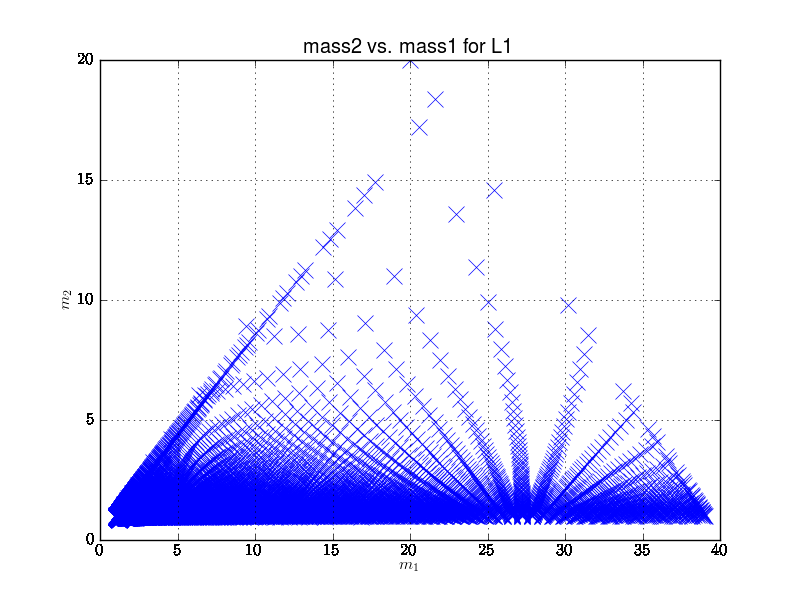
\includegraphics[scale=0.40]{Images/L1_m1m2_tmpltbank_GRB070429B.png}
%\caption{Template bank in $m_2$ vs. $m_1$ -- the $m_2$ is the mass of the larger component.}
%\label{templatebankL1}
\end{minipage}
\hspace{0.5cm}
\begin{minipage}[b]{0.5\linewidth}
%\centering
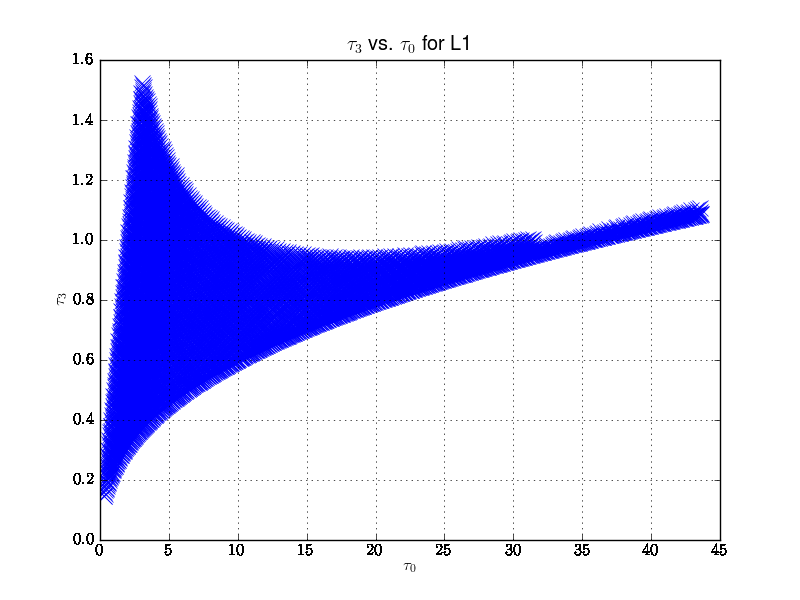
\includegraphics[scale=0.40]{Images/L1_tau0tau3_tmpltbank_GRB070429B.png}
\end{minipage}
\caption{Left figure: template bank in $m_2$ vs. $m_1$ -- the $m_2$ is the mass of the larger component. Right figure: template bank in $\tau_3$ vs. $\tau_0$. The templates are more evenly distributed in $\tau_0$ vs. $\tau_3$ space; this is because the parameter space is approximately flat in $\tau_0$ and $\tau_3$, as discussed .}
\label{tauL1}
%\end{minipage}
\end{figure}

Thus, by using an appropriate set of template waveforms, called a \emph{template bank} in mass space (more precisely in $\tau_0-\tau_3$ space), one can cover all masses in the desired mass interval with some predetermined maximum loss in SNR. Typically, searches will implement a template bank with a maximum SNR loss of 3$\%$, which leads to template banks containing of the order of a few hundred templates (the exact number depends on the detector's noise power spectrum).

\section{The $\chi^2$ test}
\label{chisq_theory}

When noise is Gaussian and stationary the matched filtering technique gives the best probability to find a signal with a before--known waveform. In non--Gaussian data, noise transients (``glitches'') that do \emph{not} match the template but still give high SNR are present. It is necessary to have some way of distinguishing the glitches from true signals.

The method which has become standard for this, is to use a \emph{chi--squared} (${\chi}^2$) veto test \cite{Allen:2004gu}. When a template exceeds a certain threshold SNR, it is then divided into $N$ different frequency bands such that each band should yield $1/N$ of the total SNR of the data if the high SNR event was a signal matching the template. The sum of the squares of the differences between the expected SNR and the actual SNR from each of the $N$ bands is then calculated (the ${\chi}^2$ statistic). The advantage of using the ${\chi}^2$ veto is that glitches tend to produce large ${\chi}^2$ values, and are therefore distinguishable from true gravitational waves signals. Thus, only those template matches with low enough ${\chi}^2$ values are kept for further analysis. We will further detail the theoretical framework of the $\chi^2$ test.

Following the analytic treatment of \cite{Harry:2011qh,ian}, suppose at a given time $t$ the signal in a GW detector will have three components: a Gaussian noise component $n(t)$, a GW signal component that matches a template $h(t)$ and a non--Gaussian component that would match a ``glitch'' template $g(t)$:
%
\begin{equation}
s(t) = n(t) + \alpha h(t) + \beta g(t)
\end{equation}
%
where $\alpha$ and $\beta$ are amplitude terms. $h(t)$ and $g(t)$ are orthogonal and normalized:
%
\begin{equation}
  ( g | g ) = 1 \, , (h | h) = 1 \, ,  ( g | h ) = 0 \, .
\end{equation}
%
In order to construct a $\chi^{2}$ test, we must introduce an additional set of $N$ template waveforms $T^{i}$ to the ones already existing in the template bank. These waveforms are required to be orthonormal and orthogonal to the template bank waveforms denoted by $h$,
%
\begin{equation}
\mathrm{orthogonal ~to}~h(t):  (h|T^i) = 0
\end{equation}
%
\begin{equation}
\mathrm{orthonormality:} ~(T^i | T^j) = \delta^{ij}
\end{equation}
%
The $\chi^{2}$ discriminator is constructed as a sum of squares of the match between $T^i$ and the data stream $s$:
%
\begin{equation}\label{eq:chi2}
  \chi^2 = \sum_{i=1}^{N} (T^i | s)^2 \, .
\end{equation}
%
When the data comprises only signal $h$ and and Gaussian noise $n$, the $\chi^2$ will be
%
\begin{equation}
  \chi^2 = \sum_{i=1}^{N} (T^i | n)^2
\end{equation}
%
and the statistic is the sum of squares of independent Gaussian variables with zero mean and unit variance. Thus the test is $\chi^{2}$ distributed with $N$ degrees of freedom, with a mean and variance of
%
\begin{equation}
  \langle\chi^2\rangle = N
  \quad
  {\rm Var}(\chi^2) = 2N
\end{equation}

In the case where the data is not an exact match to the signal, we take both $\alpha$ and $\beta$ to be non--zero, i.e., any signal or glitch can be linearly decomposed into a part $\alpha h(t)$ and a second orthogonal part $\beta g(t)$. In this case the $\chi^{2}$ test takes the form
%
\begin{equation}
  \chi^2 = \sum_{i=1}^N \left[ (T^i | n)^2 + 2 \beta (T^i | n)(T^i | g) +
  \beta^{2} (T^i|g)^2 \right] \, .  
\end{equation}
%
This has a mean
%
\begin{equation}
  \langle\chi^2\rangle = N + \beta^{2} \sum_i^N (T^i | g)^2
\end{equation}
%
and a variance
%
\begin{equation}
  {\rm Var}(\chi^2) = 2N + 4 \beta^{2} \sum_i^N(T^i|g)^{2} \, .
\end{equation}
%
The $\chi^{2}$ statistic is distributed as a non--central $\chi^{2}$ distribution with $N$ degrees of freedom and a non--centrality parameter \cite{Allen:2004gu}
%
\begin{equation}
  \lambda =  \beta^{2} \sum_{i=1}^N (T^i | g)^2
\end{equation}
%
Let
%
\begin{equation}
 \rho_{\mu}^i =
  \frac{(s | h_{\mu}^i)}{\sqrt{(h_{\mu} | h_{\mu})}}
\end{equation}
%
be the \ac{SNR} contribution in the $i$th frequency bin for the $\mu$th amplitude term. The $\chi^{2}$ statistic is then constructed as
%
\begin{equation}
  \chi^2 = N \sum_{i=1}^N \sum_{\mu = 1}^4 (\rho_{\mu}^i - \rho_{\mu}/N)^2.
\end{equation}
%
As all the components are orthogonal it is easy to see that this statistic will be exactly $\chi^{2}$ distributed with $4(N - 1)$ degrees of freedom. In a coherent way, one can interpret this as the sum of the single detector $\chi^{2}$ values for the $h_{0}$ and $h_{\frac{\pi}{2}}$ waveforms in the synthetic $+$ and $\cross$ detectors. This simply means that the ${\chi}^2$ threshold, ${\chi}^*$, depends quadratically on the measured SNR, ${\rho}$, as well as linearly on the mismatch $\Delta T$ (the threshold represents the maximum value of the $\chi^2$ assigned to signals; it is set fixed for an analysis). The main challenge to constructing a working $\chi^2$ test is the adequate choice of templates $T^i$ to model the effect of glitches in the \ac{GW} data streams \cite{Harry:2011qh,ian}. These are constructed by taking into account three factors: the accuracy of the waveform, the template bank mismatch up to a maximal loss in optimal SNR of 3\%; the uncertainties in instrumental calibration affecting the match between signal and template. Therefore, the coherent analysis will construct three different $\chi^2$ tests to account for these challenges -- we refer the reader to Chapter \ref{Chapter Four}, Section \ref{coh_search_grb}, for an overview of these tests.

\section{Horizon distance}
\label{horizon_distance_theory}

In assessing the overall performance of a detector for CBC searches, we use two representative numbers: the inspiral horizon distance to identify the ``typical'' sensitivity of the interferometers in terms of distance range (which is closely related to the PSD) and the live--time of the detector to identify the amount of time the detector has been on and taking science--mode data during a search (which is closely related to the amount and types of data quality vetoes that are applied to the data, see Chapter \ref{Chapter Four} for reference).  

The inspiral horizon distance of a detector is the distance at which an optimally--oriented and optimally--located equal--mass compact binary inspiral would give an average SNR of $\rho=8$ in the interferometer \cite{Abadie:2010cg}. We find the inspiral horizon distance by setting $\langle \rho \rangle = 8$ in equation (\ref{eq:cbc_fouriermagic}) and solving for the distance $D$ to the inspiral event which parameterizes the waveform $\tilde{h}(f)$.  Thus, the inspiral horizon distance combines the spectral density curve (PSD) with the expected inspiral waveform to produce a single quantity that summarizes the sensitivity of the detector at a given time.

Due to the fact that the detector operates over a frequency range which is not bound at infinity, modifications to the limits of the integral need to be applied.  In the CBC search, we compute the signal to noise ratio by
\begin{eqnarray}
\label{range} \langle \rho \rangle= \sqrt{4 \int_{f_{low}}^{f_{high}} \frac{|\tilde{h}(f)|^2}{S_n(f)} df}.
\end{eqnarray}
The lower limit is determined by the detector's behavior at low frequencies.  In the S5 CBC search the lower frequency cut--off limit was set to $f_{low}=40$ Hz in computing the inspiral horizon distance, since this corresponds to the seismic threshold frequency \cite{Macleod:2011up}.  For Virgo in VSR1, the low frequency cut--off was higher at $f_{low}=60$Hz.  The upper integration bound is the innermost stable circular orbit (ISCO) frequency that separates the inspiral phase to the merger phase (see Chapter \ref{Chapter One} where we have already introduced ISCO)

\begin{eqnarray}
f_{isco} = \frac{c^3}{6\sqrt{6}\pi G M},
\end{eqnarray}
%
where $M$ is the total mass of the binary system.  For binary neutron star systems, $f_{isco}= 1570$Hz.  However, during S5/VSR1 the sampling frequency of the 2048s. blocks used to compute the PSD was $f_{\mathrm{Nyquist}}$ = 2048 Hz. This difference in the upper limit of the frequency has a negligible effect due to the fact that most of the power in SNR is accumulated in the high--sensitivity ``bucket'' of the PSD (see Chapter \ref{Chapter One}, Figure \ref{ligonoise} -- the ``bucket'' is in the region of 100 Hz for LIGO).

For an optimally--oriented and optimally--located equal mass binary, the signal that appears at the interferometer in the approximation of the stationary phase waveform is given by (see Chapter \ref{Chapter One}, equation (\ref{eq:cbc_hp_hc_spa})):

\begin{eqnarray}
\label{spa}
\tilde{h}(f) =  \frac{1}{D}\left(\frac{5\pi }{24c^3}\right)^{1/2}(G\mathcal{M})^{5/6}(\pi f)^{-7/6} e^{i\Psi(f;M)},
\end{eqnarray}

\noindent where $\mathcal{M}$ is the chirp mass of the binary, $D$ is the distance to the binary and $\Psi$ is a real function of $f$, parameterized by the total mass $M$.  Setting $\langle \rho \rangle = 8$ and inserting this waveform into equation (\ref{range}), we find that the inspiral horizon distance is given by:

\begin{eqnarray}
\label{range0} D = \frac{1}{8}\left(\frac{5\pi }{24c^3}\right)^{1/2}(G\mathcal{M})^{5/6}\pi^{-7/6} \sqrt{4 \int_{f_{low}}^{f_{high}} \frac{f^{-7/3}}{S_n(f)}df },
\end{eqnarray}

\noindent where $D$ is expressed in Mpc. The horizon distance is usually calculated for equal mass components. The mean inspiral horizon distance as a function of component mass for the four gravitational wave detectors H1, L1, H2 and V1 during all of S5 and VSR1 science runs is shown in Figure \ref{rangevmass}.

\begin{figure}[ht!]
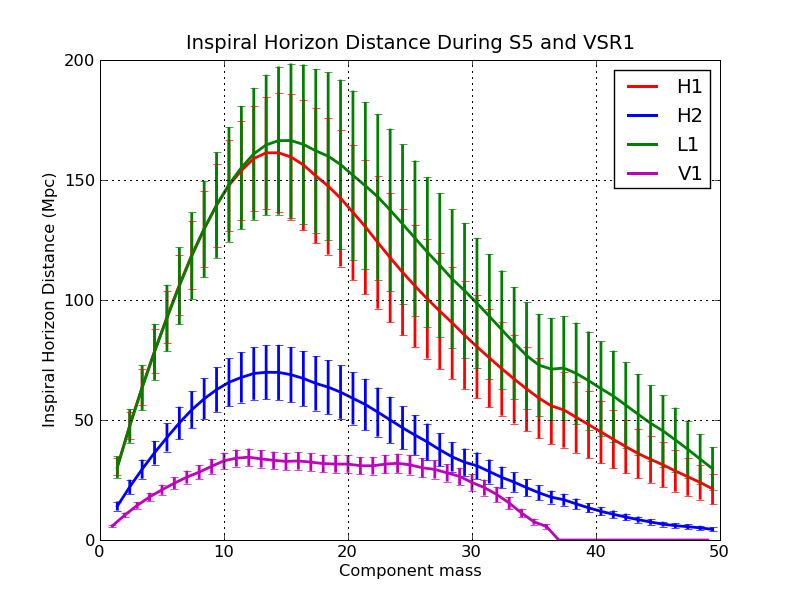
\includegraphics[scale=0.65]{Images/horizon_distance_S5.png}
\caption{Mean inspiral horizon distance as a function of component mass for the four gravitational wave detectors H1, L1, H2 and V1 during all of S5 and VSR1 science runs.  The error bars attached to the points indicate the standard deviation in the inspiral horizon over the course of each of the weeks of the science runs; the error bars extend from one standard deviation below to one standard deviation above the mean. Image first published and reproduced from \cite{Abadie:2010cg}}
\label{rangevmass}
\end{figure}

\newpage
In this chapter we have introduced a series of key theoretical concepts that are used in gravitational waves data analysis. In the next chapter, Chapter \ref{Chapter Four}, we will present the practical use of these concepts in the analysis process with direct application to GW data analysis associated with short GRB triggers.


\chapter{Gravitational waves: coincident and coherent searches with short GRB triggers} % Write in your own chapter title
\label{Chapter Four}

\section{Introduction}
In Chapter \ref{Chapter Two} we have outlined the importance of searches for GW triggered by short GRBs whereas in Chapter \ref{Chapter Three} we have described a theoretical background of the analysis techniques used to search for CBC events, in general. These methods have been implemented in two different search \emph{``pipelines''} (coincident and coherent) that have been built for the specific role of searching for CBC events in association with short hard GRBs. ``Pipeline'' refers here to the ensemble of data processing stages that are built to implement the theoretical concepts described in Chapter \ref{Chapter Three}; a pipeline takes the GW detectors' data as input and outputs a list of possible detection events; based on the significance of these events, either a GW detection statement is made, or exclusion distances are computed. 

I used and contributed to the development of both the coincident and coherent pipelines and I will present the workflow, the usage and the search results of these pipelines by means of two examples: a search for CBC events associated with GRB070429B -- in the case of the coincident search during S5/VSR1 and GRB090831A -- in the case of the coherent search during S6/VSR2 and 3. To place these example searches into context, I will also briefly present the search results for GW associated with short GRBs both during S5/VSR1 and S6/VSR2 and 3 science runs.

\section{Coincident triggered search}
\label{coincident_GRB}

Searches for GW associated with short hard gamma-ray bursts have been completed over the last two LIGO and Virgo science runs, see Table \ref{tab:sciencetimes} for the exact dates of these runs, consult \cite{Abadie:2010uf} for results in S5/VSR1 and \cite{lvc:s6grb} for results in S6/VSR23. During S5/VSR1, 22 short hard GRBs observed by \emph{Swift} have been analyzed whereas during S6/VSR2 and 3, 16 GRBs observed by \emph{Swift} and an additional 10 observed by Fermi--GBM have been analyzed. The S5/VSR1 GRBs have been analyzed using the coincident pipeline, described in this section with the help of an example GRB. The S6/VSR2 and 3 GRBs have been analyzed using the coherent pipeline described in the next section, again with the help of an example GRB.

\begin{table}[tp!]
\center
%\begin{ruledtabular}
\begin{tabular}{c | c | c}
\hline
\hline
Science run & Start time & End time \\
\hline
\hline
LIGO -- S5 & 4 November 2005 & 30 September 2007 \\
\hline
Virgo -- VSR1 & 18 May 2007 & 30 September 2007 \\
\hline
LIGO -- S6 & July 7 2009 & October 20 2010 \\
\hline
Virgo -- VSR2 & July 7 2009 & January 11 2010 \\
\hline
Virgo -- VSR3 & August 11 2010 & October 20 2010 \\
\hline
\hline
\end{tabular}
%\end{ruledtabular}
\caption[Duration of LIGO and Virgo science times.]
{The dates of LIGO and Virgo science run times for S5/VSR1 and S6/VSR2 and 3.}
\label{tab:sciencetimes}
\end{table}

Both the coincident and coherent triggered searches use the time and the sky position of the GRB (provided through astronomical observations using the GRB missions and publicly available in NASA's Gamma-ray Circular Notes or GCN, see \cite{gcns}) and uses this information to limit the search to a small time interval and a narrow positional sky error region. The search utilizes the ``coincidence'' technique in which data from all of the detectors is analyzed separately, before looking for events which are coincident between detectors. The coincident triggered search implementation described here is used to search for \ac{CBC} systems whose total masses lie between 2 and 35 $M_{\odot}$ with a minimum component mass of 1 $M_{\odot}$. This choice is motivated by the accepted theory that short GRBs originate from either NS--NS or NS--BH binary coalescences with typical NS masses of 1.4 $M_{\odot}$ and BH masses of 10 $M_{\odot}$ \cite{Abadie:2010uf}. During both S5/VSR1 and S6/VSR2 and 3 an ``ihope'' all--sky--all--time search was carried out as well. The infrastructure the triggered search uses is very similar to the ``ihope'' search described in \cite{Abbott:2009qj} with the exception that the search is done on a much reduced area of the sky and uses a much smaller analysis time around the GRB, thus increasing the sensitivity (see Section \ref{sens_imprv} for a sensitivity comparison between the all--sky, all--time search using ``ihope'' and the GRB triggered search).

The main analysis steps (pipeline workflow) are as follows: data around the time of a short GRB is divided into one ``foreground'' region (containing the GRB event time and where we expect the GW signal to be found) and two ``background'' regions on either side of the ``foreground'' (where we expect no GW signal associated with the GRB). Data from individual operational GW detectors is matched--filtered through detector--specific template banks and using detector--specific PSDs -- the result will be a time--ordered list of events for each detector. Next, the pipeline looks for coincident events within this list (in time and recovered template masses) from all the detectors and applies the $\chi^2$ test on the new coincidences to filter out ``glitches''. The surviving events are collected and a ``detection statistic'' is computed for each, using the match--filter SNR and $\chi^2$ values. Simulated signals are injected in the ``background'' data stretch to test and compute the pipeline's efficiency of signal recovering. Using this efficiency and the ``detection statistic'' of the loudest events, we compute a probability that the loudest ``foreground'' event does or does not belong to the ``background'' statistical sample. In other words, if the event is a signal or noise. In the next sections, we will detail each of these analysis steps and provide the appropriate search results.

\subsection{GRB070429B -- overview}
\label{grb070429boverview}

GRB070429B (GRBlog entry \cite{070429b}) was a short hard gamma-ray burst that was observed on April 29, 2007 at 03:09:04 UTC by the \emph{Swift}/XRT/UVOT satellite. Its characteristic $T_{90}$ duration was 0.5 s and its sky location was right ascension RA=328.02 $\deg$ and declination dec=-38.84 $\deg$. The GRB has a secure host association from a faint sub--arcsecond (position within the UVOT error circle) of an optical afterglow and the host galaxy appears to be a red galaxy \cite{Cenko:2008vt} at redshift $z$=0.904 (luminosity distance of $\approx$4 Gpc). Although this burst has an associated redshift with a corresponding luminosity distance much larger than the typical GW detector range during S5/VSR1 (see Chapter \ref{Chapter Three}), we still performed a GW search since there is a degree of uncertainty in measuring short burst redshifts (see Chapter \ref{Chapter Two} for a reference on assigning redshifts and luminosity distances to short GRB). 

LIGO's operational detectors at the time of the burst were Hanford H1 and Livingston L1. The antenna factors $F = \sqrt{F_{\times}^2+F_+^2}$ for H1 and L1 are 0.99 and 0.93 respectively giving an overall antenna factor of 0.96, revealing an almost overhead position with respect to the H1L1 plane. The astronomical and GW detector data summarizing the characteristics of GRB070429B is presented in Table \ref{Table_grb070429b}.

\begin{table}[ht]
 \begin{tabular}{|l|l|l|l|l|l|}
 \hline
 \hline
 GPS & Date & redshift & $T_{90}$ (s) & RA ($\deg$) & dec($\deg$) \\
 \hline
 861851358 & Apr 29, 2007, 03:09:04 UTC & 0.904 & 0.5 & 328.02 & -38.84 \\
 \hline
 \hline
 \end{tabular}
 \caption{Astronomical and GW detector data for GRB070429B. GRB070429B is a very short gamma-ray burst with $T_{90}$ duration of only 0.5s. The GRB was observed almost overhead by the GW detectors (H1 and L1, with an RMS antenna factor of 0.96). The confirmed redshift of the burst places it at a distance of $\approx$4 Gpc.}
 \label{Table_grb070429b}
\end{table}

\subsection{Data Segments and PSD generation}
\label{grb070429bsegments}

The binary coalescence model of short GRB formation predicts that the time delay between the arrival of a gravitational wave and the arrival of the subsequent gamma-ray burst is a few seconds, see Chapter \ref{Chapter Two}, section ~\ref{SHBmodel}. The gamma-ray burst arrival time is called the \emph{GRB trigger time} and, in this case, it is provided by the \emph{Swift} satellite. We search for gravitational wave signals within an \emph{``on--source''} segment of [-5, +1) s. around the GRB trigger time; this time window should theoretically account for all the the SHB model--dependent uncertainties as well as for the gamma-ray detector's instrumental timing uncertainties.

Since we rely on the assumption that a gravitational wave associated with a GRB should only be detected in the on--source segment, we use off--source \emph{trials} (324, each trial with the length of the on--source, 6 s long) that do not intersect the on--source, to estimate the distribution of \emph{background} due to the accidental coincidences of noise events. We also re--analyze the off--source trials with simulated signals injected in the data to test the response of the search to GW signals; these we call injection trials. To prevent accidental bias in the background estimation due to a potential loud and prolonged signal in the on--source, the off--source segments are padded with 48 s long redundant \emph{buffer} segments on each side of the on--source, the length of these reflecting the longest duration of a matched--filtering waveform. Finally, we discard 72 s of data subject to filter transients on both ends of the off--source region. Taking all these requirements into consideration, the minimum analyzable time \emph{required} for the GW data stretch was $T_{\mathrm{analysis}}=$2190 s and we require that GW detectors should be in continuous science mode for this time, as the character of the background can change between science mode stretches. The data segments are shown in Figure ~\ref{grbsegments}. As we can see the GW detectors with available segments to meet these criteria are H1, H2, G1 and L1. For the S5/VSR1 coincident GRB analysis, the two most sensitive detectors per GRB analysis were used to provide the data; in the case of GRB070429B the two most sensitive detectors were Hanford H1 and Livingston L1.

Both the H1 and L1 strain data were sampled at 16384 Hz. This frequency is actually too high since the highest frequency in each of the matched--filter waveforms is $\approx$2 kHz. To ease computational requirements, the time series is down-sampled to 4096 Hz prior to analysis and a low--pass filter is applied with a cut--off frequency at 2048 Hz. At the lower end of the frequency spectrum, the data is affected by seismic noise (see Chapter \ref{Chapter One}) and a series of high--pass filters are applied to limit the low--frequency at 40 Hz. The power spectral density (PSD) is calculated independently on every 2048s block of data. These blocks are divided in 15 blocks of 256 s each. The PSD for each of these 15 overlapping blocks is constructed by taking the median in each frequency bin. 

\begin{figure}[ht]
\centering
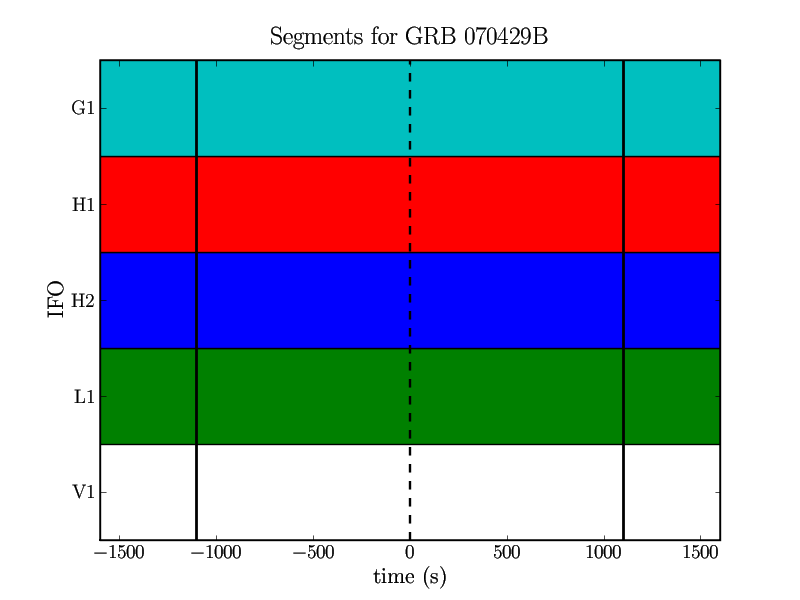
\includegraphics[scale=0.30]{Images/GRB070429B_segments.png}
\caption{Data segments availability for GRB070429B -- the "0" line represents the trigger time (the burst arrival time recorded by \emph{Swift} satellite); solid colors for the IFO (detectors) show continuous science--mode.}
\label{grbsegments}
\end{figure}

\subsection{Two--stage coincident pipeline}
\label{pipeline}
\paragraph{Pipeline overview}

Data streams from each detector participating in the search are first analyzed separately. As this is a coincidence search, the first stage of the pipeline is to determine if there is any loud \ac{SNR} event in any of the detectors. For each detector the process is to:
%
\begin{itemize}
 \item Generate a template bank to cover the full mass range.
 \item Filter the data against every template in the bank for each detector.
 \item Retain a ``trigger'' whenever a loud \ac{SNR}, above a certain threshold, is observed.
\end{itemize}
%
This results in a list of single detector triggers for each detector. The lists are then examined for any triggers that are coincident between detectors. A trigger is discarded if it is not seen in more than one detector. Coincidence is determined using the masses of the templates as well as the observed time.

In reality, the GW detector data is neither stationary nor Gaussian and to minimize these effects a two--stage coincident pipeline is used, with a schematic in Figures \ref{cbcstage1} and \ref{cbcstage2} for the analysis of GRB070429B that used data from H1 and L1 detectors. Each of the stages will be described in detail in the next subsections and here we provide just a brief overview: the first stage of the pipeline takes the calibrated $h(t)$ from H1 and L1 (calibration is not covered in this work but references can be found here in ~\cite{Abadie:2010px, Allen:1996, Adhikari:2003}) and constructs a template bank populated with theoretical waveforms through which the calibrated data will be matched--filtered. The resulting matched--filtering events will be tested for coincidence status in both H1 and L1, and if coincidences are found, these events will form the basis of the second stage of the pipeline. The coincident events will have their templates reconstructed collectively into a new template bank through which the resulting stage one triggers will be match--filtered. Signal--consistency veto tests will be applied at this level and the surviving triggers will be tested again for coincidence. The final steps of the second stage involve constructing a combined statistic of the coincident events (together with the results of the signal--consistency tests) and a final ranking of the events according to this statistic, leading to false alarm estimation and a detection statement.
%
\begin{figure}[htb!]
\centering
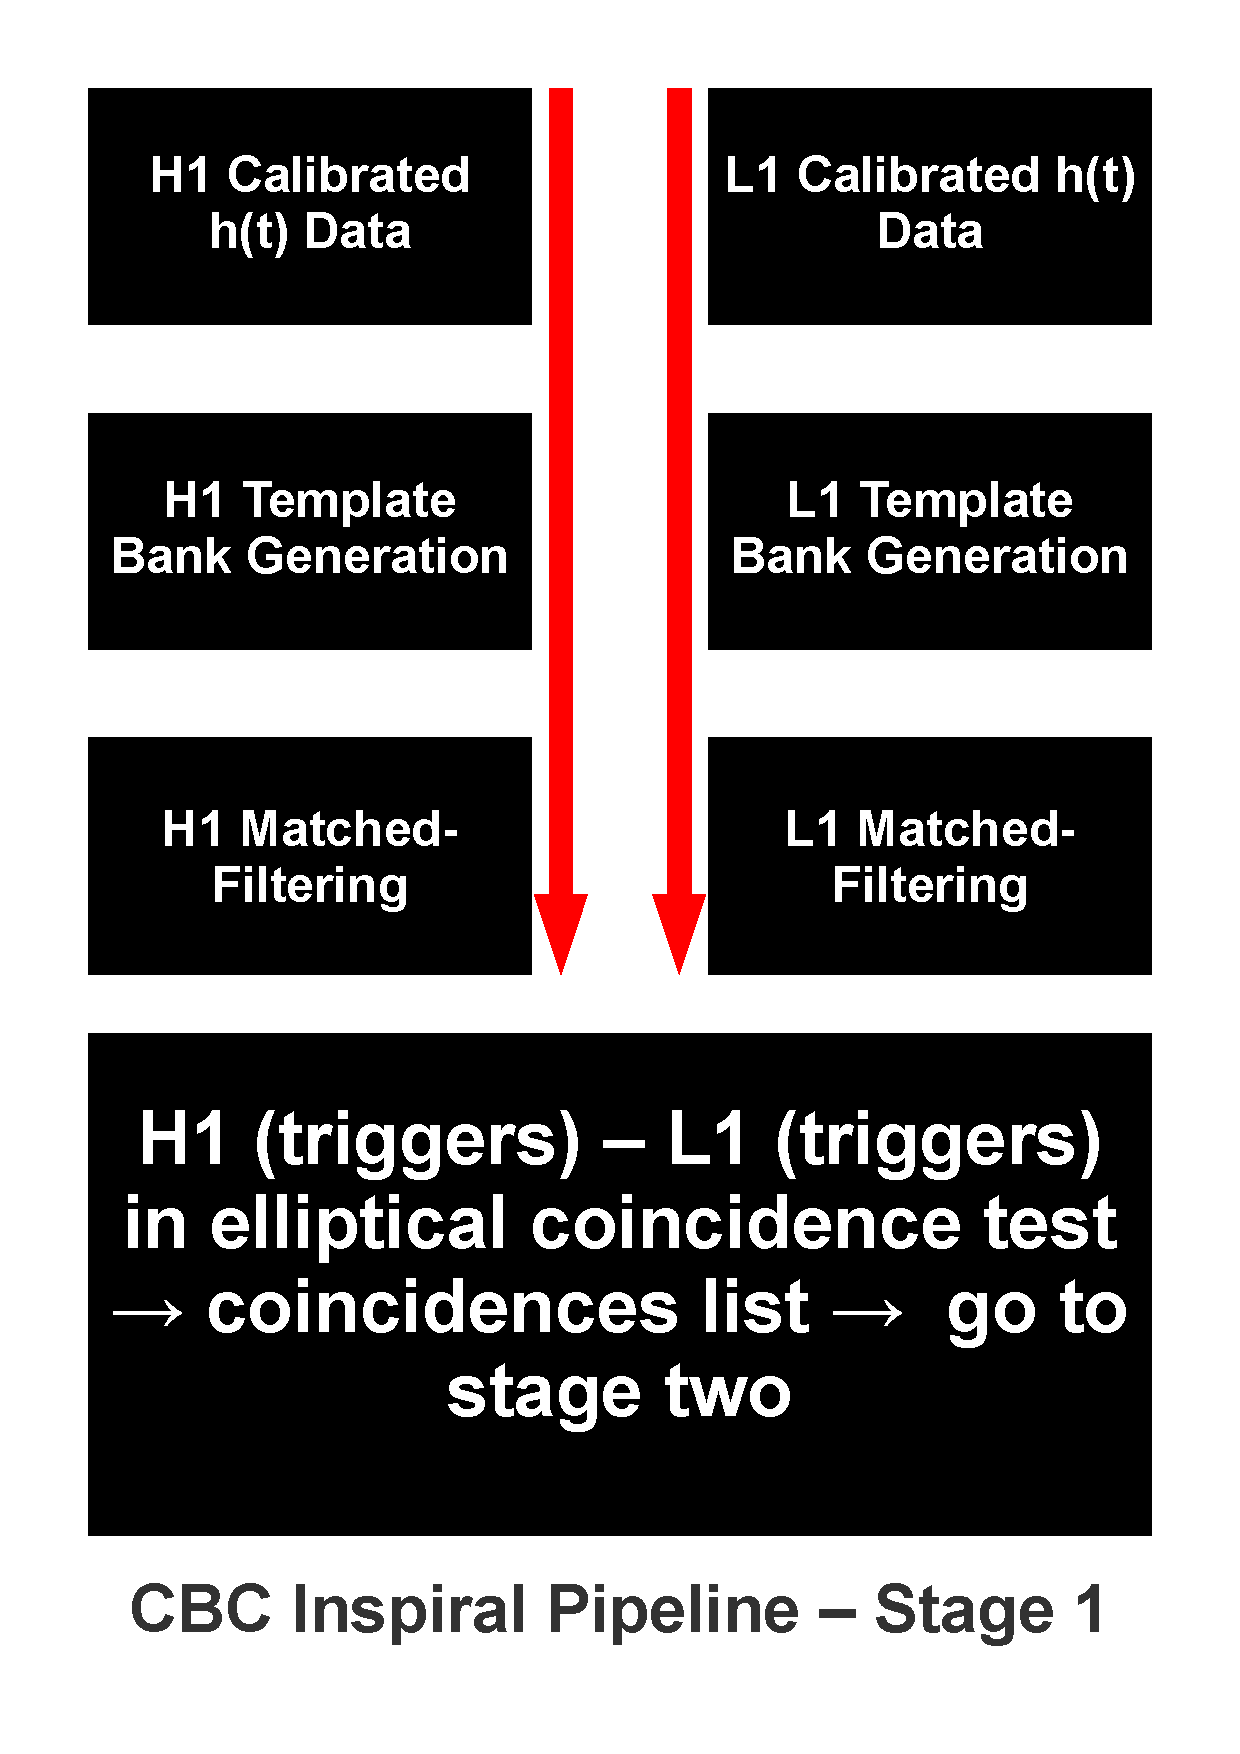
\includegraphics[scale=0.4]{Images/CBC_Stage_1.pdf}
\caption{Stage 1 of the CBC inspiral pipeline}
\label{cbcstage1}
\end{figure}
\begin{figure}[htb!]
\centering
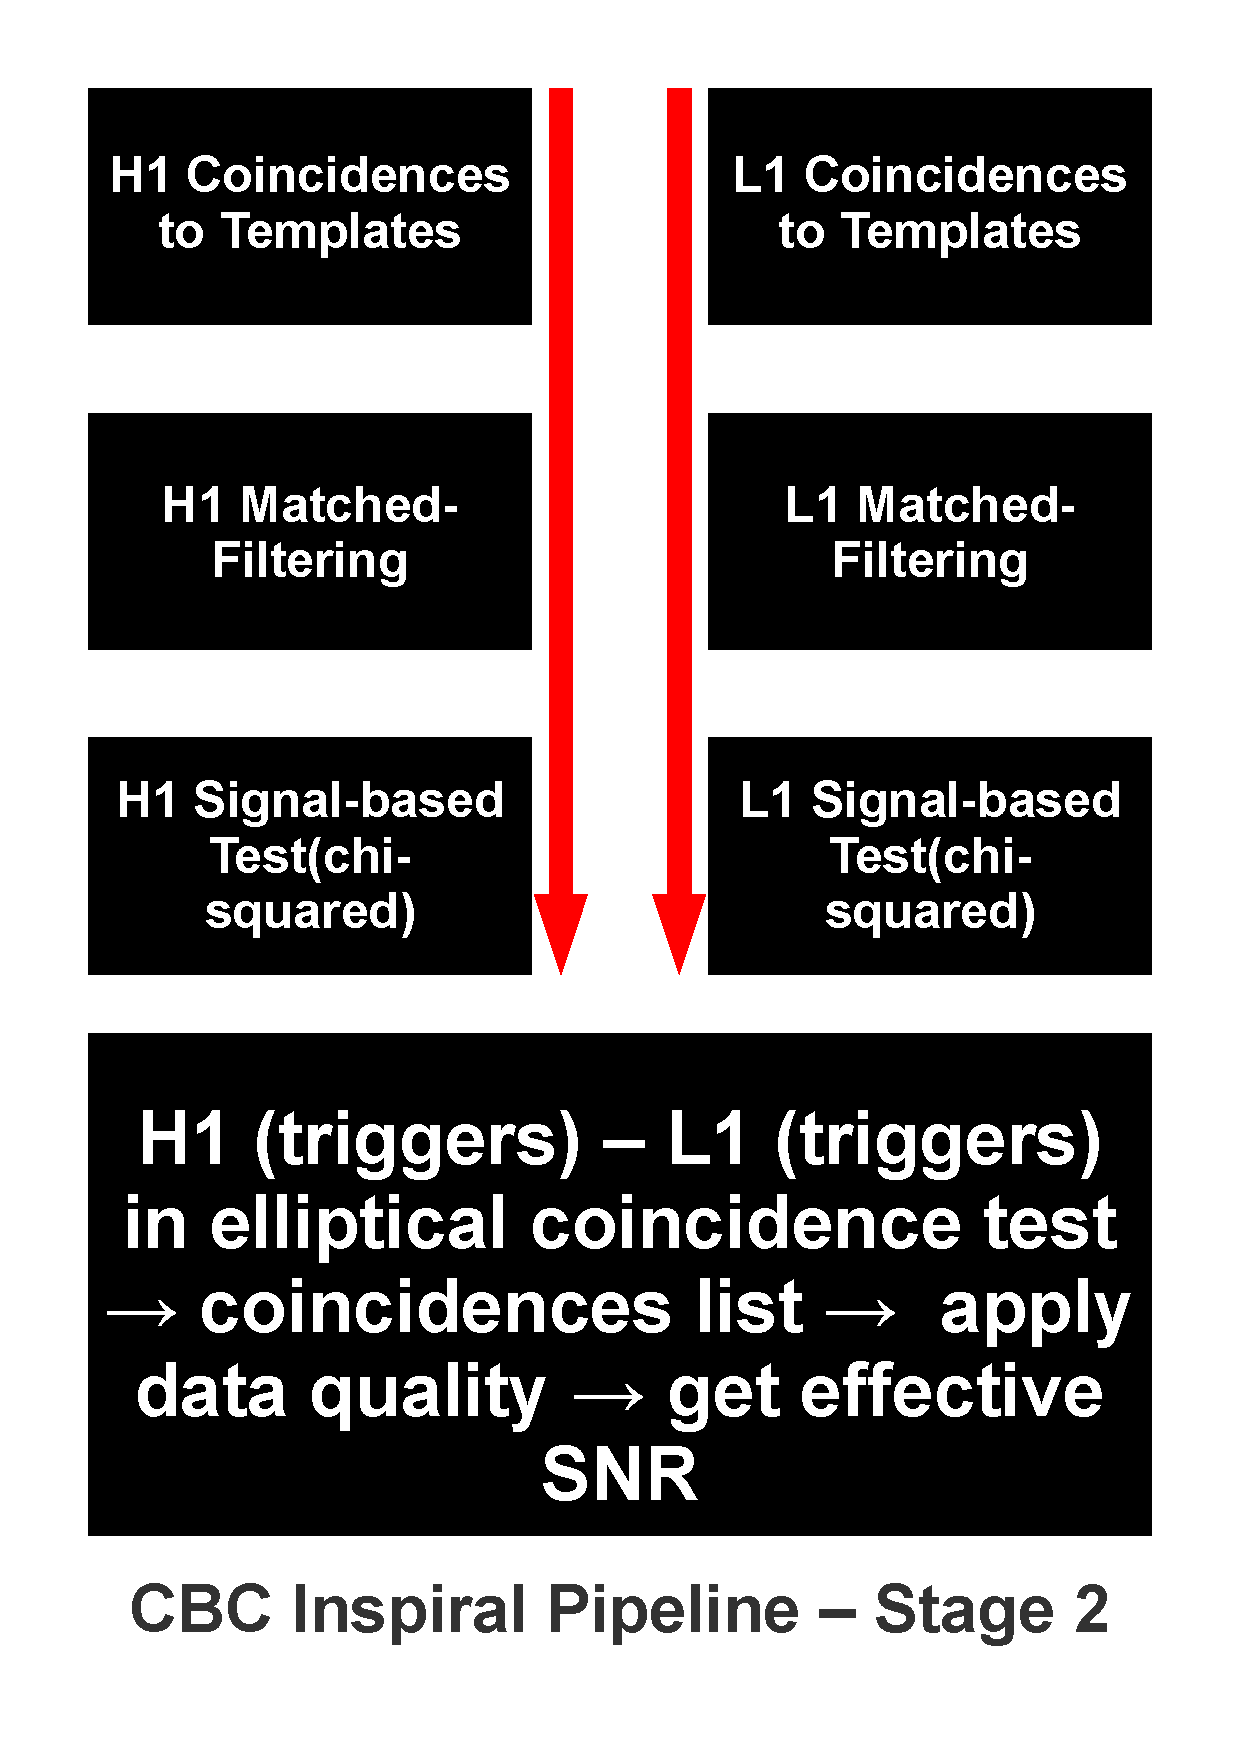
\includegraphics[scale=0.4]{Images/CBC_Stage_2.pdf}
\caption{Stage 2 of the CBC inspiral pipeline}
\label{cbcstage2}
\end{figure}
%

\subsection{Template bank}

In the case of GRB070429B, the matched--filtering was done using a non--spinning waveform template bank that was symmetric in component masses in the interval ~$2 \times M_{\odot} \leq M < 40 \times M_{\odot}$ in total mass $M$ \cite{Abadie:2010uf}. The number of template waveforms depends on the sensitivity of the detector and in this case, having to analyze data from H1 and L1, $\sim$~6000 templates have been used for H1 and $\sim$~9000 for L1 respectively, due to its flatter noise curve. For the GRB070429B search $\tilde{h}_0$ is calculated directly in the frequency domain using the ``TaylorF2'' Post--Newtonian approximate waveforms as described in \cite{Blanchet:2001dw} (see Chapter \ref{Chapter One} for a short explanation of Post--Newtonian formalism).

\subsection{Trigger generation}
Equation (\ref{eq:cbc_lowsnr}) gives the maximized SNR that can be calculated at all times in the segment being analyzed using equation (\ref{eq:cbc_fouriermagic}). The result of matched--filtering through the template bank is a discrete time--series of \emph{triggers} with various SNRs as measure of their ``loudness''. As an illustration, the time--series of triggers from H1 is plotted in Figure \ref{H1snr} for GRB070429B. It is easy to show that the expected distribution of $\rho^2$ in Gaussian noise will follow a $\chi^2$ distribution with two degrees of freedom. Triggers are retained only where the SNR at that point in time is larger than a threshold SNR $\rho_0$ and is the largest SNR within a small time interval. The number of triggers significantly increases below this threshold value of the SNR. The SNR threshold for the matched filtering step was chosen differently depending on which detectors are available for a given GW--GRB search. If data from H1 and L1 were analyzed, the threshold for each detector was set to $\rho_0 = 4.25$, reflecting their comparable sensitivity. If data from H1 and H2 were analyzed, the threshold of the latter detector, the less sensitive of the two, was set to 3.5 to gain maximum network sensitivity, while the threshold of the more sensitive detector, H1, was set to $\rho_0 = 5.5$ since any signal seen in H2 would be twice as loud in H1, with some uncertainty. For triggers with SNR $\rho > \rho_0$, the template masses and the time of the maximum SNR are recorded. For a given template, threshold crossings are clustered in time domain using a sliding window equal to the duration of the template \cite{Allen:2004gu}. For each trigger identified in this way, the coalescence phase and the effective distance -- the distance at which an optimally oriented and optimally located binary, with masses corresponding to those of the template, would give the observed SNR are also computed.

\begin{figure}[ht!]
\centering
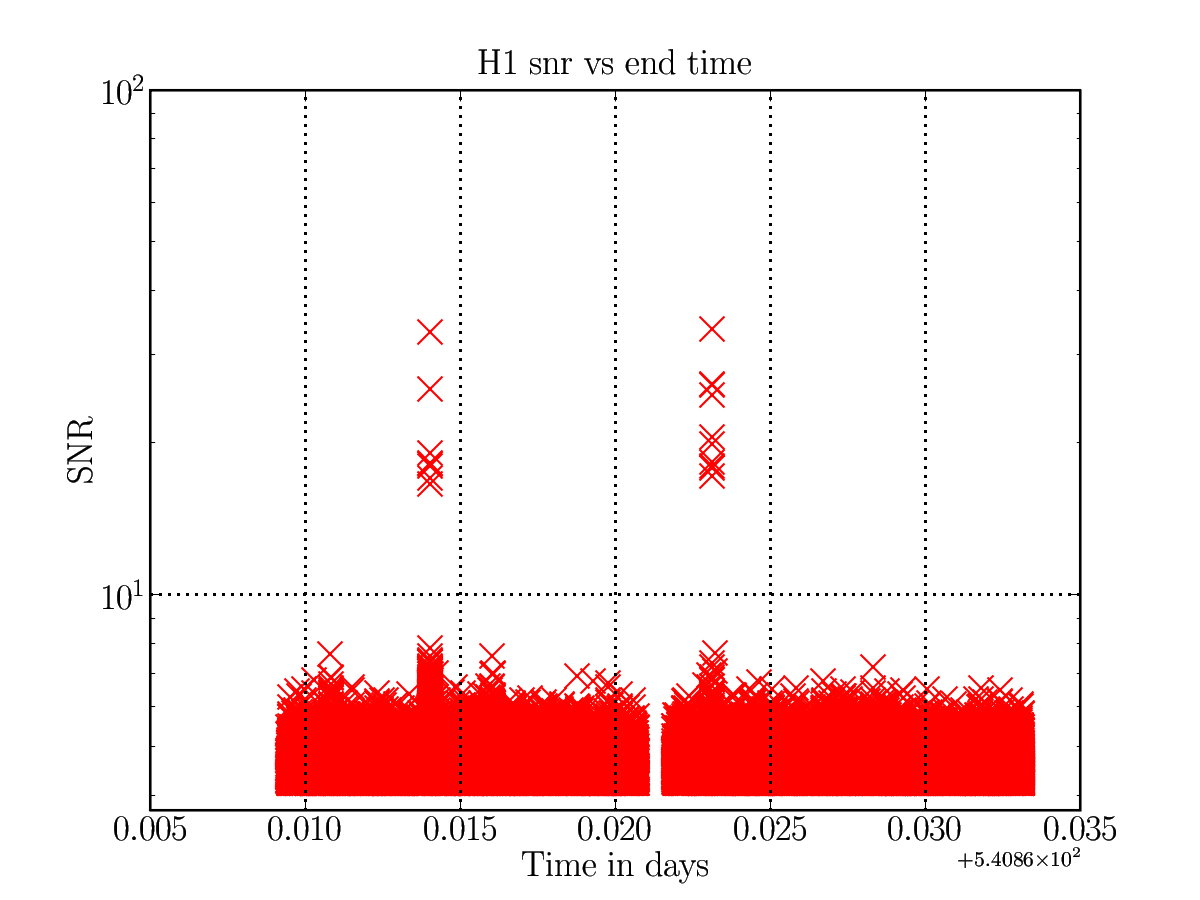
\includegraphics[scale=0.30]{Images/H1_SNR_time.png}
\caption{SNR time--series for Hanford H1 triggers for GRB070429B. We notice two loud glitches with SNR$\approx$40; the gap region corresponds to the ``on--source'' segment that we will examine visually only at the end of the analysis.}
\label{H1snr}
\end{figure}

Each non--Gaussian noise event has the tendency to match a series of different templates, usually high chirp mass ones, creating clusters of triggers. Usually these triggers tend to have high SNR values and in an SNR time--series given in Figure \ref{H1snr} show up as loud events much above the background at lower SNRs.

\subsection{Coincidence test and coincidence events}
\label{grb070429bcoincidence}
In GW coincidence analysis, data sets from each detector will be analyzed separately, following the steps outlined above, and the resulting output of the matched filtering stage will be single--detector triggers with different masses and coalescence times. Since the effect of a GW should be the same at all the operational detectors, the analysis requires that triggers from each detector be \emph{coincident} -- the next step of the pipeline is to perform coincidence tests between the triggers that are produced in each of the detectors. Triggers are considered coincident if they occurred at the same time and have similar masses. The definition of trigger ``coincidence'', as used in the actual analysis, is given in \cite{Robinson:2008un}: the presence of noise causes errors in the measurement of parameters of an inherent signal; due to this, it is very improbable that the same gravitational wave in different detectors can be associated with \emph{exactly} the same set of masses and times. However, it should be possible to detect signals in coincidence by demanding that the measured parameters lie in a sufficiently small parameter window, called \emph{coincidence window} \cite{Robinson:2008un}.

Considering a three--dimensional trigger parameter space with coordinates identical to the template bank coordinates $\vec{\theta} = (t_c, \tau_0(m_1,m_2), \tau_3(m_1,m_2))$, the parametric distance between two signals (expected broadening due to noise) will be given by:

\begin{equation}
\mathrm{d}l^2 = g_{12}(\vec{\theta})\mathrm{d} \theta_1\mathrm{d}\theta_2 \sim \frac{1}{\rho^2}
\end{equation}

\noindent where the metric $g_{12}(\vec{\theta})$ is the same template bank metric and is defined on the $\vec{\theta}$ vector space given by equation (\ref{ethincametric}). Since in the presented analysis we used data from two detectors with two different PSDs, and the metric depends on the PSD, there will be two different metrics to choose from. This is resolved by generating an ellipsoid in the $\vec{\theta} = (t_c, \tau_0(m_1,m_2), \tau_3(m_1,m_2))$ space around every trigger, observed in each of the operational detectors, using the appropriate metric given the noise PSD of the detector. The ellipsoid size can be tuned before the analysis, so that for any given threshold, all the points within the distance $\mathrm{d}l$ lie within the ellipsoid. Since only triggers with similar time of coalescence $t_c$ can be coincident, it is useful to first sort the triggers by $t_c$ and then check for coincidences; this greatly reduces the computational costs. For every pair of independent detector triggers, the overlap of their corresponding ellipsoids is measured; the triggers are considered coincident if the distance $\mathrm{d}l$ is smaller than a certain threshold (ellipsoid thinca or e-thinca parameter). The smaller the e-thinca parameter is, the closer the two triggers are in the $\vec{\theta}$ parameter space, hence the better a coincidence is confirmed. The threshold is empirically set at 0.8 by investigating the distribution for triggers associated with simulated signals; this value corresponds approximately to the limit where the majority of simulations are not recovered. The triggers that survive the coincidence test are stored and component masses, coalescence phases and effective distances are computed from the templates they were matched against.

The $\chi^2$ signal consistency test, which we describe in detail in Chapter \ref{Chapter Three}, tests whether a potential trigger has the expected power in a number of different frequency bins (16 bins, in the GW--GRB search). The $\chi^2$ test is a very effective method of separating non--stationary noise events from true GW signals; unfortunately is is also very computationally intensive: a matched--filter needs to be calculated for every frequency bin. Therefore, the test is performed only when necessary: single detector $\chi^2$ is computed for every coincident trigger only at the second stage of the pipeline. 


The SNR--cut, coincidence and signal--consistency tests provide strong veto capacity to remove accidental noise triggers in the detector data that can not be coincident GW signals. The first stage matched--filtering of the data produced roughly 158$\times 10^3$ triggers for H1 and 210$\times 10^3$ triggers for L1 in the case of GRB070429B. After the first stage of the pipeline, where a cut on threshold SNR and the Ethinca test were applied, the total number of triggers was reduced to roughly 82$\times 10^3$ for H1 and 110$\times 10^3$ for L1 respectively, this accounting for a reduction of $\sim$50$\%$ in the total number of triggers. Further on, after the second stage of the pipeline, where matched--filtering was repeated and both coincidence and the $\chi^2$ tests were applied, the remaining number of coincidences was left to 4593. 

\subsection{Ranking statistic}
The SNRs and  $\chi^2$ test results from each detector are combined into an effective SNR that weighs less those triggers with large values of $\chi^2$ that are not likely to be GW signals. For a signal with relatively small SNR and an average value of the $\chi^2$ veto, the value of effective SNR is equal to the SNR. However, for a noise trigger with a large $\chi^2$ value, the effective $\rho$ is reduced according to equation (\ref{eqn:roeff}):

\begin{equation}
\rho^2_{\mathrm{eff}} = \frac{\rho^2}{\sqrt {( \frac {\chi^2}{2p-2})(1+ \frac {\rho^2}{250})}}
\label{eqn:roeff}
\end{equation}

\noindent In equation (\ref{eqn:roeff}), $p$ is the number of degrees of freedom in the $\chi^2$ measure, 16 for the coincident search. The denominator 250 is chosen to best separate the background (off--source) from signal. The effective SNRs from the analysis detectors are added in quadrature to obtain a cumulative effective SNR \cite{Abbott:2009tt,Abadie:2010yb}, in the case of GRB070429B we have H1 and L1 participating:

\begin{equation}
\rho^2_{\mathrm{eff}} = \rho^2_{\mathrm{effective, H1}} + \rho^2_{\mathrm{effective, L1}}
\end{equation}

\subsection{Data quality vetoes}
To reduce the number of triggers present due to non--Gaussian and non--stationary noise, it is useful
to try to identify times during which noise transients are likely to occur. These glitches are usually produced because of environmental causes to the detectors; these influence the detectors' optimal operation, e.g., increased seismic activity that produces low--frequency vibrations or electromagnetic disturbances that may produce glitches in high--frequency bands. For these reasons the detectors are continually monitored by a series of sensors, which survey the internal and external conditions. Work is constantly done on both monitoring the existent channels thought to produce noise glitches and trying to identify new noise channels. This effort is called \emph{detector characterization}. This information is used to flag the excessive noise periods and to discard the data that is associated with these times, process called \emph{vetoing}. For more details of these activities see \cite{Blackburn:2008ah,Macleod:2011up}.

To consider this from the point of view of the data analyst, it is sufficient to know whether
the data should be analyzed or not. The end product of the detector characterization process
is to assign all data a data quality category. Analyses for CBC signals treat these
data quality categories in the following way\footnote{
Note that there is also a category 4, but for CBC searches this category is only used when following up interesting triggers. Category 4 was not used on GRB070429B data.}
%
\begin{itemize}
 \item Category 1 veto: Data marked as category 1 indicates that the GW detectors don't operate in a correct way. This data is not used for any analysis and is not used to compute the noise PSD; it is discarded. As an example would be when the calibration cannot be attained and the strain $h(t)$ is not available; 
 \item Category 2 veto: Data marked as category 2 indicates that the detectors were operating normally but a mechanism \emph{known} to induce glitches in the data was active. This type of data \emph{may} be used to compute the noise PSD, however any trigger occurring during this time will be discarded.
 \item Category 3: Data marked as category 3 indicates that \emph{some} mechanism known to have some correlation with noise transients was active at the time this data was taken. Category 3 data \textit{is} analyzed and false alarm rates are calculated for coincident triggers occurring during category 3 data. Category 3 data is, however, discarded when calculating upper limits. An example
of a category 3 flag might be that there is elevated seismic noise at the time the data is
taken.
\end{itemize}

\subsection{Background estimation}

In order to make a GW detection statement, in the triggered GRB searches, we need to make a statement about the events that are obtained purely from detector noise, the \emph{background} where we don't expect any GW signals. Unlike the un--triggered searches that use non--physical times for background segments obtained from time--shifting data stretches, the triggered GRB searches use as background segments on either side of the on--source (a timesliding method has now been implemented in the triggered search as well, see Chapter \ref{Chapter Five}). Since the length of these segments is usually of $\approx1000$~s the detectors' PSD is not expected to change drastically over such short time and hence the background data should have roughly the same statistical properties as the on--source. We would want to characterize the background (``off--source'') segments in terms of the coincident events we would expect from analyzing it, also in terms of the actual ``off--source'' triggers we find. If the detectors' noise were to be stationary and Gaussian, the background could be characterized analytically using the distribution for SNRs above the threshold. In reality, the background of a GRB search is abundant in non--stationary phenomena (noise glitches) and the analysis will not assume stationarity or Gaussianity.

The rate of background events at a fixed effective SNR is not constant across the template space. In general, the non--Gaussian background is better suppressed for low(er) mass templates (longer duration templates) since the signal--based vetoes are more powerful for these kind of templates rather than for the shorter ones. To account for this, the set of coincident events are split up and the significance of triggers is calculated relative to a background of comparable events. The surviving coincidences are gathered in a candidate list which will be partitioned in three chirp mass bins, according to their recovered chirp mass \footnote{The reason for chirp mass binning is that due to the large variation in the length of the templates used during the search (shortest template is $\sim$0.3s and longest is $\sim$45s), there is a larger variation in the templatesÕ responses to noise glitches in the detectors where glitches tend to match higher mass templates (and shorter), the result being triggers with larger values of SNR. When binning, after applying signal--based cuts, we end up with a high chirp mass bin containing much fewer triggers than the other two bins, since a lot of these triggers are glitches that get rejected by applying the cuts. The chirp mass binning will subsequently be revised and cancelled for the IPN GRB search, see Chapter \ref{Chapter Seven}.} ($\mathcal{M} \in [0.86,3.48)$, $[3.48,7.40)$, $[7.40,17.5)$) and in a certain number (324 for GRB070429B) of 6--second off--source trials \footnote{Because glitches tend to match many templates over a much larger template sub--space than true GW signals, clustering on trials is important on one hand to eliminate any possible correlations between the loudest events that might originate from the same glitch over time periods much shorter than the 6s trial length. On the other hand, it is important to provide multiple similar data stretches that replicate the on--source both in duration and trigger distribution.}. In each of the off--source trials, in each chirp mass bin, the coincidence with the highest effective SNR is retained only, the other coincidences are discarded. This process is called clustering on trials and chirp mass bins. 

Once clustered, we can express a basic formulation for the \emph{false alarm probability}, the measured occurrence of coincidences as loud or louder than a reference coincidence:

\begin{equation}
\mathrm{FAP} = \frac{N(\rho \geq \rho_c)}{N_0}
\end{equation}

\noindent where $N(\rho \geq \rho_c)$ is the total number of coincidences drawn from the background distribution with $\rho$ greater or equal to $\rho_c$ and $N_0$ the effective number of off--source trials. The cumulative number of candidates versus effective SNR squared for the low chirp mass bin of GRB070429B is shown in Figure \ref{FARlowbin}. This figure describes the population of background triggers ranked by effective SNR: on the $y$--axis, the number of loudest events louder than the $x$--value of the effective SNR squared (divided by the effective number of trials) is the false alarm probability (FAP). The FAP is constant and equal to 0.8 up to roughly an effective SNR squared of 40 corresponding to an individual detector SNR of $\approx4.5 - 5$, that is, triggers close to threshold. It then decreases linearly down to a value of one trigger per the total number of trials ($\approx$1/300) for a single trigger with a statistic squared of 70, corresponding to a single detector SNR of $\approx6 - 6.5$. This is the loudest background trigger and any on--source candidate, in order to represent a possible GW detection, should be as loud or louder. We used the term effective number of trials due to the fact that 6 s trials that overlap a time of CAT2 veto will be discarded, resulting in a decrease in number of trials.

\begin{figure}[ht!]
\centering
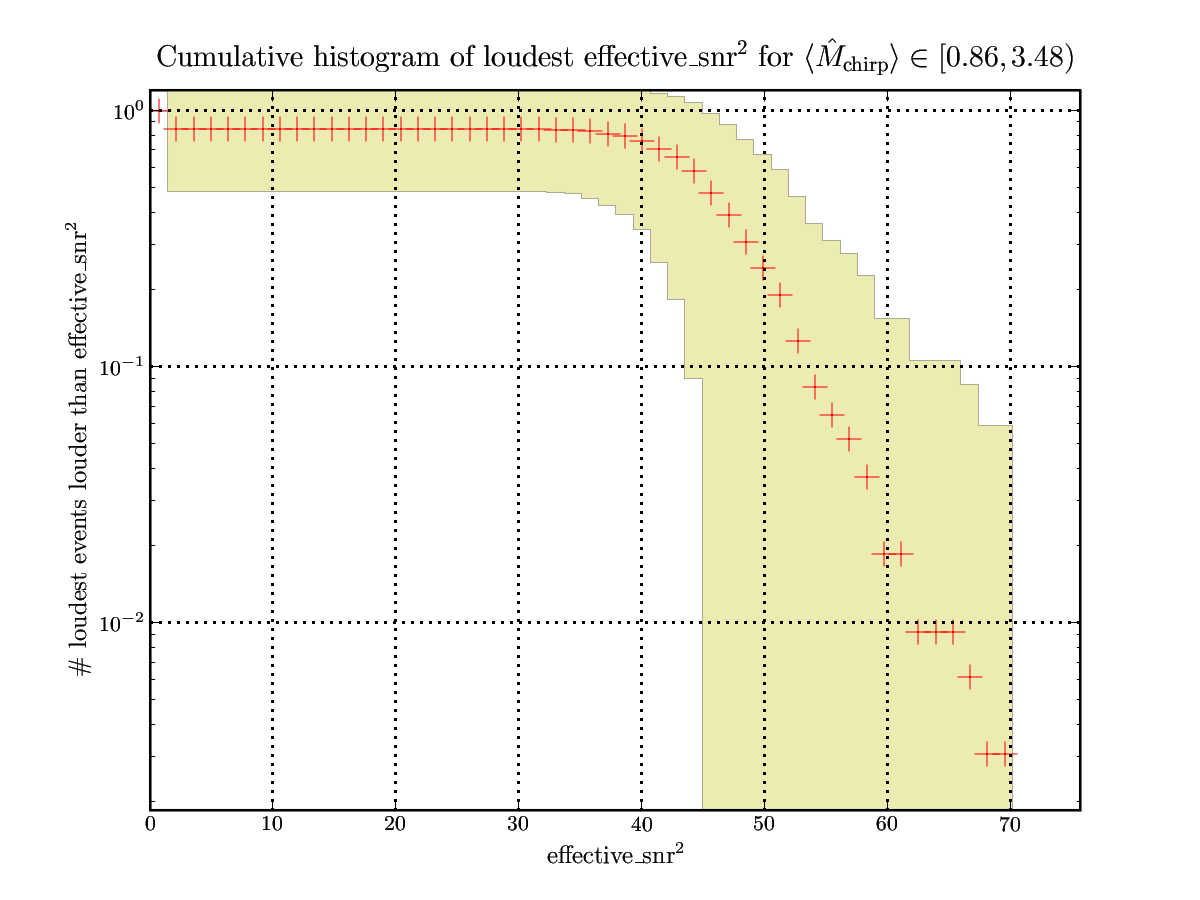
\includegraphics[scale=0.35]{Images/Triggers_Mc1.png}
\caption{Cumulative histogram of the loudest coincident triggers in low chirp mass bin versus combined effective SNR squared (proportion of triggers that have a combined effective squared SNR greater than or equal to a given value on the $x$--axis for the low chirp-mass bin). This represents the variation of the false alarm probability (FAP) with the ranking statistic. The FAP is constant and equal to 1 up to roughly an effective SNR squared of 40 corresponding to an individual detector SNR of $\approx4.5 - 5$, that is, triggers close to threshold. It then decreases linearly down to a value of one trigger per the total number of trials ($\approx$1/300) for a single trigger with a statistic of 70, corresponding to a single detector SNR of $\rho \approx 6 - 6.5$. This is the loudest background trigger and any on--source candidate, in order to represent a possible GW detection, should be as loud or louder}
\label{FARlowbin}
\end{figure}

The minimum non--zero false alarm rate one can get for an on--source candidate, louder than all the off--source loudest coincidences, bar one, is 1/(maximum number of trials = 324)$\approx3.1 \times 10^{-3}$ and, as will be seen in Chapter \ref{Chapter Five}, this is not enough for a detection statement. A more detailed explanation of the background estimation is given in Chapter \ref{Chapter Five}.

\subsection{Simulated signals}
\label{siminj}

There are two ways to test the pipeline's efficiency of detecting GW signals: by performing a large number of \emph{software injections} and by performing a much smaller number of \emph{hardware injections}. Software simulations are performed by adding a simulated waveform to the data after it has been read into the pipeline’s analysis codes; they cover a wide range of masses and coalescence times. Hardware simulations are performed by actually moving the detector mirrors (process called actuation) to mimic the effect of a possible GW signal. Hardware injections replicate more accurately a true GW signal, but are limited in choosing the injected parameters and only a limited number of these injections can be performed; data containing a hardware injection cannot be used when searching for real GW signals. Software injections are used in calculating the detection efficiency and the final upper limits. 

The search efficiency is defined as the fraction of simulated signals which are successfully detected by the pipeline. A software injection is considered found if there is a trigger found within 100 ms of the time of the simulation. This can lead to an injection being falsely found especially in the case when trigger rates are high; however, we are typically interested in evaluating the sensitivity of the search at or around the combined effective SNR of the most significant event -- in this case, the number of spuriously identified signals is essentially null. It is important, for tuning the analysis, to examine the simulations that \emph{should} have been found (given their amplitudes) but were not; since the amplitude is inversely proportional to the distance. simulations performed at low distances are still missed by the pipeline and one needs to find out the reasons why. Reasons for not finding an injection range from the existence of a very loud detector glitch at the time (or very nearby) of the injection, a very poor choice of parameters in the simulation (is mostly referred to high--spin simulations, in the case where we inject spinning waveforms, not applicable in our case). The missed/found injections plot for injections in H1 is shown in Figures \ref{injectionsH1} and \ref{injectionstimeH1}.

\begin{figure}[ht!]
\centering
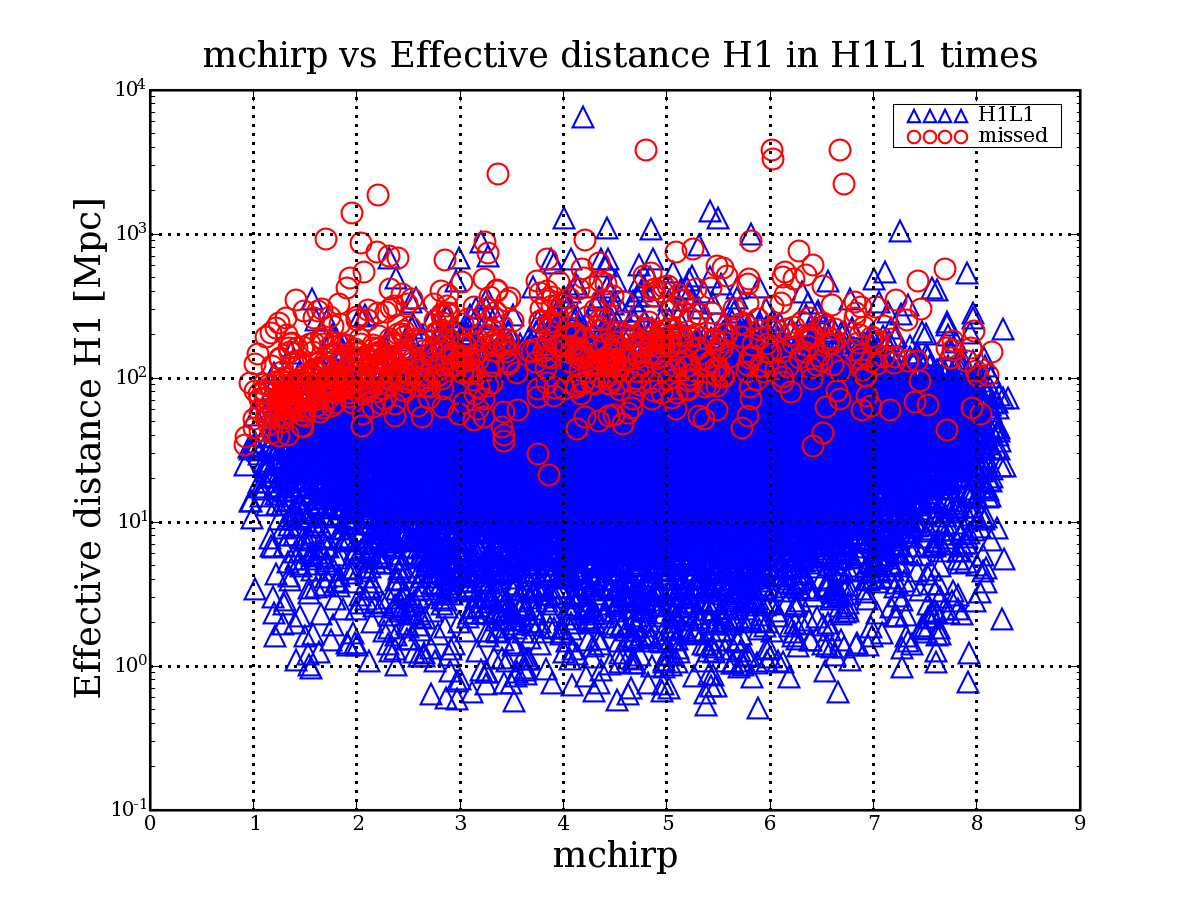
\includegraphics[scale=0.35]{Images/Foundmissed_INJ_H1.png}
\caption{Found/missed injections in H1: effective distance in Hanford H1 vs. chirp mass of found/missed simulations (blue triangles: found, red circles: missed). Injections with higher chirp mass tend to be found better since they have shorter templates that produce higher SNR triggers; the effective distance of a reference 1.4 -- 1.4 $\mathrm{M}_{\odot}$ binary at which we start missing injections is $\approx$40 Mpc, roughly the inspiral horizon distance in H1 (LIGO's H1 and L1 inspiral horizon distances at the time of GRB070429B were $\sim$35 Mpc for H1 and $\sim$34 Mpc for L1 respectively).}
\label{injectionsH1}
\end{figure}

\begin{figure}[ht!]
\centering
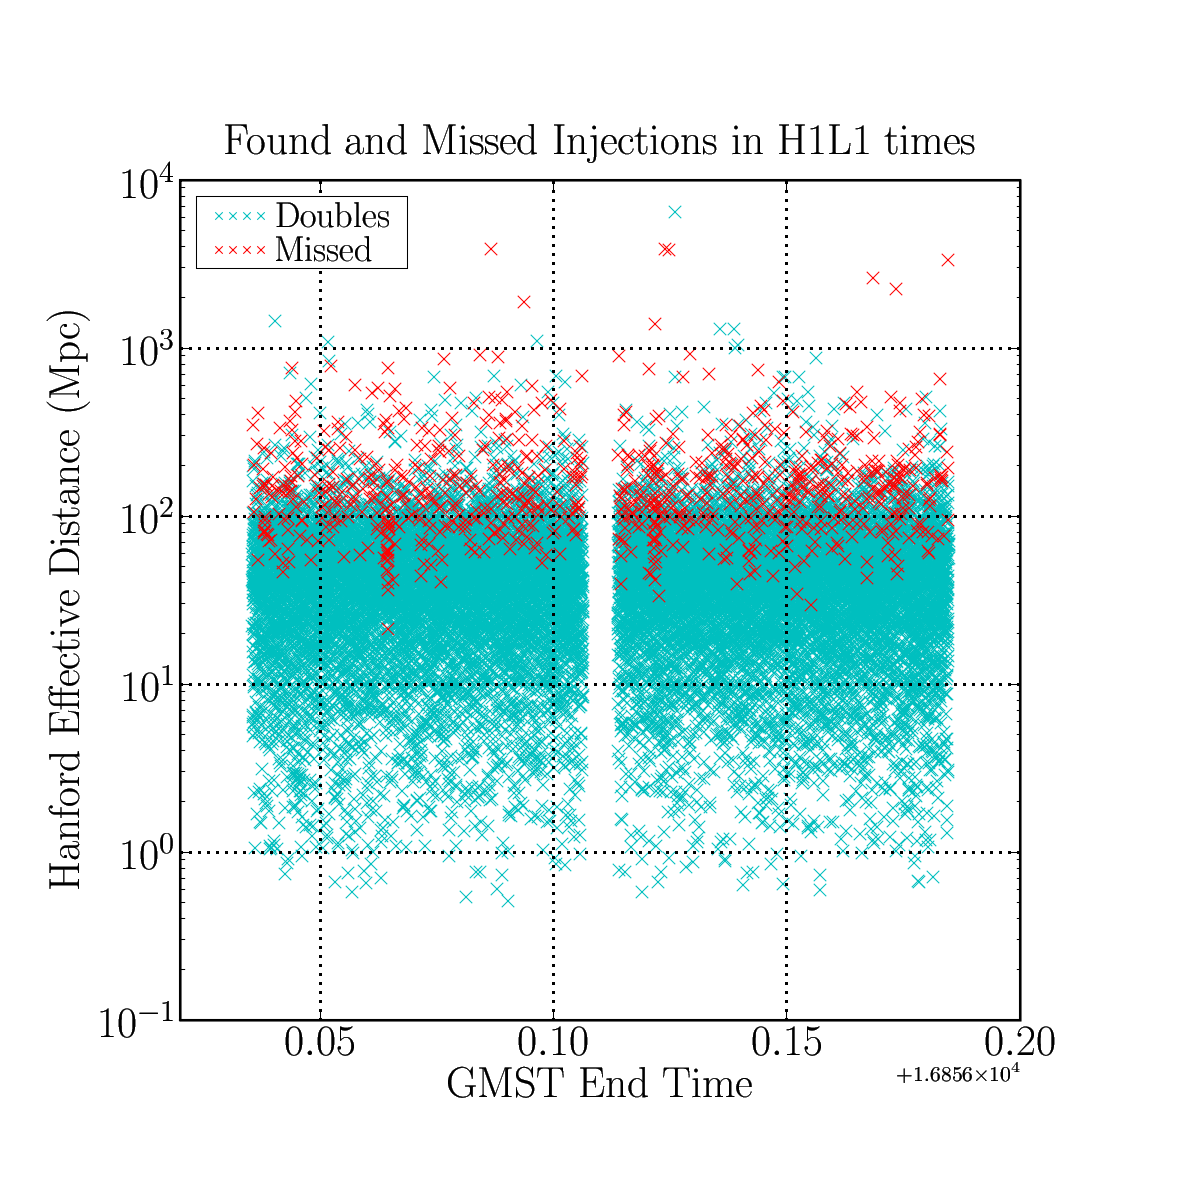
\includegraphics[scale=0.35]{Images/070429B_missed_time.png}
\caption{Found/missed injections in H1: effective distance in Hanford H1 vs. time. There are two times of poor data quality (``glitchy'' times) where injections are missed consistently at distances below the inspiral horizon distance, at 20--30 Mpc; we expect the fraction of missed/found injections to increase significantly at distances above 50 Mpc.}
\label{injectionstimeH1}
\end{figure}

It is important to cover the full search parameter space when performing simulations, both to test the analysis in order to find the cases where it doesn't perform as expected, and to accurately evaluate the sensitivity of the search. The simulations' parameter space is chosen depending on a set of astrophysical priors specific to the particular search we are performing. In the triggered search around short GRB times, we use the assumption that the progenitor source is a compact binary coalescence (either NS--NS or NS--BH binaries, see Chapter \ref{Chapter Two} for motivation) hence in terms of masses, we drew the NS mass uniformly from [1, 3) $\mathrm{M}_{\odot}$ and the BH mass uniformly from [1, 25) $\mathrm{M}_{\odot}$. We also restrict the parameter space by simulating signals only at the given sky location of the GRB (keeping dec constant and RA adjusted based on coalescence time $t_0$ to keep each simulation at the same location relative to the GW detector). In terms of inclination angle $\iota$ with respect to our line of sight, the simulations' $\iota$ was drawn uniformly in $\cos \iota$. The polarization angle was drawn uniformly in $[0,2\pi)$ and the coalescence time was uniform within the off--source time.

\subsection{Results: detection statement}
A simple ``poor man'' likelihood function is constructed to express how likely it is for an on--source candidate to be a signal (or not) -- we will derive a more precise expression of a detection likelihood in Chapter 5, using Bayesian inference; the likelihood is proportional to the pipeline efficiency in recovering simulated signals and inversely proportional with the background events false alarm probability:

\begin{equation}
\mathcal{L} := \frac{N_{\mathrm{found}}/N_{\mathrm{total}}}{N(\rho>\rho_0)/N_0}
\label{coinklike}
\end{equation}
%
where $N_{\mathrm{found}}/N_{\mathrm{total}}$ is the number of found injections divided by the total number of injections, or the injection recovery efficiency and $N(\rho>\rho_0)/N_0$ is the number of background events with an effective SNR $\rho$ larger than the onsource $\rho_0$, divided by the effective number of off--source trials, or the background FAP. The efficiency is a function of two signal parameters (distance and companion mass) and is marginalized over all other parameters; it is obtained by simply counting across injection trials. The FAP is obtained by counting across off-source trials. The FAP for every on--source candidate, for GRB070429B, is shown in Figure \ref{fig:far} and the low mass bin candidate, with an effective SNR=7.5 is the ``loudest'' on--source candidate but with a relatively high FAP=0.12, meaning it was only the $\approx$37th loudest candidate from on-- and off--source times collectively. The high chirp mass bin candidate, with FAP=0.117, is the most ``significant'' in terms of FAP, but only $\approx$35th loudest event of on-- and off--source collectively.

\begin{figure}[ht!]
\centering
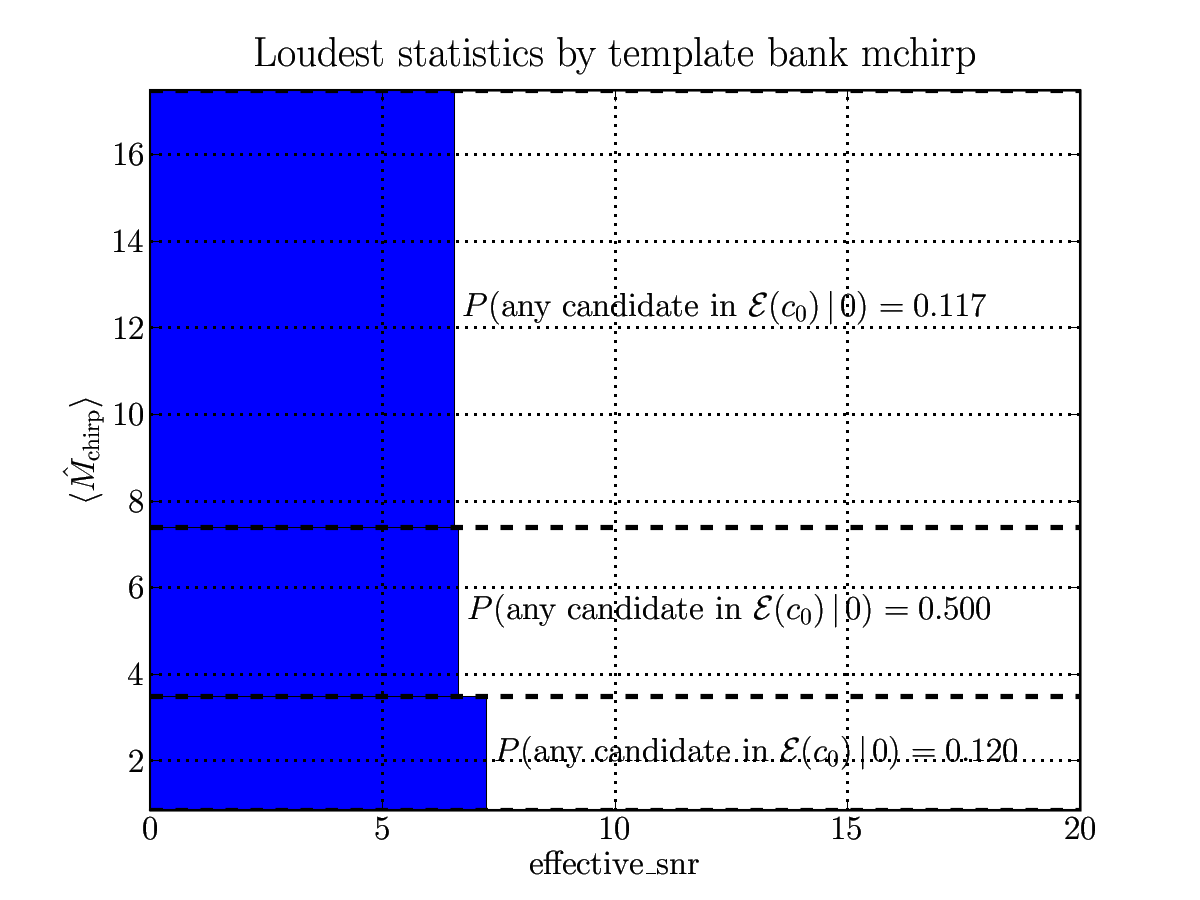
\includegraphics[scale=0.35]{Images/FAR.png}
\caption{False alarm probability for the on--source events in each chirp mass bin of GRB070429B, computed simply by counting the louder events in the background and dividing by the number of effective trials. The high chirp mass bin candidate, with FAP=0.117, is the most ``significant'' but only $\approx$35th loudest event of on-- and off--source collectively. The values on the $x$--axis correspond to the SNR of the loudest event in each of the chirp mass bins, plotted as solid bars on the $y$--axis.}
\label{fig:far}
\end{figure}

Figure \ref{onoffevents} shows the significance of the on--source loudest event relative to the distribution of background (off--source) events. The figure can be easily interpreted since the $x$--axis represents a statistic constructed from the likelihood given by equation \ref{coinklike}, that combines across the three chirp mass bins, and the $y$--axis is the event's probability of being drawn from the background sample -- this way we can see that the on--source event falls well in the background distribution and is not near the high--SNR ``tail'' of the rarest background events. In fact, to be able to claim a GW detection, the on--source event should be clear of the the background ``tail'', with false alarm probabilities of $\sim 10^{-6}$, as we will see in Chapter \ref{Chapter Five}, where we give an estimate for a FAP that should be associated with a GW--GRB detection.

\begin{figure}[ht!]
\centering
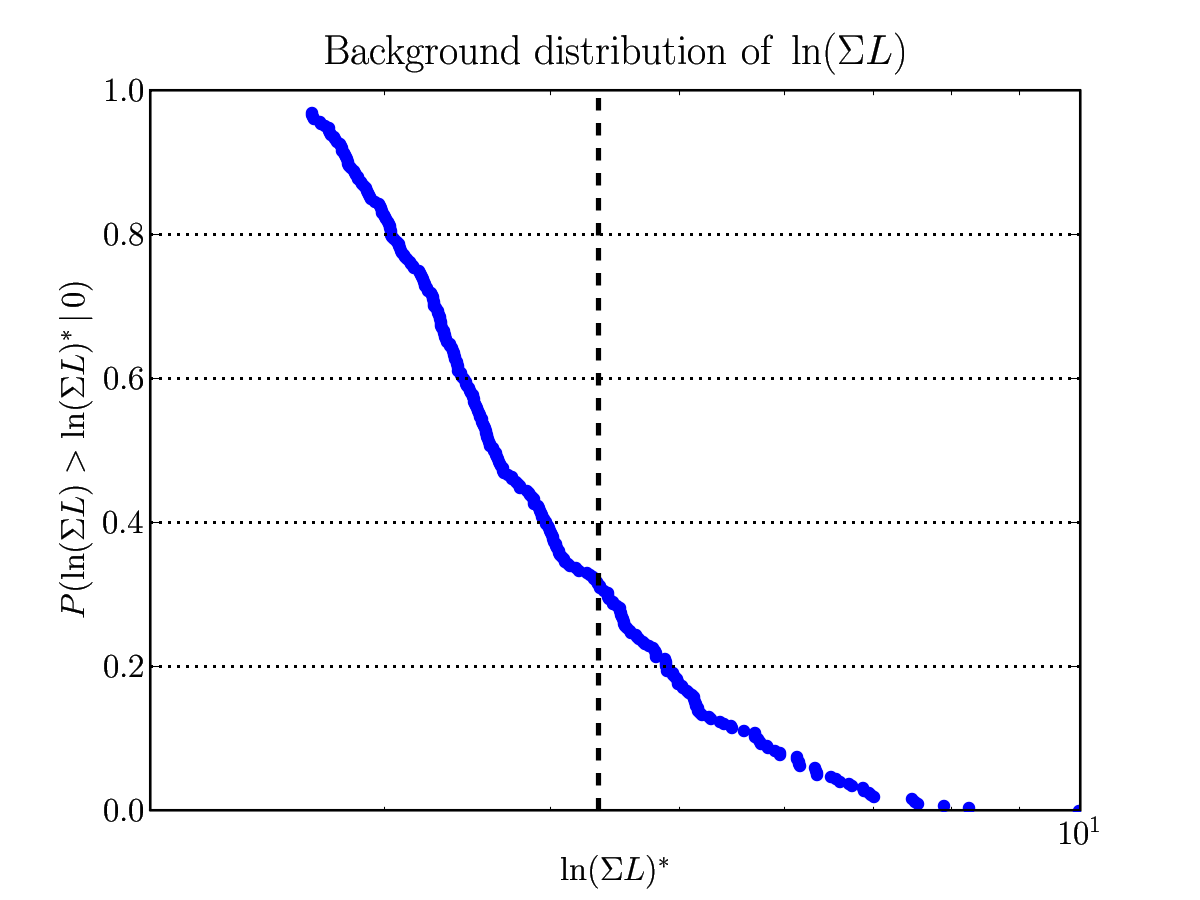
\includegraphics[scale=0.35]{Images/background.png}
\caption{The loudest on--source event (vertical dashed line) with respect to the background distribution of events (blue/dotted line). The figure can be easily interpreted since the $x$--axis represents a statistic constructed from the likelihood given by equation \ref{coinklike}, that combines across the three chirp mass bins, and the $y$--axis is the event's probability of being drawn from the background sample -- this way we can see that the on--source event falls well in the background distribution and is not near the high--SNR ``tail'' of the rarest background events..}
\label{onoffevents}
\end{figure}

\subsection{Results: distance exclusion}

Given the results from on--source, no detection of a GW signal was made. In this situation, we wish to place upper limits on the distance to the progenitor, based on the assumed astrophysical prior for the source: either a NS--NS or a NS--BH merger and the sensitivity of the search. We use the large number of simulations we performed and assume the GRB was caused by a compact binary coalescence with a neutron star (with a mass in the range [1, 3) $\mathrm{M}_{\odot}$) and a companion of mass $m_{comp}$. The $m_{comp}$ space is binned and we report a 90\% exclusion distance for a NS with mass in the range [1, 4) $\mathrm{M}_{\odot}$ and for BH with mass in the range [7, 10) $\mathrm{M}_{\odot}$. The actual computation of the exclusion distance will be omitted in this work but can be found in \cite{Abadie:2010uf}. We exclude a NS--NS merger to a distance of 9 Mpc and a NS--BH merger to 15 Mpc. These distances were derived assuming no beaming of the gamma radiation. The 90\% exclusion distance is larger for NS--BH systems than for NS--NS since more GW energy is radiated from a higher mass system; it also depends on the detectors' sensitivity (implicitly on the sky location of the GRB, see Chapter \ref{Chapter One}) and PSD at the time of the search, the likelihood of the on--source candidate(s) (if any) and on the parameter choice for simulations.


\subsection{Search summary}
We have analyzed 2190 s of GW data around the \emph{Swift} trigger time of the short hard GRB070429B. The two most sensitive operational GW detectors used for the search were H1 and L1. We have used the coincident triggered pipeline that looked for CBC signals using matched--filtering the data through a bank of theoretical waveforms. We have used two segments (one on either side of the GRB trigger) to estimate the background FAP and performed software simulations to obtain the search efficiency. We used a simple likelihood function (efficiency/FAP) to rank both on-- and off--source candidates. No gravitational wave signal has been detected in association with GRB070429B. The on--source data contains three triggers in each of the chirp mass bins but each of these triggers is not louder than the loudest background event; the most significant on--source trigger, in the high chirp mass bin, with an SNR of $\rho\approx$6.5 and a false alarm probability of FAP=0.12, was only order 30 loudest candidate from on-- and off--source times collectively. Given the GRB's association with a host galaxy at a luminosity distance of $\approx$4 Gpc, we would have not expected a GW detection. Based on the two astrophysical models for a CBC event (either NS--NS or NS--BH merger) we placed lower limits for distance to an NS--NS merger at 9 Mpc and for a NS--BH merger at 15 Mpc.

\section{Coherent triggered search}

\subsection{Introduction}

In Chapter \ref{Chapter Three} we have outlined the theoretical framework of a coherent analysis. In turn, in this section, we describe a triggered coherent search for \ac{CBC} signals associated with short GRBs and we will provide an example for illustration purposes. The particular search method, that we only summarize here, was used to analyze data during S6/VSR2 and 3 and is described in detail in \cite{Harry:2011qh} with search results in a final paper in the publication process \cite{lvc:s6grb}. This search was used to analyze \ac{GW} data around short gamma-ray burst triggers provided by both \emph{Swift} and Fermi/GBM satellites. Given the localization capabilities of the two GRB--observing missions, outlined in Chapter \ref{Chapter Two}, the search has been done on single sky points for the \emph{Swift}--observed GRBs (localization of arcsecond precision) and on multiple sky points within the Fermi--GBM error boxes (localization of a few square degrees precision). We will present here just a brief summary of this analysis method and of the results on GRB090831A, a GRB observed by the Fermi--GBM satellite. We invite the reader to consult the aforementioned references for an in--depth description of the coherent method and of the GRB analysis results for S6/VSR2 and 3. 

More recently, the same analysis method was used to analyze GW data associated with the IPN--detected short burst triggers collected during S5/VSR1. We will present in detail the search for GW associated with the S5/VSR1 IPN GRBs in Chapters \ref{Chapter Six} and \ref{Chapter Seven}.

The coherent analysis can be applied not only for single--point sky locations but also for extended sky regions, populated with multiple search points. A number of \ac{GRB}s that have been analyzed or to be analyzed, particularly those observed by Fermi--GBM and the InterPlanetary Network (see Chapters \ref{Chapter Two}, \ref{Chapter Six} and \ref{Chapter Seven}) are not localized with sufficient accuracy that the search could be done only at a single point on the sky.  Thus, the analysis has been extended to cover a region of the sky.  This requires looping over the relevant sky points, incorporating the correct detector sensitivities $F_{+,\times}$ and time delays between \ac{GW} detectors.  Since the majority of the analysis time is taken in performing the single detector filters and since these do \textit{not} need to be re--calculated for each sky point, the analysis does not take too much longer than the single--point one.  

Given the non--Gaussianity of the GW detector data and the lack of power of the matched--filtering to distinguish ``glitches'' from true signals, it is very important, on one hand, to understand the cause of these glitches \cite{Blackburn:2008ah} and to remove times of poor data quality. On the other hand, while the glitch--removal efforts greatly reduce the number of non--Gaussian events, they can not remove them entirely. Therefore the analysis must also employ methods to distinguish signal from noise transients. In previous \ac{CBC} searches, signal consistency tests e.g., \cite{Allen:2004gu, Hanna:2008} have proven very effective at removing the non--Gaussian background. We provided an overview of the formalism for the $\chi^{2}$ consistency test applied to coincident searches in Chapter \ref{Chapter Three} and in the previous section, and we will extend this test for the coherent analysis. This, together with describing new coherent--specific consistency tests such as the null stream and other multi--detector signal--based tests.

\subsection{Coherent search associated with GRB090831A}
\label{coh_search_grb}

\begin{figure}[ht!]
\centering
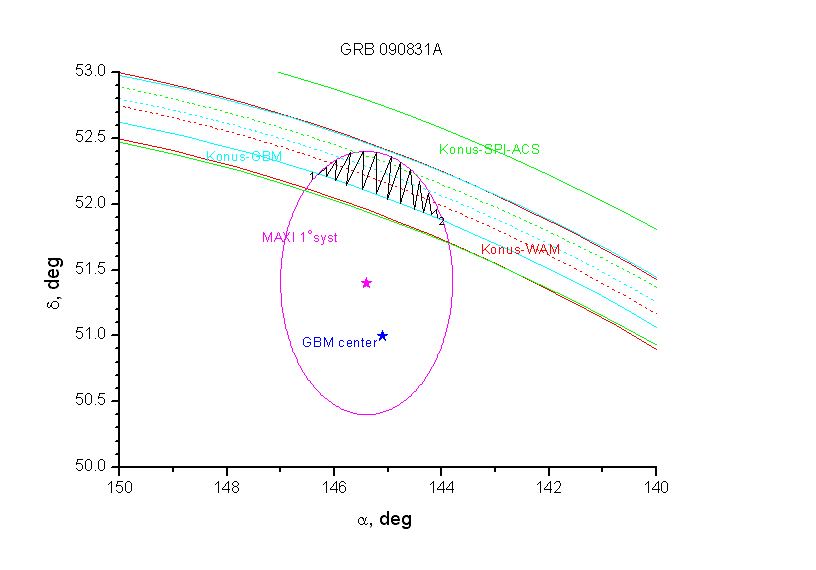
\includegraphics[scale=0.55]{Images/GRB090831A_IPN.png}
\caption{GRB090831A error region: blue star represents the Fermi--GBM localization error box best fit position; pink circle and star represent the MAXI (ISS) localization error box and best fit position, respectively; the hashed region represents the refined position with the help of IPN localization. The position accepted for the GW--GRB search was a conservative Fermi--GBM--only, centered at RA=145.1 and dec=51.0 degrees, with an error circle radius of $\approx$12.8 degrees -- figure from \cite{gcn9864}.}
\label{GRB090831A_IPN}
\end{figure}

\begin{table}[ht!]
 \begin{tabular}{|l|l|l|l|l|l|}
 \hline
 \hline
 GPS & Date & redshift & $T_{90}$ (s) & RA ($\deg$) & dec($\deg$) \\
 \hline
 935739411 & Aug. 31 2009, 07:36:36 UTC & n/a & 69 & 145.1 & 51.0 \\
 \hline
 \hline
 \end{tabular}
 \caption{Astronomical and detector data for GRB090831A. This was initially considered a long GRB/later considered short with an extended $T_{90}$ duration of $\approx$ 69 s and was observed by Fermi--GBM (and other missions, see text) to an approximate circular 1--$\sigma$ and systematics error box with a radius of 12.774 degrees. The active GW detectors were Hanford H1 and Virgo V1. Antenna factors are 0.146 and 0.881, respectively.}
 \label{Table_grb090831a}
\end{table}

\begin{figure}[ht!]
\centering
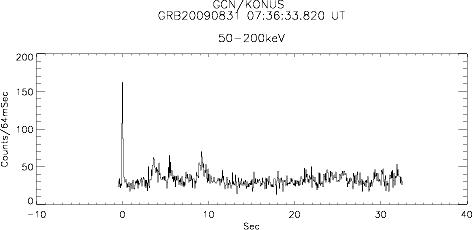
\includegraphics[scale=0.80]{Images/090831a_lc.png}
\caption{Konus--WIND GCN GRB090831A light curve (LC, $\gamma$ photon counts/s vs. time in the 50--200 keV band) showing a single intense peak followed by secondary and tertiary peaks. The $T_{90} \approx$69 s but this burst was still considered short based on visual inspection of this light curve \cite{konus}.}
\label{090831a_lc}
\end{figure}

\paragraph{GRB090831A overview}
GRB090831A is a \emph{long} gamma-ray burst detected initially by Fermi--GBM satellite and then by a series of other GRB missions. Based on subsequent visual inspection of the light curve, shown in Figure \ref{090831a_lc}, it was later considered \emph{short}, so a search for CBC events in association with it was ultimately performed. The light curve is showing a bright single peak followed by secondary and tertiary peaks. The Fermi--GBM light curve consists of two structured main pulses with a $T_{90}$ duration of about 69.1 s. According to GCN 9864 \cite{gcn9864}, GRB090831A was reported as both a Fermi--GBM and as a MAXI (Monitor of All-sky X--ray Image, an X--ray detector onboard the International Space Station, ISS) event. It was also reported as a Konus--WIND event, and detected by both Suzaku and INTEGRAL, both spacecraft part of the InterPlanetary Network (IPN, for further details on the the IPN and its missions, please consult Chapter \ref{Chapter Two} and Chapter \ref{Chapter Six}). Due to the involvement of the IPN in detection, the initial Fermi--GBM positional error region could be refined to a much smaller error box, see Figure ~\ref{GRB090831A_IPN} showing the Fermi--GBM best-fit position (blue star), the MAXI localization circle and best--fit position (pink star) together with the IPN (Konus--WIND, Suzaku, INTEGRAL) annuli (solid lines with centers dot--dashed). The hashed area shows the intersection of the Konus annulus with the 1--degree MAXI localization circle. The area of this region is 0.160 square degrees \cite{gcn9864}. Due to the fact that all Fermi--GBM--observed GRB locations are considered only based on the Fermi error circles, the position for the GW--GRB search was a conservative Fermi--GBM--only, centered at RA=145.1 and dec=51.0 degrees, with an error circle radius of $\approx$12.8 degrees (including systematic errors); we note that the IPN localization was available with a considerable delay, only after we have begun the GW search.

\begin{figure}[ht]
\centering
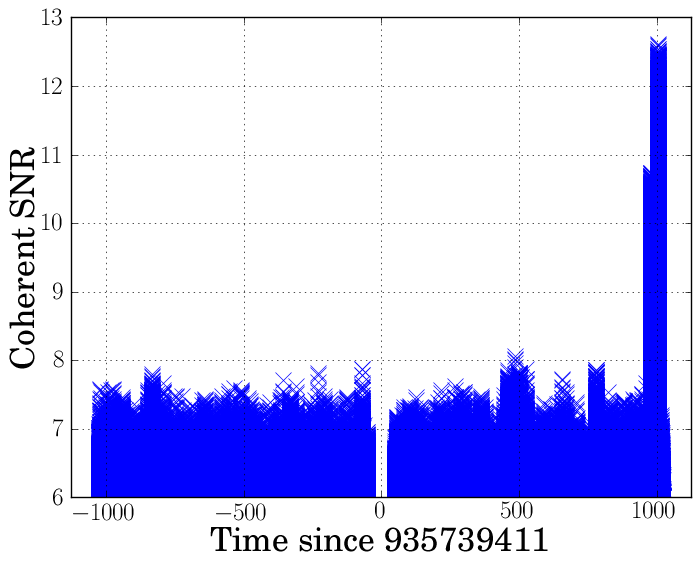
\includegraphics[scale=0.45]{Images/cohSNR.png}
\caption{The coherent SNR time series.}
\label{cohnull}
\end{figure}

\paragraph{Coherent SNR}
The coherent analysis uses the same data generation and matched--filtering procedures as the coincident analysis (already described for GRB070429B): 2190s of GW data was analyzed using H1 and V1 data. The coherent SNR is constructed from equation (\ref{eq:fstat_plus_cross}), from single detector SNR complex series, appropriately shifted and phased. In the analysis, the pipeline generates a trigger at any time for which the coherent SNR threshold is $\rho > 6$. Trigger clustering is done by only keeping the loudest trigger in each 0.1 s time interval.

\paragraph{Null--stream}
The null--stream is a powerful coherent--specific method of identifying and discarding noise transients that a coincident search would normally keep as possible signals. Since coherent SNR can be seen as a projection of coincident SNR on four components, the null--stream can be interpreted as the remainder of the coincident SNR that will not be projected and describes the noise, therefore we can write the null--stream statistic as the difference in quadrature of the coherent and coincident SNR:
%
\begin{equation}
\rho_{\mathrm{N}} = \sqrt{\rho_{\mathrm{coh}}^2 - \rho_{\mathrm{coinc}}^2}
\end{equation}
%
Given a coherent search that looks for signals in the $F_+$ and $F_{\cross}$ polarization channels, the null--stream is the third power channel that will be populated with noise--only transients. Ideally, a gravitational wave signal matching a template will provide no contribution to the null--stream and will be found only in either of the two other channels, so we expect that, for signals, the null--stream statistic will be $\chi^{2}$ distributed with $(2I - 4)$ degrees of freedom, with $I$ the number of detectors used for the search. A noise transient, on the other hand, that is incoherent across the data streams, may give a large coherent \ac{SNR}, but it is also likely to give a large null--stream statistic.

In the analysis, it is required that all events have an \ac{SNR} above 4 in the two most sensitive detectors in the network and the null--stream cut discards any event that has a null--stream statistic larger than $\rho_{\mathrm{N}} > 5.25$. Null streams are generated for analyses using data available from three or more GW detectors; in the case of our GRB, data from only two detectors was used, therefore no null stream was constructed.

\paragraph{Coherent $\chi^2$ test}
The main challenge to constructing a working coherent $\chi^2$ test is to choose the set of template waveforms $T^i$ to replicate the effect of glitches in the \ac{GW} data streams (see Chapter \ref{Chapter Three} and \cite{Harry:2011qh}). These are constructed by taking into account three factors: the waveform is accurate to a certain degree of precision, since the Post--Newtonian (PN) waveforms are derived from Taylor expansions that stop at a certain order \cite{Bliving} and the numerical waveforms suffer from similar inaccuracies \cite{Hannam:2009hh}; the template bank allows for some mismatch between the templates and any potential signal within the full parameter space to a maximal loss in SNR of 3\% \cite{OwenSathyaprakash98}; there are uncertainties in instrumental calibration \cite{Abadie:2010px} which will affect the match between signal and template.

We have described the theoretical framework for the single--detector $\chi^2$ test and application of the test to an analysis. For the multiple--detector test framework we invite the reader to consult \cite{Harry:2011qh}. A figure of the application of the $\chi^2$ test in reducing the numbers of background and injection triggers for GRB090831A can be found in Figure \ref{cohchi}.
%
\begin{figure}[ht]
\centering
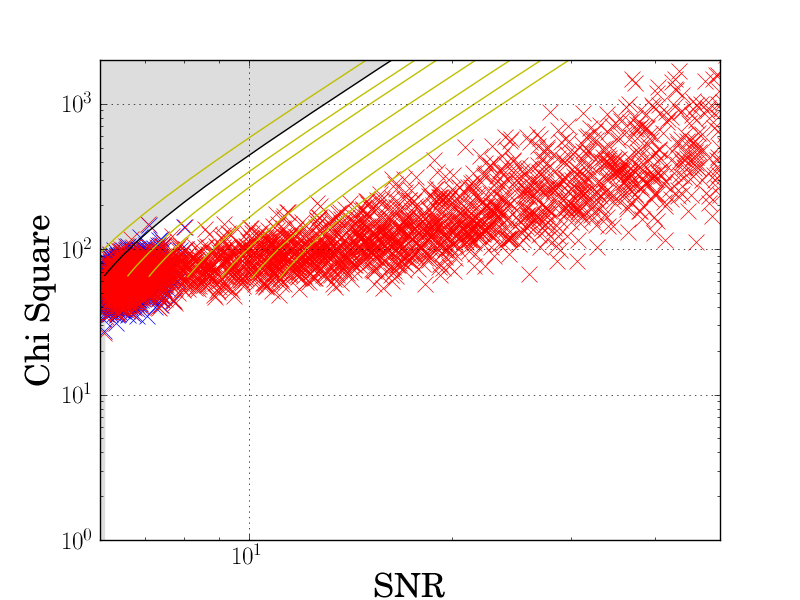
\includegraphics[scale=0.45]{Images/cohChi.png}
\caption{Coherent $\chi^2$ test applied to background (blue) and injection (red) triggers for the analysis of GRB090831A. The cut proves effective in eliminating about a quarter of the lower--SNR background triggers (SNR$\approx$6--7) and a few injections.}
\label{cohchi}
\end{figure}

\paragraph{Coherent bank $\chi^2$ test}
The coherent bank $\chi^2$ test has been conceived and implemented to test the consistency of the recovered SNR from a trigger across the waveform template bank. A \ac{GW} signal will match a certain number of templates giving a pre--described distribution of the SNR in the bank, whereas a glitch would produce numerous high--SNR events randomly distributed in the bank. The coherent bank $\chi^2$ test is calculated in the same manner as the regular $\chi^2$ test but instead it uses a fixed set of $N$ \ac{CBC} template waveforms $T^i$ which remain the same for every template $h(t)$ in the search template bank. These templates are taken from different points across the mass space and are well distributed across it.

For the bank $\chi^{2}$ to be efficient, glitches in the data must have a good overlap with a reasonable fraction of the templates $T^{i}$. While, in general, it is difficult to predict the composition of glitches in the data, it seems reasonable to assume that glitches which produce a large \ac{SNR} for the template $h(t)$ will also have a good overlap with other waveforms in the template space.  Thus, the set of templates which is spread across the parameter space is suitable. For further reference we ask the reader to consult \cite{Hanna:2008} and \cite{Harry:2011qh}.

An example of the application of the coherent bank $\chi^2$ test is shown in Figure ~\ref{cohbank} in the case of GRB090831A analysis.
%
\begin{figure}[ht]
\centering
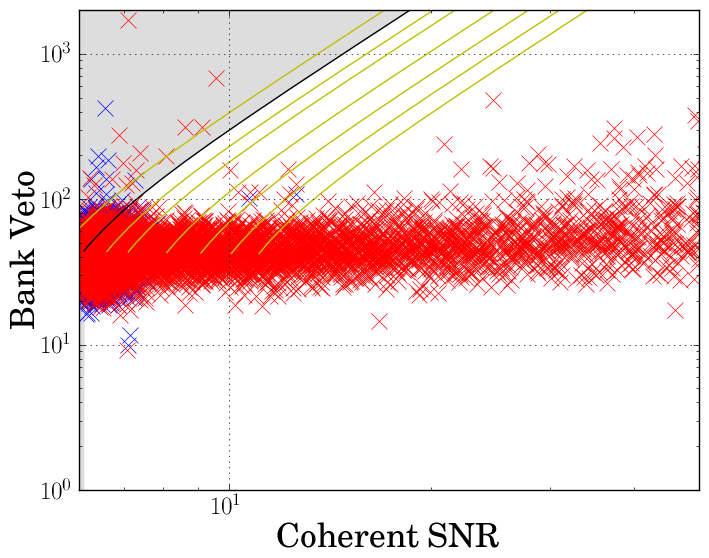
\includegraphics[scale=0.45]{Images/cohBank.png}
\caption{An example of the application of the coherent bank $\chi^2$ test is shown in the case of the GRB090831A analysis. We can see that this discriminator is powerful in this case, in removing background triggers (blue crosses) and a few low--SNR injections (red crosses). There is a number of background triggers close to threshold SNR that the test removes and a glitch at SNR$\approx$7 coincident with an injection, that the test misses.}
\label{cohbank}
\end{figure}
%

\paragraph{Coherent autocorrelation $\chi^2$ test}
Matched--filtering \ac{GW} detector data would produce SNR peaks for both real signals and glitches. The characteristics of a real signal time--series SNR peak differ from those of a glitch. The ``auto'' $\chi^{2}$ test was designed to test the consistency of the \ac{SNR} peak and was initially described in \cite{Hanna:2008}.  It is a similar test to the bank $\chi^{2}$, but if the bank $\chi^{2}$ investigates consistency in \ac{SNR} across the mass space, the auto $\chi^{2}$ tests for consistency of the \ac{SNR} time series.  The test uses the same search template bank containing waveforms $h(t)$ but applies a unique time difference $\Delta t$ of order of the template auto--correlation time , usually $<$0.01 s. Figure ~\ref{cohauto} shows the performance of the autocorrelation $\chi^2$ test in the case of the analysis of GRB090831A. Again, for further reference we ask the reader to consult \cite{Hanna:2008} and \cite{Harry:2011qh}.
%
\begin{figure}[ht]
\centering
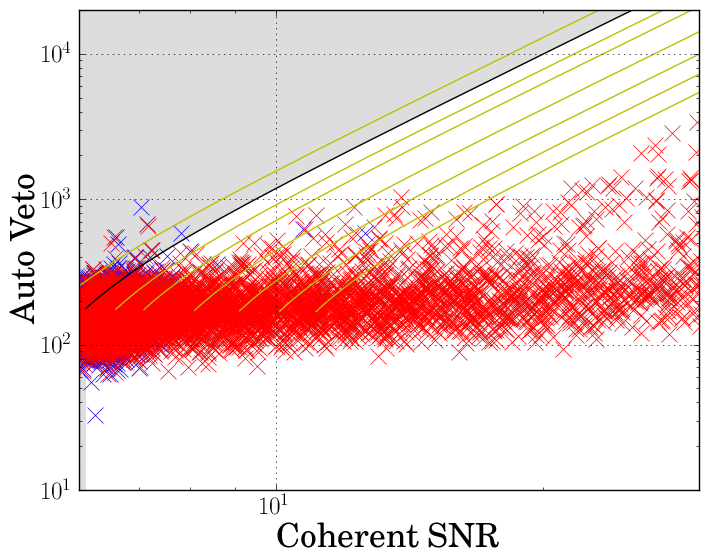
\includegraphics[scale=0.45]{Images/cohAuto.png}
\caption{The autocorrelation $\chi^2$ test for GRB090831A.}
\label{cohauto}
\end{figure}

\paragraph{Coherent background estimation}
After producing a coherent SNR time--series and applying the signal--based vetoes, described above, the analysis will rank the remaining triggers using a detection statistic constructed by using both the null--stream statistic $\rho_{\mathrm{N}}$ and the $\chi^2$ values for each trigger. This ranking statistic, defined as $\rho_{det}$ and given by
%
\begin{equation}\label{eq:rho_det}
\rho_{\mathrm{det}} =  \left\{
\begin{array}{ll}
 \displaystyle \rho_{\mathrm{new}} , & \rho_{N} \le 3.5 \\[0.1in]
 \displaystyle \frac{\rho_{\mathrm{new}}}{\rho_{\mathrm{N}} - 2.5} ,
 & 3.5 < \rho_{N} < 5.25 \, .
\end{array}
\right.
\end{equation}
%
where ``\textit{new SNR}'':
%
\begin{equation}
 \rho_{\mathrm{new}} = \left\{
\begin{array}{cl}
\displaystyle \rho, & \chi^2 \le n_{\mathrm{dof}} \\[0.1in]
\displaystyle \frac{\rho}{\left[\left(1 +
\left(\frac{\chi^2}{n_{\mathrm{dof}}}\right)^{4/3}\right)/2\right]^{1/4}}, & \chi^2 >
n_{\mathrm{dof}}
\end{array}
\right.
\end{equation}
%
where $\rho$ is the matched--filter trigger SNR. This detection statistic has the same expression as the ranking statistic used by the coincident analyses during S6/VSR2 and 3, and is a step forward from the S5/VSR1 effective SNR, with a better glitch rejection power at lower values of the $\chi^2$; $n_{\mathrm{dof}}$ represents the number of degrees of freedom for the $\chi^2$. The detection statistic is weighted by both the null--stream statistic and by the chi--squared values in order to improve the capacity of rejecting non--stationary noise triggers. Figure \ref{cohBG} shows the cumulative number of background events versus detection statistic in the coherent analysis of GRB090831A. By computing the background (off--source) trigger rate, expected purely from detector noise, we are able to assign a false alarm probability (FAP) to a possible detection event in the on--source 6s window. The false alarm probability is computed using the same formalism for the coincident search, and the detection (or non--detection) statement is made by quoting the results of equation:
%
\begin{equation}
\mathrm{FAP} = \frac {N(\rho>\rho_0)}{N_0}
\end{equation}
%
where the fraction is the number of background events with a coherent SNR $\rho$ larger than the onsource $\rho_0$, $N(\rho>\rho_0)$, divided by the effective number of off--source trials, $N_0$.

\begin{figure}[ht]
%\begin{minipage}[b]{0.5\linewidth}
%\centering
%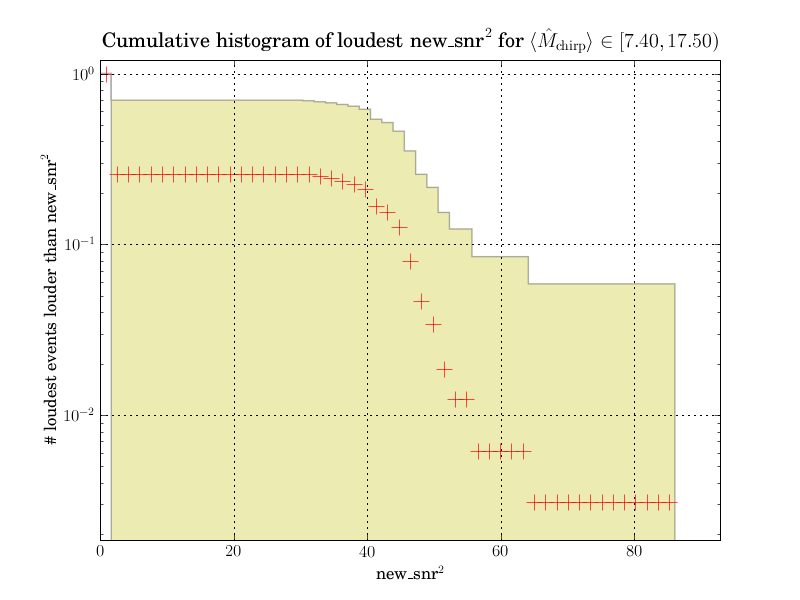
\includegraphics[scale=0.45]{Images/coincBG.png}
%\caption{Coincident analysis loudest background events in the high chirp mass bin. We can find notably more background events than in the coherent analysis of the same data; the maximum value of the detection statistic is $\approx$9.}
%\label{coincBG}
%\end{minipage}
%\hspace{0.5cm}
%\begin{minipage}[b]{0.5\linewidth}
\centering
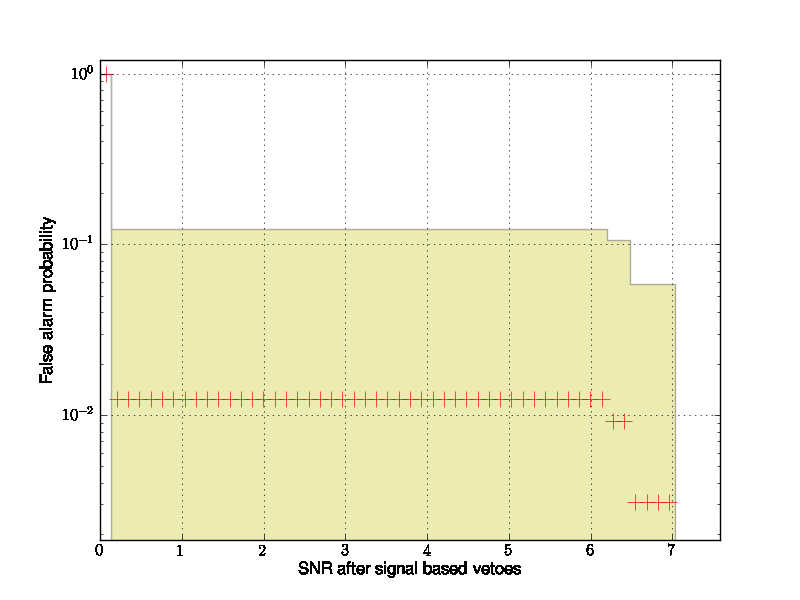
\includegraphics[scale=0.60]{Images/cohBG.png}
\caption{Coherent analysis loudest background events in the high chirp mass bin. We can find very few triggers that pass the signal--based vetoes and the maximum value for the detection statistic is $\approx$7.}
\label{cohBG}
%\end{minipage}
\end{figure}

\paragraph{Results: distance exclusion and search sensitivity}
No detection of a GW signal was made: a single event was found in the on--source in the low chirp mass bin with a FAP=0.71. In the case a GW signal detection is not made in association with the GRB, we would want to draw a set of parameters that characterize the search sensitivity. For each GRB we derive a 90\% confidence lower limit on the distance to the GRB progenitor for either the astrophysically--motivated NS--NS or NS--BH merger models. The method to determine this exclusion distance is further detailed in Chapter \ref{Chapter Seven}, where this is explained in light of the search for GW associated with the short hard GRBs detected by the IPN. Its application is the same here. In short, the 90\% exclusion distance is the distance where the efficiency of recovering injections (number of ``missed'' injections divided by number of ``found'' injections) drops below 90\%; or, it is the distance to which we are 90\% confident there was no CBC event associated with the particular analyzed GRB given the present search parameters (template bank, thresholds, signal--based vetoes, etc.). 

For GRB090831A the exclusion distance for NS--NS was 5 Mpc and for NS--BH, 9 Mpc. As a result of analyzing data around the 26 \emph{Swift} and Fermi--GBM short bursts during S6/VSR23, the median exclusion distance for NS--NS was 17 Mpc and for NS--BH, 29 Mpc \cite{lvc:s6grb}.

\section{Triggered searches: sensitivity improvement}
\label{sens_imprv}

We have presented two searches for GW associated with two short hard gamma-ray bursts; we used the GRB times and sky locations to perform triggered searches at the bursts' times and sky positions. It would be very useful to know how much we are gaining in sensitivity by doing a triggered search limited both in time (more generally, around the interesting electromagnetic transient, e.g., here the short GRB burst times) and in sky location (at the GRB right ascension and declination) as compared to an all--time, all--sky search. In this section we will estimate this increase in sensitivity by looking at different lengths of background data centered around the trigger time of our test GRB090809B and by comparing the background obtained from an untriggered (all--sky) search to the background obtained by performing a search at the sky location of the GRB. This will be just an estimation since to be able to get a decisive figure we will have to look not only at the background distribution but also at the simulations' recovery in the untriggered and triggered situations for multiple GRBs. We leave this for a future work.

To do this, we use the pipeline that searched for \ac{CBC} signals in an all--sky, all--time regime during S6/VSR23 (named ``ihope'', described in \cite{Abadie:2010yb, Colaboration:2011nz}). The pipeline looked for coincident events in each of the detectors that were available for the search and is, in broad lines, the untriggered equivalent of the coincident triggered pipeline described in Chapter \ref{Chapter Four}, Section ~\ref{coincident_GRB}. The reason we use ``ihope'' is that we need data from an untriggered search that is not available using the standard GRB pipeline and we need consistency (the same search method applied for different scenarios) to be able to compare results (just look at SNR values for fixed false alarm rates). The data was analyzed in four ways:

\begin{itemize}
\item
A week of data around the GRB090809B trigger time analyzed in all--sky, all--time regime (GPS 933895709, the analysis was performed between GPS 933379143 and 933984087). A histogram of the loudest background events in the zero--lag and timeslides (100 timeslides) is shown in Figure ~\ref{090809B_allsky_1week}. The ``loudest'' zero--lag event has an SNR$\approx$9.2 and the ``loudest'' timeslide event has an SNR$\approx$10.3. 

\begin{figure}[ht!]
\centering
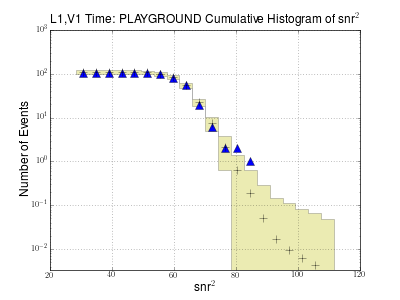
\includegraphics[scale=0.55]{Images/090809B_allsky_1week.png}
\caption{Histogram of the loudest background events in the zero--lag (triangles) and timeslides (100 timeslides, crosses) for a week of data around the GRB090809B trigger time, for an all--sky search. The ``loudest'' zero--lag event has an SNR$\approx$9.2 and the ``loudest'' timeslide event has an SNR$\approx$10.3. The analysis was made using the all--time, all--sky search pipeline (ihope, \cite{Abadie:2010yb, Colaboration:2011nz}).}
\label{090809B_allsky_1week}
\end{figure}

\item
A single day of data around the GRB090809B trigger time analyzed in all--sky, all--time regime (GPS 933895709, the analysis was performed between GPS 933852509 and 933938909). A histogram of the loudest background events in the zero--lag and timeslides (100 timeslides) is shown in Figure ~\ref{090809B_allsky_1day}. The ``loudest'' zero--lag event has an SNR$\approx$8.4 and the ``loudest'' timeslide event has an SNR$\approx$9.5.

\begin{figure}[ht!]
\centering
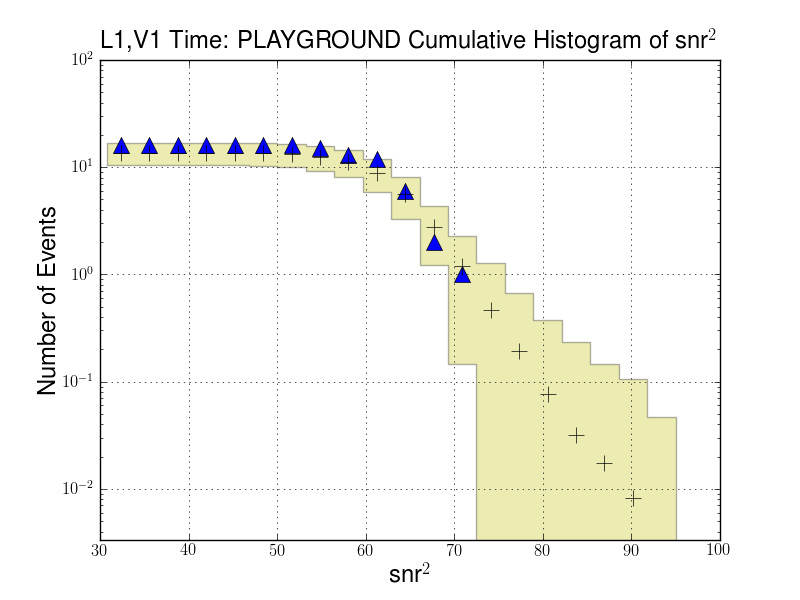
\includegraphics[scale=0.55]{Images/090809B_allsky_1day.png}
\caption{Histogram of the loudest background events in the zero--lag (triangles) and timeslides (100 timeslides, crosses) for a day of data around the GRB090809B trigger time, for an all--sky search. The ``loudest'' zero--lag event has an SNR$\approx$8.4 and the ``loudest'' timeslide event has an SNR$\approx$9.5. The analysis was made using the all--time, all--sky search pipeline (ihope, \cite{Abadie:2010yb, Colaboration:2011nz}).}
\label{090809B_allsky_1day}
\end{figure}

\item
2000 s of data around the GRB090809B trigger time analyzed in all--sky, all--time regime (GPS 933895709, the analysis was performed between GPS 933894709 and 933896709). A histogram of the loudest background events in the zero--lag and timeslides (100 timeslides) is shown in Figure ~\ref{090809B_allsky_2000s}. The ``loudest'' zero--lag event has an SNR$\approx$8.4 and the ``loudest'' timeslide event has an SNR$\approx$9.2.

\begin{figure}[ht!]
\centering
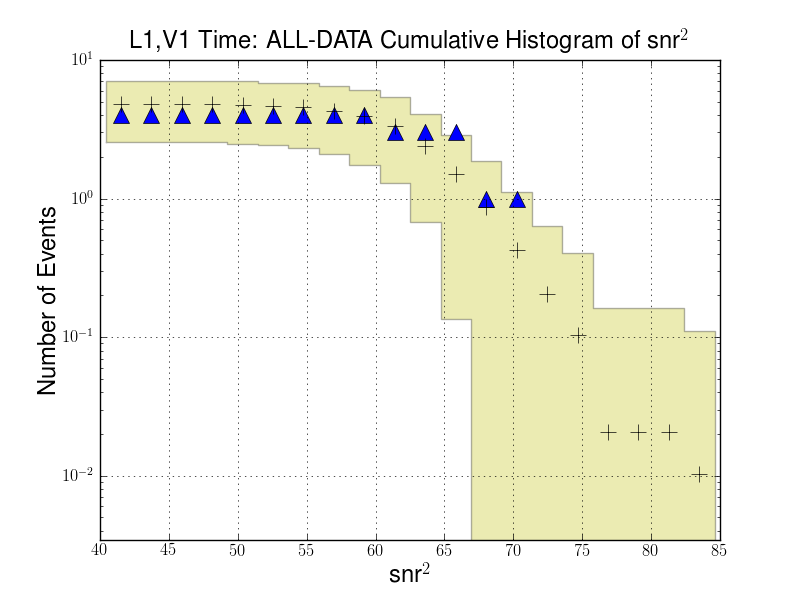
\includegraphics[scale=0.55]{Images/090809B_allsky_2000s.png}
\caption{Histogram of the loudest background events in the zero--lag (triangles) and timeslides (100 timeslides, crosses) for 2000 s of data around the GRB090809B trigger time, for an all--sky search. The ``loudest'' zero--lag event has an SNR$\approx$8.4 and the ``loudest'' timeslide event has an SNR$\approx$9.2. The analysis was made using the all--time, all--sky search pipeline (ihope, \cite{Abadie:2010yb, Colaboration:2011nz}) on a limited size data stretch.}
\label{090809B_allsky_2000s}
\end{figure}

\item
2000 s of data around the GRB090809B trigger time analyzed in triggered regime (GPS 933895709, the analysis was performed between GPS 933894709 and 933896709). A histogram of the loudest background events in the zero--lag and timeslides (100 timeslides) is shown in Figure ~\ref{090809B_directed_2000s}. The ``loudest'' zero--lag event has an SNR$\approx$7.9 and the ``loudest'' timeslide event has an SNR$\approx$8.6. The analysis was made by imposing condition on timedelays between operational detectors to search the the GRB sky location.

\begin{figure}[ht!]
\centering
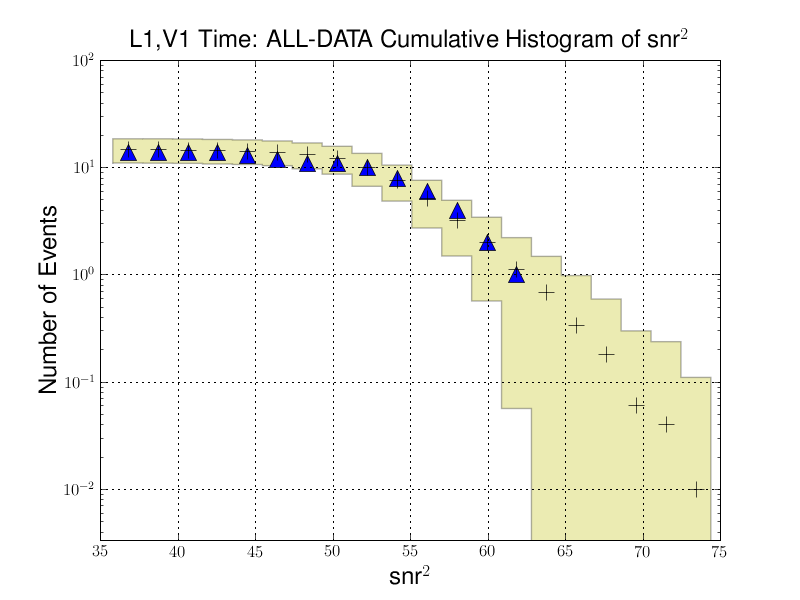
\includegraphics[scale=0.55]{Images/090809B_directed_2000s.png}
\caption{Histogram of the loudest background events in the zero--lag (triangles) and timeslides (100 timeslides, crosses) for 2000 s of data around the GRB090809B trigger time, for a triggered search at the sky location of the GRB. The ``loudest'' zero--lag event has an SNR$\approx$7.9 and the ``loudest'' timeslide event has an SNR$\approx$8.6. The analysis was made using the all--time, all--sky search pipeline (ihope, \cite{Abadie:2010yb, Colaboration:2011nz}) on a limited size data stretch imposing condition on timedelays between operational detectors to search the the GRB sky location.}
\label{090809B_directed_2000s}
\end{figure}

\end{itemize}

Suppose the data does not contain ``excessively loud'' glitches (previously removed by signal--based vetoes), and considering that the maximum SNR $\rho_{max}$ of the loudest event from the timeslid data (since a reliable background estimation can be done with timeslides only) at a fixed FAP and for the same search configuration in each of the cases above, characterizes the sensitivity of the search. The maximum SNR is a measure of how far in terms of distance can the search detect CBC events, relating to distance $\rho_{max} \propto 1/D_{max}$. We can estimate an increase of 13\% in sensitivity distance when reducing the analysis time from a week to 2000 s and another 7\% when using the sky location of the GRB for a triggered search. This amounts to approximately 20\% increase in sensitivity (distance) when comparing a week of analyzed data in all--time, all--sky regime with 2000 s of analyzed data in triggered regime on sky location. If we look at Figures \ref{090809B_allsky_1week} and \ref{090809B_allsky_1day} we notice that an event with effective SNR 90 will have a decrease in false alarm probability of order $7 \times 10^{-2}$ when shortening the analysis time from a week to a day, so roughly a measure of $10^{-2}$ FAP drop per day.

The 20\% increase in distance sensitivity translates into $\approx$73\% increase in volume sensitivity, which, in turn, assuming a naive constant number density for short GRBs, increases by $\approx$73\% the number of observable bursts.

These results are summarized in Table \ref{trig_untrig_comp}. Knowing the sky location of the GRB accounts for an increase of $\approx$7\% whereas knowing the exact time and being able to perform a search on a short stretch of data, without using a privileged sky location, increases the sensitivity by $\approx$13\% (1 week $\rightarrow$ 2000s), this shows that the major contribution to sensitivity increase from a triggered (time and sky location) search is knowing the exact trigger time. 

This estimation was performed using coincident data from \emph{two} GW detectors -- in the case of a triggered search using three or more detectors the sky localization will be improved (see Chapter \ref{Chapter One} for reference) therefore, the search sensitivity will increase as compared to the all--sky search. Further in--depth studies are needed, especially with the commissioning of Advanced LIGO, with trigger rates that are yet to be measured.

\begin{table}[ht!]
 \begin{tabular}{|l|l|l|l|l|}
 \hline
 \hline
 Case & FAP & $\rho_{max}$ & $D \propto 1/\rho_{max}$ & Sens. Increase (\%) \\
 \hline
 1 week ALL-SKY & $10^{-2}$ & 10.300 & 0.097 & n/a \\
 1 day ALL-SKY & $10^{-2}$ & 9.486 & 0.105 & 8\% \\
 2000s ALL-SKY & $10^{-2}$ & 9.110 & 0.110 & 4.8\% \\
 2000s TRIGGERED & $10^{-2}$ & 8.544 & 0.117 & 6.4\% \\
 \hline
 \hline
 \end{tabular} 
 \caption{Relative increases in search sensitivity for an identical search (same search parameters, using a single GRB trigger) performed on 1 week, 1 day and 2000s of data in all--sky mode and 2000s of data in typical GRB--triggered mode. $\rho{max}$ results are quoted at a fixed false alarm rate. Results suggest a typical increase of $\approx$20\% in sensitivity from a search on 1 week of data all--sky to 2000s triggered; knowing the sky location of the GRB accounts for an increase of 6.4\% whereas knowing the exact time and being able to perform a search on a short stretch of data increases the sensitivity by 12.8\% (1 week $\rightarrow$ 2000s).}
 \label{trig_untrig_comp}
\end{table}

\section{Discussion}

We have presented two different analysis methods to search for compact binary coalescences around short hard GRB triggers. Both methods have been used to produce results and publications: the coincident method was used in association with short GRB triggers during S5/VSR1 \cite{Abadie:2010uf} and the coherent method was used in association with short GRBs during S6/VSR2 and 3 \cite{lvc:s6grb}. Both methods make use of the sky location and time of the GRB event to gain search sensitivity as compared to all--time, all--sky searches. Both methods use matched--filtering the GW data through a set of theoretical waveforms (the ``template bank'') at their core, but the fundamental way of combining the data from multiple GW detectors differs. Whereas the coincident method looks for outstanding events that should be present in multiple detectors in the same time--chirp--mass window, the coherent method combines \emph{all} the data from \emph{all} the available GW detectors to extract two possible types of channels, a GW data channel and multiple noise channels (null streams). This, combined with a series of very strong signal--based veto tests, make the coherent search a more sensitive one compared to the coincident search.

We have presented search results from the coincident analysis associated with the \emph{Swift}--detected GRB070429B and coherent analysis associated with the Fermi--GBM--detected GRB090831A. No gravitational waves were detected in the 6s on--source window of any of these two short bursts. Therefore, we have computed a 90\% confidence distance to the GRB progenitor for the two predicted emission models (NS--NS or NS--BH).

We have also estimated the increase in sensitivity gained from performing a triggered search compared to an all--sky, all--time search. The sensitivity increase comes from both knowing the sky location and the time of the astrophysical trigger we wish to follow--up in GW data. This was done by successively comparing GW analyses that used data of different lengths and were performed either in all--sky or in triggered modes. W found an estimated 20\% sensitivity increase.

There still are ways to improve the current triggered search. One possibility would be an optimal choice for the detection statistic thresholds; another one would be better astrophysically--motivated priors on inclination or distance to the source.

This chapter was meant as a brief introduction to both coincident and coherent analysis methods and by no means as an in--depth study. For further reference to applying the coincident method to GRB triggered searches we invite the reader to consult \cite{Abadie:2010uf}; for the coherent application we point the reader to \cite{Harry:2010fr} and references therein.


\chapter{Improving searches for GW associated with GRBs} % Write in your own chapter title
\label{Chapter Five}
%\lhead{Chapter~\ref{ChapterLabel}
% \emph{Improving searches for GW associated with GRBs}} % Write in your own chapter title to set the page header
\section{Introduction}

The sensitivity of triggered searches for gravitational wave inspiral signals associated with short gamma-ray bursts may always be improved by implementing new data analysis techniques that increase the confidence of a possible detection; also, better knowledge of the source itself (astrophysical priors) may restrict the parameter space, making the analysis more sensitive and time and computing--efficient. In this chapter we describe such improvements for both the coincident and the coherent analysis methods: a better estimation of the background data using timeslides for a GW--GRB search and a proposed prior on the inclination angle of the binary.

Short hard gamma-ray bursts are cosmological events and are, on average, closer in luminosity distance than long gamma-ray bursts (see Chapter \ref{Chapter Two}), but those detected with the smallest measured redshifts are still beyond the inspiral range of present day GW detectors; however, this does not exclude the possibility of a future detection of a short burst with a much smaller redshift. Using a trigger from a GRB satellite and performing a GW search around this trigger is just the first step towards making a GW detection (see Chapter \ref{Chapter Four} for two examples of such searches); the second, and equally important part, is, in the case of finding an outstanding GW candidate associated with the GRB trigger, how confident we are that this candidate is indeed a gravitational wave and not arising from detector noise. 

Suppose we have this scenario: a short GRB is detected by a satellite and there is no afterglow that can identify a host galaxy, hence no information of its redshift or luminosity distance (see Chapter \ref{Chapter Two} for an explanation of short GRB afterglow detections). After performing a GW--GRB search one finds a loud (high--SNR) candidate associated with the GRB. The question arises: what is the false alarm probability that we should quote in order for us to claim a GW detection, with no supporting astrophysical information on the distance to the GRB in question? By ``false alarm probability'' we denote the probability that the newly found GW trigger \emph{is} produced by detector noise. This quantity is estimated purely from the statistical properties of the GW stretch of data that we analyzed and is a number we quote at the end of the analysis (see Chapter \ref{Chapter Four} for two such results). We will have to compare this number to an astrophysical quantity that gives information on the GRB. Such an astrophysical quantity would be the probability that the GRB was located at a luminosity distance within the GW detectors' range, and may be estimated from the collective properties of a population of short GRBs for which we know the distances. We describe two ways of estimating this probability.

We will look at a \emph{very} naive model for which we assume a constant number density for short GRBs within a physical spherical volume with a fixed radius of 2 Gpc ($z \approx 0.5$), in other words we consider that short GRBs occur only at very low redshifts. The 2 Gpc limit is chosen so the Euclidean and cosmological volumes are approximately equal. Assuming an optimistic average initial LIGO/Virgo horizon range of 20 Mpc for an ideally located and oriented NS--NS binary, we can express the probability that a certain given burst occurred within the detection volume for the GW detector:

\begin{equation}
\mathrm{P} = \frac{4\pi}{3}\frac{\mathrm{d}N_\mathrm{observable}(\mathrm{V_{detector}}=8 \times 10^{-6} ~\mathrm{Gpc}^3)}{\mathrm{d}N(\mathrm{V_{uniform}}= 8 ~\mathrm{Gpc}^3)} \approx 4 \times 10^{-6}
\label{grb_p}
\end{equation}

This is a very simplified way of estimating the chance that a GRB was within the GW detectors' range: short bursts are not proven to be uniformly distributed in volume (simply because we have not yet detected a very near--by one and the numbers of those with unambiguously determined redshifts are too small to derive any volume distribution); the GW detection range is not constant and depends on a series of parameters (binary localization and inclination, noise PSD etc., see Chapter \ref{Chapter Three} for reference); short bursts are not within redshift $z \approx 0.5$ only. Despite all this, the formula above gives a rough measure of this chance probability, estimated 1 in a million FAP.

A lower bound for the rate of observable short hard GRBs, $R$, approximated constant for the local universe, is given by the \emph{BATSE} short burst rate and is also the lower bound of the rate interval given by Nakar in \cite{Nakar:2007}:
%
\begin{equation}
R = 10~~~\mathrm{Gpc^{-3}yr^{-1}} = 10^{-8}~~~\mathrm{Mpc^{-3}yr^{-1}}
\end{equation}
%
This rate translates to $R\approx 10^{-4}~\mathrm{yr^{-1}}$ for short GRBs within initial LIGO detection range converted into a probability of $P\approx 5 \times 10^{-6}$. As mentioned in \cite{Nakar:2007}, this is the lower bound of the expected rate of observed short bursts, the upper bound possibly four orders of magnitude larger.

This probability expresses the chance that any of the observed short bursts in one year is located at a distance equal to or smaller than 20 Mpc, considered as average for initial GW detector range; this assuming, of course, that the observed GRB has no measured redshift from afterglow identification. Relating this to the false alarm rate and probability of a GW candidate, in order to claim an event detection, we can argue that it should be comparable with the chance probability of finding a short burst within a GW detector range distance. Quoting the two numbers above, the false alarm probability for a GW detection event should be larger than $\sim 10^{-6}$ for a confident detection statement.

\section{Background estimation using timeslides}

The search for the first GW signals from compact binary coalescences in detector data has so far faced a problem in estimating the significance of any candidate signal relative to the background of false events. This is because the detector data are non-stationary, in the sense of containing numerous, unpredictable and mostly unmodelled loud transients or detector ``glitches'', sometimes at high rates depending on the internal and external factors influencing the detector (see Chapter \ref{Chapter One} for non--stationary noise sources). If we consider searching for a well-defined waveform in noise by matched filtering, the distribution of the signal--to--noise ratio (SNR) in Gaussian data is completely predictable, thus the significance of a candidate signal with a given statistic follows immediately.

Many such non--Gaussian transients are removed by applying both a series of detector data quality checks (``vetoes'', that use information from a number of environmental channels such as seismic or electromagnetic disturbances, see Chapter \ref{Chapter One}) and a series of signal--consistency tests (e.g. the $\chi^2$-test, see Chapter \ref{Chapter Three} and previous chapter). But in real interferometer strain data, large glitch populations remain and dominate the distributions of candidate events at high detection statistic values, therefore we are unable to use a theoretical model of the statistical distribution for background. An example of estimating the significance of a GW detection candidate relative to the background data has been worked out with the occasion of the GW100916 ``Big Dog'' blind injection event and can be found in \cite{Colaboration:2011nz}.

We will present a method that estimates the background of a triggered GW search that uses timeshifting of individual detector data stretches. Since this method has been implemented and tested in the coincident search for CBC events, its theoretical framework depends on a few CBC search--specific parameters: coincidence window, individual detector trigger rates, false alarm probability derivation. We will estimate and make use of these parameters in the next paragraphs.


\subsection{Coincidence window estimation}

The coincident search looks for triggers within a certain coincidence window. A coincidence window $\delta v$, as explained in Chapter \ref{Chapter Three}, represents a bounded region in time in which we confirm that two or more triggers, from different GW detectors, are coincident. Estimating the background for a triggered GW search depends on the properties of the coincidence window: its size controls the number of coincidences. An optimal choice of its size will allow only a restricted number of single--detector triggers to pass the coincidence test (see the e-thinca threshold value in Chapter \ref{Chapter Four}); this will reduce the number of coincidences composed of single--detector ``glitches'' that tend to couple with near--threshold noise triggers. We will estimate the width of a coincidence window and use it in computing the false alarm probability. A fixed time--only coincidence window is the simplest coincidence window we can use and that takes into account only the coalescence times of each of the triggers; however, time--only coincidence windows prove inefficient in the case where two or more uncorrelated noise glitches are found within this window and their matching templates have different mass parameters.
 
Let's assume we have two triggers from two independent detectors with coalescence times $t_1$ and $t_2$; the detectors are separated geographically by a distance $d$. A time--only coincidence window is simply $\delta v = |t_1-t_2|$ and the maximum value of such a window is the ``light--travel'' time between the detectors: $\delta v \leq \frac{d}{c}$. Since we are dealing with noise (either Gaussian for an idealized model or non--Gaussian for actual data), this time is broadened to account for noise effects:
%
\begin{equation}
\delta v (\rho_0) \leq \frac{d}{c} + \frac{\alpha\sqrt{2}}{\rho_0}
\label{deltatro12}
\end{equation}
%
\noindent where $\alpha$ is a constant of order $\sim$ 100 ms \cite{Mukhopadhyay:2009qh} and $\rho_0$ is a chosen detection statistic threshold, usually $\rho_0 \approx 4.5 ~-~ 5.5$ in typical analyses. In the case of the triggered GRB search, where the sky location of the source is fixed, the light travel time $d/c$ is known \emph{a priori} so the second term of the sum in equation (\ref{deltatro12}) will be used only. Using these numbers we get a rough estimate for a time--only coincidence window $\delta v \approx 3 \times 10^{-2}$~s.

Since triggers should be coincident both in coalescence times and mass ($\tau_0$ and $\tau_3$ mass functions, for a definition of these variables see Chapter \ref{Chapter Three}), we would want to estimate the actual size of a time \emph{and} mass coincidence window as described in Chapter \ref{Chapter Three}, and applied in the coincident analysis in Chapter \ref{Chapter Four}. This will be done by using a three--dimensional rectangular window approximation, instead of the actual elliptical one, for ease of calculations. We again consider a pair of non--aligned detectors separated geographically by a distance $d$. In the standard analysis, three--dimensional coincidence \emph{elliptical} windows are used to find coincidences in both \emph{time of coalescence} $t_c$ and \emph{binary component masses}, $m_1$ and $m_2$ \cite{Robinson:2008un} encoded in by the $\tau_0$ and $\tau_3$ functions (see Chapter \ref{Chapter Three} for reference). Let's consider a three--dimensional rectangular coincidence window, with a volume $\delta^3 v_{\mathrm{r}}(\rho_0) = \delta v \Delta \tau_0 \Delta \tau_3$ given in \cite{Mukhopadhyay:2009qh}; the three--dimensional window will have a time--coincidence component $\delta v$ and two mass--coincidence components $\Delta \tau_0$ and $\Delta \tau_3$, each with time units. Then this is expressed as:
%
\begin{equation}
\delta^3 v_{\mathrm{r}}(\rho_0) = \delta v_{eff} \Delta \tau_0 \Delta \tau_3 \approx \frac{2\sqrt{2} \alpha a_{\tau_0}a_{\tau_3}}{\rho^3_0}
\label{rectum}
\end{equation}
%
\noindent where $\tau_0$ and $\tau_3$ are the two functions of binary component masses that define the template bank and $a_{\tau_0}$ and $a_{\tau_3}$ are two constants of order $\sim$2000 and $\sim$1000 ms respectively; the order of magnitude of $\Delta \tau_0$ and $\Delta \tau_3$ is $\sim$1000 ms \cite{Mukhopadhyay:2009qh}. Expressing an effective coincidence window, with time units:
%
\begin{equation}
\delta v_{eff}= \frac{2\sqrt{2} \alpha}{\rho^3_0} \left(\frac{a_{\tau_0}}{\Delta \tau_0} \right) \left(\frac{a_{\tau_3}}{\Delta \tau_3} \right)
\label{rectum2}
\end{equation}
%
and replacing the constants in equation (\ref{rectum2}) we get:
%
\begin{equation}
\delta v_{eff}(\rho_0) \approx \frac{4\sqrt{2}\alpha}{\rho^3_0}
\end{equation}
%
\noindent The volume of a corresponding elliptical coincidence window would be roughly one fifth of the rectangular one:
%
\begin{equation}
\delta v_{eff}(\rho_0) \approx \frac{4\sqrt{2}\alpha}{5\rho^3_0}
\label{xellipse}
\end{equation}

We obtain a rough estimate for the effective time--mass coincidence window $\delta v_{eff} \sim 10^{-3}$~s. The effective time--mass coincidence window is order $\frac{4}{5\rho^2_0} \approx 1/30$ the time--only window due to introducing the requirement of mass coincidence. Heuristically, by requiring mass coincidence, the chance of templates passing the coincidence test reduces by a factor of 30 to the case we require only a coincidence in time.

In the next sections we will be using two different coincidence windows for result comparison purposes: 

\begin{itemize}

\item
a fixed time and mass window that does not take into account variation on threshold SNR $\rho_0$, \emph{i.e.}, it is calculated at a fixed threshold $\rho_0 = 5$ $\rightarrow$ $\delta v = 10^{-3}$~s;
\item
a variable time and mass window that does take into account variation on threshold SNR $\rho_0$:

\begin{equation}
\delta v_{eff}(\rho_0) \approx \frac{0.11}{\rho^3_0}~~(\mathrm{s}).
\label{xellipse0}
\end{equation}

\end{itemize}


\subsection{False Alarm Probability}
One assumes that the single detector triggers with a detection statistic above a given threshold are uncorrelated realizations in time. Their distribution can be analytically approximated to a Poisson distribution with a constant occurrence rate. Analogously, one assumes that the distribution of coincidences formed by finding coincidences between individual detector triggers is Poisson as well. Let's assume we run an analysis over a stretch of time of length $T$. For simplicity, we will also assume the event rates (the rates at which triggers are produced in each of the detectors over time) $R_t$ can be considered constant. In this case, by $R_t$ we denote the \emph{single} detector trigger rate of a given detector. In practice, $R_t$ depends on the detectors' local noise characteristics (from time $t$ to time $t+\Delta t$ the detectors may experience a period of excessive non--Gaussian noise due to external factors like bad weather, human activity, earthquakes etc. hence increased trigger rates and consequently increased values for $R_t$). Therefore, the expected number of triggers will be $R_t T$ and the probability of obtaining $k$ triggers is given by the Poisson distribution:
%
\begin{equation}
p(k|R_t, T) = \frac{{(R_t T)}^k}{k!}\mathrm{e}^{-R_t T}
\label{PoissonApprox}
\end{equation}
%
Consider again the simplest case: we are looking for coincidences in data from two independent detectors with trigger rates $R_1$ and $R_2$, respectively. The search for coincidences is performed across a given coincidence window $\delta v$. The probability of having one or more coincidences in a coincidence window $\delta v$ provided the single detector trigger rates $R_1$ and $R_2$ (units triggers per second or Hz) and assuming the triggers are uncorrelated Poisson--distributed events, can be written \cite{Was:2009vh}:
%
\begin{equation}
\label{pr}
p(R_1, R_2) = p_1(R_1)p_2(R_2) = (1 - \mathrm{e}^{-R_1 \delta v})(1 - \mathrm{e}^{-R_2 \delta v}) \approx R_1R_2 \delta v^2
\end{equation}
%
by approximating $R_1 \delta v \sim R_2 \delta v \ll 1$; indeed this approximation is valid for typical single detector trigger rates of $\sim10-50$ Hz. Then, the average number of coincidences in time can be expressed as a rate:
%
\begin{equation}
R_c(R_1, R_2) = \frac{p(R_1, R_2)}{\delta v} \approx R_1R_2 \delta v
\label{far_c}
\end{equation}
%
with the associated Poisson error, given the only factors contributing to it are counting errors:
%
\begin{equation}
\sigma_c = \sqrt{\frac{R_1R_2\delta v}{T}}
\end{equation}
%

\subsubsection{Coincident GRB--GW search: frequentist FAP}

In assessing the significance of a coincident event produced by a given coincident GRB--GW analysis, the current method is to estimate the false alarm rate (FAR) or false alarm probability (FAP) which the event has when the analysis is run on a stretch of data that should not contain any GW signals henceforth called \emph{background}. The FAR can be defined as the rate of coincident events with a value of the detection statistic $\rho$ equal to or greater than the candidate event statistic $\rho_c$, in an analysis performed on the background data. If we apply the Poisson approximation then we obtain the probability of having at least one background coincident event, given an average coincidences rate $R_c$ and an analysis time $T$:
%
\begin{equation}
p(\mathrm{event}|R_c, T) = 1- p(0) = 1- \mathrm{e}^{-R_c T} \approx R_c T
\label{trueFAP}
\end{equation}
%
In the case of the GW--GRB analysis we use an ``on-source'' window of length $T$, where we perform the search for a possible GW signal, and $N_0$ independent ``off-source'' trials, each of length $T$ equal to the ``on--source'' window, considered background where there will be no expected GW signal from the analyzed GRB. Furthermore, it follows from equation (\ref{trueFAP}):
%
\begin{equation}
\label{peiN}
p(\mathrm{event}) = \frac{k_0}{N_0}
\end{equation}
%  
where $k_0$ is the total number of observed false alarms from all of the ``off--source'' trials $N_0$. This shows that the minimum nonzero FAP we can reach when having a background stretch of $N_0$ trials is for $k_0=1$, $\mathrm{FAP}_{min} = 1/N_0$. In a typical GW-GRB analysis the number of background trials is of order $N_0 \sim 300$, therefore the minimum nonzero will be FAP$\sim 3 \times 10^{-3}$. Comparing this to the probability that the GRB was within the detector range (equation (\ref{grb_p})), we see that we need to lower the FAP by several orders of magnitude in order to be confident of a detection.

\subsubsection{Coincident GRB--GW search: Bayesian FAP}

Using a Bayesian interpretation we can derive the false alarm probability considering that the observed false alarms $k_0$ are independent realizations distributed according to a binomial distribution. Suppose we treat the analysis as a series of independent trials; for each trial we retain the loudest coincident trigger and compare its SNR with the SNR of the ``on--source'' event -- if the trial coincident SNR is larger, then we call it a false alarm and count it in. Given $N_0$ trials, the probability distribution function for $k_0$ observed false alarms is the probability mass function:

\begin{equation}
P(k_0|q, N_0) = \frac{N_0!}{k_0!(N_0 - k_0)!} q^{k_0} \left (1-q \right )^{N_0-k_0}
\end{equation}

\noindent with $q$ the probability of obtaining a false alarm in one trial with boundaries [0,1]. 

From the Bayesian perspective, there are known and unknown quantities: the known quantity is the data, represented by the number of false alarms $k_0$ and number of trials background $N_0$; the unknown quantity is the probability $q$ for which we would want to derive the distribution function. To make inferences about the unknown quantities, we introduce a joint probability function that describes how we believe these quantities behave in conjunction, i.e., a probability density function (PDF) for $q$, $p(q|k_0,N_0)$, given $k_0,N_0$. Using Bayes’ rule, this joint probability function can be rearranged to get the PDF for $q$:

\begin{equation}		
p(q|k_0,N_0) = \frac{p(q) P(k_0,N_0|q)}{P(k_0,N_0)} = \frac{P(k_0,N_0|q)p(q)}{\int_0^1 P(k_0,N_0|q)p(q) \mathrm{d}q}
\end{equation}
%
Assume that $p(q)$ is a flat prior, i.e. $p(q)=1$, the denominator [0,1] bounded integral is solved by the incomplete beta function:
%
\begin{equation}
\int_0^1 P(k_0,N_0|q) \mathrm{d}q = \frac{N_0!}{k_0!(N_0 - k_0)!} B_q(k_0+1, N_0-k_0+1)
\end{equation}
%
and for $k_0$ and $N_0$ positive integers:
%
\begin{equation}
\frac{N_0!}{k_0!(N_0 - k_0)!} B_q(k_0+1, N_0-k_0+1) = \frac{1}{N_0+1}
\end{equation}
%
therefore the probability distribution function for $q$ will be:
%
\begin{equation}
p(q|k_0,N_0) = (N_0+1)P(k_0,N_0|q)p(q)=p(q)\frac{(N_0+1)!}{k_0!(N_0 - k_0)!} q^{k_0} \left (1-q \right )^{N_0-k_0}
\end{equation}
%
that should integrate to unity for a flat prior $p(q)=1$. We assume a flat prior on the event of interest (the ``on--source'' event) $p(q)=1$ (the probability of obtaining at least one event in the background louder than the ``on--source'') justified by the fact that there will always be an event in the ``on--source'' (as long as the SNR threshold is not set too high), so the distribution of $q$ is

\begin{equation}
p(q|k_0,N_0) = \frac{(N_0+1)!}{k_0!(N_0 - k_0)!} q^{k_0} \left (1-q \right )^{N_0-k_0}
\label{fap0b}
\end{equation}
%
The expected value for $q$ is
%
\begin{equation}
\mathrm{E}[q] = \frac{k_0+1}{N_0+2}
\end{equation}
%
the standard deviation is
%
\begin{equation}
\sigma^2 = \frac{(k_0+1)(N_0-k_0+1)}{(N_0+2)^2(N_0+3)}
\end{equation}
%
We notice that for small values of $k_0$ the error of $q$ is of the same order of magnitude as the value whereas for large values of $k_0$ the error converges to zero. A special case is $k_0=0$ (no background coincidence is louder than the ``on--source'' coincidence); in this case we have:
%
\begin{equation}
q = \frac{1}{N_0+2} \pm \frac{1}{N_0+2}\sqrt{\frac{N_0+1}{N_0+3}}
\end{equation}
%
The probability distribution function $p(q|k_0,N_0)$ has an extremum at
%
\begin{equation}
q_0 = \frac{k_0}{N_0}
\end{equation}
%
that is, in fact, the false alarm probability computed in the previous section using a frequentist approach (local extremum found by $\mathrm{d}p(q|k_0,N_0)/\mathrm{d}q = 0$).

The Bayesian approach to the false alarm probability gives us more information to it, that is, provides us not with a single frequentist extremum value but with a distribution function $p(q|k_0,N_0)$. This distribution is shown in Figure \ref{fap_distr} for a fixed number of trials $N_0=300$ and $k_0=1,2$, the case of a single background coincidence louder than the ``on--source'' and two such coincidences. We notice that the maximum FAP, $q_0$, will increase with $k_0$, as expected; we also note that the width of the distribution increases with $k_0$, in other words, the FAP computation becomes less precise for events with higher maximum FAP.

\begin{figure}[ht!]
\centering
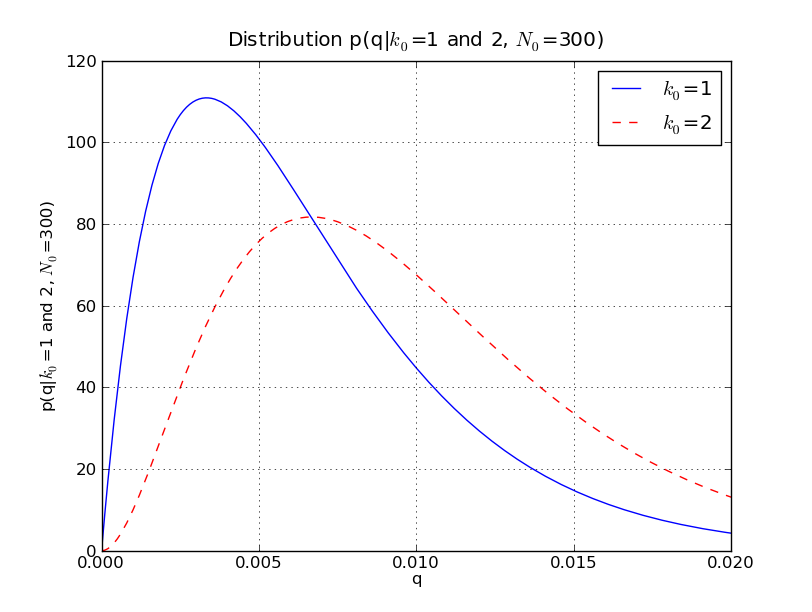
\includegraphics[scale=0.55]{Images/fap_distr.png}
\caption{Probability distribution function $p(q|k_0=1~\mathrm{and}~2,N_0=300)$ as a function of $q$. We notice that the maximum FAP, $q_0$, will increase with $k_0$, as expected; we also note that the width of the distribution increases with $k_0$, in other words, the FAP computation becomes less precise for events with higher maximum FAP.}
\label{fap_distr}
\end{figure}

\subsection{False Alarm Probability for $S$ Timeslides}

When prompted to assigning a certain false alarm probability to a candidate, one can artificially extend the background time, over which noise events can be gathered, by creating ``fake'' periods of data with approximately the same noise distribution as the real background data. This will keep the false alarm rate constant, but will allow us to make a more confident statement about a certain candidate by minimizing the error of the false alarm rate. This involves \emph{timesliding} the background data by a certain number of times, $S$, so that the new number of background trials will be $S \times N_0$. Physically, this is done by taking the detector data stretches and sequentially shifting one of them $S$ times by a certain amount of time $\Delta \tau$. By recombining the time--shifted data with the other non-slid segments, time--shifted triggers will form new coincident events. If the time--shifts $\Delta \tau$ are larger than the light travel time and the signal autocorrelation, then the time--shifted coincidences cannot be produced by gravitational waves, and are therefore expected to give a good estimate of the background -- from equation (\ref{far_c}) the coincidence rate is: 
%
\begin{equation}
\mathrm{FAR} = R_1R_2 \delta v
\label{thefar}
\end{equation}
%
and the variance will be, knowing that $S$ is the total number of timeslides, from \cite{Was:2009vh}:
%
\begin{equation}
\sigma = \sqrt{\sigma_{\mathrm{count}}^2 + \sigma_{\mathrm{recycled}}^2} = \sqrt{\frac{R_1R_2\delta v}{ST}+\frac{R_1R_2(R_1+R_2)\delta v^2}{T}}
\label{sigmatime}
\end{equation}
%
The first term of the sum represents ($\sigma_{\mathrm{count}}$) Poisson counting errors whereas the second term ($\sigma_{\mathrm{recycled}}$) represents the errors induced by repeating triggers forming different coincidences (``trigger recycling'', described in the following subsection). At low number of timeslides $S$, the counting errors will dominate the FAR error, whereas at higher $S$ values, the errors due to repeating triggers will dominate the magnitude of $\sigma$. This shows that the error will plateau if one increases the number of timeslides $S$ beyond a certain value, dependent on the single detector trigger rates $R_1$ and $R_2$ and the size of the coincidence window $\delta v$. In equation ~(\ref{sigmatime}), the number of timeslides at which the Poisson counting error term equals the repeating triggers error term:
%
\begin{equation}
\left ( \frac{R_1R_2\delta v}{ST} = \frac{R_1R_2(R_1+R_2)\delta v^2}{T} \right )_{S=S_{\mathrm{c}}}
\label{eq_saturation}
\end{equation}

\noindent will be improperly called the ceiling number of timeslides, $S_{\mathrm{c}}$. One may choose to do as many timeslides as one wants and there is no physical limit for $S$ simply imposed by the Poisson counting errors. It is just that by increasing the number of timeslides beyond $S_{\mathrm{c}}$ there is very limited gain in sensitivity. Hence, $S_{\mathrm{c}}$ follows from equation (\ref{eq_saturation}) and is given by:

\begin{equation}
S_{\mathrm{c}} = \frac{1}{(R_1+R_2) \delta v}
\label{timeslidesmax}
\end{equation}

By performing timeslides, we do not decrease the overall false alarm rate but rather decrease its error, compared to the case with no timeslides; the probability distribution function of the FAR will be peaked at the same maximum, but rather, the width will be smaller when doing timeslides.

GW detectors have different noise characteristics and local environmental influences, often resulting in very different trigger rates. It is useful to look at the accuracy of estimating the FAR when running an analysis with either very different detectors or similar ones, in terms of their individual trigger rates. We will be looking at equation (\ref{sigmatime}) that gives the FAR error $\sigma$ as a function of single detector trigger rates and number of timeslides and work with a constant FAR for both cases (it is only useful to assume a constant FAR to motivate a comparison of its error). Given two searches performed with two separate pairs of detectors, at a constant FAR and fixed number of timeslides $S$, we can differentiate two analysis cases: one that uses almost identical detectors, hence equal trigger rates $R_1 \approx R_2 = R$ and another that uses two very different detectors, with two very different trigger rates, e.g., $R_2 = f \times R_1$, where $f<1$ is an arbitrary proportionality factor. Since we are working at a fixed FAR, in equation (\ref{sigmatime}), the first term of the sum will be constant for both analyses, for the same number of $S$ timeslides. We need to compare the second term, namely $R_1+R_2 = (1+f) R_1$ with $2R$. We have the relation between $R_1$ and $R$, given a constant FAR: 
%
\begin{equation}
FAR = R_1R_2\delta v = fR_1^2 \delta v = R^2 \delta v
\end{equation}
%
hence $R=f^{1/2}R_1$. Replacing in equation (\ref{sigmatime}), we obtain the ratio of the two FAR errors in the two cases, for a fixed number of timeslides $S$:
%
\begin{equation}
\frac{\sigma_{R_1 \gg R_2}}{\sigma_{R_1=R_2=R}} = \sqrt{\frac{1+(1+f)SR_1 \delta v}{1+2\sqrt{f}SR_1 \delta v}}
\label{fractionalerror}
\end{equation}
%
For an arbitrary number of timeslides, e.g., $SR_1 \delta v=1$ (a low number of timeslides $S$=100, a relatively high trigger rate $R_1$=10 Hz and a typical estimated value $\delta v = 10^{-3}$ s), constant for both cases, we have the ratio as function of the proportionality factor $f$:
%
\begin{equation}
\frac{\sigma_{R_1 \gg R_2}}{\sigma_{R_1=R_2=R}} = \sqrt{\frac{1+(1+f)}{1+2\sqrt{f}}}
\end{equation}
%
For $f \rightarrow 0$ we expect an increase of roughly 50\% of the error on the false alarm rate when performing an analysis with two detectors with very different trigger rates as compared to one with similar trigger rates, for a given number of timeslides and a fixed FAR. In conclusion, the ability to measure the FAR is reduced when using two detectors with very different trigger rates; in such a case, we would be more susceptible to removing true signals, if present in the data. This effect is much enhanced when performing a considerable number of timeslides, e.g., of order $10^6$ (not applicable in the case of a GRB analysis where we have data stretches of only 2000s, but where we have longer data segments). In this case the dominant term will be $SR_1 \delta v$ of order $10^4$ and the ratio of FAR errors will be of order $(1+f)/(2 \sqrt{f}) \gg 1$ for small values of $f$. This effect is sensitive to values of single detector trigger rates: in the case of an analysis with very low trigger rates, e.g., $R_1 \approx 10^{-3}$, this effect may be neglected since $SR_1 \delta v \ll 1$ and the errors will be approximately equal: in equation (\ref{fractionalerror}) for small $f$ values the numerator and denominator sums will $\rightarrow$ 1.

To conclude, when dealing with relatively high single detector trigger rates, the timeslid background is better estimated (FAR error is smaller) when using data from detectors with similar trigger rates values, as opposed to very different trigger rates.

\subsection{Different scenarios for FAP and error}
\paragraph{Fixed time--mass coincidence window}
For a typical coincident GW--GRB analysis the single detector trigger rates close to threshold SNR are relatively high at values of order $R_1 \approx R_2 \approx 100$ triggers/second; using a constant coincidence window of order $\delta v \approx 10^{-3}$ s and a total number of trials $N_0 = 300$ with an ``on--source'' length of $T=6$~s, we can estimate what false alarm probabilities we would expect from three different classes of triggers, ranked solely by their characteristic SNR values (identical background triggers with different loudness): with low SNR, close to threshold, medium SNR and high SNR. Triggers with low SNR will have a high occurrence rate, whereas triggers with high SNR will have a low occurrence rate. Table \ref{xes} summarizes the false alarm rates and errors for these cases, for two types of analysis: without timeslides (``zero--lag'' only) and with S=100 timeslides. Trigger rates $R_1$ and $R_2$ are used in equations (\ref{thefar}) and (\ref{sigmatime}) to calculate the FAR and its error, $\sigma$; also in equation (\ref{timeslidesmax}) to estimate the ceiling number of timeslides, $S_{\mathrm{c}}$.

\begin{table}[ht!]
 \begin{tabular}{|l|l|l|l|l|l|}
 \hline
 \hline
 $R_1$ (Hz) & $R_2$ (Hz) & FAR (Hz) & $\sigma_{\mathrm{FAR}}$ (Hz) S=0 & $\sigma_{\mathrm{FAR}}$ (Hz) S=100 & $S_{\mathrm{c}}$ \\
 \hline
 100 & 100 & 10 & 1.3 & 0.60 & $<$1 \\
 10 & 10 & 0.1 & 0.13 & 0.02 & 50 \\
 1 & 100 & 0.1 & 0.13 & 0.04 & 10\\
 1 & 1 & 0.001 & 0.013 & 0.001 & 500 \\
 1 & $10^{-2}$ & $10^{-5}$ & $1.3 \times 10^{-3}$ & $1.3 \times 10^{-4}$ & $5 \times 10^3$ \\
 $10^{-2}$ & $10^{-2}$ & $10^{-7}$ & $1.3 \times 10^{-4}$ & $1.3 \times 10^{-5}$ & $5 \times 10^4$ \\
 $10^{-3}$ & $10^{-3}$ & $10^{-9}$ & $1.3 \times 10^{-5}$ & $1.3 \times 10^{-6}$ & $5 \times 10^5$ \\
 \hline
 \hline
 $R_1$ (Hz) & $R_2$ (Hz) & FAR (Hz) & $\sigma_{\mathrm{FAR}}$ (Hz) S=0 & $\sigma_{\mathrm{FAR}}$ (Hz) S=$10^3$ & $S_{\mathrm{c}}$ \\
 \hline
 $10^{-3}$ & $10^{-3}$ & $10^{-9}$ & $1.3 \times 10^{-5}$ & $1.3 \times 10^{-7}$ & $5 \times 10^5$ \\
 \hline
 \hline
 \end{tabular} 
 \caption{False alarm rates and their errors for different combinations of trigger rates for a simple two--detector analysis in the cases of ``zero--lag'' (no timeslides, S=0) and S=100 timeslides. Trigger rates $R_1$ and $R_2$ are used in equations (\ref{thefar}) and (\ref{sigmatime}) to calculate the FAR and its error, $\sigma$; also in equation (\ref{timeslidesmax}) to estimate the ceiling number of timeslides, $S_{\mathrm{c}}$. This illustrates the gain in confidence from a low--and--equal--trigger rates case. The very low trigger rates cases imply that the false alarm rate can be quoted only as a confidence interval [$-\sigma,\sigma$] that approaches [$-10^{-6}, 10^{-6}$] for trigger rates in the mHz region. We repeat the last row in the second section of the table; this is motivated by a choice of very low single detector trigger rates allowing the performance of a considerable amount of timesliding ($S=10^3$, permitted by equation (\ref{timeslidesmax})), in the case of an analyzed stretch of 2000 s, that, in turn, combined with very low and roughly equal single detector trigger rates (mHz), contribute to significantly lowering the $\sigma$ value of the FAR to reach $\approx 10^{-9}$ Hz and its error $\approx 10^{-7}$ Hz.}
 \label{xes}
\end{table}

By examining Table \ref{xes} we can draw a series of conclusions with regards to the usability of timeslides to estimate false alarm probabilities:
\begin{itemize}
\item
The coincidence rate for triggers with low SNR, close to threshold, is high and the timeslides method is indeed improving the FAR error but the large number of such coincidences would render any ``on--source'' trigger resembling them, completely insignificant. The FAR may have values of order 10 Hz and the ceiling number of timeslides is below 1, implying it is useless to do timeslides when we only have such triggers (see row 1 of the Table \ref{xes}).
\item
A factor contributing towards the increase of FAR error is two very different trigger rates in the two detectors, when dealing with relatively high trigger rates values (see rows 2 and 3 of the Table \ref{xes}). This effect is completely described by equation (\ref{fractionalerror}), that quantifies the fractional increase of the error for any given $S$ timeslides. The effect of two very different values for single detector trigger rates is of roughly 50\% increase in $\sigma$ for an analysis with a given $S$ timeslides and may increase significantly for analyses with much larger number of timeslides and high single detector trigger rates; note that for low $S$ and $R_1$, the effect is not so strong and the errors are approximately equal; also it suffices to consider the case of higher $S$ and not do a full analysis depending on the values of $S$ since a more exact background estimation for a GRB search will need higher values for $S$, i.e., $SR_1\delta v \gg 1$. The effect of two very different values for single detector trigger rates is less noticeable for low values of the single detector trigger rates, e.g., of order mHz, and relatively low number of timeslides. Ideally, an analysis should make use of two similar detectors in terms of trigger rates. This, combined with a low value of trigger rates, will allow for a smaller error value and for a larger number of usable timeslides.
\item
The coincidence rate for triggers with high SNR is low and in this case the timeslides method does improve the FAR error by an order of magnitude. Yet due to counting errors and repeating triggers, the error, even by performing 100 timeslides, is still of the same order of magnitude as the FAR (see row 4 of Table \ref{xes}).
\item
We can still achieve false alarm rates in the desired region of $10^{-6}-10^{-8}$ by performing timeslides if we have a very low individual detector trigger rate and the rates from any two detectors are comparable (at least of the same order of magnitude) (see rows 5,6 and 7 of the Table \ref{xes}; also the second section of Table \ref{xes}).
\end{itemize}

\subsection{Time--mass coincidence window function of threshold SNR}
As we see from Table \ref{xes} one would ideally want a very low trigger rate in the detector data. This can be achieved by very effective glitch--reduction procedures (effective detector characterization), very strong signal--based vetoes and by raising the SNR threshold. Glitch--rejection and signal--based vetoes tend to reduce the number of loud noise events and not to reduce the background of near--threshold ones. We will briefly discuss the third option: raising the SNR threshold $\rho_0$ that will significantly reduce the number of low--SNR noise events. Using equation (\ref{xellipse0}), we can write the FAR and its error as a function of threshold SNR $\rho_0$:
%
\begin{equation}
FAR(\rho_0) = \frac{0.11R_1R_2}{\rho_0^3}
\end{equation}
%
and
%
\begin{equation}
\sigma = \sqrt{\frac{0.11R_1R_2}{ST\rho_0^3}+\frac{10^{-2}R_1R_2(R_1+R_2)}{T\rho_0^6}}
\end{equation}
%
Also, suppose we assume, in a very approximate case, that the single detector trigger rates are equal and decrease as exponential functions of threshold SNR:
%
\begin{equation}
R_1 \approx R_2 \approx C\mathrm{e}^{-\alpha \rho_0}
\end{equation}
%
where $C$ and $\alpha$ are two analysis--dependent constants that we can evaluate and approximate fixed for similar analyses. This naive approximation is not very far from reality in the ideal case of a stretch of data without any major non--Gaussian noise activity. The constant $C$ can be evaluated using the trigger numbers from Chapter \ref{Chapter Four} for the case of GRB090809B: at a threshold SNR $\rho_0=4.5$ the single detector trigger rates were in the region of 50 Hz, giving us an estimate $C=3 \times 10^{10}$ Hz. The constant $\alpha$ can be evaluated knowing that there is order 100 drop in FAR for a unit increase in SNR, so roughly $100 \approx \mathrm{e}^{\alpha}$, giving $\alpha \approx 4.5$. This way we can re--write both the FAR and its error taking this into account:
%
\begin{equation}
FAR(\rho_0) = 9 \times 10^{18} \times \frac{\mathrm{e}^{-2 \alpha \rho_0}}{\rho_0^3}
\end{equation}
%
and
%
\begin{equation}
\sigma = 3 \times 10^9 \times \sqrt{\frac{\mathrm{e}^{-2 \alpha \rho_0}}{ST\rho_0^3}+6 \times 10^{10}\frac{\mathrm{e}^{-3 \alpha \rho_0}}{T\rho_0^6}}
\end{equation}
%
with a ceiling number of timeslides as a function of threshold SNR:
%
\begin{equation}
S_c \approx 1.7 \times 10^{-11}\rho_0^3\mathrm{e}^{\alpha \rho_0}
\end{equation}
%
The false alarm rate and its error are shown in Figure \ref{FAR_threshold}: false alarm rate variation with threshold SNR $\rho_0$ (continuous line) and its error (dashed lines) for $T=6$ s and a sequence of $S=10^n$ timeslides where $n=\bar{0,11}$; vertical lines corresponding to a sequence of $\rho_0$=5, 6, 7, 8 and 9, in a log--log plot. The dashed contours representing the $\sigma$ of the FAR, for constant number of timeslides, reveal two very important findings: the error saturates and does not decrease anymore even if we would perform an infinite number of timeslides (this was also shown in equation (\ref{eq_saturation}), explaining the existence of a ceiling number of timeslides, above which there is no decrease in error); and justifies the performance of timeslides in order to obtain a reduced error on the false alarm rate: the error decreases with increasing $S$.

\begin{figure}[ht!]
%\begin{minipage}[b]{0.5\linewidth}
\centering
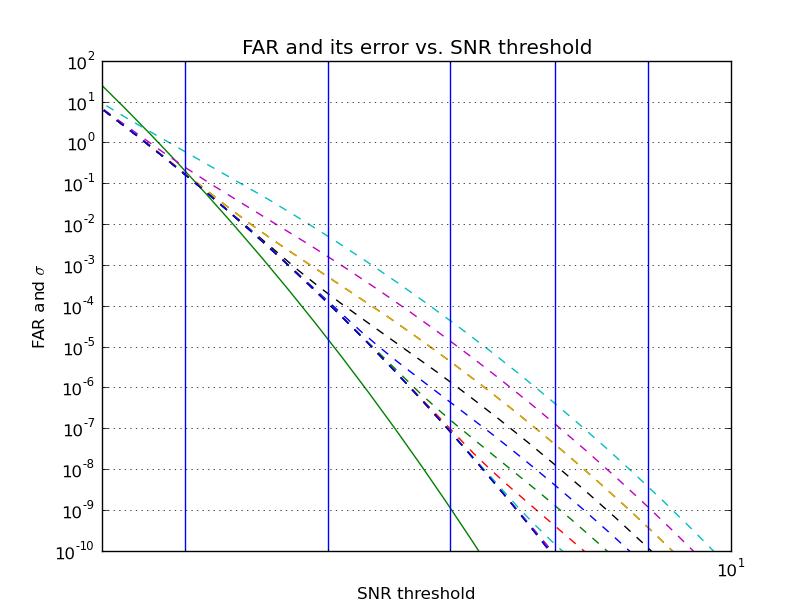
\includegraphics[scale=0.55]{Images/far_threshold1.png}
\caption{False alarm rate variation with threshold SNR $\rho_0$ (continuous line) and its error (dashed lines) for $T=6$ s and a sequence of $S=10^n$ timeslides where $n=\bar{0,11}$, the furthest error line from the FAR line is for $n=0$ and the closest for $n=11$; vertical lines corresponding to $\rho_0$=5,6,7,8 and 9, log--log plot. The dashed contours representing the $\sigma$ of the FAR, for constant number of timeslides, reveal two very important findings: the error saturates and does not decrease anymore even if we would perform an infinite number of timeslides (this was also mentioned in equation (\ref{eq_saturation}), explaining the existence of a ceiling number of timeslides, above which there is no decrease in error); and justifies the performance of timeslides in order obtain a reduced error on the false alarm rate: the error decreases with increasing $S$.}
\label{FAR_threshold}
%\end{minipage}
%\hspace{0.5cm}
%\begin{minipage}[b]{0.5\linewidth}
%\centering
%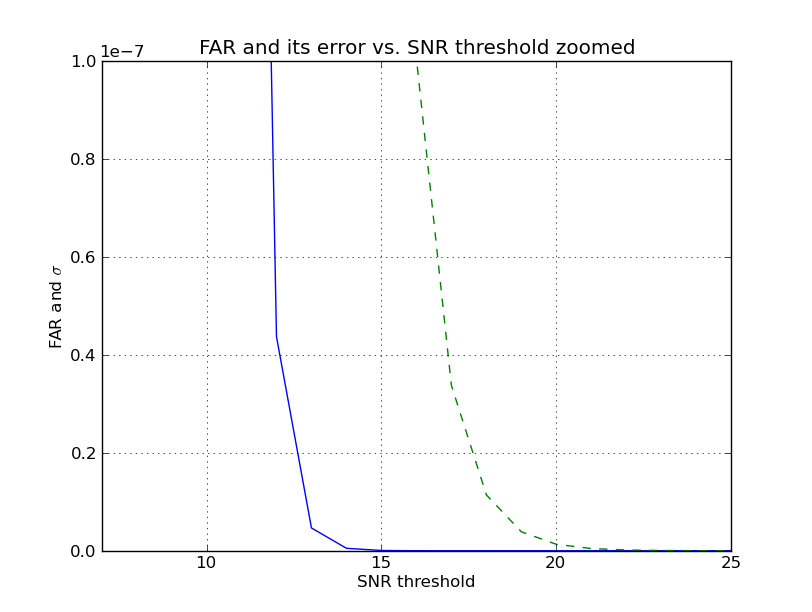
\includegraphics[scale=0.40]{Images/FAR_threshold_zoom.png}
%\caption{False alarm rate variation with threshold SNR (continuous line) and its error (dashed line) in the region of interest for the FAR of a GW--GRB search. The error is roughly two orders of magnitude larger than the FAR.}
%\label{FAR_threshold_zoom}
%\end{minipage}
\end{figure}

Looking at a practical case: suppose we impose a threshold SNR $\rho_0=7$, or consequently, we have two coincident triggers, each with SNR's 7 -- this would mean an effective SNR of $\approx$10, which would probably mean the loudest event in the case of a GW--GRB search. The coincident event will have a FAR$\approx 10^{-9}$ and the error on the FAR will be $\sigma \approx 10^{-4}$ for S=1 timeslides (``zero--lag''+1 slide only) and $\sigma \approx 10^{-7}$ for S=$10^3$ timeslides (possible for a 2000 s data stretch), already becoming of interest given the very low probability of finding a short GRB located within the GW detectors' range, equation (\ref{grb_p}).

\subsection{Repeating triggers and trigger occurrence rates} 

A coincidence, as used in the above formulation, is constructed from two individual detector triggers, found within a certain coincidence window. Up to now, we have not made any statements about the uniqueness of these single detector triggers, when performing timeslides. When performing an analysis of the ``zero--lag'' these triggers should ideally be unique for every coincidence for every detector. When timeshifting the data, the same single detector triggers may participate in numerous coincidences, since the timeslides method of ``extending'' the background does not produce new triggers but rather \emph{reuses} the same triggers within the analysis time $S \times N_0 \times T$ to create new coincidences at every slide step. We will assume the same simple case as before: coincident data from two different GW detectors, with trigger rates $R_1$ and $R_2$, respectively. Assuming that, within a coincidence window $\delta v$, a trigger from detector 1 has equal probability to form a coincidence with any trigger from detector 2, we define the average expected occurrence $z_1$ of a given trigger from detector 1 in timeslid coincidences with triggers from detector 2 as:
%
\begin{equation}
\label{occrate1}
z_1(R_2) = R_2 S \delta v
\end{equation}
%
The probability that any trigger from detector 1 will form $k$ coincidences when doing an analysis comprising $S$ timeslides may be approximated with a Poisson process probability with a constant occurrence $z_1$:
%
\begin{equation}
\label{poissontriggers}
p_1(k|z_1) \rightarrow p_1(k|R_2) = \frac{z_1^k}{k!} \mathrm{e}^{-z_1} = \frac{{(R_2 S \delta v)}^k}{k!} \mathrm{e}^{-R_2 S \delta v}
\end{equation} 
%
If in real data, the trigger occurrence is Poisson distributed, that means there is no preference that certain triggers should occur more often than others, i.e. all the triggers belong to the same statistical sample and there is no correlation between trigger times. This is not always true: triggers associated with detector glitches tend to show up in many more coincidences than triggers associated with Gaussian noise; if the background was purely Gaussian, the occurrence distribution would be Poissonian. We would like to investigate this for a test analysis. 
%
\begin{figure}[ht!]
%\begin{minipage}[b]{0.5\linewidth}
\centering
%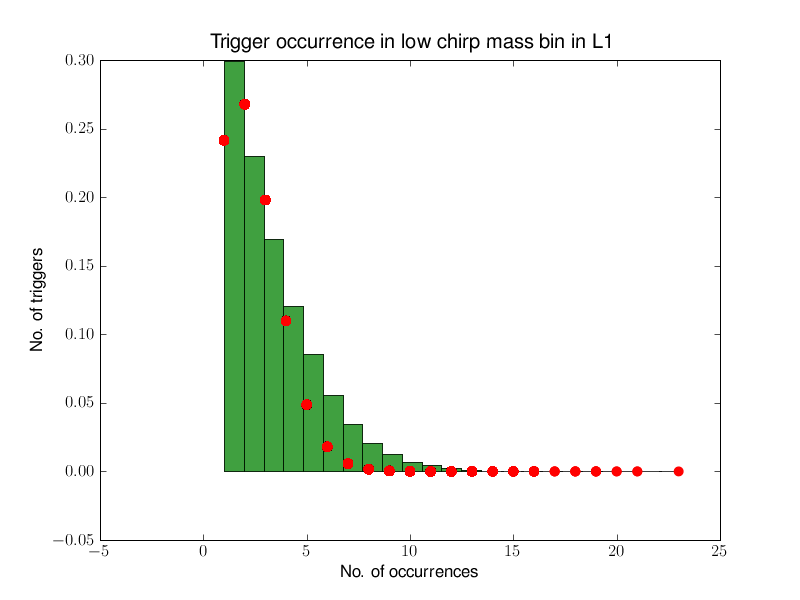
\includegraphics[scale=0.45]{Images/l1_low_distribution.png}
%\caption{Histogram of number of trigger occurrences in coincidences for GRB090809B: detector 1, low chirp mass bin (L1low)}
%\label{figure4}
%\end{minipage}
%\begin{minipage}[b]{0.5\linewidth}
\centering
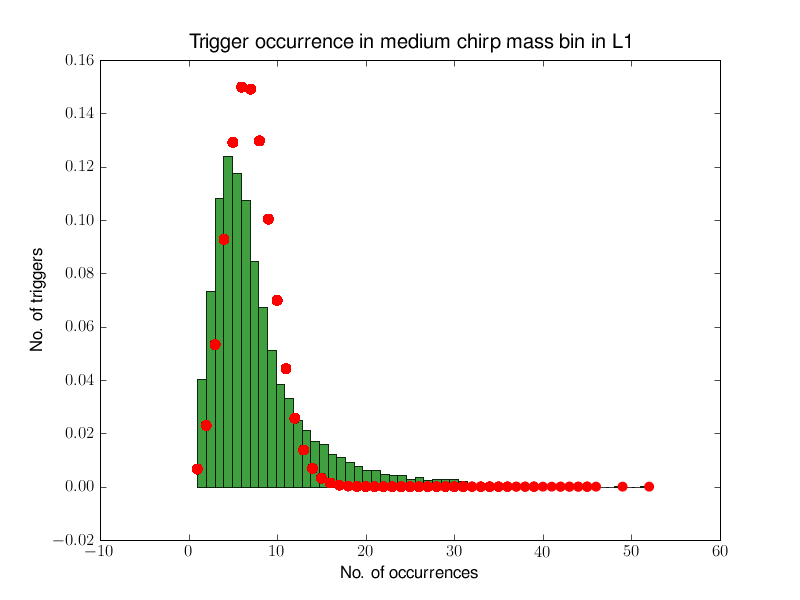
\includegraphics[scale=0.55]{Images/l1_medium_distribution.png}
%\caption{Histogram of number of trigger occurrences in coincidences for GRB090809B: detector 1, medium chirp mass bin (L1medium)}
%\label{figure5}
%\end{minipage}
%\begin{minipage}[b]{0.5\linewidth}
%\centering
%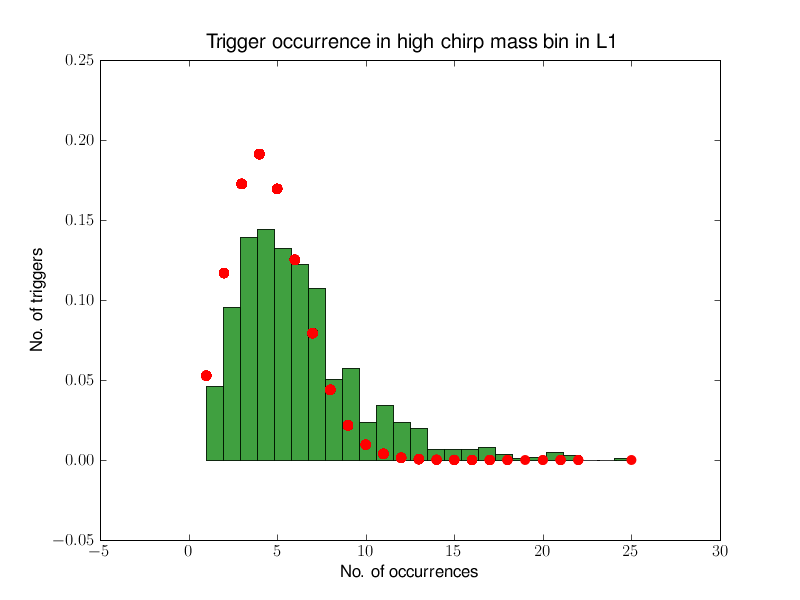
\includegraphics[scale=0.45]{Images/l1_high_distribution.png}
%\caption{Histogram of number of trigger occurrences in coincidences for GRB090809B: detector 1, high chirp mass bin (L1high)}
%\label{figure6}
%\end{minipage}
%\begin{minipage}[b]{0.5\linewidth}
%\centering
%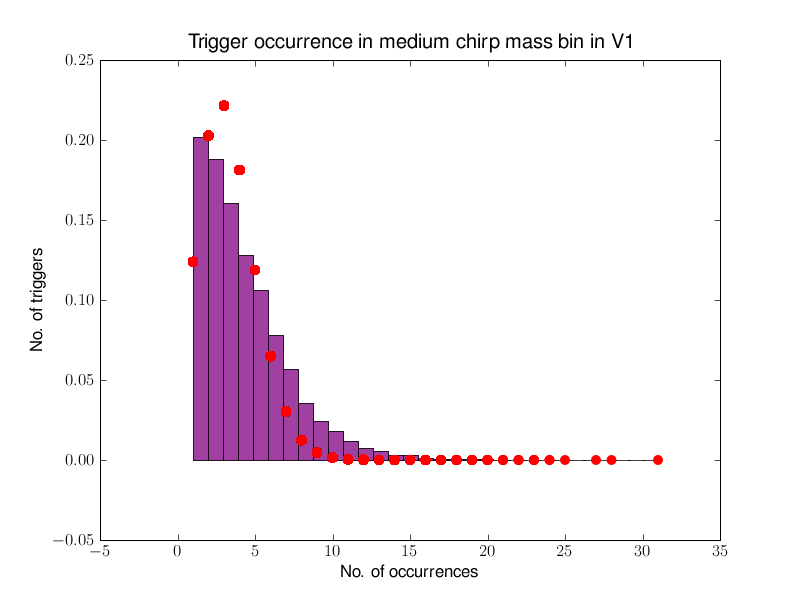
\includegraphics[scale=0.45]{Images/v1_medium_distribution.png}
%\caption{Histogram of number of trigger occurrences in coincidences for GRB090809B: detector 1, medium chirp mass bin (L1medium)}
%\label{figure5}
%\end{minipage}
\caption{Histogram of number of trigger occurrences in coincidences for a test GW--GRB coincident analysis with $S=160$ timeslides (for one of the detectors; normalization factor of 300 on the $y$--axis). Fitted (the dots) is the theoretical (expected) Poisson distribution of the number of occurrences, given by equation (\ref{poissontriggers}). The theoretical Poisson fit overestimates the number of triggers with low occurrence and underestimates the number of triggers with higher occurrence. This can be explained by correlations in trigger times due to non--Gaussian ``glitches''. We do not, however, notice a significant deviation from the predicted distribution; the expected occurrence for a fixed single detector trigger rate of 50 Hz, coincidence window width of $10^{-3}$ and 160 timeslides is $z=8$; the histogram peaks at roughly 5 occurrences.}
\label{poissonD}
\end{figure}

Figure \ref{poissonD} is a histogram of number of trigger occurrences in coincidences for a test GW--GRB coincident analysis with $S=160$ timeslides (for one of the detectors). Fitted (the dots) is the theoretical (expected) Poisson distribution of the number of occurrences, given by equation (\ref{poissontriggers}). The theoretical Poisson fit overestimates the number of triggers with low occurrence and underestimates the number of triggers with higher occurrence. This can be explained by correlations in trigger times due to non--Gaussian ``glitches''. Another explanation for these deviations is the choice of statistic for the model: a binomial distribution might be more suited to fit the histogram, since the Poisson distribution is an approximation of the binomial distribution. We do not, however, notice a significant deviation from the predicted distribution (whether it be Poisson or binomial); the expected occurrence for a fixed single detector trigger rate of 50 Hz, coincidence window width of $10^{-3}$ and 160 timeslides is $z=8$; the histogram peaks at roughly 5 occurrences. Since we would not have any reason to consider triggers be correlated, such a Poisson test--fit would be useful to identify the triggers that occur more than expected, thus finding correlations between triggers.

\subsection{Conclusions}
The chance that the distance to a short GRB is within the initial GW detector range is very low; we have used a very naive estimation of this chance probability and shown that it is of order $10^{-6} - 10^{-7}$. Given this, in order for a GW event, associated with a short GRB with no redshift measurement, to be considered a detection, its false alarm probability should be of order $10^{-6} - 10^{-7}$. We are unable to obtain such low FAP from the analysis of a single background GW data stretch for a GW--GRB analysis. Therefore we timeshift the data to create more coincident background. We have examined the simplest case of two coincident data stretches from two different GW detectors, with different trigger rates. We have estimated the size of a coincidence window and using this we have derived expressions for the background false alarm rate and its error, when timeshifting the data. Given a loud ``on--source'' event, the timeslides method may reduce the FAR error to a confidence interval that allows us to consider it a detection. The timeslides method is most efficient when working with detectors with similar trigger rate values. Imposing a higher SNR threshold will also add to this improvement by reducing the individual detector trigger rates and allowing for a larger number of timeslides to be performed. We have also shown that repeating single detector triggers in timeslid coincidences follow a distribution that resembles a Poisson distribution; such a distribution test may be used to identify non--Gaussian triggers that tend to show up in multiple coincidences across the timeslid background.

\section{Implementing timeslides in the analysis pipeline}

In the previous section we have shown theoretically that by performing timeslides we may be able to restrict the false alarm rate and probability to a confidence interval small enough to be comparable to an astrophysical probability that quantifies the chance a GRB was within the GW detectors' range. In the next section we will present how we implemented and tested the timeslides method in the case of an actual analysis.

\subsection{Test GRB}

The testing to implement timeslides in the coincident GRB analysis was done on an S6/VSR2 and 3 long GRB observed by Fermi--GBM, GRB090809B (trigger time GPS 933895709, date and time August 09 2009, 23:28:14 UTC, sky location RA=95.3, deg=0.1 degrees) \cite{gcn9760}. GRB090809B had available coincident data from Livingston L1 and Virgo V1. An inspection of the number of triggers participating in second--stage coincidences as function of SNR (Figure \ref{V1triggers}) reveals an exponential decrease with a long high--SNR tail and a high number of triggers near threshold ($\rho_0=4.5$); the high--SNR tail represents the population of ``glitches'' that reveal a non--Gaussian background.

\begin{figure}[ht]
\begin{minipage}[b]{0.5\linewidth}
\centering
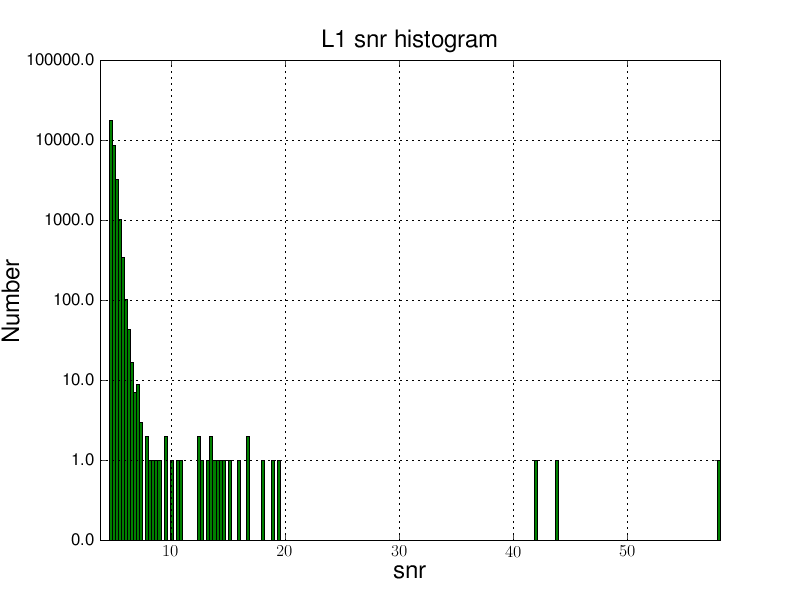
\includegraphics[scale=0.40]{Images/l1_triggers.png}
%\caption{Histogram of L1 triggers that participate in second--stage coincidences as function of SNR for GRB090809B. The majority of the triggers are at low SNR, near threshold; a tail of high--SNR ``glitches'' is present, revealing a non--Gaussian distribution of trigger events.}
%\label{L1triggers}
\end{minipage}
\hspace{0.5cm}
\begin{minipage}[b]{0.5\linewidth}
\centering
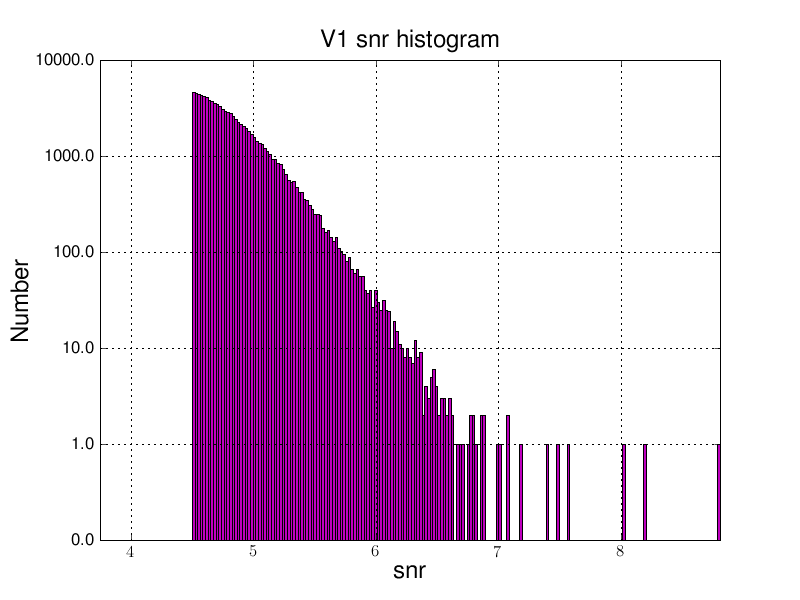
\includegraphics[scale=0.40]{Images/v1_triggers.png}
\end{minipage}
\caption{Left figure: histogram of L1 triggers that participate in second--stage coincidences as function of SNR for GRB090809B. The majority of the triggers are at low SNR, near threshold; a tail of high--SNR ``glitches'' is present, revealing a non--Gaussian distribution of trigger events. Right figure: histogram of V1 triggers that participate in second--stage coincidences as function of SNR for GRB090809B. The majority of the triggers are at low SNR but in this case the spread is more even across the SNR values with a much shorter tail of ``glitches''.}
\label{V1triggers}
%\end{minipage}
\end{figure}

\subsection{Implementation of timeslides}
The implementation of the timeslides analysis is fairly straightforward and uses the same basic principle as used in the previous all--sky searches \cite{Abbott:2009dk, Abadie:2010yba}. Given two arbitrary GW detectors $A$ and $B$, we can imagine the data from these detectors as rings and by fixing, say, detector $A$ data ring and rotating detector $B$ data ring by a certain \emph{slide amount}, a finite number of times, so that we will obtain new coincidence data. We keep rotating the detector $B$ ring until reaching the initial 0 position. In practice, this is done by translating in time--domain the data from one detector by a certain time amount $\Delta t$ with respect to the other (fixed in time) data from the other detector, making sure to re--attach the outstanding segment $\Delta t$ at the other end of the time--shifted detector data. By performing a finite $S$ number of such time--shifts of the data segments and repeating the coincidence tests described in Chapter \ref{Chapter Four} for every of the $S$ time--shifts, new coincidences are found and the background is sampled more finely as explained above.

Since for every timeslide $S$ we repeat the coincident stage of the pipeline, we will inherently obtain $S$ new lists of coincidences that should be clustered on trial and chirp mass in order to find the loudest coincident event in each of these trials, as explained in Chapter \ref{Chapter Four}, and masked for vetoing the trials that should be removed due to data quality reasons. The trial clustering and vetoes application is illustrated in Figure ~\ref{slidesGRB} and detailed below.

\begin{figure}[ht!]
\centering
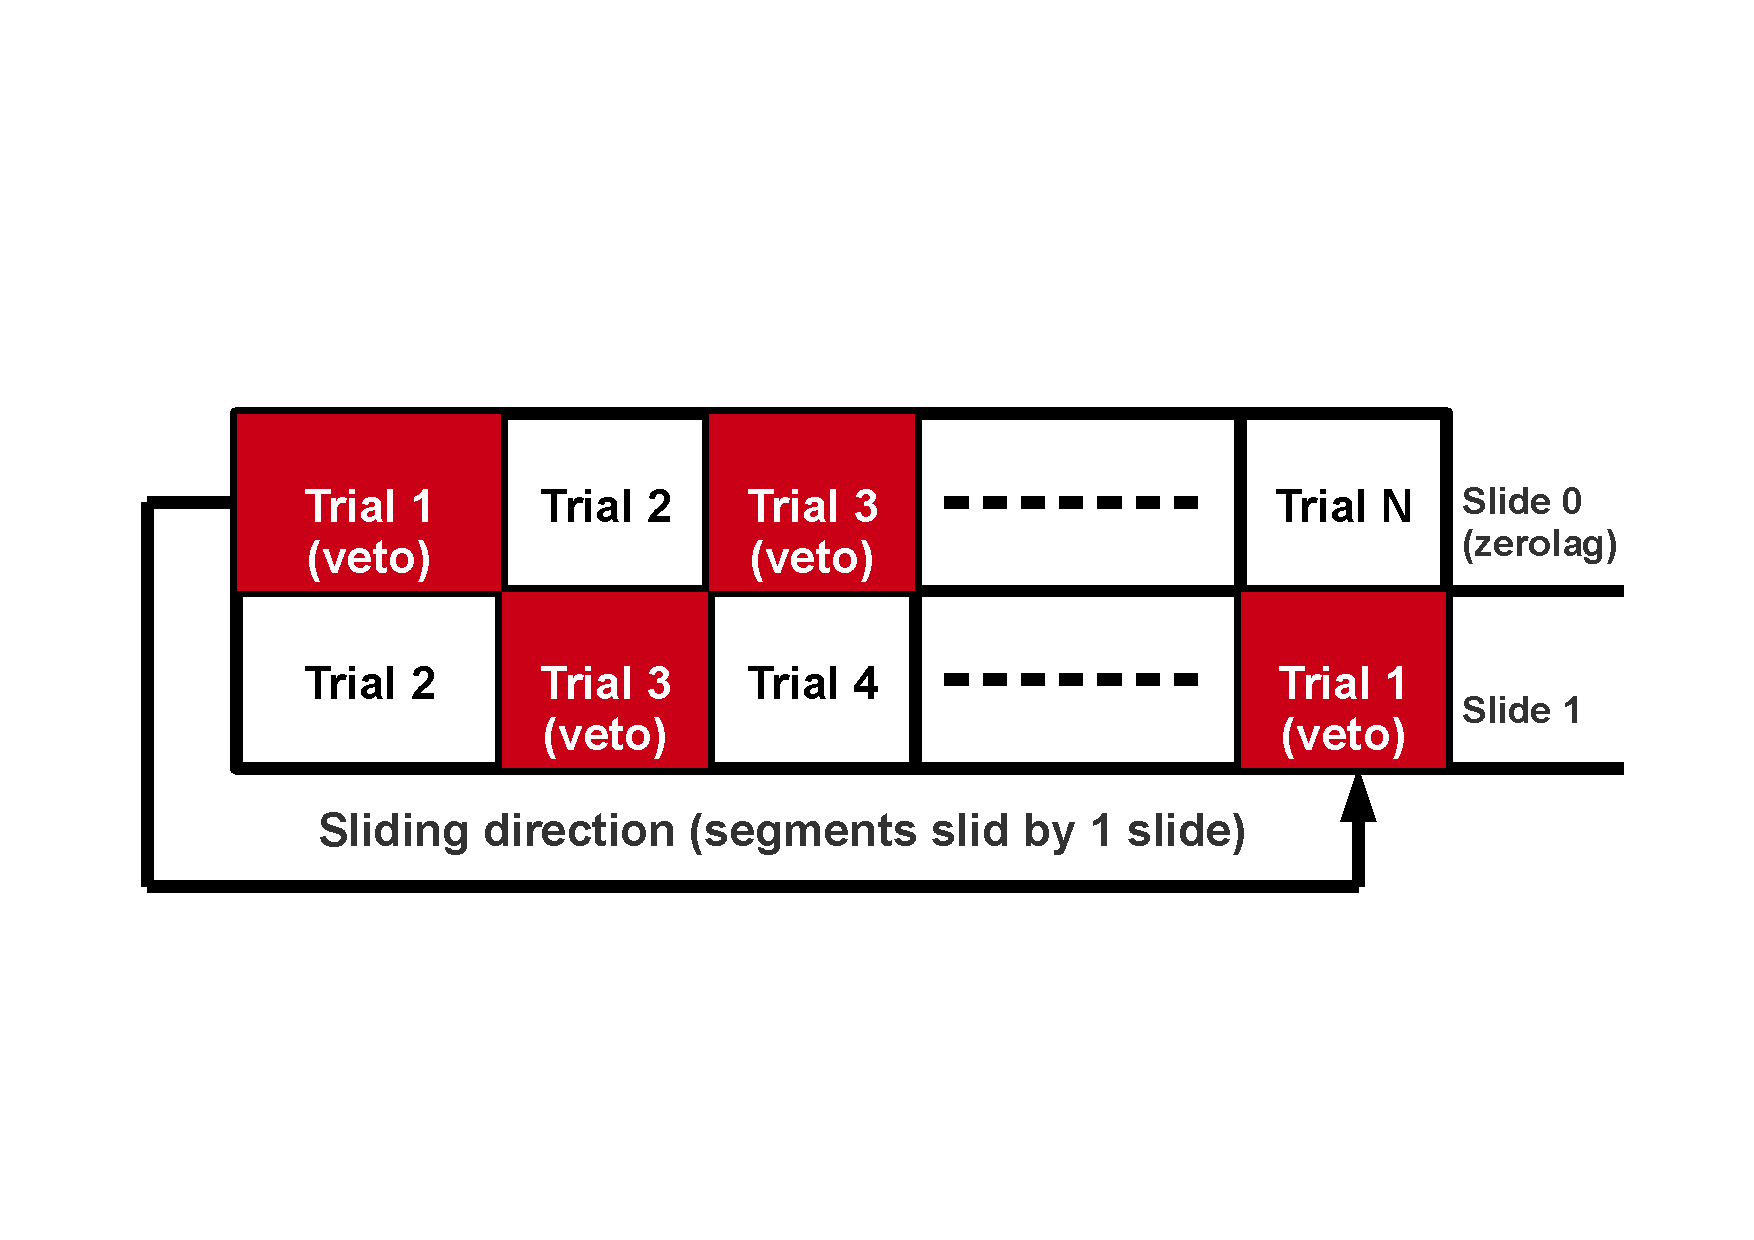
\includegraphics[scale=0.45]{Images/SlidingGRB.pdf}
\caption{Two--dimensional trial--slide veto mask designed to cluster coincidences in 6--s trials and apply vetoes in the case of a GRB analysis with timeslides: veto times (times of bad detector data) are overlapped with the ``zero--lag'' (Slide 0) that is partitioned in 6--s trials; the trials that fall during the veto times are marked as unwanted (full color here in the figure, example Trial 1) and none of the coincidences found in these trials will be considered for analysis. The first slide is built by timeshifting by a certain amount (usually multiples of 6--s, exactly 6--s in this figure, or the length of a trial) the whole ``zero--lag'' and re--attaching the remainder to the other end of the data stretch (Trial 1 here); the second slide is built in the same manner with reattaching the remainder (here it would be Trial 2) and so on. After $S$ timeshifts we will have a 2--dimensional (in trial along one dimension and slide number along the other) mask populated with valid and vetoed trials. We apply this mask to the actual time--shifted GW data and retain only the coincidences found in the un--vetoed trials.}
\label{slidesGRB}
\end{figure}

The coincident lists obtained from an analysis (matched--filtering, coincidence tests) with timeslides are stacked hierarchically starting from slide 0 (``zero--lag'') to slide $S$. At this stage we will partition each of these lists into 6--second trials, just as we would do in the case of a ``zero--lag'' analysis. We will want to discard the times of excessively noisy data by applying the data quality vetoes (as described in Chapter \ref{Chapter Four}, category two vetoes). The times to be vetoed are found in text lists parameterized by the start and end times of each of the bad data sectors. We overlap this list in time domain with the 0th slide (the ``zero--lag'') and mark each of the 6--s trials that fall during the vetoed times as unwanted; if a certain vetoed interval accounts for a non--integer number of 6--s trials, we discard all the trials that contain any veto times. This is done independently for every detector data. This will provide us with a 1--dimensional mask partitioned in 6--second trials that are either to contain coincident triggers to be taken account of in the analysis or to be discarded due to bad detector data. So far we have done this only for the 0th slide; sliding this mask with a certain slide amount for each timeslide will provide us with a two--dimensional trial--slide mask, populated with either empty timeshifted trials or with timeshifted veto trials. Coincidences falling in the vetoed trials are discarded, whereas those falling in a un--vetoed trial are kept.

\subsection{Test GRB results}
First, the background without timeslides (``zero--lag'') has been estimated and is shown in Figure \ref{datimeslides} (left). This is a cumulative histogram of background coincidences louder than a given SNR. Then the background obtained by doing $S=160$ timeslides has been estimated and is shown in Figure \ref{datimeslides} (right). The decrease in the FAP for background events is of order $\approx$160 (since we performed timeslides only for the off--source and we slid on two rings of 80 timeslides each), roughly the number of timeslides we performed.

\begin{figure}[ht!]
\begin{minipage}[b]{0.5\linewidth}
\centering
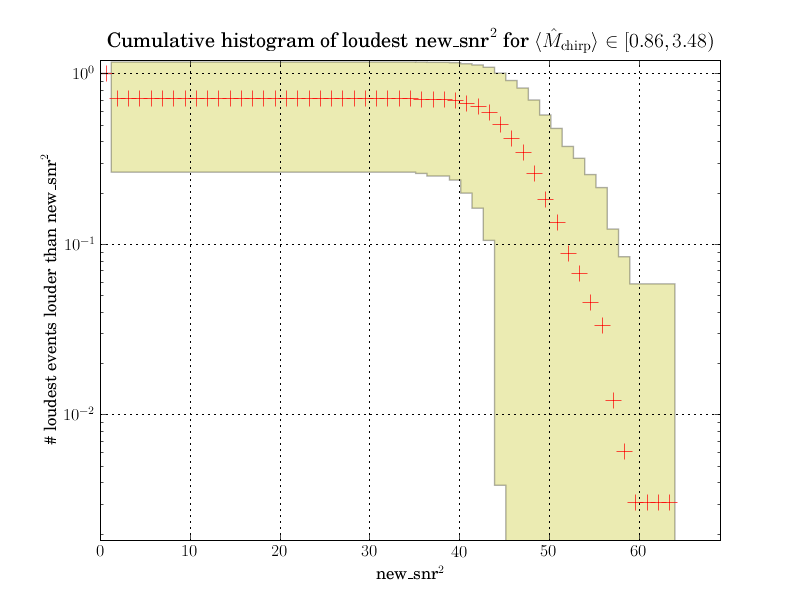
\includegraphics[scale=0.40]{Images/GRB090809B_lowmass_NOslides.png}
%\caption{Cumulative histogram of the loudest background events in the ``zero--lag'' case in the low chirp mass bin. The ``loudest'' events (highest effective SNR) populate the tail of the distribution at FAP of order 1/300.}
%\label{niettimeslides}
\end{minipage}
\hspace{0.5cm}
\begin{minipage}[b]{0.5\linewidth}
\centering
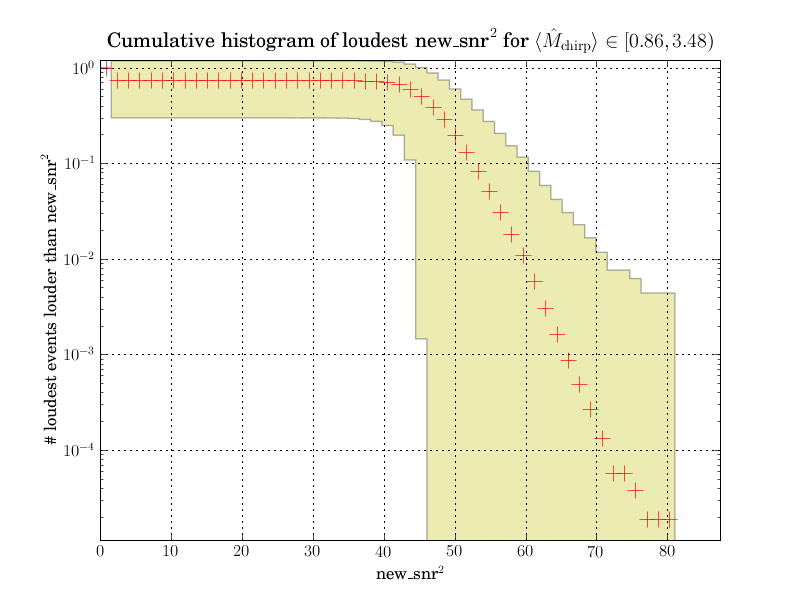
\includegraphics[scale=0.40]{Images/GRB090809B_lowmass_80slides.png}
\end{minipage}
\caption{Cumulative histogram of the loudest background events: left figure in the ``zero--lag'' case in the low chirp mass bin -- the ``loudest'' events (highest effective SNR) populate the tail of the distribution at FAP of order 1/300; right figure in the timeslides (160 timeslides) case in the low chirp mass bin -- the ``loudest'' events (highest effective SNR) populate the tail of the distribution at FAP of order 1/$300 \times 160$$\approx 2 \times 10^{-5}$.}
\label{datimeslides}
%\end{minipage}
\end{figure}

Estimating the background using timeslides does not change the overall average background distribution since most of the coincidences are consisted of low--SNR triggers that will produce more and more low--SNR coincidences once timeslides are performed. Timeslides add to the loud--SNR tail though; the larger the number of timeslides is the larger the chances to have loud events in the tail, louder than the ``zero--lag'' loudest triggers, as shown in Figures \ref{090809B_onsource_slides} (left) and \ref{090809B_onsource_slides} (right). 

\begin{figure}[ht!]
\begin{minipage}[b]{0.5\linewidth}
%\centering
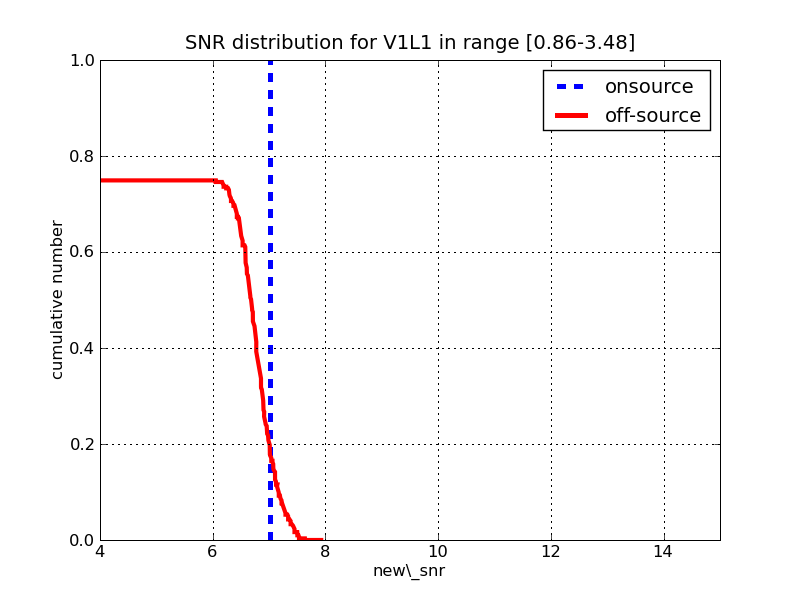
\includegraphics[scale=0.40]{Images/090809B_onsource_noslides.png}
%\caption{Background distribution (continuous line) and loudest on--source event (dashed line) when no timeslides are performed (``zero--lag'').}
%\label{090809B_onsource_noslides}
\end{minipage}
%\hspace{0.5cm}
\begin{minipage}[b]{0.5\linewidth}
%\centering
\includegraphics[scale=0.40]{Images/090809B_onsource_slides.png}
%\label{090809B_onsource_slides}
\end{minipage}
\caption{Background distribution (continuous line) and loudest on--source event (dashed line): left figure when no timeslides are performed (``zero--lag''); right figure when 160 timeslides are performed. The timeslides produce events louder that the ``zero--lag'' loudest events.}
\label{090809B_onsource_slides}
%\end{minipage}
\end{figure}

\subsection{Timeslides in the coherent search}

The work in the coincident pipeline is finished; since we are using the coherent pipeline for GRB analyses, we have started the work to implement timeslides in this pipeline as well. The coherent pipeline splits the time series data in segments 128 s long. Long timeslides are just a reshuffling (renaming) of these segments and are done before the FFT and match filtering stages. One may choose to do as many timeslides as desired, they are circular, but there is no point in doing more timeslides than the total number of segments since they repeat themselves (circularily symmetric). Long timeslides are labeled ``long'' since we shift the whole data by a certain amount and not each segment internally, which would be called short timeslides. Long timeslides have already been implemented in the search codes, but the work on postprocessing, involving data quality veto handling, is still to be completed at the time of this writing.

\section{Restriction on inclination angle for nearly face--on binaries}

It is very important to use results of astrophysical observations in GW searches. This is motivated twofold: first, especially in the case of triggered modelled searches, because we want to characterize our target source as accurately as possible. Astrophysically--motivated priors will improve GW detection chances and allow for accurate recovery of parameters. Second, because by using certain astrophysical priors one may reduce the search parameter space and speed up the analysis. 

One such proposed prior would be to limit the inclination angle $\iota$ in the case of a \ac{GW} search triggered by a short GRB. There are two assumptions that lead to a restriction on inclination angle: the jet opening angle from a short burst is small and the \ac{GW} from a short GRB are emitted along the axis of total angular momentum. The first assumption, as we have seen in Chapter \ref{Chapter Two}, is supported by a number of implicit argumets that assume similarity between other high--energy sources that are collimated (AGN, micro--quasars) and short gamma--ray bursts; also, the GRB energetics can be explained by a jet--like emission. There is only one direct astrophysical observation of the jet break for a short burst -- GRB051221A \cite{Burrows:2006ar}, estimating a half--opening angle of 4--8 degrees, but it is believed, analogous to long soft GRBs, that the emission is collimated for short GRBs as well.

We will present a framework allowing us to implement an astrophysical prior on inclination in the case of the coherent analysis pipeline (see Chapter \ref{Chapter Three} for data analysis theory and Chapter \ref{Chapter Four} for pipeline description).

\subsection{Theoretical considerations}

We will consider two separate cases for a short gamma-ray burst produced by a compact binary merger: the binary orbit is ``face--on'' with respect to the GW detectors' plane, i.e., the inclination angle $\iota$ is close to 0 and the binary orbit is ``face--away'' with respect to the GW detectors' plane, i.e., the inclination angle $\iota$ is close to $\pi$. These approximations will be used in computing the amplitude terms $\mathcal{A}^{\mu}$ (see Chapter \ref{Chapter Three} for definitions of amplitude terms) by Taylor--expanding $\cos \iota$ around 0 and $\pi$ keeping only the first leading order terms. The approximation stands well up to angles of order 40 degrees, see Figure \ref{cos_and_approximant}; this is a good indicator that we are not restricting the inclination (and consequently the jet--opening angle) in a too strict of a manner, given that the astrophysical data is not conclusive in the case of short hard GRBs.

\begin{figure}[ht!]
\centering
\includegraphics[scale=0.55]{Images/cos_and_approximant.png}
\caption{$\cos \iota$ (continous line) its second--order approximation $1- \frac {{\iota}^2}{2}$ obtained by Taylor--expanding it around 0 (dashed line) and $\frac {1+\cos^2 \iota}{2}$ (dash--dot line). The function and its approximants are almost identical up to high values ($\approx$40 degrees). The same behavior can be seen by Taylor--expanding $\cos \iota$ around $\pi$, with a sign reversion.}
\label{cos_and_approximant}
\end{figure}

\subsubsection{Approximate case $\iota \rightarrow 0$}

Taylor expansion of $\cos \iota$ around 0:
%
\begin{equation}
\cos \iota (\iota \rightarrow 0) = 1- \frac {{\iota}^2}{2}+\frac {{\iota}^4}{4!}+\mathcal{O}({\iota}) \approx 1- \frac {{\iota}^2}{2}
\end{equation}
%
With this in mind we obtain an approximate expression for $\frac {1+\cos^2 \iota}{2}$, expanding again $\cos \iota$ in power series:
%
\begin{equation}
\frac {1+\cos^2 \iota}{2} \approx \frac{1+(1- \iota^2/2! + \iota^4/4!)^2}{2} \approx 1- \frac {{\iota}^2}{2} + \frac {{\iota}^4}{24}\approx 1- \frac {{\iota}^2}{2} \approx \cos \iota,~\iota \rightarrow 0 
\end{equation}
%
We will follow the derivation steps presented in detail in \cite{Harry:2010fr} and summarized in Chapter \ref{Chapter Three}. The waveform amplitudes $\mathcal{A}^{\mu}$, using the expansion of $\cos \iota$, will reduce to:
%
\begin{equation}
\label{eqn:a1}
\mathcal{A}^1 \approx - \frac{D_0}{D} \cos \iota \cos(2(\phi_0-\psi))= - \frac{D_0}{\tilde{D}} \cos (2 \chi_-)
\end{equation}
\begin{equation}
\label{eqn:a2}
\mathcal{A}^2 \approx \frac{D_0}{D} \cos \iota \sin(2(\phi_0-\psi))= \frac{D_0}{\tilde{D}} \sin (2 \chi_-)
\end{equation}
\begin{equation}
\label{eqn:a3}
\mathcal{A}^3 \approx - \frac{D_0}{D} \cos \iota \sin(2(\phi_0-\psi))= - \frac{D_0}{\tilde{D}} \sin (2 \chi_-)
\end{equation}
\begin{equation}
\label{eqn:a4}
\mathcal{A}^4 \approx - \frac{D_0}{D} \cos \iota \cos(2(\phi_0-\psi))= - \frac{D_0}{\tilde{D}} \cos (2 \chi_-)
\end{equation}
%
where $\tilde{D} = D/\cos \iota$ is an effective distance and $\chi_- = \phi_0-\psi$ is an effective phase angle. Therefore, the amplitudes are now function of only two variables, $\tilde{D}$ and $\chi_-$.

Introducing the antenna factors $\mathrm{F}_+=\mathrm{F}_+(\theta, \varphi)$ and $\mathrm{F}_{\times}=\mathrm{F}_{\times}(\theta, \varphi)$ we write the waveform at the detector as $\mathrm{h(t)}= \mathrm{F}_+(\theta, \varphi)\mathrm{h_+(t)}+\mathrm{F}_{\times}(\theta, \varphi)\mathrm{h_{\times}(t)}$ and replacing the amplitude expressions ~(\ref{eqn:a1},~\ref{eqn:a2},~\ref{eqn:a3},~\ref{eqn:a4}) in equation (\ref{eq:h_plus_cross}) we obtain the waveform as a linear combination of the orthogonal complex components $h_0(t)$ and $h_{\pi/2}(t)$. The two polarizations of the gravitational waveform will then be:
%
\begin{eqnarray}
h_+(t) = -\frac{D_0}{\tilde{D}} \cos(2\chi_-) h_0(t) -\frac{D_0}{\tilde{D}} \sin(2\chi_-) h_{\pi/2}(t) \nonumber \\
h_{\times}(t) = \frac{D_0}{\tilde{D}} \sin(2\chi_-) h_0(t) -\frac{D_0}{\tilde{D}} \cos(2\chi_-) h_{\pi/2}(t)
\end{eqnarray}
%
This way the waveforms will depend on only two amplitudes $B_1$ and $B_2$, as opposed to having the four amplitudes from equation (\ref{eq:amplitude_def}):
% 
\begin{eqnarray}
B_1=\frac{D_0}{\tilde{D}}\cos(2\chi_-)=-A^1=-A^4 \nonumber \\
B_2=\frac{D_0}{\tilde{D}}\sin(2\chi_-)=A^2=-A^3
\end{eqnarray}
%
With these, we can express the two gravitational waveform polarizations as
%
\begin{eqnarray}
h_+=-B_1h_0-B_2h_{\pi/2} \nonumber \\
h_{\times}=B_2h_0-B_1h_{\pi/2}
\end{eqnarray}
%
Since CBC signals will spend a large number of cycles in the sensitive band of the detector, the 0 and $\pi/2$ phases will be close to orthogonal, i.e., $(h_0|h_{\pi/2}) \approx 0$ and $(h_0|h_0) \approx (h_{\pi/2}|h_{\pi/2}) = \sigma^2$. We can write the multi--detector log--likelihood expressed by equation (\ref{eq:multi_log_lambda}):
%
\begin{eqnarray}
\mathrm{ln}\Lambda &=& ({\bf s}|{\bf h})- \frac{1}{2}({\bf h}|{\bf h}) \nonumber \\
                   &=& A^{\mu}({\bf s}|h_{\mu}) - \frac{1}{2}A^{\mu}M_{\mu \nu}A^{\nu}
\end{eqnarray}
%
where, $h_{\mu} = (h_1,h_2,h_3,h_4) = (F_+h_0,F_{\times}h_0,F_+h_{\pi/2},F_{\times}h_{\pi/2})$ and, if working in the dominant polarization approximation, $M_{\mu \nu}$ is a diagonal matrix expressed as $M_{\mu \nu}=\mathrm{diag}(\sigma^2F_+^2, \sigma^2F_{\times}^2, \sigma^2F_+^2, \sigma^2F_{\times}^2)$. We will assume summation over the $k$ detectors, but we will write the explicit sum terms only for the final expression, for ease of notation. We wish to express the multi--detector likelihood as function of $B_1$ and $B_2$ only:
%
\begin{eqnarray}
\mathrm{ln}\Lambda &=&-B_1\left((s|F_+h_0)+(s|F_{\times}h_{\pi/2})\right)+B_2\left((s|F_{\times}h_0)-(s|F_+h_{\pi/2})\right) \nonumber \\
        &&-\frac{1}{2}\left(B^2_1+B^2_2\right)(\sigma^2F_+^2+\sigma^2F_{\times}^2)
\label{liken}
\end{eqnarray}
%
Maximizing the likelihood $\Lambda$ function over the two amplitude parameters $B_1$ and $B_2$, gives us the amplitudes values:
%
\begin{eqnarray}
B_1=\frac{(s|F_+h_0)+(s|F_{\times}h_{\pi/2})}{\sigma^2F_+^2+\sigma^2F_{\times}^2}~~\mathrm{and} \nonumber \\
B_2=-\frac{(s|F_{\times}h_0)-(s|F_+h_{\pi/2})}{\sigma^2F_+^2+\sigma^2F_{\times}^2}
\end{eqnarray}
%
and replacing these expressions in the likelihood (\ref{liken}) and introducing summation over the $k$ number of detectors:
%
\begin{eqnarray}
\rho^2&:=&2\mathrm{ln}\Lambda|_{\mathrm{max}} \nonumber \\ 
       &=& \frac{\left(\sum_k(s^k|F_+^kh_0^k)+\sum_k(s^k|F_{\times}^kh_{\pi/2}^k)\right)^2+\left(\sum_k(s^k|F_{\times}^kh_0^k)-\sum_k(s^k|F_+^kh_{\pi/2}^k)\right)^2}{\sum_k\left(F_+^{k,2}+F_{\times}^{k,2}\right)(h_0^k|h_0^k)} \nonumber \\
       &&
\end{eqnarray}
%
it is easy to see that the SNR is now $\chi^2$ distributed with two degrees of freedom.

\subsubsection{Approximate case $\iota \rightarrow \pi$}
Following the same steps as above, Taylor--expanding $\cos \iota$ around $\pi$ this time and replacing in the new values:
%
\begin{equation}
\cos \iota (\iota \rightarrow \pi) = -1+ \frac {{\iota}^2}{2}+\mathcal{O}({\iota}^4) \approx -1+ \frac {{\iota}^2}{2}
\end{equation}
%
and 
%
\begin{equation}
\frac {1+\cos^2 \iota}{2} \approx -\cos \iota,\iota \rightarrow \pi 
\end{equation}
In this case, as above, the expressions for the approximate amplitudes will be:
%
\begin{equation}
\label{eqn:a12}
A_1 \approx - \frac{D_0}{D} \cos \iota \cos(2(\phi_0+\Psi))= - \frac{D_0}{\tilde{D}} \cos (2 \chi_+)
\end{equation}
\begin{equation}
\label{eqn:a22}
A_2 \approx \frac{D_0}{D} \cos \iota \sin(2(\phi_0+\Psi))= \frac{D_0}{\tilde{D}} \sin (2 \chi_+)
\end{equation}
\begin{equation}
\label{eqn:a32}
A_3 \approx - \frac{D_0}{D} \cos \iota \sin(2(\phi_0+\Psi))= - \frac{D_0}{\tilde{D}} \sin (2 \chi_+)
\end{equation}
\begin{equation}
\label{eqn:a42}
A_4 \approx - \frac{D_0}{D} \cos \iota \cos(2(\phi_0+\Psi))= - \frac{D_0}{\tilde{D}} \cos (2 \chi_+)
\end{equation}
%
where, again, $\tilde{D} = D/\cos \iota$ is an effective distance and $\chi_+ = \phi_0+\psi$ is an effective phase angle. Therefore, the amplitudes are again function of only two variables, $\tilde{D}$ and $\chi_+$. In a similar manner, the two GW polarizations are:
%
\begin{eqnarray}
h_+(t) = \frac{D_0}{\tilde{D}} \cos(2\chi_+) h_0(t) +\frac{D_0}{\tilde{D}} \sin(2\chi_+) h_{\pi/2}(t) \nonumber \\
h_{\times}(t) = \frac{D_0}{\tilde{D}} \sin(2\chi_+) h_0(t) -\frac{D_0}{\tilde{D}} \cos(2\chi_+) h_{\pi/2}(t)
\end{eqnarray}

Using the same reduced amplitude terms $B_1$ and $B_2$, the polarizations simplify to
%
\begin{eqnarray}
h_+=B_1h_0+B_2h_{\pi/2} \nonumber \\
h_{\times}=B_2h_0-B_1h_{\pi/2}
\end{eqnarray}
%
We will use the same derivation steps for the multi--detector likelihood as in the case $\iota \rightarrow 0$, maximizing over the amplitude terms$B_1$ and $B_2$, and replacing the amplitude expressions in the likelihood, we obtain:
%
\begin{eqnarray}
\rho^2&:=&2\mathrm{ln}\Lambda|_{\mathrm{max}} \nonumber \\ 
       &=& \frac{\left(\sum_k(s^k|F_+^kh_0^k)-\sum_k(s^k|F_{\times}^kh_{\pi/2}^k)\right)^2+\left(\sum_k(s^k|F_{\times}^kh_0^k)+\sum_k(s^k|F_+^kh_{\pi/2}^k)\right)^2}{\sum_k\left(F_+^{k,2}+F_{\times}^{k,2}\right)(h_0^k|h_0^k)} \nonumber \\
       &&
\end{eqnarray}
%
it is easy to see that the SNR is again $\chi^2$ distributed with two degrees of freedom.

The new detection statistic will be distributed as two $\chi^2$ distributions with 2 degrees of freedom each, each for the $\iota \rightarrow 0$ and $\iota \rightarrow \pi$ cases. We wish to compare this statistic to the standard coherent SNR that is $\chi^2$--distributed with 4 degrees of freedom, given by equation (\ref{eq:fstat_plus_cross}) (see Chapter \ref{Chapter Three}). The difference between two $\chi^2$ distributions with 2 degrees of freedom each and one with 4 degrees of freedom can be seen in Figure \ref{chi_2_and_4}. We notice a decrease of FAP at fixed SNR of roughly one order of magnitude and an increase in sensitivity at fixed FAP of roughly 5\%. The increase in sensitivity could be larger in real noise since glitches tend to give high SNR in only one detector, hence best matched by an edge--on case; this could prove efficient as a glitch--rejection mechanism.

\begin{figure}[ht!]
\centering
\includegraphics[scale=0.60]{Images/chi_sq_2_and_4.png}
\caption{Difference between two $\chi^2$ distributions with 2 degrees of freedom (DOF) each (dashed red line) and one with 4 DOF (blue continuous line) -- semilog--$y$; the $\rho^2$ represents the network SNR. Imposing a $\iota \rightarrow 0$ or $\iota \rightarrow \pi$ condition in the analysis, generates an SNR that is two $\chi^2$ ,2 DOF each, distributed, whereas the standard coherent SNR is $\chi^2$ ,4 DOF, distributed. We notice a decrease of FAP at fixed SNR of roughly one order of magnitude and an increase in sensitivity at fixed FAP of roughly 5\%.}
\label{chi_2_and_4}
\end{figure}

\section{Discussion}

In this chapter we have introduced a number of developments to the existing templated triggered searches associated with short GRBs. We have estimated, in a very naive way, the probability of a GRB to occur within the detection range of the present LIGO and Virgo. This probability should be comparable to the false alarm probability of any given ``on--source'' event in order for us to attempt at a detection claim. The very low value of this astrophysically motivated probability prompted us to investigate methods that lead to a better estimation of the GW background. We have introduced and presented the theoretical framework and implementation of a method that estimates the background for a coincident triggered GW--GRB search using timeslides. This method uses unphysical time segments that are produced by time--sliding physical data segments from different GW detectors. The main advantage of such a method is that it reduces the error of the background false alarm rate; this method proves most efficient in the case of data from GW detectors with low and similar trigger rates. The implementation of timeslides in the CBC code is relatively straightforward and uses much of the already present infrastructure; the main challenge in implementing it was handling the data quality vetoes.

Based on the assumption that short GRB are highly beamed, we have presented the theoretical framework for a method that restricts the binary inclination angle $\iota$ to 0 or $\pi$, when performing a GW--GRB analysis. This method is still to be tested and implemented, but the theoretical predictions show an increase in search sensitivity of $\sim$5\% at a fixed FAP or a decrease in FAP of one order of magnitude at fixed SNR, compared to a search that draws $\iota$ values uniformly between 0 and $\pi$. This would prove to be a strong ``glitch''--rejection mechanism as well, given that non--Gaussian triggers will have recovered inclination angles randomly distributed between 0 and $\pi$. In terms of errors, a variation $\delta \iota \ll \iota$ would introduce an error term of order $\iota \delta \iota \ll 1$ to first order approximation. The implementation of this restrictive method will be using a relatively large window for the inclination angle, so that to account for wider--jet scenarios, but small enough for the approximations to hold. 



\chapter{Search for gravitational waves associated with the InterPlanetary Network gamma-ray bursts -- Methodology} % Write in your own chapter title
\label{Chapter Six}
%\lhead{Chapter~\ref{ChapterLabel}
% \emph{Search for Gravitational Waves Associated with the InterPlanetary Network Gamma--Ray Bursts -- Methodology}} % Write in your own chapter title to set the page header

This chapter reports the motivation and methodology for a search in GW data around the times of 20 additional gamma-ray bursts during S5/VSR1. These bursts were detected between 2006 and 2007 and have been localized, in both time and sky location, such that a targeted GW search is possible. I will discuss the necessary changes to the recently finished analysis (for the S6/VSR2 and 3 science runs \emph{Swift} and Fermi--GBM--observed GRBs, \cite{lvc:s6grb, Harry:2010fr}, and Chapter \ref{Chapter Four} for an example analysis) that are needed to implement a search on GRBs identified by the IPN network which may be less well localized in both sky position and time than the corresponding bursts identified by the Swift satellite and used in previous analyses \cite{Abadie:2010uf, Collaboration:2009kk}.

We gathered the sample of GRBs to be analyzed using data provided in the IPN online table available publicly at \cite{HurleyHTML} and by cross-checking this with NASA's HEASARC online table at \cite{heasarc}. Since these GRBs are not reported in any of NASA's Gamma Ray Burst Circulars (GCN) \cite{gcns}, a manual check on each burst had to be performed in order to confirm its characteristics, involving checking several IPN satellite homepages e.g., Suzaku at \cite{suzaku}, INTEGRAL at \cite{integral}, \emph{Swift} at \cite{swift} and Konus--WIND at \cite{konus}.

The details of the sky position were obtained by manually processing raw data from the IPN satellites for every GRB.  In order to perform a search of the GW data for a given GRB, the sky position and time of the GRB must be determined.  This information is obtained from knowledge of: the IPN satellites that detected the burst together with their absolute and relative sky positions (information needed for constructing the GRB error boxes), locations of all the spacecraft (used to obtain the blocking constraints to reduce the size of the GRB error boxes), the burst time of arrival at the satellites and at Earth (used to determine the time interval on which we will perform the GW search) and its error. Constructing the GRB error boxes, determining their sizes and choosing the right GW data for analysis are entirely contingent on these pieces of information.

\begin{figure}[htb]
\begin{center}
\includegraphics[height=15pc]{Images/ipn1.pdf}
\caption{\label{fig:triangulation}The IPN schematics: triangulating the position of a GRB using three IPN spacecraft (S1, S2 and S3). Using three satellites we obtain two IPN annuli that intersect to form two error boxes. Reference \cite{HurleyHTML}}
\end{center}
\label{IPNtriangulation}
\end{figure}

\section{The IPN triangulation mechanism}
The InterPlanetary Network \cite{Hurley:2002wv, Hurley:1999ym}, also summarized in Chapter \ref{Chapter Two}, employs several space missions and synthesizes data obtained from the detection of the same burst by different spacecraft equipped with gamma-ray detectors. The IPN has been operating for three successive generations; presently the third IPN (IPN3) began its operation in November 1990. Currently the spacecraft gathering data are Konus-WIND, Suzaku, INTEGRAL,  RHESSI, \emph{Swift}, Fermi--GBM (in Earth orbit), MESSENGER (in Mercury orbit) and Mars Odyssey (in Mars orbit) \cite{HurleyHTML}. When the duty cycles and effective fields of view of all the missions in the network are considered, the IPN is an all--time, isotropic GRB monitor.

The principle on which the IPN triangulation method is based uses the arrival time of the same burst at different spacecraft to determine the source sky location. Figure \ref{fig:triangulation} illustrates how an IPN triangulation works. S1, S2 and S3 denote three spacecraft detecting the same GRB and $\theta$ is angle between the burst direction and the baseline between S1 and S2.  Then, the burst will be detected by S2 at a time $\delta T$ seconds earlier than S1 
%
\begin{equation}
\cos (\theta) = c \delta T / D_{12}
\label{IPNeqn1}
\end{equation}
%
where $D_{12}$ is the distance between S1 and S2, and $c$ the speed of light. Since $D_{12}$ is known and $\delta T$ is measured, $\theta$ is estimated. The solution to equation (\ref{IPNeqn1}) is represented by a ring, or an $annulus$, whose width depends on the timing uncertainties ($\sigma(\delta T)$) and on the separation $D_{12}$.  The further apart the detectors, the more precise the localization. The number of independent couples of detectors (and, therefore, the number of independent annuli) is two for the case of three spacecraft; thus, the burst direction must be inside one of the two intersection regions of the annuli. This intersection region is called the IPN error box of the GRB. Depending on the location of the IPN spacecraft and their timing errors this error box may vary in size from fractions of, to hundreds of square degrees. The annulus width is obtained by propagating the uncertainty on the time delay $\delta T$. Thus, from equation (\ref{IPNeqn1}) it follows that
%
\begin{equation}
\sigma(\theta) = \frac{c\sigma (\delta T)}{D_{12} \sin (\theta)}
\label{IPNeqn2}
\end{equation}

Equation (\ref{IPNeqn2}) gives the uncertainty $\sigma(\theta)$ in the angle $\theta$ expressed in radians.  The uncertainty on $D_{12}$ has been neglected, as the main contribution comes from the timing uncertainties. One has to take into account not only the time resolution of each of the detectors, but also the difficulty of comparing different light curves, often derived from different energy bands. For example, when $D_{12}$ spans the typical range: few $10^2$ - few $10^3$ light seconds, then from equation (\ref{IPNeqn2}) it comes out that a minimum time resolution of the order of $10^{-2} - 10^{-3}$ s is required, in order to have $\sigma(\theta) \sim$ few arcminutes or less in order to obtain a precise localization.

\begin{figure}[htb]
\begin{center}
\includegraphics[width=32pc]{Images/Slide1.png}
\caption{\label{fig:error_box}Error box construction: red lines correspond to the Konus-WIND ecliptic latitude bands, blue lines are the 3--$\sigma$ IPN1-2 annulus and magenta lines are the 3-$\sigma$ IPN1-3 annulus obtained by triangulation (in this case we have three IPN spacecraft observing the same burst). The error boxes are the solid regions bounded by the intersections of the IPN annuli and ecliptic bands. }
\end{center}
\label{errorbox}
\end{figure}

\section{The IPN GRB error box construction}

The error boxes for the IPN GRBs are constructed from the intersection of the triangulated 3-$\sigma$ IPN annuli and different field--of--view blocking constraints (if present). See Figure \ref{fig:error_box} for an illustration example. When the constraints involve Konus-WIND ecliptic latitude bands, the error box that will be kept is located between the ecliptic bands. The reason for this is that the Konus-WIND spacecraft consists of two detectors, one facing the north ecliptic pole, and the other facing the south ecliptic pole. By comparing the count rates on these two detectors, the Konus team obtains an estimate of the ecliptic latitude of the burst. Typically, the band is 20-30 degrees wide, and it is good to a 90--95\% confidence; systematic and statistical errors usually prevent it from being much more accurate than this value. In those cases where we have a single triangulation annulus, plus an ecliptic latitude band, the result is often two long, narrow error boxes, where the annulus intersects the band. Konus-WIND is positioned at a Lagrange point between Earth and Sun (L1) and it has two GRB detectors - Konus1 that points southward and Konus2 that points northward. By comparing the event count rates from the two detectors one can provide a spacecraft spin elevation measurement that translates to an ecliptic latitude source location. This is always at the same sky location (since Konus is fixed with respect to Earth--Sun, RA $\sim 270^{\circ}$, dec $\sim 66^{\circ}$) with a constant difference in radii (width) of about $20-30^{\circ}$. Konus provides active location of IPN GRBs twofold: by introducing this ecliptic band (which is independent of triangulation with other spacecraft) that superimposed with other IPN annuli reduces the overall area of the error boxes \emph{and} contributes to the timing and triangulation of IPN annuli together with other IPN spacecraft.Other intersections are possible, too, such as a single long, narrow error box if the IPN annulus grazes the ecliptic latitude band. Also, anything that overlaps a region where a planet blocks the view will be discarded.

\section{Determining the GRB time of arrival}

The Earth crossing time, also referred to as the time of arrival of the burst, is the time when the gamma ray signal would cross the center of the Earth and is the reference time to be considered when constructing the time search window for gravitational waves. 
This time can only be estimated based on the burst arrival times at the different IPN satellites and based on their positions with respect to Earth. This way of choosing the burst time is prone to two types of uncertainties: the first is simply the fact that we may not have the time at Earth but at a satellite that is separated from Earth by a certain distance; the error is directly proportional to the distance to Earth where the closest IPN satellite is located at the time of the burst. The best estimate comes from any satellite that is not interplanetary (i.e. not on orbit around Mars or at a distant point from Earth).  These ``close'' satellites are usually within a fraction of a light second distance from Earth.  These uncertainties are small, less than 1 second for satellites orbiting Earth but may be of up to 5 seconds or more for interplanetary satellites. The second kind of uncertainty comes from the fact that the IPN consists of nine spacecraft with different energy ranges and different spectral sensitivities. So it is possible, in an extreme case, to have one spacecraft trigger on a GRB precursor, while the others trigger on the main burst, resulting in a time difference.  This way, the trigger times can differ by tens of seconds or more.  For short GRBs this effect is minimized due to the hard nature of their spectra and consequently reduces to under one second imprecision. Altogether, time imprecisions are not more than 5s for the burst sample we will be analyzing. The few GRBs that have a timing imprecision greater than 1 second are localized by distant satellites, usually MESSENGER/Mars Odyssey and/or Konus-WIND.

\section{Gravitational waves data availability}
Our aim is to perform a search for GW associated with the well or fairly well localized short GRBs detected by the IPN during LIGO's S5 run that lasted from 4 November 2005 to 30 September 2007, and Virgo's VSR1 that lasted from 18 May 2007 to 30 September 2007 (see also Chapter \ref{Chapter Four}, Table \ref{tab:sciencetimes} for science run times). The analysis will make use of data from four operational GW interferometers: the 4km and 2km co-located LIGO detectors at Hanford, WA (H1 and H2), the 4km detector at Livingston, LA (L1) and the 4km detector at Cascina, Italy (V1) \cite{Abbott:2007kv, Abadie:2010px, virgostatus}. The search will be using a method that coherently combines data from multiple operational GW detectors described in \cite{Harry:2010fr}; the method is being used in GW-GRB searches for S6/VSR2-3 \cite{lvc:s6grb} and is proven to be performing better than the method used for the S5/VSR1 search \cite{Harry:2010fr, Abadie:2010uf, Collaboration:2009kk}; we require that all GRBs have data from at least two GW detectors. In order to perform the search, we require approximately forty minutes of data around the time of the GRB. The search pipeline identifies a foreground time representing the time interval around the actual burst when the signal is most likely to have been detected by the GW detectors. For the IPN GRBs that have a burst time of arrival error less than a second, based on the delay between the time of the arrival of the gamma ray and of the GW (described above) an interval of 5 seconds prior to the GRB time and 1 second following it will be used as foreground. This time interval will account for any timing imprecisions and has been previously used in the S5/VSR1 search for GW associated with the Swift GRBs \cite{Abadie:2010uf}. For the IPN GRBs that have a time of arrival error larger than 1 second, the foreground will be extended on either side to account for this error.  The data surrounding the time of the GRB are used for background estimation, in order to assess the data quality in the detectors around the time of the GRB. 

The LIGO-Virgo detector network \cite{Abbott:2007kv, Abadie:2010px, virgostatus} is sensitive to a large fraction of the sky, albeit with relatively poor localization capability (on the order of tens or hundreds of square degrees)
\cite{Fairhurst:2010is} (see also Chapter \ref{Chapter One} for a brief overview of GW signal localization theory with a network of detectors). In much the same way as the IPN network, the GW network of detectors can reconstruct a sky position primarily through triangulation. A GW signal with an SNR large enough to be detected will have its sky location resolved by timing its arrival at the different GW detectors.  The approximate timing resolution between two detectors in the network is $\sim$0.5ms, giving a best angular resolution of around $2^\circ$.  When performing a search for a GW signal associated with a GRB, the data from the various detectors in the network is coherently added with the appropriate time delays between detectors corresponding to a given sky location.  Thus, if the IPN error box spans a large region of the sky, it is necessary to search several different sky positions for a GW signal.

The IPN GRB error boxes may differ in shape and size, with areas ranging from fractions to hundreds or even thousands of square degrees. The short GRBs we chose for analysis have either small or very narrow and elongated error boxes which will make the gravitational waves search much easier and less computing intensive.  These error boxes are tiled by a set of points spaced by $1.8^{\circ}$ in each direction.  An empirical upper limit of 100 square degrees was chosen for the maximum $\Delta A$ area of the error box, necessitating a maximum of about 30 independent sky points to search the error box.  Searching over more than 30 points requires significant computational cost and much of the sensitivity improvement for the GRB triggered search over the all sky searches that have been performed would be lost.

The short GRBs for which GW data from only the H1 and H2 detectors is available are a special case.  Since these two detectors are co-located and co-aligned, they would observe any gravitational wave signal at the same time, irrespective of the location of the signal. Hence, all the search points are degenerate, i.e. using just these two detectors would not allow us any spatial sensitivity since there is no time delay between these and triangulation is impossible. A limited size error box is not a requirement for these bursts any more and any short burst, no matter how extended the error box, as long as it has available data from H1 and H2, will be analyzed. Furthermore, although all-time all-sky searches for GW during S5/VSR1 have been published \cite{Abadie:2010yba, Abbott:2009dk}, these searches did not make use of the H1-H2 data in the way we will do.  This was because, as the detectors are co-located, they share many common sources of noise.  Consequently, the usual method of estimating background by introducing an artificial time shift between the detector data is not applicable.  This renders an all time search difficult as we have no accurate way of measuring the noise background.  For the previous searches only the few loudest H1-H2 coincident events were considered based on no background estimations and solely on the coincidence test. For a GRB search, we can make use of data away from the time of the GRB (without time shifting) to estimate the background, therefore providing us with a significant increase in sensitivity.

Depending on detector data availability and error box size we divide the GRB sample to be analyzed into two groups: 14 short bursts with error boxes smaller than $100~\mathrm{deg}^2$ and available data from at least two sites and 6 short bursts with an arbitrarily sized error box area that have available data from H1H2 only. Six bursts have large error boxes and will be considered only for an archival look-up in the S5/VSR1 all-sky all-time data and three other bursts have already been analyzed and published previously. This data is summarized in Table \ref{tab:ipn_grb}.

\vspace{1cm}

We have presented the methodology for a search for gravitational waves around the times of short GRBs detected by the IPN during S5 and VSR1. This search is well under way, at the time of this writing, with analysis method and partial results described in the next chapter, Chapter \ref{Chapter Seven}.

\begin{table}
\begin{center}

1. Short IPN GRBs with $\Delta A < 100 ~\mathrm{deg}^2$ and data from two or more GW detector sites that will be analyzed
\begin{tabular}{*{7}{l}}
\hline
GRB&IPN&GW&GRB Date&$T_{90}$(s)&$\Delta A$($\mathrm{deg}^2$)&$\Delta t$(s)\cr
\hline
060103&MO/I &H1H2L1&Jan 03 2006 08:42:17& 2.00&9.30&$<$1\cr
060107&K/MO/S&H1H2L1&Jan 07 2006 01:54:40&3.00&8.20&1.0\cr
060203&K/MO/H&H1H2L1&Feb 03 2006 07:28:58&0.40&0.80&$<$1\cr 
060415B&K/MO/S&H1H2L1&Apr 15 2006 18:14:44&0.44&0.20&$<$1\cr
060522C&S/K/MO&H1H2L1&May 22 2006 10:10:19&1.10&0.40&$<$1\cr 
060708B&H/K/MO&H1H2L1&Jul 08 2006 04:30:38&1.00&0.06&$<$1\cr
060930A&K/MO&H1H2L1&Sept 30 2006 02:30:11&1.00&2.40&1.0\cr
061006A&K/MO/S&H1H2L1&Oct 06 2006 08:43:38&1.60&3.20&1.0\cr
070321&I/K/MO/S&H1H2L1&Mar 21 2007 18:52:15&0.34&0.40&$<$1\cr
070414&S/M&H1H2L1&Apr 14 2007 17:19:52&0.38&0.30&$<$1\cr
070516&I/K/M/S&H1H2L1&May 16 2007 20:41:24&1.00&7.68&1.0\cr
070614&K/H&H1H2L1V1&Jun 14 2007 05:05:09&0.40&$\sim$68&$<$1\cr 
070915&Sw/I/M/K&H1H2L1V1&Sept 15 2007 08:34:48&0.50&0.10&$<$1\cr
070927A&Sw/M/I&L1V1&Sept 27 2007 16:27:55&0.70&1.60&$<$1\cr
\hline
\end{tabular}

\vspace{1mm}

2. Short IPN GRBs with data from H1H2-only that will be analyzed
\begin{tabular}{*{7}{l}}
\hline                          
GRB&IPN&GW&GRB Date&$T_{90}$(s)&$\Delta A$($\mathrm{deg}^2$)&$\Delta t$(s)\cr
\hline
060317&K/S/I &H1H2&Mar 17 2006 11:17:39&0.70&9.24&$<$1\cr
060601B&I/S&H1H2&Jun 01 2006 07:55:41&0.50&$\sim$600&$<$1\cr
061001&I/Sw&H1H2&Oct 01 2006 21:14:28&1.00&$\sim$2000&$<$1\cr
070129B&S/K&H1H2&Jan 29 2007 22:09:26&0.22&47.50&$<$1\cr
070222&K/MO&H1H2&Feb 22 2007 07:31:55&1.00&0.45&$<$1\cr
070413&I/S&H1H2&Apr 13 2007 20:37:55&0.19&$\sim$350&$<$1\cr
\hline
\end{tabular}

\vspace{1mm}

3. Short IPN GRBs with $\Delta A > 100 ~\mathrm{deg}^2$ and data from two or more GW detector sites for archival data look-up only
\begin{tabular}{*{7}{l}}
\hline
GRB&IPN&GW&GRB Date&$T_{90}$(s)&$\Delta A$($\mathrm{deg}^2$)&$\Delta t$(s)\cr
\hline
060916&S/I&H1H2L1&Sept 16 2006 14:33:34&0.13&$>$3000&$<$1\cr
061014&I/H&H1L1&Oct 14 2006 06:17:02&1.5&$>$3000&$<$1\cr
061111B&K/Sw&H1H2L1&Nov 11 2006 10:54:27&0.6&$\sim$700&$<$1\cr
070203&I/S&H1H2L1&Feb 03 2007 23:06:44&0.69&$>$2000&$<$1\cr
070721C&K/I&H1H2V1&Jul 21 2007 14:24:09&1.00&495&$<$1\cr
070910&K/S&H1H2L1V1&Sept 10 2007 17:33:29&0.38&$>$200&$<$1\cr
\hline
\end{tabular}

\vspace{2mm}

4. Short IPN GRBs that have already been analyzed and published
\begin{tabular}{*{3}{l}}
\hline
GRB&IPN&Reference\cr
\hline
060427&K/MO/I/Sw&\cite{Abadie:2010uf, Collaboration:2009kk}\cr
060429A&S/K/MO&\cite{Abadie:2010uf, Collaboration:2009kk}\cr
070201&K/M/I&\cite{Abbott:2007rh}\cr
\hline
\end{tabular}

\vspace{2mm}

\caption{\label{tab:ipn_grb}The short S5/VSR1 IPN GRB sample - 14 with data from multiple non-H1H2-only GW detectors and well localized bursts (error box area $\Delta A <$100$~\mathrm{deg}^2$);  6 H1H2-only poorly localized bursts; 6 multiple GW detectors for poorly localized bursts; 3 bursts previously analyzed and published. $\Delta t$ represents the time of arrival error. The IPN satellites that observed the bursts: S - Suzaku, Sw - \emph{Swift}, I - INTEGRAL, M - MESSENGER, MO - Mars Odyssey, K - Konus-WIND, H - HESSI (RHESSI).}
\end{center}
\end{table} 


\chapter{Search for gravitational waves associated with the InterPlanetary Network gamma-ray bursts -- analysis} % Write in your own chapter title
\label{Chapter Seven}
%\lhead{Chapter~\ref{ChapterLabel}
% \emph{Search for Gravitational Waves Associated with the InterPlanetary Network Gamma--Ray Bursts -- Analysis}} % Write in your own chapter title to set the page header

\section{Introduction} 
\label{sec:intro} 

In Chapter ~\ref{Chapter Two} we have described the possible progenitor model of short hard gamma-ray bursts and we have seen that the the most widely--accepted model is coalescences of compact binary objects (either NS--NS or NS--BH), a prime source for transient gravitational wave signals, as well. Although it is expected that most short GRB progenitors will be located at distances too large for the resulting gravitational wave signals to be detectable by the initial LIGO and Virgo \citep{berger05}, it is possible that a few GRBs could be located nearby. For example, the smallest observed redshift to date of an optical GRB afterglow is $z=0.0085$ ($\simeq36$ Mpc) for GRB~980425 \cite{kulkarni98,galama98,iwamoto98}; this would be within the LIGO--Virgo detectable range. Although GRB~980425 is a long duration soft spectrum GRB, observations seem to suggest that, on average, short--duration GRBs tend to have smaller redshifts than long GRBs \cite{GuPi:05,fox05}. It is thus important to analyze available \ac{GW} data around any short GRB, especially around the GRBs that have no host galaxy identification and hence no associated redshift measure.

Several searches for gravitational waves associated with gamma-ray bursts have been performed in the past using data from both LIGO and Virgo detectors \cite{abbottgrb05,burstGrbS234,Ac_etal:07,Ac_etal:08}. Most recently, data from the sixth LIGO science run (S6) and the second and third Virgo science runs (VSR23) were analyzed to search for \ac{CBC} signals and unmodelled gravitational wave bursts (GWBs) associated with 26 short GRBs from 2009--2010 \cite{lvc:s6grb}. No evidence for a \ac{GW} signal was found in these searches. We have already presented a summary of the analysis technique applied in this search using GRB090831A as an example in Chapter \ref{Chapter Four}. Additionally, two in--depth analysis papers, analyzing GRB~051103 and GRB~070201 were published \cite{Abadie:2012bz} and \cite{Abbott:2007rh} respectively. These two short--duration GRBs have position error boxes overlapping respectively the M81 galaxy at 3.6\,Mpc and the Andromeda galaxy (M31) at 770\,kpc, distances well within the range of LIGO and Virgo at the time of the bursts for a detection of either \ac{CBC} or GWB events. The non--detection of associated gravitational waves ruled out the progenitor object being a CBC in M81 or M31 with $>$99\% confidence.

In this chapter we present the analysis results of a triggered search for \ac{GW} around the burst trigger times of 20 additional short gamma-ray bursts localized by the InterPlanetary Network (IPN) during S5/VSR1. The bursts were detected between 2006 and 2007 and have been localized, in both time and sky location, such that a targeted GW search was possible. The IPN is a group of satellites orbiting the Earth, Mars and Mercury and operating, among other equipment on board, gamma ray detectors. The IPN, in its current configuration, acts as a quasi--all--sky and all--time gamma-ray burst detector. The IPN GRB detection principle and the methodology of the GW search around the IPN bursts during S5/VSR1 is presented in \cite{Predoi:2011aa} and in Chapter \ref{Chapter Six}. The IPN localization of short gamma-ray bursts is limited to extended position error boxes of different shapes and sizes and a search on these error boxes poses a series of challenges for data analysis.

GRBs that occurred when two or more of the LIGO and Virgo detectors were operating in a resonant and stable configuration are analyzed. GW data segments which are flagged as being of poor quality are excluded from the analysis. The \ac{CBC} analysis is chosen only around the times of short hard GRBs, due to the nature of their possible progenitor. Additionally, due to sky localization restrictions, GRBs with error boxes larger than $\Delta A > 100~\mathrm{deg}^2$ are not analyzed as there is not much benefit from performing a triggered search with a large search area as compared to an all--sky analysis. For an explanation, we invite the reader to consult \cite{Predoi:2011aa} and Chapter \ref{Chapter Six}. In total, 20 short hard GRBs localized by the IPN during S5/VSR1 were selected for analysis for \ac{CBC} signals and 171 bursts (long and short altogether) for GWB signals. The search for \ac{CBC} signals is performed on 14 short bursts with error boxes smaller than $100~\mathrm{deg}^2$ and available data from at least two independent sites and 6 short bursts with an arbitrarily sized error box area that have available data from Hanford H1 and H2 only. Six bursts have large error boxes and are considered only for an archival look--up in the S5/VSR1 all-sky all-time data.

Of the 14 non--H1H2--only short hard bursts, in this thesis, we present results from the analysis of 12 GRBs. A lack of computational resources (and therefore the analysis lasting longer than expected) hinders us from showing results of the two remaining bursts. The analysis for the 6 H1H2--only bursts has not yet started at the time of this writing; the limited computational resources have initially been channeled towards completion of the first 14 bursts. Full analysis results, including the S6 and VSR2 and 3 IPN GRB sample, will be published in a further scientific article.

This search used the coherent method described in detail in \cite{Harry:2010fr}, and with a worked example in Chapter \ref{Chapter Four}. This method combines coherently data streams from all the \ac{GW} detectors involved in the search of each gamma-ray burst; particular to the IPN GRB search, this method was modified to enable the search over extended and irregularly--shaped positional error boxes.

We find no evidence for a \ac{GW} candidate associated with any of the IPN GRBs in this sample, and statistical analyses of the GRB sample show no sign of a collective signature of weak gravitational waves. We place lower bounds on the distance to the progenitor for each GRB, and constrain the fraction of the observed GRB population at low redshifts. We also exclude a \ac{CBC} progenitor for a few GRBs that have positional error boxes that overlap nearby galaxies, in the same manner as GRB~051103 or GRB~070201.

\section{Gamma-ray burst sample}

We obtained our sample of GRB triggers from the different InterPlanetary Network missions that observed each burst via Kevin Hurley, who used the raw IPN satellite data (burst time of arrival at the detector) to reconstruct each of the bursts' sky location. A description of this process can be found in \cite{Hurley:1999ym} and, specific to our search, in \cite{Predoi:2011aa} and Chapter ~\ref{Chapter Six}. This data was cross--checked with the NASA--HEASARC website IPN database \cite{heasarc}. All these bursts are confirmed extra--galactic events by the observing missions. None of these events have been followed--up by X--ray or optical telescopes so no information is available on afterglows or possible associated host galaxies whose redshifts could be determined. The burst nature (short hard or long soft) and the burst durations were provided by Kevin Hurley as well and, as availability permitted, cross--checked with the individual observing spacecraft websites. Light curves produced by each of the observing missions for each GRB were inspected visually, as well.

The gamma-ray burst durations used to discriminate between short hard and long soft samples are not a set of $T_{90}$ as defined in a typical GRB observation. A $T_{90}$ duration depends not only on the sensitivity of the detector which measures it, but also, on its energy range. Even when a single detector measures this time, it is possible to get different numbers for the same burst depending on the arrival angle, which affects the sensitivity as a function of energy. Since the IPN bursts are observed by a set of different detectors with different sensitivities, to quote a single $T_{90}$ duration would be improper. Instead, the durations for the IPN GRB sample have been determined in the following manner: if Konus--WIND or Suzaku were both available for detection (the two most sensitive instruments), the larger of the estimated duration was accepted; if only Konus--WIND or Suzaku was available for detection, the value recorded by either of these spacecraft was accepted; an eyeball estimate of duration from another mission (such as Swift or INTEGRAL) when nothing else was available. To account for gamma-ray detector differences in sensitivity, these values are considered lower limits with upper limits of two times these values.

Light curves for each of the GRBs in the sample have been examined visually, as well. The light curves are available publicly in the databases of each of the IPN missions' websites. These light curves are raw plots of photon counts per unit time in different detector energy bands (usually 25--120, 120--400, 400--1500 keV) and based on their characteristic shape, provide ``some'' confirmation of a short burst nature: a single narrow peak is a good indicator for a short hard GRB. Unfortunately there is no other information on GRB energetics computed and stored together with the light curves (e.g. $E_{\mathrm{peak}}$, $E_{\gamma, \mathrm{ISO}}$), so a full comparison with other \emph{Swift} or Fermi--GBM GRBs could not be made. Together with the short durations, light curves represent strong proofs of the short hard nature of the GRBs in the sample; two examples of light curves are shown in Figure \ref{two_light_curves}.

\begin{figure}[ht!]
\begin{minipage}[b]{0.5\linewidth}
\centering
\includegraphics[scale=0.46]{Images/ipn_light_curve.png}
%\label{ipn_light_curve}
\end{minipage}
\hspace{0.5cm}
\begin{minipage}[b]{0.5\linewidth}
\centering
\includegraphics[scale=0.35]{Images/060103_flattop.png}
%\label{060103_flat}
\end{minipage}
\caption{(Left figure) Light curve for GRB060203 obtained using data from the RHESSI mission: gamma photons counts on the $y$--axis versus time in seconds on the $x$ axis; the photons are detected in three different energy bands: 25--120, 120--400, 400--1500 keV and we observe a narrow single peak in the medium energy band indicative of a (possible) short GRB. Image reproduced from \cite{heasarc}. Together with the short durations, light curves represent strong proofs of the short hard nature of the GRBs in the sample. (Right figure) Light curve for GRB060103 (120--400 keV band), displaying a somewhat flat top structure. The width is roughly 2 s wide and the peak is steep, good indicators for a short burst. Image reproduced from \cite{integral}.}
\label{two_light_curves}
\end{figure}

\section{Search Methodology}
\label{sec:method}

\subsection{Overview}
For the IPN short GRBs, the data streams from the operational detectors will be combined coherently and searched using the methods described in \cite{Harry:2010fr} and summarized in Chapter ~\ref{Chapter Three}. The search for compact binary coalescing signals is done using match filtering \cite{OwenSathyaprakash98} by correlating the detector data against theoretical waveforms that replicate the signal for a broad interval of binary parameters and are collected in a template bank, as described in Chapter \ref{Chapter Three}. These expected GW waveforms depend on the masses and spins of the NS and its companion (either NS or BH), as well as on the distance to the source, its sky position, its inclination angle, and the polarization angle of the orbital axis. The template bank used in the IPN GRB search is identical to the one used for the S6/VSR2 and 3 GRB search \cite{lvc:s6grb} and described in Chapter \ref{Chapter Four} with analysis theory described in Chapter \ref{Chapter Three}. 

The search identifies an ``on--source''  time in which to search for an associated GW event. In the compact binary coalescence model for short GRB progenitor, it is believed that the delay between the merger and the emission of gamma--rays will be small (references found in Chapter \ref{Chapter Two} and \ref{Chapter Three} and \cite{lvc:s6grb}). We therefore use an interval of 5 s prior to the GRB to 1 s following as the on--source window, which is wide enough to allow for uncertainties in the emission model and in the arrival time of the electromagnetic signal at the IPN spacecraft, as well as for the differences in sensitivity of the IPN detectors. As described in \cite{Predoi:2011aa} and Chapter \ref{Chapter Six}, the burst time of arrival at Earth was chosen to be the time of arrival at the IPN spacecraft nearest to Earth, usually located at less than 1 lightsecond and therefore the arrival time would have an uncertainty less than 1 s. 

It is important to mention, that for the IPN GRBs that have a time of arrival error larger than 1 s, i.e., the closest IPN spacecraft to Earth is further than 1 lightsecond, near--Earth satellites such as \emph{Swift}, RHESSI or Suzaku are used for timing refinement. Although these spacecraft do not participate effectively in the detection process for these bursts, they display a Recorded Increase (RI) in the photon count at the time of the burst. This is not above their GRB detection threshold but can be used for timing the burst. Namely, three short bursts have had their burst trigger time at Earth adjusted using data from \emph{Swift}, RHESSI or Suzaku: GRB070516 uses \emph{Swift} that triggers at 74484.661 s after the start of day, the refined trigger time will be GPS 863383298 with a precision of $<$1 s; GRB061006A uses RHESSI that refines the time to 31418.224s and Suzaku to 31417.698s (shift due to different sensitivities, i.e., both detectors observe the burst in different energy bands, with peaks at different times), the refined trigger time will be GPS 844159432 with a precision of $\approx$ 1 s; GRB060107 uses Suzaku detection in low time resolution at 06885.556$\pm$0.880 s, the refined time will be GPS 820634099 with a precision of $\approx$ 1.8 s. Also, two bursts have had their arrival time adjusted even if no near--Earth satellite was available, using a timing software provided by Kevin Hurley: GRB070222 with Earth crossing times software giving two possible values at 27115.112 s and 27117.161 s after the start of the day, refined time GPS 856164729 with a precision of 2 s; GRB060930A software analysis gives Earth crossing times at 09051.997 s and 09053.120 s, with a refined time at GPS 843618666 and a precision of 1 s.   

\subsection{Searching the error box}
The on--source data are analyzed by the search algorithms to detect possible GW transients, referred to as ``events''. The search for events is sensitive to sky location and will be done across the IPN GRB error box. We will generate a grid of search points to pave each GRB's error box in order to increase the chances of finding a signal over the entirety of the box. A fixed grid spacing (distance between adjacent grid points) of 1.8 degrees will be used for the search, motivated by the GW detectors' power of resolving the sky location, described in \cite{Predoi:2011aa}. Each error box is a 3--$\sigma$ region but we will search and assign equal detection probability to each search point. An example of an error box paved with search points can be seen in Figure \ref{ipn_search}. The analysis pipeline makes use of a single text file containing the equally--spaced search points for both the processing and post--processing stages. 

\begin{figure}[htb]
\begin{center}
\includegraphics[width=32pc]{Images/ipn_search.png}
\caption{\label{ipn_search} A typical IPN GRB error box populated with search points: the search points are firstly distributed along the central line of the IPN annulus, at 1.8 degrees relative distance; if the annulus is wide enough to permit, a square 2--D grid with a 1.8$\times$1.8 degrees cell is built across the error box. This ensures an even search for signals. For illustration purposes only, we are showing the error box for GRB070921B, a long burst with a large error box, constructed from the intersection of Konus ecliptic band and Earth constraint; the error box contains a considerable number of search points.}
\end{center}
%\label{errorbox}
\end{figure}


The pipeline orders events found in the on--source time according to a ranking statistic described in \cite{Harry:2010fr} and Chapter \ref{Chapter Four}. In order to cope with the effects of non--stationary, transient noise ``glitches'' in the GW detectors' data, the pipeline uses a number of signal consistency tests, including the null stream, amplitude consistency and several $\chi^{2}$ tests \cite{Allen:2004gu, Harry:2010fr, Hanna:2008} and Chapter \ref{Chapter Four}. Also, candidate events are subjected to checks that ``veto'' events overlapping in time with known instrumental or environmental disturbances, see Chapter \ref{Chapter Four}. The surviving event with the highest ranking statistic is taken to be the best candidate for a gravitational wave signal for that GRB; it is referred to as the {\it loudest event} \cite{Brady:2004gt,Biswas:2007ni}. In order to estimate the significance of the loudest on--source event, the pipeline uses two background or ``off--source'' data segments on either side of the on--source, as described both in \cite{lvc:s6grb} and in Chapter \ref{Chapter Four}. Given this off--source segments' placing, it is assumed that the on--source and the off--source detector data have the same noise properties. To determine if a GW is present in the on--source data, the loudest on--source event is compared to the distribution of loudest off--source events. A false alarm probability (FAP) is defined as the probability of obtaining such an event in the on--source, given the background distribution, under the null hypothesis, as described in Chapter \ref{Chapter Four}, Chapter \ref{Chapter Five} and in \cite{lvc:s6grb}.

In the same manner as in the S6/VSR2 and 3 GRB search \cite{lvc:s6grb}, the pipeline efficiency of recovering signals is determined by performing simulations injected in the data. In the case of the IPN GRB search the simulations' parameters (masses, spins and inclinations) are identical to the S6/VSR2 and 3 GRB search: they are drawn from two sets of astrophysically motivated compact binary systems as GRB progenitors -- two neutron stars (NS--NS) and a neutron star with a black hole (NS--BH) for a set of four possible \emph{maximum} inclination angles (10$^\circ$, 30$^\circ$, 45$^\circ$ and 90$^\circ$).

In terms of simulated parameters, the NS masses are chosen from a Gaussian distribution centered at 1.4~$\mathrm{M_\odot}$ \cite{Kiziltan:2010ct,Ozel:2012ax} with a width of 0.2~$\mathrm{M_\odot}$ for the NS--NS case, and a broader spread of 0.4~$\mathrm{M_\odot}$ for the NS--BH systems, to account for larger uncertainties given the lack of observations for such systems. The BH masses are Gaussian distributed with a mean of 10~$\mathrm{M_\odot}$ and a width of~6\,$\mathrm{M_\odot}$. The BH mass is restricted such that the total mass of the system is less than $25\,M_{\odot}$. For masses greater than this, the NS would be ``swallowed'' by the BH, no massive torus would form, and no GRB would be produced \cite{Ferrari:2009bw,0264-9381-27-11-114002,lrr-2011-6}; the NS spins are uniformly drawn within the [0, 0.4] interval, the BH spins are uniformly drawn from the [0, 0.98) interval with a tilt angle $<~60^\circ$.

The simulated sky locations cover the entirety of the IPN GRB error box. To generate these positions, the error box is first paved with a symmetric grid of points with a 0.2 degree grid spacing. This is a finer spacing than the one which is used for the search to ensure efficient coverage of the error box by the simulated positions. It will also provide a verification that the 1.8$^{\circ}$ spacing of search points is adequate.  Random positions are generated within a small square bin centered at each of these grid points and whose sides have lengths equal to the grid spacing. The relative number (or density) of positions generated for each grid point is weighted according to the estimated source position probability distribution. The probability distribution that will be used in the case of a single 3--$\sigma$ IPN annulus is a one--dimensional Gaussian distribution centered at the central radius of the IPN annulus, and which has a sigma of 1/3 the width of the given annulus half--width. For error boxes which are formed by the intersection of two 3-$\sigma$ IPN annuli, the probability distribution will be a two--dimensional Gaussian, with distances measured from the two central radii of the two annuli. This assures that there are proportionally more simulations for those positions with larger probabilities of having a signal. The pipeline then draws random locations for injections from this list of simulation points. An example of an IPN GRB error box populated with simulated sky positions can be seen in Figure \ref{ipn_simulations}.

\begin{figure}[htb]
\begin{center}
\includegraphics[width=32pc]{Images/ipn_simulations.png}
\caption{\label{ipn_simulations} A typical IPN GRB error box populated with simulation points: the simulation points are firstly distributed along the central line of the IPN annulus, at 0.2 degrees relative distance; a square 2--D grid with a 0.2$\times$0.2 degrees cell is built across the error box. Then simulation points are randomly thrown in each   bin centered at each point and sides equal to 0.2 degrees. The distribution of these points follows a 1-- or 2--dimensional Gaussian, depending on the number of IPN annuli: the width of the distribution corresponds to the width of the IPN annulus so that there are proportionally more simulation points thrown towards the center line of the annulus where the signal is expected to be found. In the case of two annuli, the 2--D Gaussian has the widths of the two IPN annuli. Here we see the distribution of simulation points for two intersecting IPN annuli, for GRB060522C, a short hard burst: there are more points towards the center of the intersection region and less towards the outer edge; the narrow IPN annulus intersecting the wider one will allow for an assymetric 2--D Gaussian distribution of simulation points, with more throws inside the narrow annulus and less inside the wider one.}
\end{center}
%\label{errorbox2}
\end{figure}

\subsection{Single chirp mass bin [0,8.0) $M_{\odot}$}

Another of the changes to the standard S6/VSR23 GRB analysis pipeline was introducing a single chirp mass bin for both off--source and on--source events. Both the S5/VSR1 and the S6/VSR23 GRB analyses used three chirp mass bins to bin both background and simulated events and calculate false alarm probabilities for on--source events (see Chapter \ref{Chapter Four} for an explanation for chirp mass binning). Binning was done in $\mathcal{M} \subset$[0, 3.48), [3.48, 6) and [6, 20) ~$M_{\odot}$ as we have already seen in Chapter \ref{Chapter Four}. The reason for chirp mass binning is that due to the large variation in the length of the templates used during the search (shortest template is $\approx$0.3 s and longest is $\approx$45 s), there is a larger variation in the templates responses to noise glitches in the detectors where glitches tend to match higher mass templates (and shorter), the result being triggers with larger values of SNR. The result is that in the high chirp mass bin we end up with very few and very loud (SNR before signal--based cuts, relatively to the other two bins) triggers and almost to none injections.

We constructed a simple plot of SNR vs. $\mathcal{M}$ for a test GRB shown in Figure \ref{chirptest}. In the figure, the grey (red) population represents triggers from noise and the black population represents the injections. We can see that beyond $\mathcal{M}=8~M_{\odot}$ noise triggers dominate the populations. This has been done after a glitch--rejection test had been applied prior to the chirp mass restriction: the glitch--rejection test asks for the detection statistic of any background trigger within 0.1 s of injected signal time to be larger than 95\% of the detection statistic of the recovered injection. As we can see in Figure \ref{chirptest}, the chirp mass restriction will remove any simulation spuriously identified with glitches and a number of loud background triggers.

\begin{figure}[htb]
\begin{minipage}{0.5\linewidth}
\centering
\includegraphics[scale=0.35]{Images/snr_mchirp.png}
%\label{snr_mchirp}
\end{minipage}
\hspace{0.5cm}
\begin{minipage}{0.5\linewidth}
\centering
\includegraphics[scale=0.35]{Images/chirptest.png}
%\label{chirptest}
\end{minipage}
\caption{(Left figure) Noise triggers (red) and simulations triggers (black) in an SNR--$\mathcal{M}$ diagram for an example GRB analysis. This clearly shows that the population of triggers with $\mathcal{M}>8.0$ is dominated by noise (with the exception of a very loud glitch with SNR$\approx$575 and chirp mass just below 8). A limit on chirp mass 8.0 was thereafter used in the IPN GRB search. (Right figure) Background events shown in a coherent SNR -- chirp mass diagram; here an example where a set of loud background glitches were removed based on their chirp mass (the loud glitch from left plot is beyond the SNR scale).}
\label{chirptest}
\end{figure}

\subsection{Distance exclusion}
The further a GW source is, the weaker its signal at the detectors, as seen in Chapter \ref{Chapter One}, the GW amplitude scales with $1/D$. Therefore the pipeline is efficient in recovering signals up to a certain distance limit that depends on the sensitivity of the detectors at the time of the search. We would want to quote this limit and argue that if there was a GW source placed within this limit, we would have detected it. Whenever no statistically significant signal is found, a 90\% confidence level lower limit on the distance to the GRB progenitor (for both NS--NS and NS--BH merger models) is set. The quoted exclusion distances are marginalized over systematic errors that are inherent in this analysis: errors introduced by the mismatch of a true GW signal and the waveforms used in the simulations \cite{Abbott:2009tt} and amplitude errors from the calibration of the detector data \cite{Abadie:2010px}.

The GW signal exclusion distances are calculated for the four astrophysically--motivated opening angles that we performed our injections with (10$^\circ$, 30$^\circ$, 45$^\circ$ and 90$^\circ$). The steps taken to obtain the exclusion distance are as follows:

\begin{itemize}
\item
Determine the loudest event in the on--source in the single searched chirp mass bin;
\item
For each injection we find the trigger with the loudest SNR within 0.1 s (NOTE: loudest SNR and NOT loudest value of detection statistic) and associate this trigger with the injection. If there are no triggers within 0.1 s the injection has no trigger associated to it and will be considered ``missed'' for all purposes. NOTE: an injection will have either 1 or 0 triggers associated to it;
\item
Calculate the value of the detection statistic for the found trigger;
\item
If that value is less than the loudest onsource trigger the injection is marked as ``missed'' for distance exclusion purposes; for any injection whose found trigger is louder than the on--source event, we look at the 0.1 s around the time the injection was made. We find the loudest trigger in the off--source (if there is no trigger the injection is marked as ``found''). We compare the value of the detection statistic for this trigger with the injection's trigger. If the injection trigger is $>1.1~\times$ louder than the offsource trigger, the injection is marked as ``found'', if not the injection is marked as ``missed'' -- this is because all injections, as loud signals, are supposed to be louder than any of the background triggers; 
\item
We then bin the injections in distance and calculate the fraction of injections that are ``found'' as a function of distance. An example is shown in Figure ~\ref{distance_excl_stats};
\item
We then read off the distance at which the efficiency drops below 90\% and quote that as the 90\% exclusion distance.
\end{itemize}

\begin{figure}[htb]
\centering
\includegraphics[width=28pc]{Images/distance_excl_stats.png}
\caption{The efficiency of finding injections as a function of distance to the source (percentage of ``found'' injections vs. distance). The pipeline is considered efficient up to an injection recovery percentage of 90\%, limit that gives us the confidence level lower limit on the distance to the GRB progenitor, here 37.6 Mpc. The green curve is un--marginalized, the red one is marginalized over the waveform and calibration errors, and the pink one includes counting (binomial) errors as well (since we did only a finite number of injections).}
\label{distance_excl_stats}
\end{figure}

\subsection{H1H2--only GRBs}

The analysis for the six GRBs that have data from H1H2--only is similar to the other 14 (12 presented here) multiple detectors GRBs with a few changes. Since H1 and H2 are co--located and co--aligned, there is no sensitivity to sky--location and the search will be done at a single sky point. It is irrelevant how we choose this point, as long as it is inside the GRB positional error box. Simulations will be performed across the whole error box, just as in the other GRB's case. A typical large error box for an H1H2--only GRB is shown in Figure \ref{h1h2_ipn_simulations}. The analysis will need tuning for a precise way of computing the different null--stream and $\chi^2$ veto tests, due to the particular nature of the GW detectors used. This work is in progress at the time of writing and will be finished shortly.

\begin{figure}[htb]
\begin{center}
\includegraphics[width=28pc]{Images/GRB061001_simulations.png}
\caption{\label{h1h2_ipn_simulations} A typical H1H2--only IPN GRB large error box populated with simulation points (here the short hard burst GRB061001): a large error box is constructed by the intersection of a single IPN annulus and Earth constraint, and populated with simulation points, with more points towards the center and less towards the edges of the error box.}
\end{center}
\end{figure}

\subsection{GRB090802A, a testbed for the IPN analysis}

GRB090802A was the only three--detector (with data available from Hanford H1, Livingston L1 and Virgo V1 GW detectors) Fermi--GBM short GRB with a trigger time during S6/VSR23 and its positional error box was refined using data from the IPN. As such, this GRB was a testbed for the analysis changes specific to the search around the times of short bursts localized by the IPN. It was also the first time that a GW search prompted a GRB observers team (Fermi--GBM) to update an official but previously obsolete sky position (shown in Figure \ref{090802_IPN} together with the IPN localization) for the sole purpose of a GW analysis; as a result of changes in the codes that calculate the Fermi--GBM GRB rates, the initial sky position of GRB090802A was shifted by $\approx30^{\circ}$. The positional error box is shown in Figure \ref{090802_IPN} and was obtained from the intersection of two IPN annuli (triangulated using timing information from Konus--WIND, INTEGRAL and Fermi--GBM) and the Fermi--GBM 3--$\sigma$ error contour.

\begin{figure}[ht!]
\begin{minipage}{0.5\linewidth}
\includegraphics[scale=0.35]{Images/090802EB_IPN.png}
\end{minipage}
\hspace{0.5cm}
\begin{minipage}{0.5\linewidth}
\centering
\includegraphics[scale=0.41]{Images/090802_eb.png}
\end{minipage}
\caption{(Left figure) GRB090802A: IPN localization (intersection of two IPN annuli, green shaded region) and initial Fermi--GBM error box (right small circle), with Earth constraint visible on the right; the GBM localization was shifted as a result of reprocessing the data to a final position shown on the right. Right ascension (RA) in hours and declination (dec) in J2000 degrees (courtesy of Kevin Hurley). (Right figure) GRB090802A: positional error box and GW search points. The error box is the result of the intersection of two IPN annuli (triangulated using timing information from Konus--WIND, INTEGRAL and Fermi--GBM; shown here with continuous line and center radii with dashed lines) and the Fermi--GBM 3--$\sigma$ error contour (the irregular shape, approximated with a systematic errors circle with a radius 4.9 degrees). The red points represent the GW search points.}
%\end{minipage}
\label{090802_IPN}
\end{figure}

The analysis for this GRB used the same procedure of paving an extended error region with search and simulation points as in the IPN GRB case, as described above. The full results of the data analysis associated with GRB090802A can be found in \cite{lvc:s6grb}.

\section{Significance of FAP population}
\label{sec:fappop}

We use a weighted binomial test to assess whether the obtained set of FAPs is compatible with the uniform distribution expected from noise only. This test looks for deviations from the null hypothesis in the 25\% tail of lowest FAPs weighted by the prior probability of detection (estimated from the GW search sensitivity). The weighted binomial test is identical to the one used for the S6/VSR2 and 3 GRB analysis \cite{lvc:s6grb}. The test weighs more the GRBs that have a larger prior probability of detection, hence with more chances for a GW detection. The details of this test are given in \cite{lvc:s6grb} and briefly described below.

The IPN GRB analysis was done for every GRB in the sample, independently one from another. Since there was no detection made for any of the bursts, a non--detection test is necessary: the individual analysis of each GRB rules out the detection of a loud signal but does not exclude a population of weak GW signals. This test accounts for any individual deviation from the background distribution or for a collective presence of a weak gravitational wave signal. The binomial test considers the set $\{p_i\}_{1 \leq i \leq  N_\text{GRB}}$ of false alarm probabilities (FAPs) obtained for a population of $N_\text{GRB}$ analyzed GRBs, sorted increasingly. The smallest $N_\text{tail} = 0.25 N_\text{GRB}$ of these FAPs are used to search for an excess of weak signals. The binomial probability, under the no--signal hypothesis, of obtaining at least $k$ events with FAPs less than the actual $k$--th FAP $p_k$ is calculated for $1 \leq k \leq N_\text{tail} $ and the minimum of these probabilities is used as a detection statistic:
%
\begin{equation}
S_\text{binomial} =  -\log \min_{1\leq k \leq N_\text{tail}} \sum_{l\geq k} \binom{N}{l} p_k^l
  (1-p_k)^{N-l} \, .
\end{equation}
%
$S_\text{binomial}$ looks for a deviation of the FAP distribution when compared to the uniform distribution of FAPs expected from background, in the low FAP region where an excess of weak gravitational wave signals might be present. 

In order to account for the contribution of GRBs for which the GW detector sensitivity is poor we construct a weighted binomial test that is based on a statistic that depends now on the \emph{a priori} GW detection probabilities: the sensitive volumes of the GW search associated with each GRB trigger, which depends on the GRB sky position and the performance of GW detectors at the time of the search \cite{lvc:s6grb}. This is as follows:
%
\begin{itemize}
\item Based on the background and sensitivity to simulated signals, compute the
  distance $d_k(m)$ at which the detection efficiency is equal to 50\%
  for GRB $k$ and signal emission model $m$ (either NS--NS or NS--BH coalescences).
\item Compute the relative volume ratio $R_k(m) = d_k(m)^3/\max_k
  d_k(m)^3$ for model $m$ compared to the most sensitive GRB.
\item Average the relative volume ratio over the different models
  $R_k = \textrm{mean}_{m} R_k(m)$.
\item Consider the penalized FAPs $p_k/R_k$ sorted in increasing
  order, and compute the detection statistic
  \begin{equation}
    S_\text{weighted} = -\log \min_{1\leq k \leq N_\text{tail}} 
  \binom{N}{k}\prod_{l \leq k}\frac{p_l}{R_l} \, .
  \end{equation}
\end{itemize}

The result of the weighted binomial test is a single ranking statistic  $S_\text{weighted}$.  The statistical significance of the measured $S_\text{weighted}$ is assessed by comparing to the background distribution of this statistic from Monte Carlo simulations with FAPs uniformly distributed in $[0,1]$. This yields the overall background  probability of the measured set of FAPs.

\section{Results}
\label{sec:results}

The distribution of FAP values for each of the 12 short IPN GRBs analyzed is shown in Figure \ref{fig:binomialTestCBC}. The result of the weighted binomial population detection test yields a background probability of $\approx$99\%, corresponding to an almost--perfect match with the no--signal hypothesis. In conclusion, no noteworthy individual events were found by this search, nor a collective presence of weak gravitational signals.

\begin{figure}[htb]
\centering
\includegraphics[width=28pc]{Images/binomial_test.png}
\caption{Cumulative FAP distribution from
the analysis of 12 IPN GRBs. The expected
distribution under the no--signal hypothesis is indicated by the
dashed line.}
\label{fig:binomialTestCBC}
\end{figure}

Given that no significant event was found in our analysis, we place upper limits on GW emission based on the signal models for short hard GRBs, discussed in Chapter \ref{Chapter Two} and \cite{lvc:s6grb} (short hard GRBs are commonly accepted to have either NS--NS or NS--BH mergers as progenitors). We will also compare these results with the GW detector sensitivity estimates during S5/VSR1.

For each GRB we derive a 90\% confidence lower limit on the distance to the GRB progenitor for either an NS--NS or NS--BH merger model, assuming a jet half--opening angle of 30$^\circ$. The distance limits are given in Table ~\ref{tab:ipn_grb_results} for each IPN GRB and a histogram of their values is shown in Figure ~\ref{fig:dist_insp}. The median exclusion distance for NS--NS is 18 Mpc and for NS--BH is 31 Mpc for the 30$^\circ$ jet cone. Fig.~\ref{fig:dist_excl_opening} and Table \ref{excl_dist_angles} show the median exclusion distances for half--opening angles of 10$^\circ$, 30$^\circ$, 45$^\circ$, and 90$^\circ$. The amplitude of a GW signal is stronger for smaller jet--opening angles and the excluded distances to progenitors are larger, whereas for large opening angles, the signal is weaker and the power of exclusion is much lower, as there are orientations which will give very little observable GW signal in the detector network. We can compare these results with the detectors' sensitivity measured by the inspiral horizon distance (see Chapter \ref{Chapter Three} for definition): during S5/VSR1 for a 1.4--1.4 $M_{\odot}$ binary the inspiral horizon distance was $\approx$35 Mpc and for a 5.0--5.0 $M_{\odot}$ binary the inspiral horizon distance was $\approx$70 Mpc for the most sensitive detectors (H1 and L1) (see Figure \ref{rangevmass}). Given that the inspiral horizon distance is calculated for an optimally--oriented binary, and the IPN GRBs have different orientations, we would expect the median exclusion distance to be reduced by a factor of two from the horizon distance (an approximate explanation for this is that the range is roughly half the horizon distance for all--sky events; in the GRB case we have nearly face--on events but only 90\% upper limits, therefore giving a factor of order 2). In turn, quoting the exclusion distances for the 22 \emph{Swift} GRBs during S5/VSR1, the median exclusion distance for an NS--BH system was 7 Mpc and for an NS--NS system was 3 Mpc \cite{Abadie:2010uf}. However, a direct comparison of the IPN and S5/VSR1 exclusion distances can not be established for a number of reasons: the S5/VSR1 analysis made use of the H1H2 pair of detectors with H2 roughly twice less sensitive than H1 or L1; the exclusion distances were calculated in a different manner during S5/VSR1 (see \cite{Abadie:2010uf} for method details).
 

\begin{figure}[htb]
\centering
\includegraphics[width=26pc]{Images/figure_CBCexclusion_openingangle_points.png}
\caption{Median exclusion distances of CBC sources as a function of
half-opening angle, sampled at 10$^\circ$, 30$^\circ$, 45$^\circ$, 
and 90$^\circ$.  The medians are computed over the set of 12 analyzed short IPN GRBs, 
for both NS--NS and NS--BH, at 90\% confidence level.}
\label{fig:dist_excl_opening}
\end{figure}

\begin{table}[htb]
\begin{center}
\begin{tabular}{*{3}{l}}
\hline
Opening Angle & Dist. NS--NS (Mpc) & Dist. NS--BH (Mpc) \\
\hline
10 & 18.2 & 31.0 \\
30 & 17.6 & 31.1 \\
45 & 15.4 & 26.6 \\
90 & 5.9 & 13.4 \\
\hline
\end{tabular}
\caption{Exclusion distances for four different jet opening angles $\theta$ for the two astrophysically--motivated short GRB progenitor models: binary NS or NS--BH; for the NS--NS case the median distance (at $30^\circ$ jet opening angle) is 18 Mpc; for the NS--BH case the median distance (at $30^\circ$ jet opening angle) is 31 Mpc.}
\label{excl_dist_angles}
\end{center}
\end{table}

\begin{figure}[ht!]
\centering
\includegraphics[width=28pc]{Images/dist_insp.png}
\caption{Histograms across the sample of short GRBs of the
distance exclusions at the 90\% confidence level for
NS--NS and NS--BH systems. See Table \ref{tab:shortGRB} 
for the exclusion values for each short GRB.}
\label{fig:dist_insp}
\end{figure}

\section{Possible host galaxies for two of the IPN GRBs}

Since the IPN GRBs have not been followed--up in X--ray and/or optical bands (due to extensive time delays in localizing them based on information from multiple IPN missions and due large positional errors), no afterglow has been detected in association with any of the bursts, therefore no galaxy host could be identified with sub--arcsecond precision. It is only natural to try and investigate any possible overlaps of their error boxes with nearby galaxies' error regions (at distances $<$40 Mpc). We did this using the Gravitational Waves galaxy catalog (GWGC). The GWGC is a new catalog of galaxies within 100Mpc, designed to be used in follow--up searches of optical counterparts from gravitational wave triggers. The catalogue contains up--to--date information compiled from the literature on sky position, distance and other astronomical parameters for more than 53,000 galaxies \cite{gwgc, White:2011qf}

Of the examined overlaps for each of the IPN short burst sample, two GRBs stand out with GW search points at very small RA--dec differences from the position of two nearby galaxies: GRB070414 error box overlapping PGC004601 (Andromeda II) and GRB070321 error box overlapping NGC5878, see Figure \ref{ipngrb_galaxies}.

\begin{figure}[htb]
\begin{minipage}{0.45\linewidth}
\centering
\includegraphics[scale=0.4]{Images/070414_andromeda2.png}
%\label{070414_andromeda2}
\end{minipage}
\hspace{0.5cm}
\begin{minipage}{0.40\linewidth}
%\begin{figure}[htb]
\centering
\includegraphics[scale=0.4]{Images/070321_galaxies.png}
\end{minipage}
\label{ipngrb_galaxies}
\caption{(Left figure) GRB070414 search points and nearby galaxies. Full circles represent the GW search points and empty circles represent galaxy locations, with $x$--axis RA and $y$--axis dec in J2000d degrees. Galaxy positions obtained from \cite{gwgc}. (Right figure) GRB070321 search points and nearby galaxies. Full circles represent the GW search points and empty circles represent galaxy locations, with $x$--axis RA and $y$--axis dec in J2000d degrees. Galaxy positions obtained from \cite{gwgc}}
%\end{minipage}
\end{figure}

An interesting case is that of GRB070414 whose IPN positional error box marginally overlaps the error box of a nearby galaxy, PGC004601 or Andromeda II, a dwarf spheroidal galaxy that is part of the Local Group and is a satellite galaxy of Andromeda M31. The distance to PGC004601 is $\approx$700 kpc (680$\pm$20 kpc). The GRB070414 has an extended, but very narrow error box with of $\approx0.3~\mathrm{deg}^2$, but the search point at RA=18.7719194, dec=33.5563965 degrees is situated only $\delta \approx$0.36 degrees from the center of the galaxy (equatorial position RA=19.12407, dec=33.41910 degrees (J2000d) \cite{ned}), as seen in Figure \ref{ipngalaxies_search_point}, and the IPN annulus intersects the outer region of the galaxy. The search point is quoted here just as a positional reference of the GRB error box median axis with respect to the galaxy error box; its position is arbitrary along the median axis, within the GRB error box, and depends entirely on how we chose to pave the error region with search points.

Another interesting case is that of GRB070321 whose positional error box neighbors the error region of galaxy NGC5878. The equatorial position of NGC5878 is RA=228.440458, dec=-14.269833 degrees (J2000d) \cite{gwgc,ned} and the nearest GW search point is located at RA=228.4346539, dec=-14.5788967 degrees giving us an RA--dec distance of only 0.31 degrees between the search point and the center of the galaxy. NGC5878 is located at a distance of 26.1$\pm$1.8 Mpc or redshift $z$=0.006641$\pm$0.000007, Local Group standard, and is a spiral galaxy of the same class as Andromeda M31 (SA(s)b \cite{ned}). The galaxy was host for a supernova event, SN1988H, a type II supernova that peaked in luminosity in February 1989 \cite{Cappellaro:1995ht}. Given the analysis results for GRB070321, we exclude a NS--BH merger within 36 Mpc with 90\% confidence.

Given the very low redshift of these two possible GRB host galaxies and the extended error regions of the GRBs, it is highly unlikely that the galaxies are indeed hosts for the bursts; even if, in fact, short GRBs are found closer in distance than long GRBs (see Chapter \ref{Chapter Two}), none of the short bursts with secured redshift measure has been observed at such low redshifts.

\begin{figure}[ht!]
\begin{minipage}{0.4\linewidth}
\centering
\includegraphics[scale=0.415]{Images/andromeda2.pdf}
%\label{andromeda2}
\end{minipage}
\hspace{0.5cm}
\begin{minipage}{0.5\linewidth}
\centering
\includegraphics[scale=0.4]{Images/070321_search_point_NGC5878.pdf}
\end{minipage}
\caption{(Left figure) GRB070414 and nearby galaxy PGC004601 (Andromeda II): the IPN annulus intersects the outer regions of the galaxy error box. The GRB search point is located at RA=18.7719194 degrees, dec=33.5563965 degrees, with the galaxy center at RA=19.12407 degrees, dec=33.41910 degrees and galactic apparent size of 3.6$\times$2.52 arcminutes. $x$--axis represents RA and $y$--axis represents dec in J2000d degrees \cite{gwgc, ned}. (Right figure) GRB070321 and nearby galaxy NGC5878 (SN1988h): unfortunately, the IPN annulus does not intersect the outer regions of the galaxy error box. The GRB search point is located at RA=228.4346539, dec=-14.5788967 degrees, with the galaxy center at RA=228.440458, dec=-14.269833 and galactic apparent size of 3.5$\times$1.4 arcminutes. $x$--axis represents RA and $y$--axis represents dec in J2000d degrees \cite{gwgc, ned}.}
\label{ipngalaxies_search_point}
%\end{minipage}
\end{figure}

\section{Conclusion}
\label{sec:conclusion}

A search for gravitational waves coincident with gamma-ray bursts localized by the InterPlanetary Network during the S5/VSR1 science runs of LIGO and Virgo has been performed with results summarized in Table \ref{tab:ipn_grb_results}. In total, 12 short GRBs were analyzed, with data from multiple GW detectors, using the templated coherent method described in detail in \cite{Harry:2010fr}. This search represents a focused search that looked for CBC signals from the merger of two compact objects (either NS--NS or NS--BH), as expected for short GRBs, see Chapter \ref{Chapter Two} and references therein. No gravitational wave was detected in coincidence with a GRB.  Lower limits on the distance were set for each GRB and each of the two progenitor models: for the NS--NS progenitor model the median distance (at $30^\circ$ jet opening angle) is 18 Mpc and the mean distance is 17 Mpc; for the NS--BH progenitor model the median distance (at $30^\circ$ jet opening angle) is 31 Mpc and the mean distance is 31 Mpc. Possible host galaxies have been identified for two bursts: their positional error boxes marginally overlap two nearby galaxy error regions. Chances are small that these galaxies are indeed hosts for the GRBs, given both typical much larger redshifts for short bursts and the extended nature of the IPN error boxes.

The analysis process for the S5/VSR1 IPN--detected GRBs is not yet complete: we will need to analyze the remainder of 6 bursts with available GW data from H1H2--only. Furthermore, we will need to analyze the GW data around the IPN--detected bursts during S6/VSR2 and 3. When this will have finished, full results will be published in a scientific article.

\vspace{25mm}

\begin{table}[htb]
\begin{center}

Results for 12 short IPN GRBs with $\Delta A < 100 ~\mathrm{deg}^2$ and non--H1H2--only detector data

\begin{tabular}{*{6}{l}}
\hline
GRB&IPN&GW&UTC&Dist.&Dist.\\
Name&&&time&NS--NS&NS--BH\\
\hline
060103&MO/I &H1H2L1&Jan 03 2006 08:42:17& 5.2 & 9.2 \\
060107&K/MO/S&H1H2L1&Jan 07 2006 01:54:40& 21.7 & 37.6 \\
060203&K/MO/H&H1H2L1&Feb 03 2006 07:28:58& 5.7 & 10.3 \\ 
060415B&K/MO/S&H1H2L1&Apr 15 2006 18:14:44& 13.2 & 23.7\\
060522C&S/K/MO&H1H2L1&May 22 2006 10:10:19& 27.6 & 44.4\\ 
060708B&H/K/MO&H1H2L1&Jul 08 2006 04:30:38& 17.1 & 26.5 \\
060930A&K/MO&H1H2L1&Sept 30 2006 02:30:11& 17.8 & 33.3\\
061006A&K/MO/S&H1H2L1&Oct 06 2006 08:43:38& 26.6 & 47.3 \\
070321&I/K/MO/S&H1H2L1&Mar 21 2007 18:52:15& 20.1 & 36.1 \\
070516&I/K/M/S&H1H2L1&May 16 2007 20:41:24& 17.6 & 30.7 \\
070614&K/H&H1H2L1V1&Jun 14 2007 05:05:09& 17.0 & 29.1 \\ 
070915&Sw/I/M/K&H1H2L1V1&Sept 15 2007 08:34:48& 17.6 & 31.5 \\
\hline
\end{tabular}
\caption{\label{tab:shortGRB} The short S5/VSR1 IPN GRB sample analyzed at the time of this writing: 12 bursts with data from multiple non--H1H2--only GW detectors and well localized (error box area $\Delta A <$100$~\mathrm{deg}^2$); results show the 90\% exclusion distances (Mpc) for both possible progenitor models, either NS--NS or NS--BH for a jet--opening angle of 30$^\circ$. The IPN satellites that observed the bursts: S - Suzaku, Sw - \emph{Swift}, I - INTEGRAL, M - MESSENGER, MO - Mars Odyssey, K - Konus-WIND, H - HESSI (RHESSI).}
\end{center}
\label{tab:ipn_grb_results}
\end{table}



\chapter{Concluding remarks} % Write in your own chapter title
\label{Conclusions}
%\lhead{Chapter~\ref{ChapterLabel}
% \emph{Conclusions}} % Write in your own chapter title to set the page header

Gravitational waves are still awaiting a direct detection and now, with the commissioning of the second generation detectors (Advanced LIGO and Virgo, see Chapter \ref{Chapter One}) just a few years ahead, we have never been closer to this goal and exciting times await us ahead. But, before this happens, now is also the time to further develop the science and analysis techniques we used with the initial LIGO and Virgo towards an emerging gravitational wave astronomy field. The commissioning of Advanced LIGO and Virgo will hopefully give us the first direct detections of GW. The detectors will have a source volume sensitivity three orders of magnitude larger than the initial LIGO and Virgo and a reduced low-frequency cut--off from 40 Hz to 10 Hz. This means that GW from merging binary NS will stay in the detector sensitivity band for 15--20 minutes and GW from merging NS--BH will stay for a few minutes, before coalescing. With this in mind, a new GW--GRB+EM follow--up search could be implemented.

As a final section of this work, we will propose a GW low--latency triggered search that will use gamma-ray burst  candidates, and, in turn, will provide triggers for other EM (radio, X-ray, optical) telescopes for rapid follow-up. This will use the complementarity of GW--GRB searches: since localization with GW is poor, GRB candidates' time and sky location will be used, and, in turn, a GW detection will confirm the compact binary merger and will be readily followed-up in other EM bands, to gain additional source information. This search will make use of the experience we already have from the previous GRB triggered searches and from the recent engineering run and will incorporate a fully-automated GRB candidate database and a fully coherent search method. A GW detection will provide an event of maximum interest to the EM observational community that will be followed--up with minimal delays by a series of telescopes. It will unambiguously confirm the compact binary merger progenitor of a short GRB that, within a day of the burst, might not even be a confirmed GRB yet. Since sky localization using solely the GW detectors is poor (see Chapter \ref{Chapter One} for more details), even with a multi--detector network, we will rely on sky location information from the gamma-ray trigger to alert the EM telescopes. A GW detection triggered by a GRB needs to be followed--up rapidly by EM observations due to the short timescales on which GRB afterglows become extinct (see Chapter \ref{Chapter Two} for more details). Gamma-ray bursts have been used to trigger GW searches for some time (see Chapters \ref{Chapter Four}, \ref{Chapter Six} and \ref{Chapter Seven} for references and example searches) and we will use the expertise of these past searches, only to improve and optimize our effort for Advanced LIGO and Virgo. Thus, we propose a new GRB triggered search strategy: a low-latency fully coherent search that will use triggers fed in real time by GRB detectors and output results on a timescale of hours to days to be followed up by other EM telescopes. Low-latency analysis has been already partially tested during the first LIGO engineering run (ER1, as of June 2012) but it did not include externally triggered searches. There are three main issues to be resolved to be able to implement such a low--latency pipeline: setting up a GRB trigger database that will be updated in real time, adapting the coherent analysis set of codes (used during S6/VSR2 and 3 for GRB-GW searches and for the IPN search, see Chapters \ref{Chapter Four}, \ref{Chapter Six} and \ref{Chapter Seven}) to output results on a much shorter timescale and resolving the submission of GW candidates to EM telescopes for follow-up. Whilst the last issue has been previously tested (e.g. the \emph{Swift} follow--up of two GW candidates \cite{Evans:2012hd}), the first two still need implementation and testing. The first needed element, a full-- and real--time gamma-ray burst trigger database: we propose the use (or the implementation thereof) of a centralized and real-time protocol that will gather gamma-ray burst triggers' information (primary: burst time, duration ($T_{90}$, see Chapter \ref{Chapter Two} for definition) and sky location, secondary: energy and light curve) from different  missions (\emph{Swift}, Fermi--GBM, planned SVOM, etc.). The database needs to be operational full-time to combine different GRB missions' duty cycles and sensitivity restrictions to cover as much live time and sky coverage as possible. Also, the database should record triggers in real--time to allow for a low-latency analysis in the GW data. A good initial candidate for such a tool would be Skyalert (\emph{http://skyalert.org/}) or NASA's GCN circulars, but the specific tools to acquire and rank the triggers have to be developed. A major add--on to this system would be the usage of sub--threshold triggers. Sub--threshold events are usually either stored in the specific detectors' databases (for possible follow-up purposes) without being released publicly or just discarded. They represent the bulk of the electromagnetic output and can provide very useful information to GW data analysts if released. To quote just one example, we used a number of such triggers from \emph{Swift} and Suzaku gamma-ray detectors to refine the localization of some IPN-detected gamma-ray bursts during S5/VSR1. 

A second aspect would be optimizing the templated coherent search method (see Chapters \ref{Chapter Four}, \ref{Chapter Six} and \ref{Chapter Seven} for theory and application and \ref{Chapter Five} for a possible optimization method, the choice of a prior on the GRB inclination angle). This method combines coherently data streams from the individual GW detectors used in the search and provides powerful signal--based veto tests that significantly reduce the number of non--Gaussian noise artifacts. But, given the very low compact binary merger rates, this method needs to allow for a greater detection confidence by a better estimation of the background of false alarms. Detection confidence is given by a better background estimation: the past GW-GRB analyses used the time of the GRB and its sky position to limit the amount of data to be searched over to a short foreground time window, padded on either side by data segments used as background. By computing the background event rate, expected purely from detector noise, we are able to assign a false alarm probability (FAP) to a possible detection event in the foreground window (see Chapter \ref{Chapter Five} for a full analysis). To be a detection candidate, this event must have a very low FAP. The larger the background sample is, the lower the FAP. In order to enlarge the background sample, we implemented a method that time--shifts independent detector data streams and outputs synthetic background segments, for the case of coincident analyses (see Chapter \ref{Chapter Five} for a full methods and analysis description). Given the present compact binary merger event rates within the detectors' range, only by doing time-shifts we could lower the FAP enough to be able to make a detection statement. We plan on implementing this background estimation method in the future GRB follow-up searches for GW; currently the coherent method does not use timeslides. An accurate background estimation method is of maximum importance to be able to make a detection statement and implementing it could give us low enough FAP values for this purpose. Since the timeslides method may have a few pitfalls (e.g. not very efficient when used in conjunction with detectors with very different trigger rates), other background estimation methods will be explored as well.



%\include{LISAsmbbh/SMBBHsearch}

%\include{blackholehunter/Blackholehunter}

%\include{miscellany/conclusion}

\chapter*{Appendix}
\label{Appendix}

To begin our derivations, we first need to define a few useful formulae: the Fourier transform of a continuous function of time $F(t)$ as denoted by $\tilde F (f)$ and is given by:

\begin{equation}
{\tilde F}(f) = \int {\rm e}^{- 2 \pi i f t} F(t) dt.
\end{equation}

\noindent The inverse Fourier transform will be conversely:

\begin{equation}
F(t)= \int {\rm e}^{2 \pi i f t} {\tilde F}(f) df.
\end{equation}

We also introduce the Gaussian distribution:

\begin{equation}
f(x) = \frac{1}{\sqrt{2\pi \sigma^2}}\mathrm{e}^{-\frac{{(x - \mu)}^2}{2 \sigma^2}}
\end{equation}

\noindent where $\sigma$ is the variance and $\mu$ is the expected value for $x$.

We further introduce the $\chi$-squared distribution: let $z_1, ..., z_k$ be $k$ independent, standard normal random variables, then the sum of their squares:

\begin{equation}
Q = \sum_{i=1}^{k} z_i^2
\end{equation}

\noindent is distributed according to the $\chi$-squared distribution with $k$ degrees of freedom. The probability distribution function of the $\chi$-squared distribution is given by:

\begin{equation}
    f(x, k)=\left\{  
    \begin{array}{lc}
        \frac{1}{2^{k/2} \Gamma(k/2)}x^{\frac{k}{2}-1} \mathrm{e}^{-x/2}, ~ ~ ~ ~ ~& x \geq 0\\
        0, & \mbox{otherwise}
    \end{array}
    \right.
\end{equation}

\noindent where $\Gamma(k/2)$ denotes the Gamma--function.

\bibliographystyle{unsrt}
\bibliography{Bibliography}

%\include{Notes}

\end{document}
